%------------------------------------------------
%       INIZIO PREAMBOLO
%------------------------------------------------
\documentclass[a4paper,11pt,twoside]{article}
\usepackage[T1]{fontenc}            % Si occupa dei font che si vedranno nel documento composto con T1 codifica font in uso
\usepackage[utf8]{inputenc}         % Interpreta correttamente i caratteri immessi nell'editor con utf8 codifica input
\usepackage[italian]{babel}         % Agisce su parole fisse, date, convenzioni tipografiche e regole sillabazione
\usepackage{ar}                     % Simbolo allungamento alare
\usepackage{mathpazo}               % Palatino font per il Frontespizio
\usepackage{microtype}              % Migliora il riempimento delle righe
%\usepackage[showframe]{geometry}   % Regola le proporzioni di pagina (con margini evidenziati)
\usepackage{geometry}               % Regola le proporzioni di pagina
\usepackage{multicol}               % Pacchetto per inserimento testo in due colonne
\usepackage{eurosym}                % Pacchetto per il simbolo dell'euro
%------------------------------------------------
%       OPZIONI PACCHETTO GEOMETRY
%------------------------------------------------
\geometry{a4paper,left=3.5cm,right=2cm,heightrounded,twoside}
%------------------------------------------------
%       OPZIONI PACCHETTO GEOMETRY
%------------------------------------------------
\usepackage{hyperref}               % Permette di creare link ipertestuali
\usepackage[italian]{varioref}      % Permette riferimenti ad una o più pagine di distanza dall'oggetto
%------------------------------------------------
%       DEFINIZIONE TESTATINE
%------------------------------------------------
\usepackage{fancyhdr}
\pagestyle{fancy}
\fancyhf{}
\fancyhead[LE,RO]{Enrico Ferrante}
\fancyhead[RE,LO]{Strutture Aerospaziali}
\fancyfoot[CE,CO]{\leftmark}
\fancyfoot[LE,RO]{\thepage}
\renewcommand{\headrulewidth}{2pt}
\renewcommand{\footrulewidth}{1pt}
%------------------------------------------------
%       DEFINIZIONE TESTATINE
%------------------------------------------------
\usepackage{amsmath}                             % Migliora la stampa dei simboli matematici
\usepackage{amssymb}                             % Simboli matematici
\usepackage{amsthm}                              % Pacchetto per enunciati e dimostrazioni
%\usepackage[italian,intoc]{nomencl}             % Pacchetto per la creazione di una lista dei simboli
\usepackage{mathtools}                           % Pacchetto per il simbolo modulo di un vettore
\usepackage[output-decimal-marker={.}]{siunitx}  % Pacchetto per le unità di misura
%------------------------------------------------
%   INIZIO DEFINIZIONE MODULO DI UN VETTORE
%------------------------------------------------
\DeclarePairedDelimiter{\abs}{\lvert}{\rvert}    % Nel codice si usa con \abs
\DeclarePairedDelimiter{\norma}{\lVert}{\rVert}  % Nel codice si usa con \norma
%------------------------------------------------
%     FINE DEFINIZIONE MODULO DI UN VETTORE
%------------------------------------------------
%------------------------------------------------
%     INIZIO DEFINIZIONE PARTE REALE DI Z
%------------------------------------------------
\DeclareMathOperator{\Realpart}{Re}
\renewcommand{\Re}{\Realpart}
%------------------------------------------------
%       FINE DEFINIZIONE PARTE REALE DI Z
%------------------------------------------------
\usepackage{booktabs}                           % Migliora la qualità tipografica delle tabelle
\usepackage{graphicx}                           % Permette di inserire immagini a partire da file esterni
\usepackage{caption}                            % Consente la definizione di didascalie in ambienti flottanti
%------------------------------------------------
%       OPZIONI PACCHETTO CAPTION
%------------------------------------------------
\captionsetup{tableposition=top,figureposition=bottom,font=small,format=hang,labelfont={sf,bf}}
%------------------------------------------------
%       OPZIONI PACCHETTO CAPTION
%------------------------------------------------
\usepackage{array}                                     % Pacchetto preferenze tabelle
\usepackage{tabularx}                                  % Estensione del precedente pacchetto
\usepackage[autostyle,italian=guillemets]{csquotes}    % Pacchetto con strumenti avanzati per effettuare citazioni in testo o fuori dal testo
%------------------------------------------------
%       INIZIO BIBLIOGRAFIA
%------------------------------------------------
\usepackage[
    backend=biber,
    style=numeric,
    sorting=none,
    sortlocale=auto,
    language=italian,
    hyperref=true,
    refsection=section,
    natbib=true,
    url=false, 
    doi=true,
    eprint=false,
    refsection=section
]{biblatex}
\addbibresource{elaborato.bib}
%------------------------------------------------
%       FINE BIBLIOGRAFIA
%------------------------------------------------
\usepackage{tocstyle}                            % Pacchetto per migliorare l'aspetto della table of contents
\usetocstyle{allwithdot}
\usepackage{pgfplots,relsize}                    % Pacchetto per grafici embedded nel sorgente
\usepackage{epsf}                                % Pacchetto per includere immagini .ps
\usepackage{pgfplotstable}                       % Pacchetto per caricare i dati in forma tabulata
\usepackage{subfig}                              % Pacchetto per la gestione di sottofigure
\usepackage{quoting}
%------------------------------------------------
%      COMANDO PER REGOLARE LE ITERAZIONI
%------------------------------------------------
\maxdeadcycles=200
%------------------------------------------------
%       FINE PREAMBOLO
%------------------------------------------------
\usepackage[final]{pdfpages}
%------------------------------------------------
\tikzstyle{block} = [rectangle, draw, fill=white, 
    text width=7em, text centered, rounded corners, minimum height=4em]
%------------------------------------------------
\def\blankpage{%
      \clearpage%
      \thispagestyle{empty}%
      \addtocounter{page}{-1}%
      \null%
      \clearpage}
%------------------------------------------------
\makeatletter
\renewcommand*{\thepart}{\arabic{part}}
\renewcommand*{\thesection}{\thepart.\arabic{section}}
\renewcommand*{\thesubsection}{\thesection.\arabic{subsection}}
\renewcommand*{\p@subsection}{}
\renewcommand*{\thesubsubsection}{\thesubsection.\arabic{subsubsection}}
\renewcommand*{\p@subsubsection}{}
\makeatother
%------------------------------------------------
%\usepackage{subfigure}
%------------------------------------------------
%------------------------------------------------
%
%------------------------------------------------
\usepackage{amsthm}
%------------------------------------------------
%
%------------------------------------------------
\theoremstyle{definition}
\newtheorem{definizione}{Definizione}[section]
%------------------------------------------------
%
%------------------------------------------------
\theoremstyle{plain}
\newtheorem{teorema}{Teorema}
%------------------------------------------------
%
%------------------------------------------------
\theoremstyle{plain}
\newtheorem{prop}{Proposizione}[section]
\theoremstyle{plain}
\newtheorem{propr}{Proprietà}[section]
\begin{document}
%----------------------------------------------------------------------------------------
%       FRONTESPIZIO INIZIA QUI
%---------------------------------------------------------------------------------------
\thispagestyle{empty}
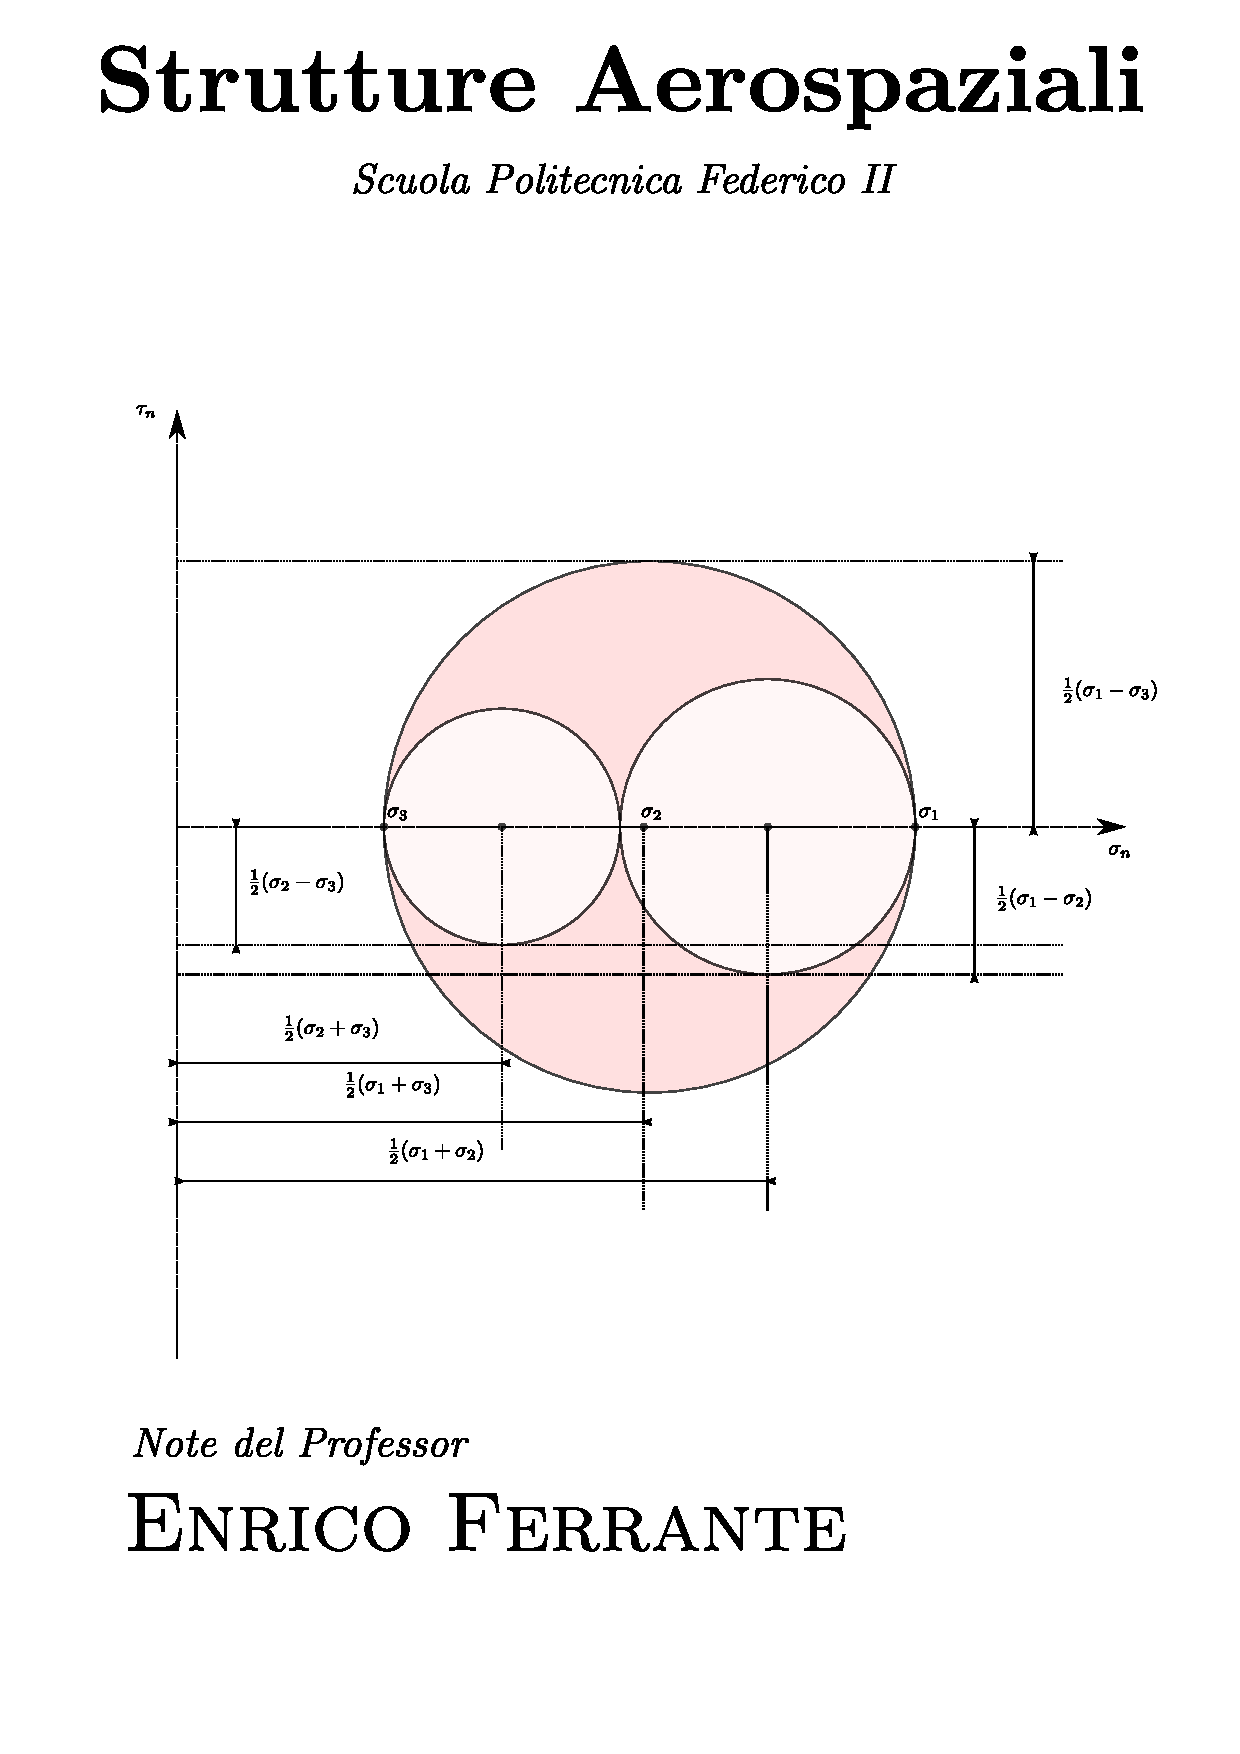
\includepdf[pages=-,pagecommand={},offset=10 -30]{Immagini/Frontespizio/Copertina_Ferrante.pdf}
\blankpage
%------------------------------------------------
%       FINE FRONTESPIZIO
%------------------------------------------------
%------------------------------------------------
%       INDICAZIONI PER LO SVILUPPO
%------------------------------------------------
\thispagestyle{plain}
\pagenumbering{gobble}
%%----------------------------------------------------------------------------------------
\pagestyle{plain}
%%----------------------------------------------------------------------------------------
%%       PREFAZIONE
%%----------------------------------------------------------------------------------------
\part*{Prefazione}
I \emph{pezzi} di cui un aereo è fatto sono collegati fra loro mediante chiodature, bullonature, incollaggi, saldature; quando l'aereo è in volo (e soprattutto in fase di manovra) forze di vario genere sollecitano \emph{pezzi} e \emph{collegamenti}: se questi sono stati costruiti senza un'adeguata metodologia, si può verificare una delle seguenti circostanze, sulla cui deprecabilità non vi è alcun dubbio: 
%----------------------------------------------------------------------------------------
\begin{itemize}
\item \emph{pezzi} e \emph{collegamenti} sono molto resistenti, ma molto \emph{grossi} (sovradimensionati) e l'aereo pesa troppo;
\item \emph{pezzi} e \emph{collegamenti} sono molto esili e leggeri ma si romperanno (o si deformeranno tanto da compremettere il funzionamento dell'aereo).
\end{itemize}
%----------------------------------------------------------------------------------------
Lo strutturista è chiamato a garantire che non si verifichi nessuna delle circostanze appena elencate; ciò si traduce nel fatto che egli deve essere in grado di gestire i seguenti due problemi:
%----------------------------------------------------------------------------------------
\begin{description}
\item[Verifica:] dato un elemento strutturale (\emph{pezzo} o \emph{collegamento}) di materiale e geometria noti, soggetto a carichi noti, determinare gli effetti che i carichi provocano in esso e, alla luce di questi ultimi, controllare che l'elemento (il \emph{pezzo}) resista con adeguati margini di sicurezza;
\item[Dimensionamento:] nota la forma di un elemento strutturale, prefissati alcuni parametri geometrici (quelli imposti dal suo \emph{ruolo}), scelto il materiale e noti i carichi che lo solleciteranno, individuare quali valori devono avere le sue dimensioni ancora \emph{in bianco} (cioè, che devono ancora essere determinate) affinché esso possa esercitare le proprie funzioni col minimo peso e adeguati margini di sicurezza.
\end{description}
%----------------------------------------------------------------------------------------
%\footnotesize{
%\paragraph{INDICAZIONI PER LO SVILUPPO DELLE ESERCITAZIONI A CASA\@.}~
%\\
%Il rispetto di queste indicazioni è tassativo. In presenza di difformità non prenderò in considerazione le relazioni. Ogni cosa riportata va letta con molta attenzione prima di essere sottoposta alla mia attenzione: non conviene ''usare'' un docente come correttore di bozze. 
%%----------------------------------------------------------------------------------------
%\paragraph{STESURA DEL TESTO (CON O SENZA WORD PROCESSOR)\@.} È richiesta un'esposizione strutturata piuttosto che narrativa. Pertanto descrivere sinteticamente ed in sequenza 
%%----------------------------------------------------------------------------------------
%\begin{itemize}
%\item lo scopo
%\item lo sviluppo
%\item l'applicazione
%\item le conclusioni
%\end{itemize}
%%----------------------------------------------------------------------------------------
%indicando gli strumenti (tecnici, informatici o scientifici) utilizzati per lo sviluppo e la stesura. È vietato riprodurre, anche in parte, la teoria alla base dell'esercizio: limitarsi all'indicazione bibliografica. La lunghezza, in facciate, del corpo del resoconto del lavoro a casa (escludendo quindi titolo, indice e lista dei simboli) va contenuta al massimo. 
%%----------------------------------------------------------------------------------------
%\paragraph{INDICAZIONI PARTICOLARI\@.} Il fascicolo che contiene gli esercizi deve essere curato, preciso, elegante, e pertanto
%%----------------------------------------------------------------------------------------
%\begin{itemize}
%\item i risultati numerici vanno riportati con la giusta accuratezza: porre \textbf{ESTREMA} attenzione all'aspetto delle cifre significative
%\item ogni rappresentazione grafica deve essere pertinente
%\item riportare sempre il sommario dei risultati in quadri sinottici od in opportuni grafici
%\item \textbf{FIGURE/DIAGRAMMI}\@. Figure in bianco, nero e toni di grigio (immagini e foto riprese da sorgenti bibliografiche, compresa la rete, potranno essere a colori). Inserire nel testo oppure alla fine, numerando e spaziando per bene, nel rispetto e con indicazione delle scale, con una legenda esauriente (= con tutte le indicazioni), senza sovrapporre la legenda ai grafici, usare simboli adeguatamente grandi. Il formato deve essere umano e l'assetto verticale. Ogni risultato in figura va commentato (nel testo od anche in didascalia). Il $C_d/C_D$ va misurato in \emph{Drag Count} e parte sempre da zero (lo stesso vale per la resistenza), ingrandire le polari nelle regioni di bassa resistenza
%\item Il disegno del profilo: \textbf{LE SCALE} (!), produrre una figura della larghezza utile della pagina, il tratto deve essere “corretto”
%\item evitare per quanto possibile termini in lingua diversa dall'italiano (un termine irrinunciabile di altra lingua va scritto in corsivo), evitare \emph{tout court} versioni italianizzate di termini di altre lingue
%\item nella stesura informatica lasciare un spazio bianco dopo i caratteri .\@,\@;\@?\@!\@; in stampa lasciare 3.5 cm a sinistra, 2 cm a destra
%\item eventuali formule vanno numerate
%\item non è necessario (ma può essere utile) riportare la lista dei simboli
%\item impiegare sempre una terminologia appropriata
%\item stare attenti ad evitare il costrutto “: (due punti) seguito da una figura o da una tabella”
%\item \textbf{CFD}\@. Le scale in toni di grigio. Congruità dei confronti con Xfoil: parità di $C_l$, rispetto dei limiti di validità 
%\item Scrivere sempre “numero di” Mach/Reynolds e non “Mach/Reynolds”.
%\end{itemize}
%%----------------------------------------------------------------------------------------
%\paragraph{PRESENTAZIONE\@.} Esercizi ed elaborati vanno presentati in un fascicolo non rilegato, indicando in copertina cognome, nome e matricola, insieme all’elenco di tutti gli esercizi in sviluppo o già convalidati, e riportando in seconda pagina le \textbf{INDICAZIONI PER LO SVILUPPO DELLE ESERCITAZIONI A CASA}\@. La forma è da me valutata in modo paritetico rispetto ai contenuti (e dunque leggere ogni cosa con molta attenzione prima di sottopormela). 
%%----------------------------------------------------------------------------------------
%\paragraph{CONTROLLO e CORREZIONE\@.} Io controllo e correggo solo testi~--~parziali o completi~--~purché già scritti in una forma definitiva (i.e.\ , non in bozza). Ovviamente il proponente procederà ad una preliminare autoverifica anche (e sopratutto) per gli aspetti formali\dots \\
%Interromperò il controllo di un esercizio alla prima violazione di una delle regole sopra riportate. È possibile sottopormi via mail il testo da controllare (in formato .pdf, dimensione $<500\,\,kb$).
%%----------------------------------------------------------------------------------------
%}
%%----------------------------------------------------------------------------------------

%------------------------------------------------
%       INDICAZIONI PER LO SVILUPPO
%------------------------------------------------
\clearpage
\tableofcontents
\clearpage
%------------------------------------------------
\pagenumbering{arabic}
\setcounter{page}{1}
%------------------------------------------------
%%----------------------------------------------------------------------------------------
\pagestyle{fancy}
%%----------------------------------------------------------------------------------------
%%       PREFAZIONE
%%----------------------------------------------------------------------------------------
\part{Momento statico, baricentro di figure piane}
\section{Introduzione}
\label{paragrafo1-1}
%----------------------------------------------------------------------------------------
\renewcommand{\thefigure}{1~-~1}
\begin{figure}[h]
\centering
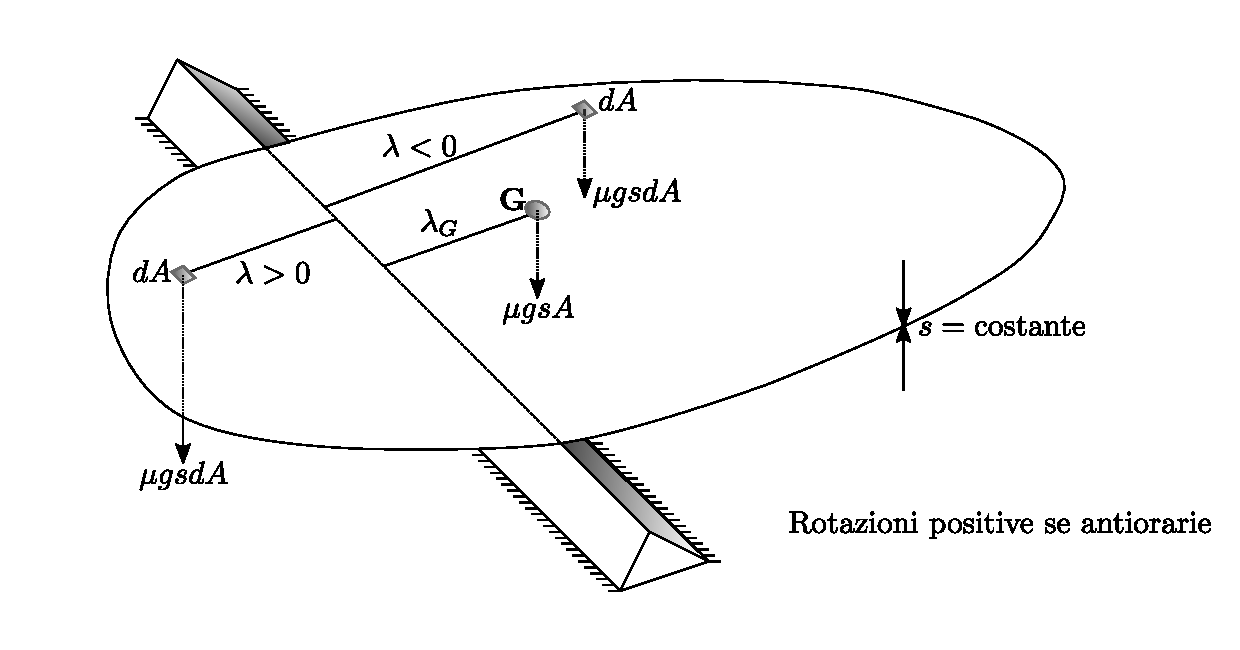
\includegraphics[width=\textwidth]{Immagini/Parte_1/Figura1_1/Figura1_1.pdf}
\caption{}
\label{figura1-1}
\end{figure}
%----------------------------------------------------------------------------------------
\noindent In figura~\ref{figura1-1} è rappresentato un \emph{lamierino} di materiale omogeneo, perfettamente piano, di spessore costante $s$; diciamo $A$ la sua area \emph{in pianta}. Esso è appoggiato su di una linea $r$ perfettamente orizzontale.
%----------------------------------------------------------------------------------------

\noindent La domanda sorge spontanea: il lamierino resterà in equilibrio oppure si ribalterà?
%----------------------------------------------------------------------------------------

\noindent Nel caso della figura la risposta è immediata: esso si ribalterà ruotando intorno alla retta $r$ in senso negativo (in figura si è assunto come verso positivo della rotazione intorno all'asse $r$ quello antiorario).
%----------------------------------------------------------------------------------------

\noindent Vogliamo approfondire, dal punto di vista fisico e matematico il tema in esame. Ogni \emph{pezzettino} di volume $d\mathcal{V}=sdA$ del lamierino ha una massa pari a 
%----------------------------------------------------------------------------------------
\begin{equation*}
dm = \mu sdA
\end{equation*}
%----------------------------------------------------------------------------------------
essendo $\mu$ la \textbf{densità} del materiale.
%----------------------------------------------------------------------------------------

\noindent In presenza di un campo gravitazionale (terrestre o no) su ogni \emph{pezzettino} agirà una forza gravitazionale diretta verso il basso pari 
%----------------------------------------------------------------------------------------
\begin{equation*}
\mu gsdA,
\end{equation*}
%----------------------------------------------------------------------------------------
essendo $g$ l'accelerazione di gravità (che sulla Terra vale $9.81\,\textup{m}/\textup{s}^2$). Ognuna delle suddette forze elementari ha un braccio $\lambda$ rispetto alla retta $r$ e, conseguentemente, ha un momento rispetto ad $r$ pari a 
%----------------------------------------------------------------------------------------
\begin{equation*}
\lambda \mu gsdA.
\end{equation*}
%----------------------------------------------------------------------------------------
\noindent Le forze che stanno a sinistra di $r$ hanno chiaramente un momento positivo (giacché esso promuove una rotazione positiva); ovviamente le forze che stanno a destra di $r$ hanno momento negativo. Si conviene pertanto di attribuire segno positivo alle distanze $\lambda$ delle areole a sinistra di $r$ (e di conseguenza segno negativo a quelle a destra di $r$). 
%----------------------------------------------------------------------------------------

\noindent Il momento risultante rispetto ad $r$ di tutte le forze elementari suddette vale pertanto 
%----------------------------------------------------------------------------------------
\begin{equation*}
M_r = \int\int_A \lambda \mu gsdA
\end{equation*}
%----------------------------------------------------------------------------------------

ed essendo $g$, $\mu$ ed $s$ costanti
%----------------------------------------------------------------------------------------
\begin{equation*}
M_r = \mu gs \int\int_A \lambda dA
\end{equation*}
%----------------------------------------------------------------------------------------

\noindent Naturalmente
%--------------------------------------------------------------------------------------------------------------------------------------------------
\begin{figure}[h!] 
\centering
\begin{tikzpicture}[scale=1.2, node distance=4cm,auto]
\node[block](init){Lamierino in equilibrio su $r$}; 
\node[](equal) at (1.70,0) {$=$};
\node[block, right of=init](var){$M_r=0$};
\node[](plus) at (5,0) {$=$};
\node[block, right of=var](var1){$\int\int_A \lambda dA=0$};
\end{tikzpicture}
\label{}
\end{figure}
%--------------------------------------------------------------------------------------------------------------------------------------------------

\noindent Come è noto, la risultante delle forze elementari $\mu gsdA$ è applicata nel \textbf{baricentro} (detto anche \textbf{centro di massa}) $\mathbf{G}$. 
%--------------------------------------------------------------------------------------------------------------------------------------------------

\noindent Detto $\lambda_G$ la distanza (con segno) di $\mathbf{G}$ da $r$, per il \textsc{Teorema di Varignon} risulta:
%--------------------------------------------------------------------------------------------------------------------------------------------------
\begin{figure}[h!] 
\centering
\begin{tikzpicture}[scale=1.2, node distance=4cm,auto]
\node[block](init){Mom. risultante rispetto ad $r$}; 
\node[](equal) at (1.70,0) {$=$};
\node[block, right of=init](var){Mom. della risultante rispetto ad $r$};
\end{tikzpicture}
\label{}
\end{figure}
%--------------------------------------------------------------------------------------------------------------------------------------------------

\noindent e pertanto 
%----------------------------------------------------------------------------------------
\begin{equation*}
M_r = \mu gs \lambda_G
\end{equation*}
%----------------------------------------------------------------------------------------

\noindent ovvero, semplificando 
%----------------------------------------------------------------------------------------
\begin{equation*}
\int\int_A \lambda dA = A \lambda_G
\end{equation*}
%----------------------------------------------------------------------------------------

\noindent e dunque 
%--------------------------------------------------------------------------------------------------------------------------------------------------
\begin{figure}[h!] 
\centering
\begin{tikzpicture}[scale=1.2, node distance=4cm,auto]
\node[block](init){Lamierino in equilibrio su $r$}; 
\node[](equal) at (1.70,0) {$=$};
\node[block, right of=init](var){$\lambda_G=0$};
\node[](plus) at (5,0) {$=$};
\node[block, right of=var](var1){$\mathbf{G}\in r$};
\end{tikzpicture}
\label{}
\end{figure}
%--------------------------------------------------------------------------------------------------------------------------------------------------
\section{La definizione di momento statico}
%----------------------------------------------------------------------------------------
\renewcommand{\thefigure}{1~-~2}
\begin{figure}[ht]
\centering
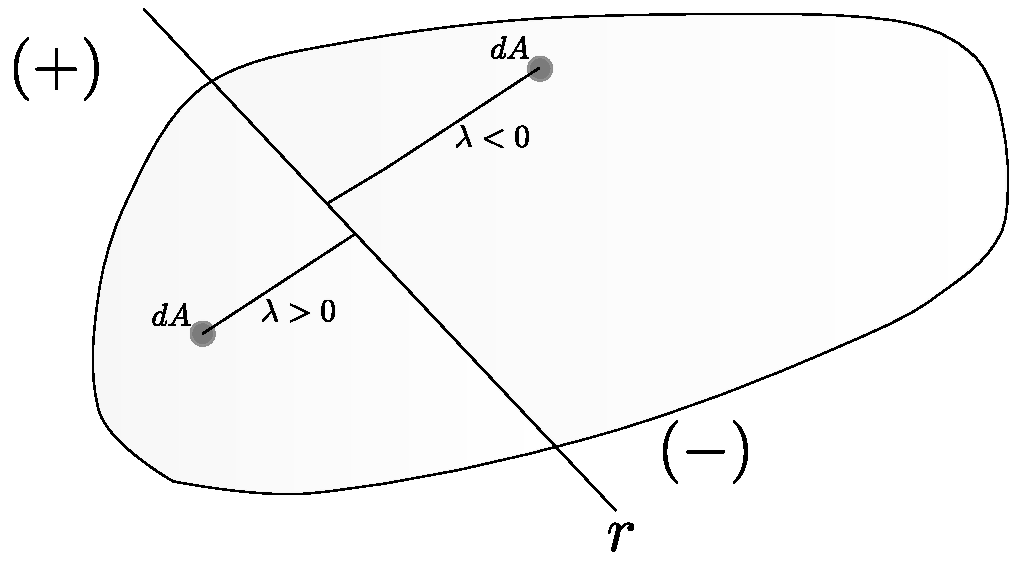
\includegraphics[width=0.55\textwidth]{Immagini/Parte_1/Figura1_2/Figura1_2.pdf}
\caption{}
\label{figura1-2}
\end{figure}
%----------------------------------------------------------------------------------------
\noindent In figura~\ref{figura1-2} è rappresentata una figura piana ed una retta $r$ ad essa complanare. Sia $dA$ una generica areola e $\lambda$ la sua distanza da $r$. Si sono assunte positive le distanze delle areole alla sinistra di $r$ (la scelta è arbitraria). Il prodotto $\lambda dA$ si dice \textbf{momento statico elementare} dell'areola $dA$ rispetto ad $r$. La quantità 
%---------------------------------------------------------------------------------------------------------------------------------------------
\begin{equation} \label{equazione1-1}
\boxed{S_r=\int\int_A \lambda dA}
\tag{1.1}
\end{equation}
%---------------------------------------------------------------------------------------------------------------------------------------------

\noindent si dice \textbf{Momento Statico} della figura rispetto ad $r$. 
%---------------------------------------------------------------------------------------------------------------------------------------------
%----------------------------------------------------------------------------------------
\renewcommand{\thefigure}{1~-~3}
\begin{figure}[h]
\centering
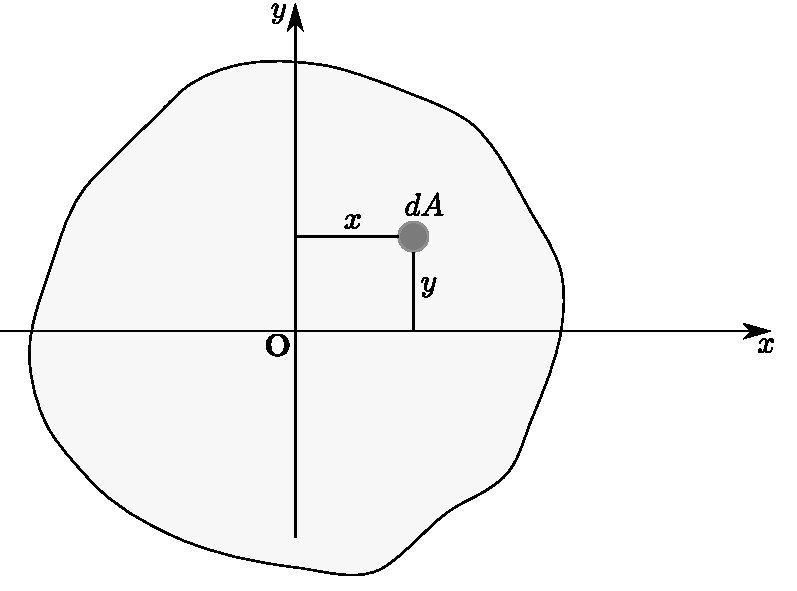
\includegraphics[width=0.5\textwidth]{Immagini/Parte_1/Figura1_3/Figura1_3.pdf}
\caption{}
\label{figura1-3}
\end{figure}
%----------------------------------------------------------------------------------------
\noindent Poiché l'integrale è, in effetti, la somma di tutti i termini elementari $\lambda dA$ presenti nel dominio piano invaso dalla figura, ed essi sono alcuni positivi ed alcuni negativi, si evince dalla~\eqref{equazione1-1} che può essere 
%---------------------------------------------------------------------------------------------------------------------------------------------
\begin{equation*}
\boxed{S_r\, \textup{maggiore, minore o uguale a zero}}
\end{equation*}
%---------------------------------------------------------------------------------------------------------------------------------------------

\noindent Nel caso specifico $S_r < 0$.
%---------------------------------------------------------------------------------------------------------------------------------------------

\noindent Sempre dalla~\eqref{equazione1-1} si evince che il momento statico ha dimensioni
%---------------------------------------------------------------------------------------------------------------------------------------------
\begin{equation*} 
[S_r]=[L]^3
\end{equation*}
%---------------------------------------------------------------------------------------------------------------------------------------------

\noindent e si misura pertanto in $\textup{m}^3$ (o $\textup{cm}^3$ o $\textup{mm}^3$). Il significato fisico di momento statico appare evidente alla luce di quanto detto nel precedente paragrafo: è immediato identificare una figura piana con un lamierino avente $\mu gs = 1$. Nel caso della figura~\ref{figura1-3} la~\eqref{equazione1-1} si particolarizza nelle: 
%---------------------------------------------------------------------------------------------------------------------------------------------
\begin{align} 
\label{equazione1-2}
S_x    &= \int\int_A ydA \tag{1.2a} \\
S_y    &= \int\int_A xdA \tag{1.2b}
\end{align}
%---------------------------------------------------------------------------------------------------------------------------------------------
\section{Baricentro di una figura piana}
%----------------------------------------------------------------------------------------
Per ogni figura piana esiste un punto (ed uno soltanto) che gode della seguente proprietà:
%----------------------------------------------------------------------------------------
%---------------------------------------------------------------------------------------------------------------------------------------------
\begin{equation*} 
\boxed{\textup{Rispetto ad ogni retta passante per esso è nullo il momento statico}}
\end{equation*}
%---------------------------------------------------------------------------------------------------------------------------------------------
Tale punto si dice \textbf{Baricentro} e sarà indicato con $\mathbf{G}$. 
%----------------------------------------------------------------------------------------
È immediato identificare il baricentro di una figura piana con il centro di massa di un lamierino avente la stessa forma in pianta (purché di spessore costante e materiale omogeneo). E allora, in forza di quanto detto al paragrafo~\vref{paragrafo1-1}, possiamo affermare che 
%---------------------------------------------------------------------------------------------------------------------------------------------
\begin{equation} 
\label{equazione1-3}
\boxed{S_r = A\lambda_G}
\tag{1.3}
\end{equation}
%---------------------------------------------------------------------------------------------------------------------------------------------
%----------------------------------------------------------------------------------------
\renewcommand{\thefigure}{1~-~4}
\begin{figure}[h]
\centering
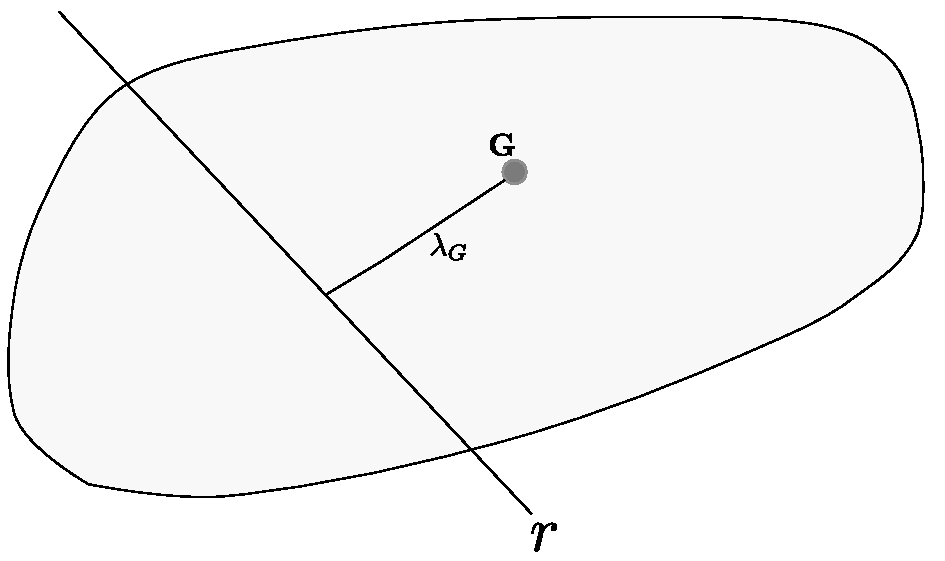
\includegraphics[width=0.5\textwidth]{Immagini/Parte_1/Figura1_4/Figura1_4.pdf}
\caption{}
\label{figura1-4}
\end{figure}
%----------------------------------------------------------------------------------------
La figura~\ref{figura1-4} chiarisce definitivamente quanto appena detto. La~\eqref{equazione1-3} è di notevole importanza: essa consente di calcolare il momento statico $S_r$ senza fare integrali, a patto di conoscere la posizione del baricentro $\mathbf{G}$. 
%----------------------------------------------------------------------------------------

\noindent A questo punto è ovvio che valgono le relazioni 
%---------------------------------------------------------------------------------------------------------------------------------------------
\begin{align} 
S_x    &= Ay_G \tag{1.4a} \label{equazione1-4a} \\
S_y    &= Ax_G \tag{1.4b} \label{equazione1-4b}
\end{align}
%---------------------------------------------------------------------------------------------------------------------------------------------
\renewcommand{\thefigure}{1~-~5}
\begin{figure}[h]
\centering
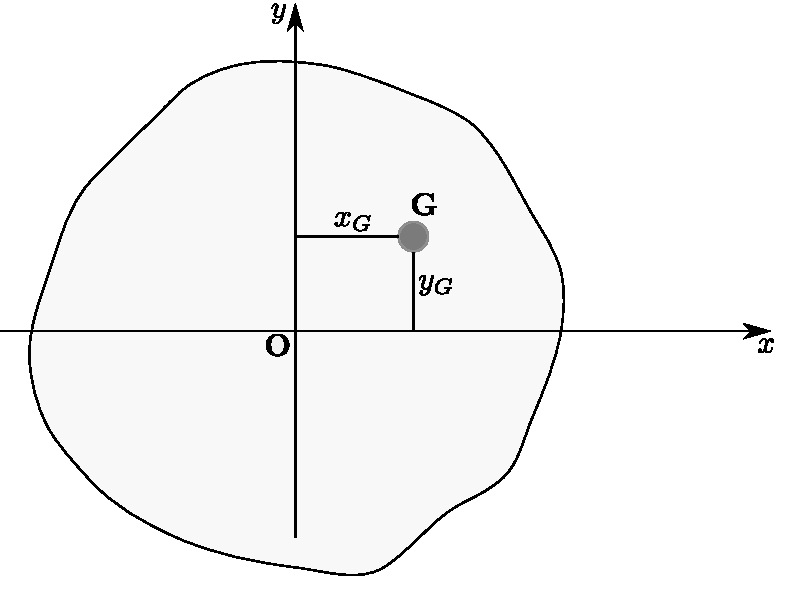
\includegraphics[width=0.5\textwidth]{Immagini/Parte_1/Figura1_5/Figura1_5.pdf}
\caption{}
\label{figura1-5}
\end{figure}
%----------------------------------------------------------------------------------------
%----------------------------------------------------------------------------------------

\noindent Ancora una volta, la figura~\ref{figura1-5} chiarisce quanto appena detto. A proposito di baricentro, si potrebbe dimostrare la seguente proposizione, peraltro intuitiva:
%---------------------------------------------------------------------------------------------------------------------------------------------
\begin{equation*} 
\boxed{\textup{Se una figura possiede due o più assi di simmetria (ortogonali o no)}\,\mathbf{G}\,\textup{è nella loro intersezione}}
\end{equation*}
%---------------------------------------------------------------------------------------------------------------------------------------------
%---------------------------------------------------------------------------------------------------------------------------------------------
\renewcommand{\thefigure}{1~-~6}
\begin{figure}[h]
\centering
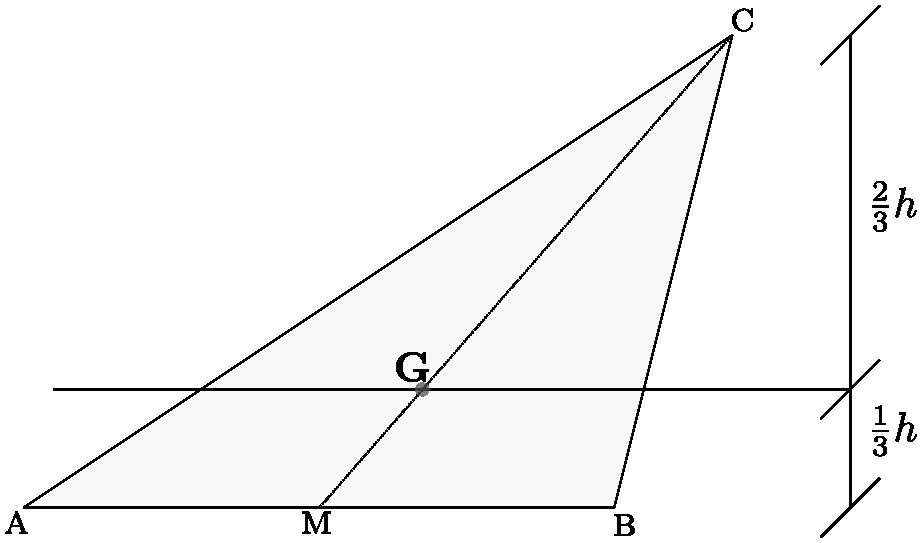
\includegraphics[width=0.5\textwidth]{Immagini/Parte_1/Figura1_6/Figura1_6.pdf}
\caption{}
\label{figura1-6}
\end{figure}
%----------------------------------------------------------------------------------------

\noindent Quest'ultima proposizione consente di individuare il baricentro di numerose figure, tra cui il triangolo (anche scaleno). 

\noindent Con riferimento alla figura~\ref{figura1-6}, la mediana \textsc{cm} è asse di simmetria rispetto alla direzione del lato \textsc{ab}: essa, infatti, dimezza tutti i segmenti interni al triangolo e paralleli al lato \textsc{ab}. 

\noindent Pertanto, in forza della precedente proposizione, il baricentro di un triangolo qualunqe è nelle intersezioni delle tre mediane. E ciò, con semplici considerazione geometriche, porta a concludere che la distanza di $\mathbf{G}$ da ogni lato del triangolo è uguale ad $1/3$ dell'altezza relativa al lato in questione. 
%---------------------------------------------------------------------------------------------------------------------------------------------
\renewcommand{\thefigure}{1~-~7}
\begin{figure}[h]
\centering
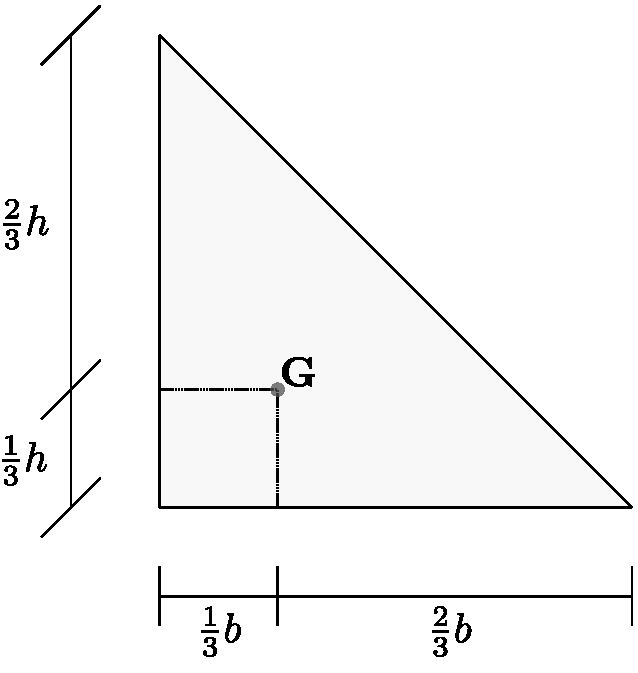
\includegraphics[width=0.45\textwidth]{Immagini/Parte_1/Figura1_7/Figura1_7.pdf}
\caption{}
\label{figura1-7}
\end{figure}
%----------------------------------------------------------------------------------------
\noindent La figura~\ref{figura1-7} illustra il caso del triangolo rettangolo.

\noindent Per determinare il baricentro di una figura piana qualunque si procede così:
%----------------------------------------------------------------------------------------
\begin{enumerate}
\item si assumono due assi di riferimento $x$ ed $y$ scelti a piacere
\item si suddivide la figura in figure parziali (di ognuna delle quali si conosca il baricentro e si sappia calcolare l'area $A_i$)
\item si calcolano $S_{ix}$ ed $S_{iy}$ (momenti statici della generica figura parziale)
\item si calcolano:
\begin{align*}
A    &= \sum_{i=1}^n A_i \\
S_x &= \sum_{i=1}^n S_{ix} \\
S_y &= \sum_{i=1}^n S_{iy}
\end{align*}
\item dalle~\eqref{equazione1-4a} e~\eqref{equazione1-4b} si ricava immediatamente 
%---------------------------------------------------------------------------------------------------------------------------------------------
\begin{align} 
x_G    &= \frac{S_y}{A} \tag{1.5a} \label{equazione1-5a} \\
y_G    &= \frac{S_x}{A} \tag{1.5b} \label{equazione1-5b}
\end{align}
%---------------------------------------------------------------------------------------------------------------------------------------------
\end{enumerate}
%----------------------------------------------------------------------------------------

\noindent Le uguaglianze scritte al punto $4.$ della procedura appena illustrata, sono legittimate dalla ben nota proprietà di additività degli integrali definiti (e tali sono $A$, $S_x$ ed $S_y$).
%----------------------------------------------------------------------------------------
\clearpage
\section{Esercizi}
%----------------------------------------------------------------------------------------
\paragraph{Esercizio 1.1}
%----------------------------------------------------------------------------------------
Determinare il baricentro del profilato illustrato in figura.
%---------------------------------------------------------------------------------------------------------------------------------------------
\renewcommand{\thefigure}{1.1~-~1}
\begin{figure}[h]
\centering
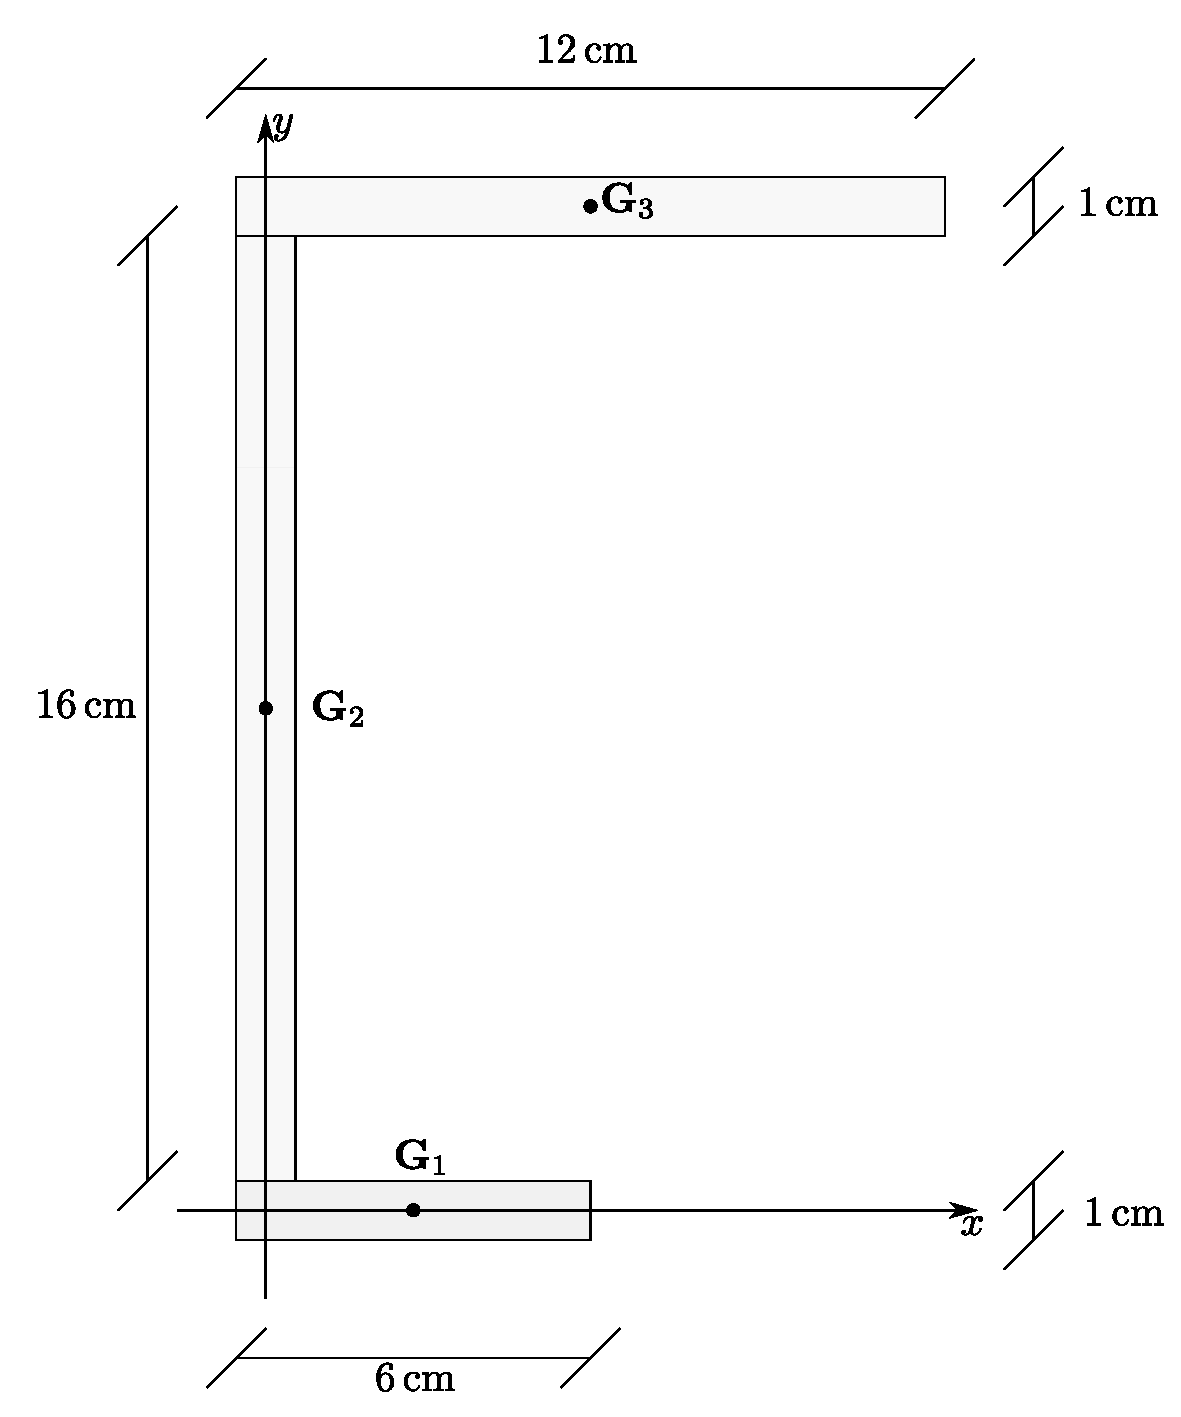
\includegraphics[width=0.80\textwidth]{Immagini/Parte_1/Esercizio1_1/Esercizio1_1.pdf}
\caption{}
\label{Esercizio1_1_1}
\end{figure}
%----------------------------------------------------------------------------------------

\noindent Il profilato è ovviamente interpretabile come unione di $3$ rettangoli (i cui baricentri si sono indicati con $\mathbf{G}_1$, $\mathbf{G}_2$ e $\mathbf{G}_3$). 

\noindent I due assi di riferimento assunti sono certamente quelli che consentono la massima semplificazione nel calcolo dei momenti statici. Risulta dunque:
%----------------------------------------------------------------------------------------
\begin{equation*}
\begin{aligned}
A &= 6\,\textup{cm}^2 \\
A &= 16\,\textup{cm}^2 \\
A &= 12\,\textup{cm}^2
\end{aligned}
\,\,\Biggr\}\,\, A = 34\,\textup{cm}^2
\end{equation*}
%----------------------------------------------------------------------------------------
%----------------------------------------------------------------------------------------
\begin{equation*}
\begin{aligned}
S_{1x} &= 0\,\textup{cm}^3 \\
S_{2x} &= 16\times 8.5 = 136\,\textup{cm}^3 \\
S_{3x} &= 12\times 17  = 204\,\textup{cm}^3
\end{aligned}
\,\,\Biggr\}\,\, S_x = 340\,\textup{cm}^3
\end{equation*}
%----------------------------------------------------------------------------------------
%----------------------------------------------------------------------------------------
\begin{equation*}
\begin{aligned}
S_{1y} &= 6\times 2.5 = 15\,\textup{cm}^3 \\
S_{2y} &= 0\,\textup{cm}^3 \\
S_{3y} &= 12\times 5.5  = 66\,\textup{cm}^3
\end{aligned}
\,\,\Biggr\}\,\, S_y = 81\,\textup{cm}^3
\end{equation*}
%----------------------------------------------------------------------------------------
Pertanto, applicando le equazioni~\eqref{equazione1-5a} e~\eqref{equazione1-5b}:
%---------------------------------------------------------------------------------------------------------------------------------------------
\begin{align*} 
x_G    &= \frac{S_y}{A} = \frac{81}{34} = 2.38\,\textup{cm}  \\
y_G    &= \frac{S_x}{A} = \frac{340}{34} = 10\,\textup{cm}
\end{align*}
%---------------------------------------------------------------------------------------------------------------------------------------------
%---------------------------------------------------------------------------------------------------------------------------------------------
\renewcommand{\thefigure}{1.1~-~2}
\begin{figure}[h]
\centering
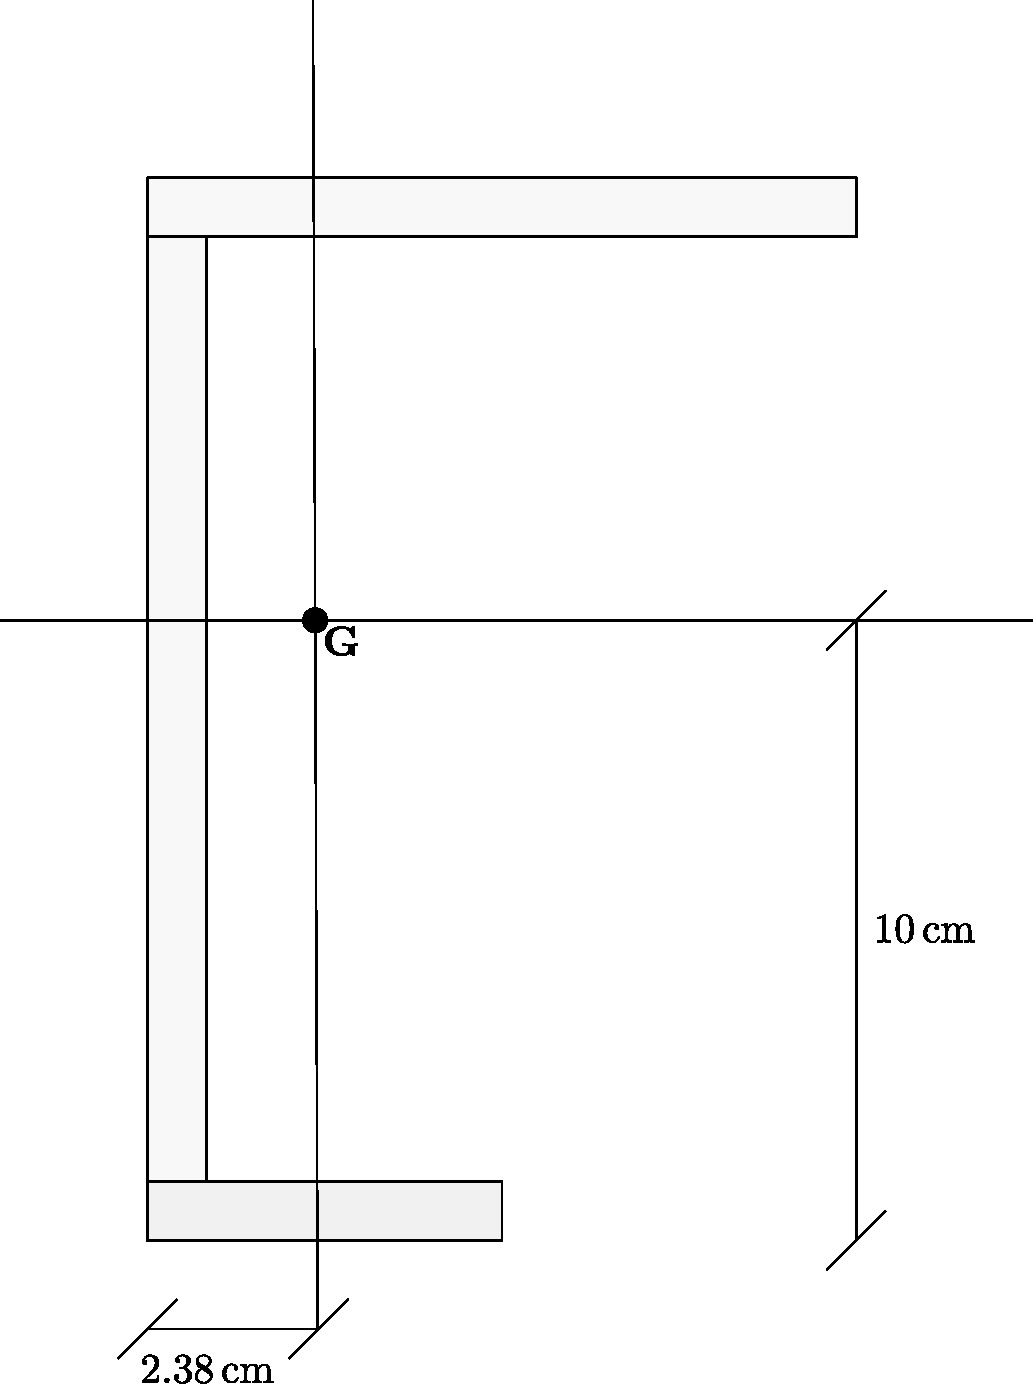
\includegraphics[width=0.45\textwidth]{Immagini/Parte_1/Esercizio1_1/Esercizio1_1_2.pdf}
\caption{}
\label{Esercizio1_1_2}
\end{figure}
%----------------------------------------------------------------------------------------
\paragraph{Esercizio 1.2}
Determinare il baricentro della figura assegnata avendo presente che il cerchio è un foro. 
%---------------------------------------------------------------------------------------------------------------------------------------------
\renewcommand{\thefigure}{1.2~-~1}
\begin{figure}[h]
\centering
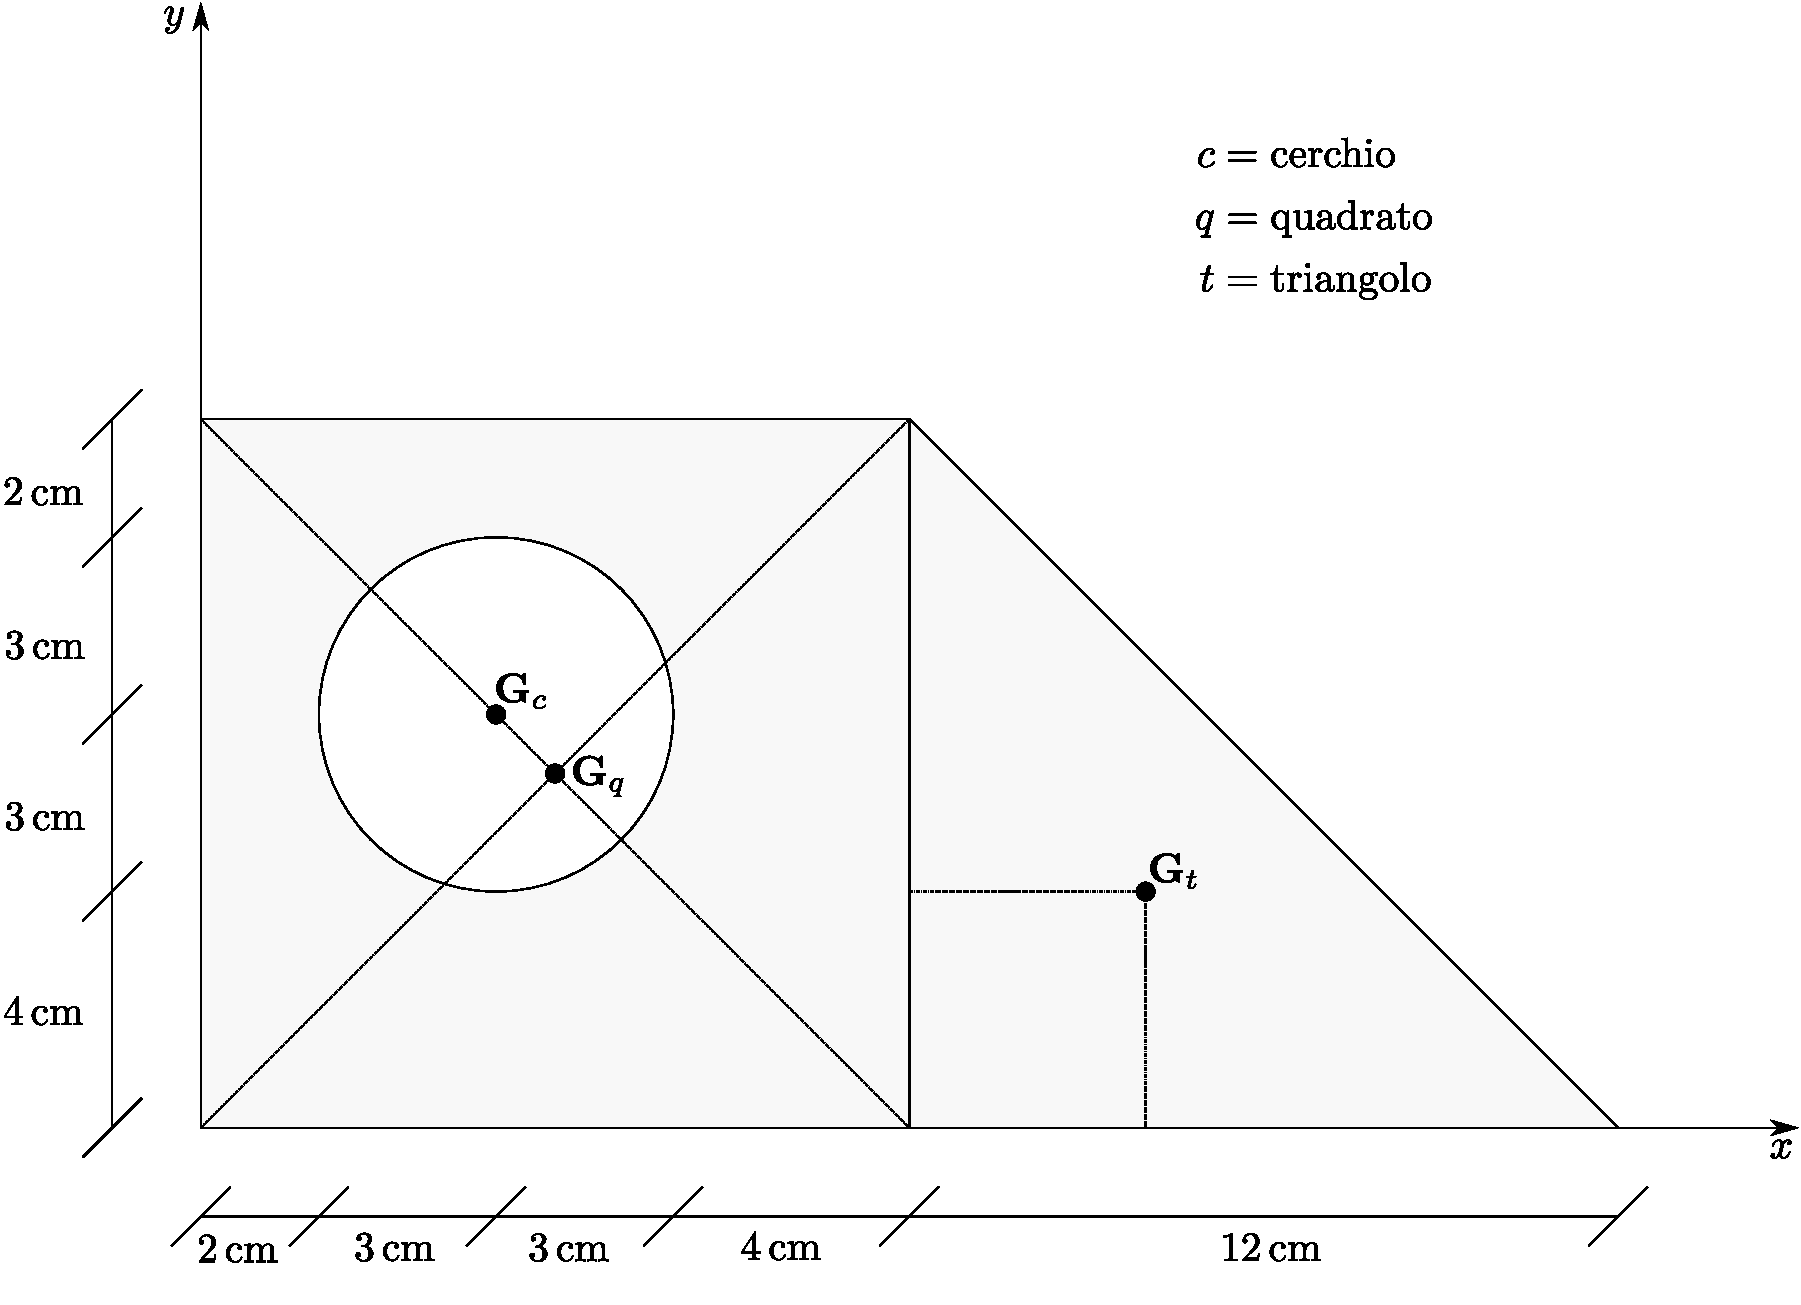
\includegraphics[width=0.89\textwidth]{Immagini/Parte_1/Esercizio1_2/Esercizio1_2_1.pdf}
\caption{}
\label{Esercizio1_2}
\end{figure}
%----------------------------------------------------------------------------------------
%----------------------------------------------------------------------------------------
\begin{equation*}
\begin{aligned}
A_t &= \frac{1}{2}12^2 = 72\,\textup{cm}^2 \\
A_q &= 12^2 = 144\,\textup{cm}^2 \\
A_c &= \pi3^2 = 28.26\,\textup{cm}^2
\end{aligned}
\,\,\Biggr\}\,\, A = 72+144-28.26 = 187.74\,\textup{cm}^2
\end{equation*}
%----------------------------------------------------------------------------------------
%----------------------------------------------------------------------------------------
\begin{equation*}
\begin{aligned}
S_{\textup{t}x} &= 72\times 4 = 288\,\textup{cm}^3 \\
S_{\textup{q}x} &= 144\times 6 = 864\,\textup{cm}^3 \\
S_{\textup{c}x} &= 28.26\times 17  = 480.42\,\textup{cm}^3
\end{aligned}
\,\,\Biggr\}\,\, S_x = 288+864-480.42 = 671.58\,\textup{cm}^3
\end{equation*}
%----------------------------------------------------------------------------------------
%----------------------------------------------------------------------------------------
\begin{equation*}
\begin{aligned}
S_{\textup{t}y} &= 72\times 16 = 1152\,\textup{cm}^3 \\
S_{\textup{q}y} &= 144\times 6 = 864\,\textup{cm}^3 \\
S_{\textup{c}y} &= 28.26\times 5  = 141.30\,\textup{cm}^3
\end{aligned}
\,\,\Biggr\}\,\, S_y = 1152+864-141.30 = 1874.70\,\textup{cm}^3
\end{equation*}
%----------------------------------------------------------------------------------------
%---------------------------------------------------------------------------------------------------------------------------------------------
\begin{align*} 
x_G    &= \frac{S_y}{A} = \frac{1874.70}{187.74} = 9.986\,\textup{cm}  \\
y_G    &= \frac{S_x}{A} = \frac{951.31}{187.74} = 5.067\,\textup{cm}
\end{align*}
%---------------------------------------------------------------------------------------------------------------------------------------------
\paragraph{Esercizio 1.3}
Formulare i momenti statici e la posizione del baricentro per il settore di corona circolare rappresentato in figura.
%---------------------------------------------------------------------------------------------------------------------------------------------
\renewcommand{\thefigure}{1.3~-~1}
\begin{figure}[ht]
\centering
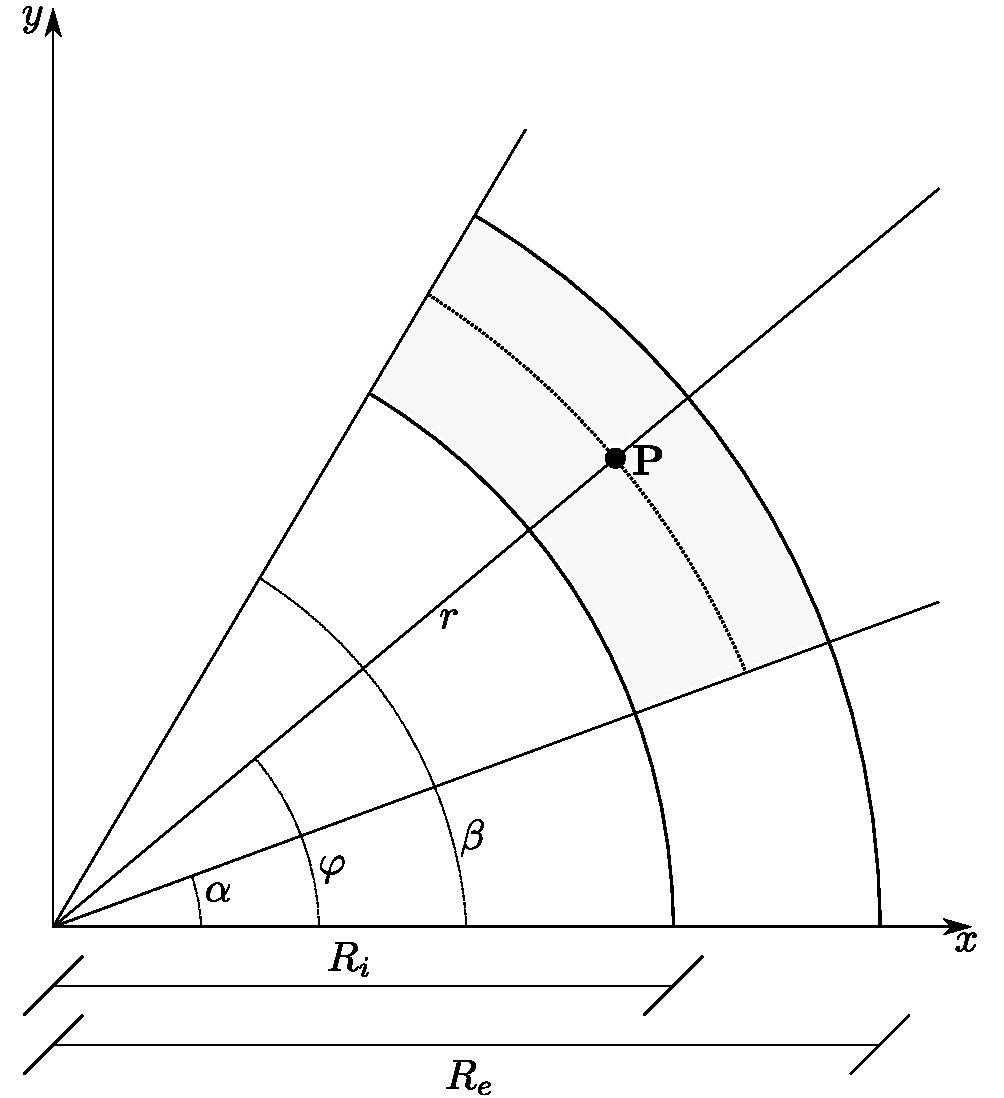
\includegraphics[width=0.8\textwidth]{Immagini/Parte_1/Esercizio1_3/Esercizio1_3.pdf}
\caption{}
\label{Esercizio1_3}
\end{figure}
%----------------------------------------------------------------------------------------

\noindent Sappiamo che 
%----------------------------------------------------------------------------------------
\begin{equation*}
A = \frac{\beta-\alpha}{2}(R_e^2-R_i^2)
\end{equation*}
%----------------------------------------------------------------------------------------
Per conoscere $S_x$ ed $S_y$ dobbiamo calcolare gli integrali: 
%----------------------------------------------------------------------------------------
\begin{align*}
S_x &= \int\int_A ydA \\
S_y &= \int\int_A xdA
\end{align*}
%----------------------------------------------------------------------------------------
Naturalmente conviene introdurre le coordinate polari: 
%----------------------------------------------------------------------------------------
\begin{equation*}
\,\,\Biggr\{\,\, 
\begin{aligned}
x &= r\cos\varphi \\
y &= r\sin\varphi
\end{aligned}
\end{equation*}
%----------------------------------------------------------------------------------------
Lo \emph{Jacobiano} della trasformazione $(x,\,y)\,\leftrightarrow\,(r,\,\varphi)$ vale: 
%----------------------------------------------------------------------------------------
\begin{equation*}
\lvert \, J \, \lvert =
\begin{vmatrix}
\frac{\partial x}{\partial r} & \frac{\partial y}{\partial r}\\
\frac{\partial x}{\partial\varphi} & \frac{\partial y}{\partial\varphi}
\end{vmatrix}
=
\begin{vmatrix}
\cos\varphi & \sin\varphi \\
-r\sin\varphi & r\cos\varphi
\end{vmatrix}
= r
\end{equation*}
%----------------------------------------------------------------------------------------
E dunque
%----------------------------------------------------------------------------------------
\begin{align*}
S_x &= \int\int_A ydxdy = \int\int_A r\sin\varphi rdrd\varphi = \int_{R_{i}}^{R_{e}} r^2dr\int_\alpha^\beta \sin\varphi d\varphi = \frac{1}{3}(R_e^3-R_i^3)(\cos\alpha-\cos\beta) \\
S_y &= \int\int_A xdxdy = \int\int_A r\cos\varphi rdrd\varphi = \int_{R_{i}}^{R_{e}} r^2dr\int_\alpha^\beta \cos\varphi d\varphi = \frac{1}{3}(R_e^3-R_i^3)(\sin\beta-\sin\alpha) 
\end{align*} 
%----------------------------------------------------------------------------------------
Le coordinate del baricentro sono, pertanto: 
%---------------------------------------------------------------------------------------------------------------------------------------------
\begin{align*} 
x_G    &= \frac{S_y}{A} = \frac{2}{3} \frac{(R_e^3-R_i^3)}{(R_e^2-R_i^2)}\frac{(\sin\beta-\sin\alpha)}{\beta-\alpha}  \\
y_G    &= \frac{S_x}{A} = \frac{2}{3} \frac{(R_e^3-R_i^3)}{(R_e^2-R_i^2)}\frac{(\cos\alpha-\cos\beta)}{\beta-\alpha}
\end{align*}
%---------------------------------------------------------------------------------------------------------------------------------------------
Vale la pena di sottolineare che il settore di corona circolare ha un asse di simmetria ortogonale; il baricentro, ovviamente, sta su tale asse e la sua distanza dal centro (che è l'origine del riferimento) è ovviamente:%---------------------------------------------------------------------------------------------------------------------------------------------
\begin{equation*}
d_G = \sqrt{x_G^2+y_G^2}
\end{equation*}
%---------------------------------------------------------------------------------------------------------------------------------------------
Utilizzando le precedenti formulazioni di $x_G$ ed $y_G$ con semplici passaggi si trova:
%---------------------------------------------------------------------------------------------------------------------------------------------
\begin{equation*}
d_G = \frac{2}{3}\frac{(R_e^3-R_i^3)}{(R_e^2-R_i^2)}\frac{\sin\frac{\beta-\alpha}{2}}{\frac{\beta-\alpha}{2}}
\end{equation*}
%---------------------------------------------------------------------------------------------------------------------------------------------
\clearpage
%---------------------------------------------------------------------------------------------------------------------------------------------
\paragraph{Esercizio 1.4}
Determinare il baricentro del quarto di cerchio rappresentato in figura e calcolarne $S_x$ ed $S_y$.
%---------------------------------------------------------------------------------------------------------------------------------------------
\renewcommand{\thefigure}{1.4~-~1}
\begin{figure}[ht]
\centering
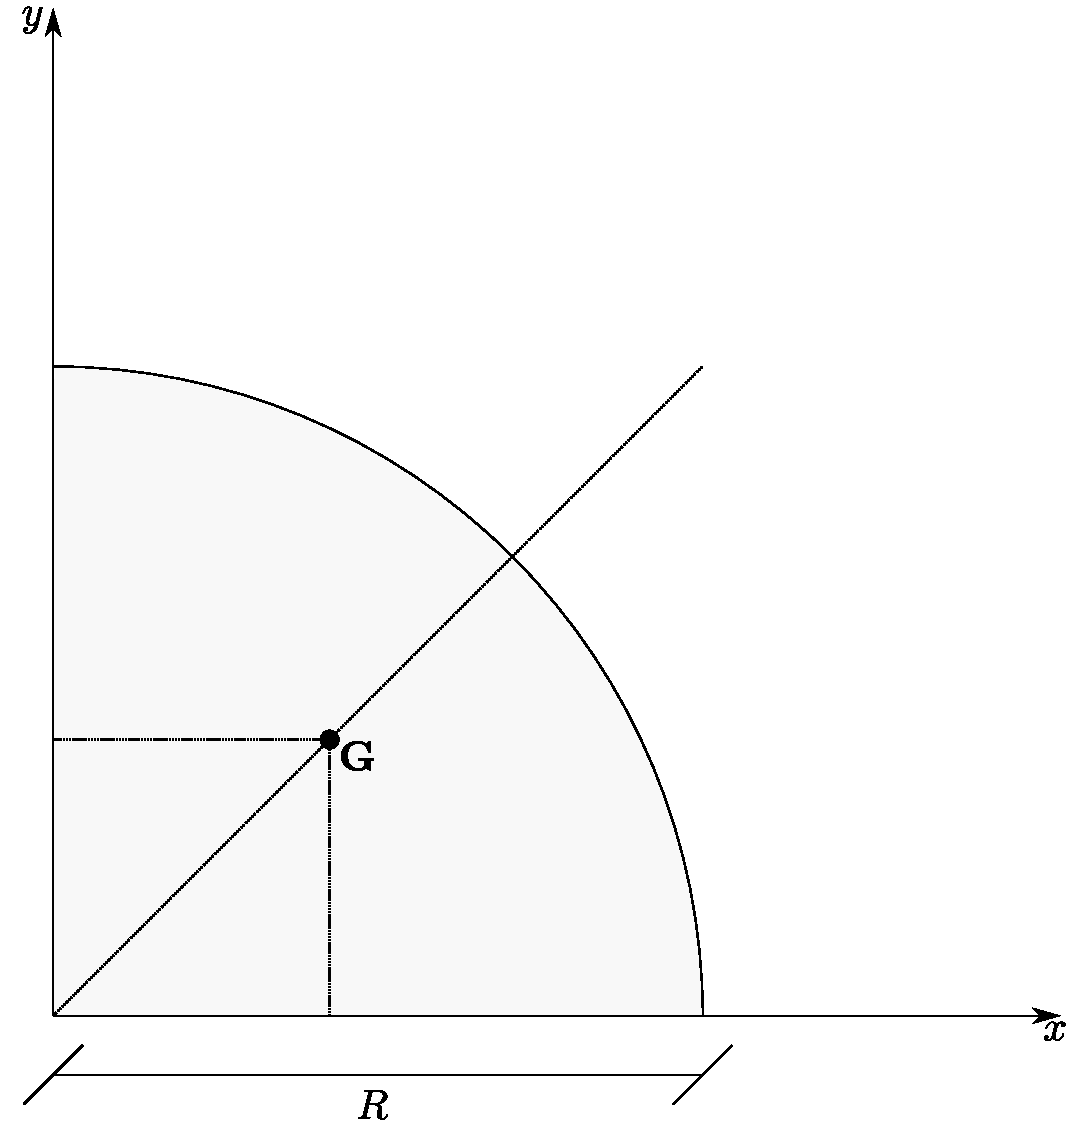
\includegraphics[width=0.6\textwidth]{Immagini/Parte_1/Esercizio1_4/Esercizio1_4.pdf}
\caption{}
\label{Esercizio1_4}
\end{figure}
%----------------------------------------------------------------------------------------
Per calcolare la distanza del baricentro dal centro possiamo applicare la formula per $d_G$ trovata nell'esercizio precedente, ponendo in essa: 
%----------------------------------------------------------------------------------------
\begin{align*}
R_e &= R \\ 
R_i &= 0 \\
\alpha &= 0 \\ 
\beta &=\frac{\pi}{2}
\end{align*}
%----------------------------------------------------------------------------------------
E così si trova: 
%----------------------------------------------------------------------------------------
\begin{equation*}
\lvert \, \textup{OG} \, \lvert = \frac{2}{3}R\frac{\sin\frac{\pi}{4}}{\frac{\pi}{4}} = \frac{4\sqrt{2}}{3\pi}R = 0.6R 
\end{equation*}
%----------------------------------------------------------------------------------------
Le coordinate del baricentro $\mathbf{G}$ sono, ovviamente: 
%----------------------------------------------------------------------------------------
\begin{equation*}
x_G = y_G = \frac{\sqrt{2}}{2}d_G = \frac{4}{3\pi}R = 0.4244R
\end{equation*}
%----------------------------------------------------------------------------------------
Naturalmente, risulta:
%----------------------------------------------------------------------------------------
\begin{equation*}
S_x = S_y = A\times x_G = \frac{\pi}{4}R^2\frac{4}{3\pi}R = \frac{1}{3}R^3
\end{equation*}
%----------------------------------------------------------------------------------------
\paragraph{Esercizio 1.5}
%----------------------------------------------------------------------------------------
Determinare il baricentro del semicerchio rappresentato in figura e calcolarne $S_x$ ed $S_y$. 
%----------------------------------------------------------------------------------------
%---------------------------------------------------------------------------------------------------------------------------------------------
\renewcommand{\thefigure}{1.5~-~1}
\begin{figure}[ht]
\centering
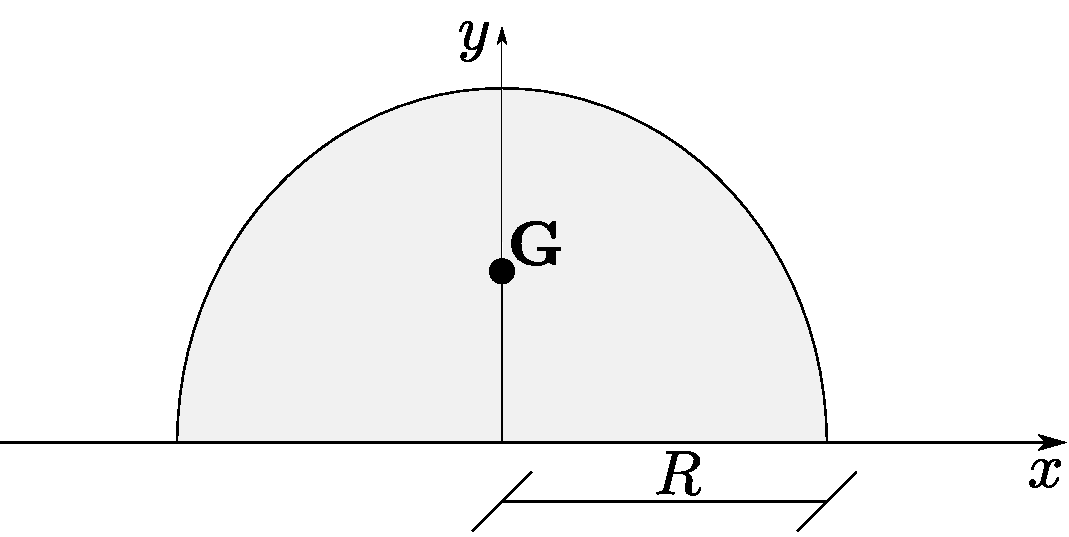
\includegraphics[width=\textwidth]{Immagini/Parte_1/Esercizio1_5/Esercizio1_5.pdf}
\caption{}
\label{Esercizio1_5}
\end{figure}
%----------------------------------------------------------------------------------------

\noindent Sarà ovviamente 
%----------------------------------------------------------------------------------------
\begin{align*}
x_G &= 0 \\ 
S_y &= 0
\end{align*}
%----------------------------------------------------------------------------------------
Per calcolare $y_G$ possiamo utilizzare la formula ricavata nell'Esercizio 1.3 ponendo in essa: 
%----------------------------------------------------------------------------------------
\begin{align*}
R_e &= R \\ 
R_i &= 0 \\
\alpha &=0 \\ 
\beta &=\pi
\end{align*}
%----------------------------------------------------------------------------------------
E così si trova:
%----------------------------------------------------------------------------------------
\begin{equation*}
y_G = \frac{2}{3}R\frac{\cos 0 - \cos\pi}{\pi-0} = \frac{4}{3\pi}R \approx 0.4244R
\end{equation*}
%----------------------------------------------------------------------------------------
Com'era lecito attendersi, $y_G$ è uguale a quella relativa ad un quarto di cerchio. Ovviamente: 
%----------------------------------------------------------------------------------------
\begin{equation*}
S_x = A\times y_G = \frac{\pi}{2}R^2\frac{4}{3\pi}R = \frac{2}{3}R
\end{equation*}
%----------------------------------------------------------------------------------------
\clearpage
\paragraph{Esercizio 1.6}
%----------------------------------------------------------------------------------------
Determinare il baricentro della zona ombreggiata rappresentata in figura. 
%---------------------------------------------------------------------------------------------------------------------------------------------
\renewcommand{\thefigure}{1.6~-~1}
\begin{figure}[h]
\centering
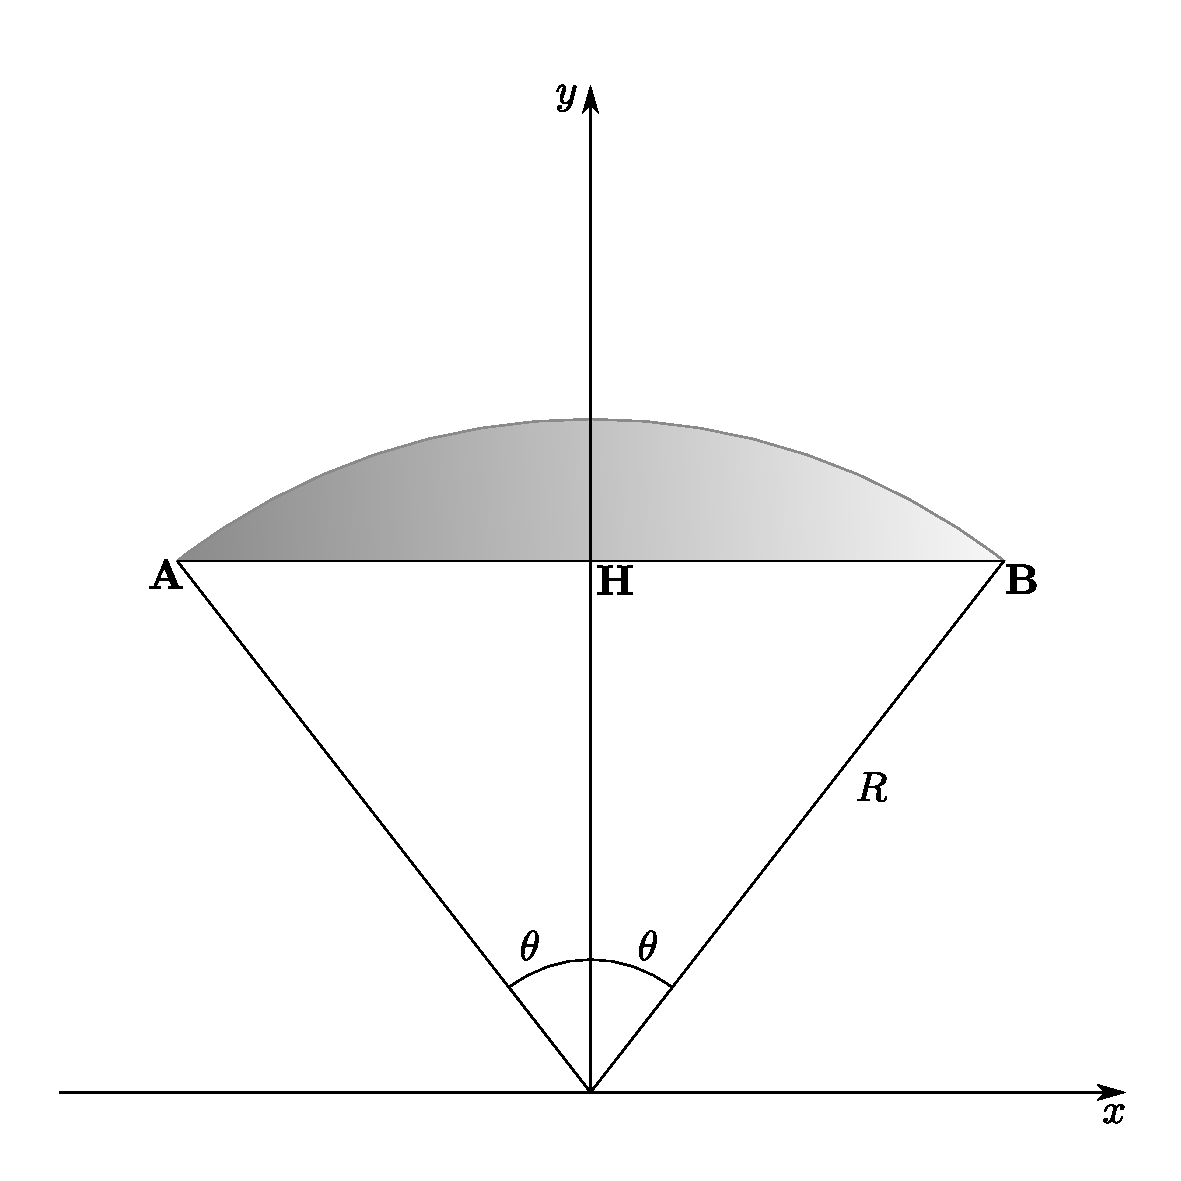
\includegraphics[width=0.75\textwidth]{Immagini/Parte_1/Esercizio1_6/Esercizio1_6.pdf}
\caption{}
\label{Esercizio1_6}
\end{figure}
%----------------------------------------------------------------------------------------

\noindent È evidente che $x_G=0$. Per calcolare $y_G$ ci servono $S_x$ ed $A$; sia $S_x$ che $A$ possono calcolarsi per differenza: 
%----------------------------------------------------------------------------------------
\begin{align*}
A &= \textup{Area settore ombreggiato} - \textup{Area triangolo} = A_s - A_t \\
S_x &= S_{\textup{s}x} - S_{\textup{t}x}
\end{align*}
%----------------------------------------------------------------------------------------
Dalla figura si ha: 
%----------------------------------------------------------------------------------------
\begin{align*}
A_s &= \theta R^2 \\ 
A_t &= \frac{1}{2}\, \lvert \, \textup{AB} \, \lvert \, \lvert \, \textup{OH} \, \lvert = R^2 \sin\theta\cos\theta
\end{align*}
%----------------------------------------------------------------------------------------
da cui 
%----------------------------------------------------------------------------------------
\begin{equation*}
A = (\theta-\sin\theta\cos\theta)R^2
\end{equation*}
%----------------------------------------------------------------------------------------
Per calcolare $S_{\textup{s}x}$ possiamo utilizzare la formula ricavata nell'esercizio 1.3 ponendo in essa:
%----------------------------------------------------------------------------------------
\begin{align*}
R_e &= R \\
R_i &= 0 \\
\alpha &= \frac{\pi}{2}-\theta \\ 
\beta &= \frac{\pi}{2}+\theta
\end{align*}
%----------------------------------------------------------------------------------------
E così si trova:
%----------------------------------------------------------------------------------------
\begin{align*}
S_{\textup{s}x} &= \frac{1}{3}\Biggr[\cos\biggl(\frac{\pi}{2}-\theta\biggr)-\cos\biggl(\frac{\pi}{2}+\theta\biggr)\Biggl]=\frac{2}{3}R^3 \sin\theta \\
S_{\textup{t}x} &= \frac{2}{3}A_t\, \lvert \, \textup{OH} \, \lvert =R^2 \sin\theta\cos\theta\frac{2}{3}R\cos\theta =\frac{2}{3}R^3 \sin\theta\cos^{2}\theta
\end{align*}
%----------------------------------------------------------------------------------------
Quindi:
%----------------------------------------------------------------------------------------
\begin{equation*}
S_x = S_{\textup{s}x}-S_{\textup{t}x} = \frac{2}{3}R^3 \sin\theta - \frac{2}{3}R^3 \sin\theta\cos^{2}\theta = \frac{2}{3}R^3 \sin^{3}\theta
\end{equation*}
%----------------------------------------------------------------------------------------
In definitiva:
%----------------------------------------------------------------------------------------
\begin{equation*}
y_G = \frac{S_x}{A} = \frac{2}{3}R^{3}\sin^{3}\theta\frac{1}{R^{2}(\theta-\sin\theta\cos\theta)}
\end{equation*}
%----------------------------------------------------------------------------------------
e semplificando
%----------------------------------------------------------------------------------------
\begin{equation*}
y_G = \frac{S_x}{A} = \frac{2}{3}R\frac{\sin^{3}\theta}{(\theta-\sin\theta\cos\theta)}
\end{equation*}
%----------------------------------------------------------------------------------------
\clearpage
\paragraph{Esercizio 1.7}
%----------------------------------------------------------------------------------------
Formulare i momenti statici e la posizione del baricentro per il settore di corona circolare (di spessore molto sottile) rappresentato in figura. 
%---------------------------------------------------------------------------------------------------------------------------------------------
\renewcommand{\thefigure}{1.7~-~1}
\begin{figure}[h]
\centering
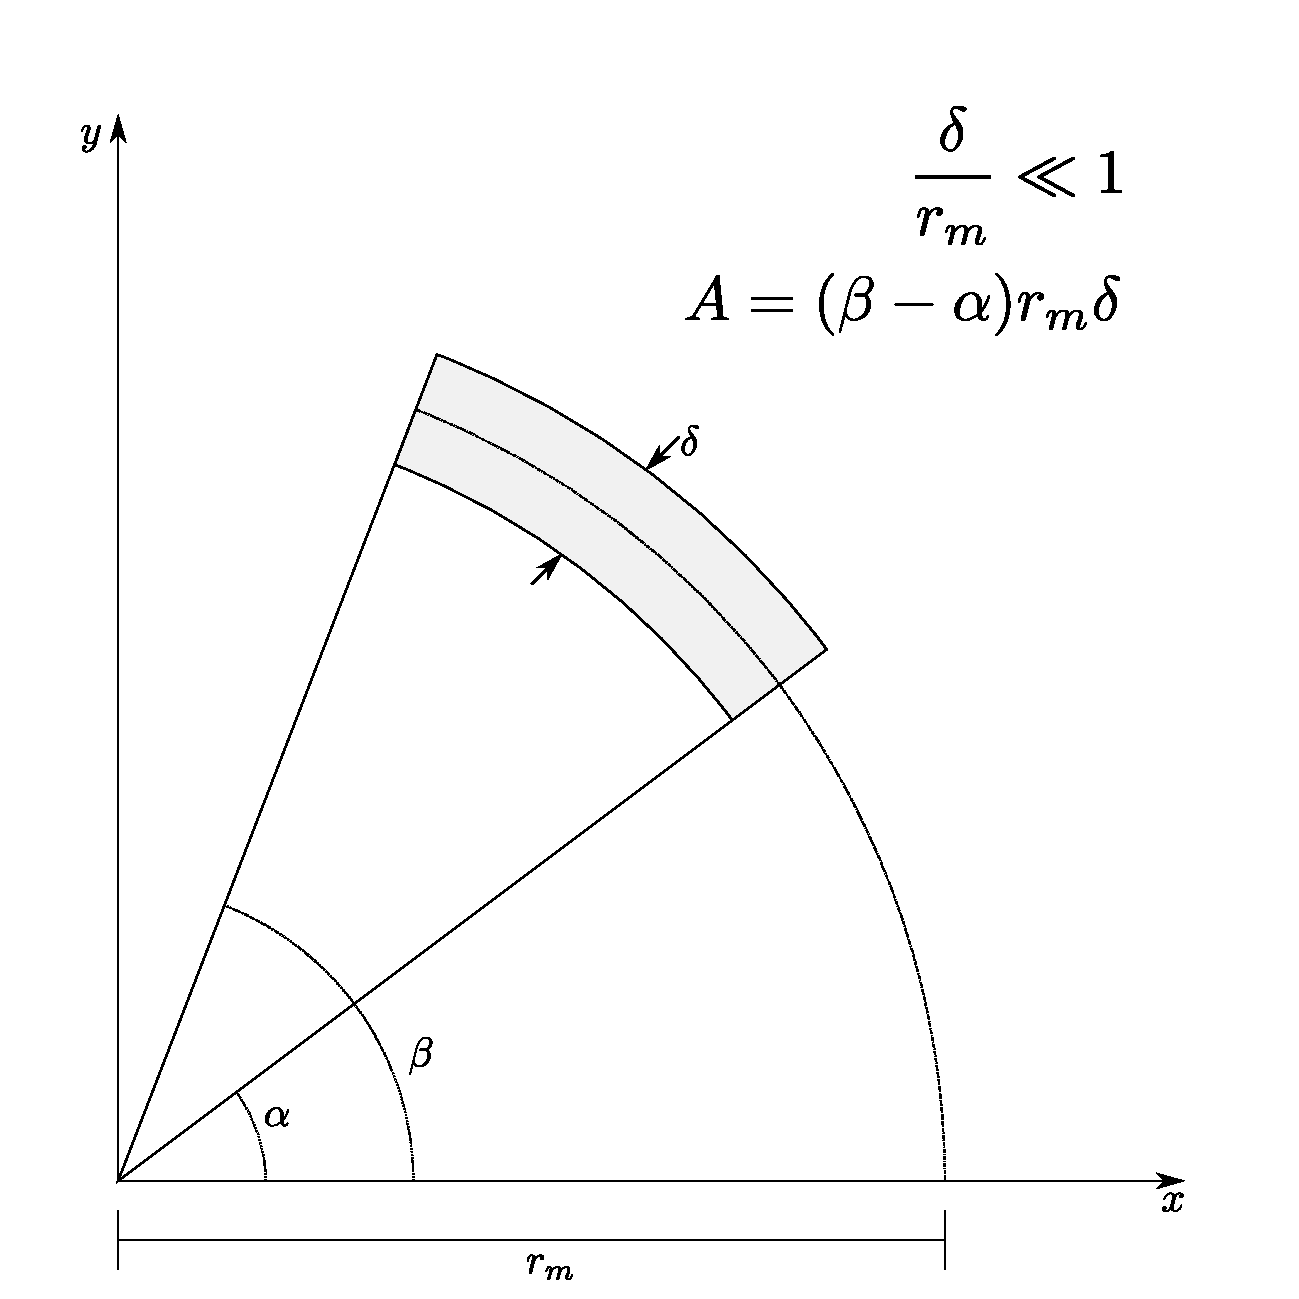
\includegraphics[width=0.75\textwidth]{Immagini/Parte_1/Esercizio1_7/Esercizio1_7.pdf}
\caption{}
\label{Esercizio1_7}
\end{figure}
%----------------------------------------------------------------------------------------

\noindent Possiamo utilizzare i risultati ottenuti nell'Esercizio 1.3 ponendo:
%----------------------------------------------------------------------------------------
\begin{align*}
R_e &= r_m+\frac{\delta}{2} \\
R_i &= r_m-\frac{\delta}{2}
\end{align*}
%----------------------------------------------------------------------------------------
Con semplici calcoli si trova:
%----------------------------------------------------------------------------------------
%----------------------------------------------------------------------------------------
\begin{align*}
R_e^2-R_i^2 &= 2r_m\delta \\
R_e^3-R_i^3 &= \frac{1}{4}(\delta^2+12r_m^2)\delta
\end{align*}
%----------------------------------------------------------------------------------------
e così le formule dell'Esercizio 1.3 divengono:
%----------------------------------------------------------------------------------------
%----------------------------------------------------------------------------------------
\begin{align*}
S_x &= \frac{1}{12}(\delta^2+12r_m^2)(\cos\alpha-\cos\beta)\delta \\
S_y &= \frac{1}{12}(\delta^2+12r_m^2)(\sin\beta-\sin\alpha)\delta
\end{align*}
%----------------------------------------------------------------------------------------
%----------------------------------------------------------------------------------------
\begin{align*}
x_G &= \frac{2}{3}\frac{\frac{1}{4}(\delta^2+12r_m^2)\delta}{2r_m\delta}\frac{\sin\beta-\sin\alpha}{\beta-\alpha} = \frac{1}{12}\frac{\delta^2+12r_m^2}{r_m}\frac{\sin\beta-\sin\alpha}{\beta-\alpha} \\
y_G &= \frac{1}{12}\frac{\delta^2+12r_m^2}{r_m}\frac{\cos\alpha-\cos\beta}{\beta-\alpha}
\end{align*}
%----------------------------------------------------------------------------------------
\begin{equation*}
d_G = \frac{1}{12}\frac{(\delta^2+12r_m^2)}{r_m}\frac{\sin\frac{\beta-\alpha}{2}}{\frac{\beta-\alpha}{2}}
\end{equation*}
%----------------------------------------------------------------------------------------
Tuttavia, se $\frac{\delta}{r_m}\ll1$, è lecito adottare le formule:
%----------------------------------------------------------------------------------------
\begin{align*}
S_x &= r_m^2(\cos\alpha-\cos\beta)\delta \\
S_y &= r_m^2(\sin\beta-\sin\alpha)\delta \\ 
x_G &= r_m\frac{\sin\beta-\sin\alpha}{\beta-\alpha} \\
y_G &= r_m\frac{\cos\alpha-\cos\beta}{\beta-\alpha} \\
d_G &= r_m\frac{\sin\frac{\beta-\alpha}{2}}{\frac{\beta-\alpha}{2}}
\end{align*}
%----------------------------------------------------------------------------------------
nelle quali si è trascurato $\delta^2$ rispetto a $12r_m^3$. 
%----------------------------------------------------------------------------------------

\noindent Vale la pena sottolineare che, nel caso $\frac{\delta}{r_m} = \frac{1}{10}$, l'errore insito nelle suddette formule è pari a:
%----------------------------------------------------------------------------------------
\begin{equation*}
\textup{\textsc{errore}} = \frac{\textup{\textsc{valore esatto}}-\textup{\textsc{valore approssimato}}}{\textup{\textsc{valore esatto}}}
\end{equation*}
%----------------------------------------------------------------------------------------
Quindi: 
%----------------------------------------------------------------------------------------
\begin{equation*}
\epsilon = \frac{\delta^2+12r_m^2-12r_m^2}{\delta^2+12r_m^2} = \frac{1}{1+12\bigl(\frac{r_m}{\delta}\bigr)^2} = \frac{1}{1201} = 0.0008 = 0.08\%
\end{equation*}
%----------------------------------------------------------------------------------------
che, per un ingegnere, \textbf{non è un errore}.
%------------------------------------------------
%%----------------------------------------------------------------------------------------
\part{Momento di inerzia di una figura piana}
\setcounter{section}{0}
\section{Definizione di momento di inerzia}
%\label{paragrafo1-1}
%----------------------------------------------------------------------------------------
Con riferimento alla figura~\vref{figura1-2}, si definisce momento di inerzia rispetto alla retta $r$ la quantità:
%----------------------------------------------------------------------------------------
\begin{equation} \label{equazione2-1}
I_r = \int\int_A \lambda^2dA \tag{2.1}
\end{equation}
%----------------------------------------------------------------------------------------
Nel caso di figura~\ref{figura1-3}, la precedente relazione si particolarizza nelle:
%----------------------------------------------------------------------------------------
\begin{align}
I_x &= \int\int_A y^{2}dA \tag{2.2a} \label{equazione2-2a} \\ 
I_y &= \int\int_A x^{2}dA \tag{2.2b} \label{equazione2-2b}
\end{align}
%----------------------------------------------------------------------------------------
È ovvio che $I_r$ è sempre maggiore di zero ($I_r>0$) e le sue dimensioni fisiche sono $[L^4]$.
%----------------------------------------------------------------------------------------
\section{Formule notevoli di momenti di inerzia}
%----------------------------------------------------------------------------------------
\renewcommand{\thefigure}{2~-~1}
\begin{figure}[ht]
\centering
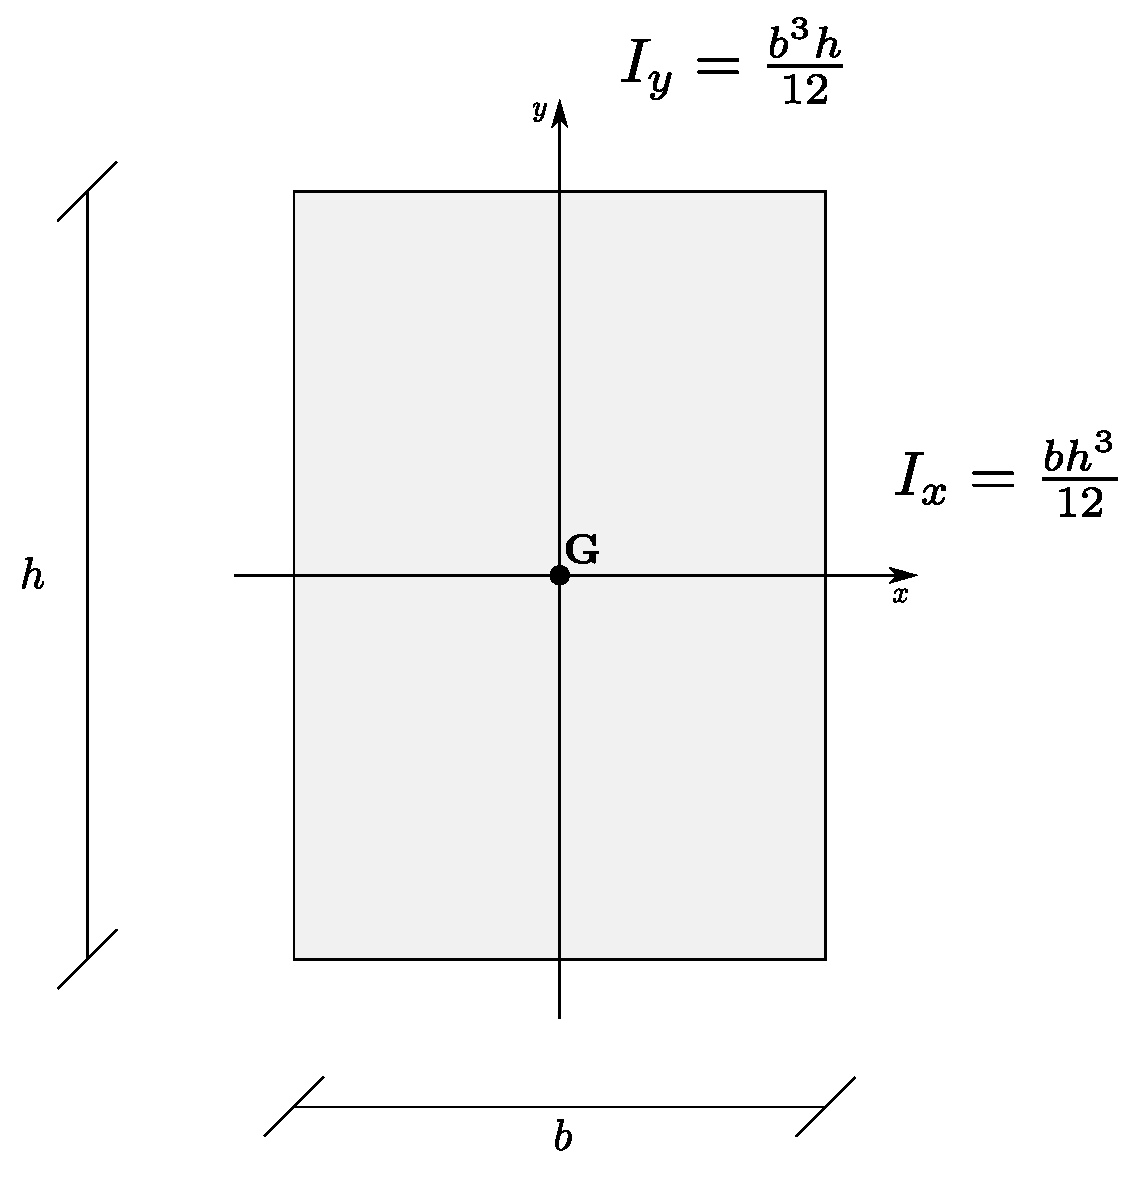
\includegraphics[width=0.55\textwidth]{Immagini/Parte_2/Figura2_1/Figura2_1.pdf}
\caption{}
\label{figura2-1}
\end{figure}
%----------------------------------------------------------------------------------------
%---------------------------------------------------------------------------------------------------------------------------------------------
\begin{align}
I_x &= \frac{bh^{3}}{12} \tag{2.3a} \label{equazione2-3a} \\
I_y &= \frac{b^{3}h}{12} \tag{2.3b} \label{equazione2-3b}
\end{align}
%---------------------------------------------------------------------------------------------------------------------------------------------
Limitiamoci a dimostrare la relazione per il calcolo di $I_x$. 
%----------------------------------------------------------------------------------------
\begin{equation*}
I_x = \int\int_A y^{2}dA = \int_{-\frac{b}{2}}^{+\frac{b}{2}}dx\int_{-\frac{h}{2}}^{+\frac{h}{2}}y^{2}dy = \bigl[x\bigr]_{-\frac{b}{2}}^{+\frac{b}{2}}\cdot \frac{1}{3}\bigl[y^3\bigr]_{-\frac{h}{2}}^{+\frac{h}{2}} = \frac{bh^3}{12}
\end{equation*}
%----------------------------------------------------------------------------------------
%----------------------------------------------------------------------------------------
\renewcommand{\thefigure}{2~-~2}
\begin{figure}[ht]
\centering
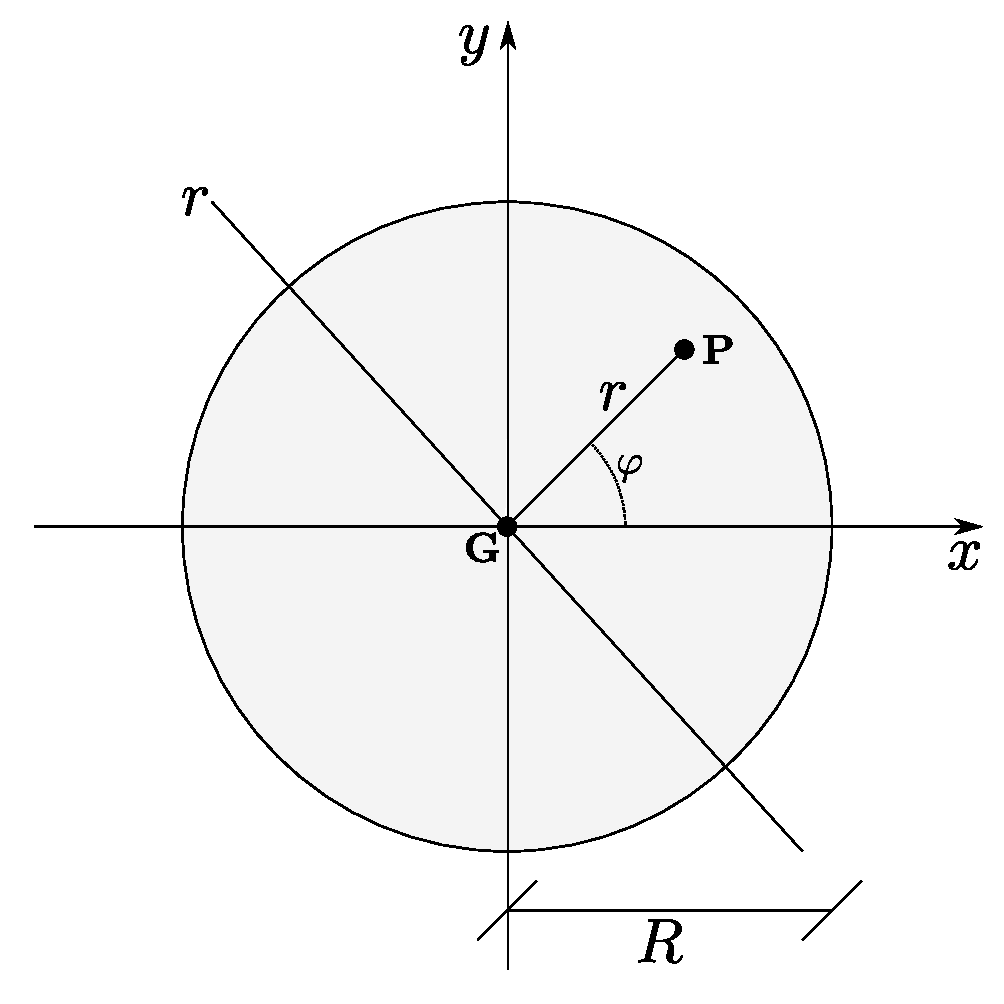
\includegraphics[width=0.58\textwidth]{Immagini/Parte_2/Figura2_2/Figura2_2.pdf}
\caption{}
\label{figura2-2}
\end{figure}
%----------------------------------------------------------------------------------------
È evidente che nel caso di un cerchio
%----------------------------------------------------------------------------------------
\begin{equation*}
I_r = I_x = I_y, \quad \forall r \owns \mathbf{G}
\end{equation*}
%----------------------------------------------------------------------------------------
Dimostreremo che 
%----------------------------------------------------------------------------------------
\begin{equation} \label{equazione2-4}
\boxed{I_x = \frac{\pi R^4}{4}}
\tag{2.4}
\end{equation}
%----------------------------------------------------------------------------------------
\begin{equation*}
I_x = \int\int_A y^{2}dxdy = \int\int_A (r\sin\varphi)^{2}rd\varphi dr = \int_{0}^{R}r^{3}dr\int_{0}^{2\pi}\sin^{2}\varphi d\varphi = \frac{R^4}{4}\biggl[\frac{1}{2}\varphi-\frac{1}{4}\sin 2\varphi \biggr]_{0}^{2\pi}
\end{equation*}
%----------------------------------------------------------------------------------------
che verifica la~\eqref{equazione2-4}.
%----------------------------------------------------------------------------------------
%----------------------------------------------------------------------------------------
\renewcommand{\thefigure}{2~-~3}
\begin{figure}[ht]
\centering
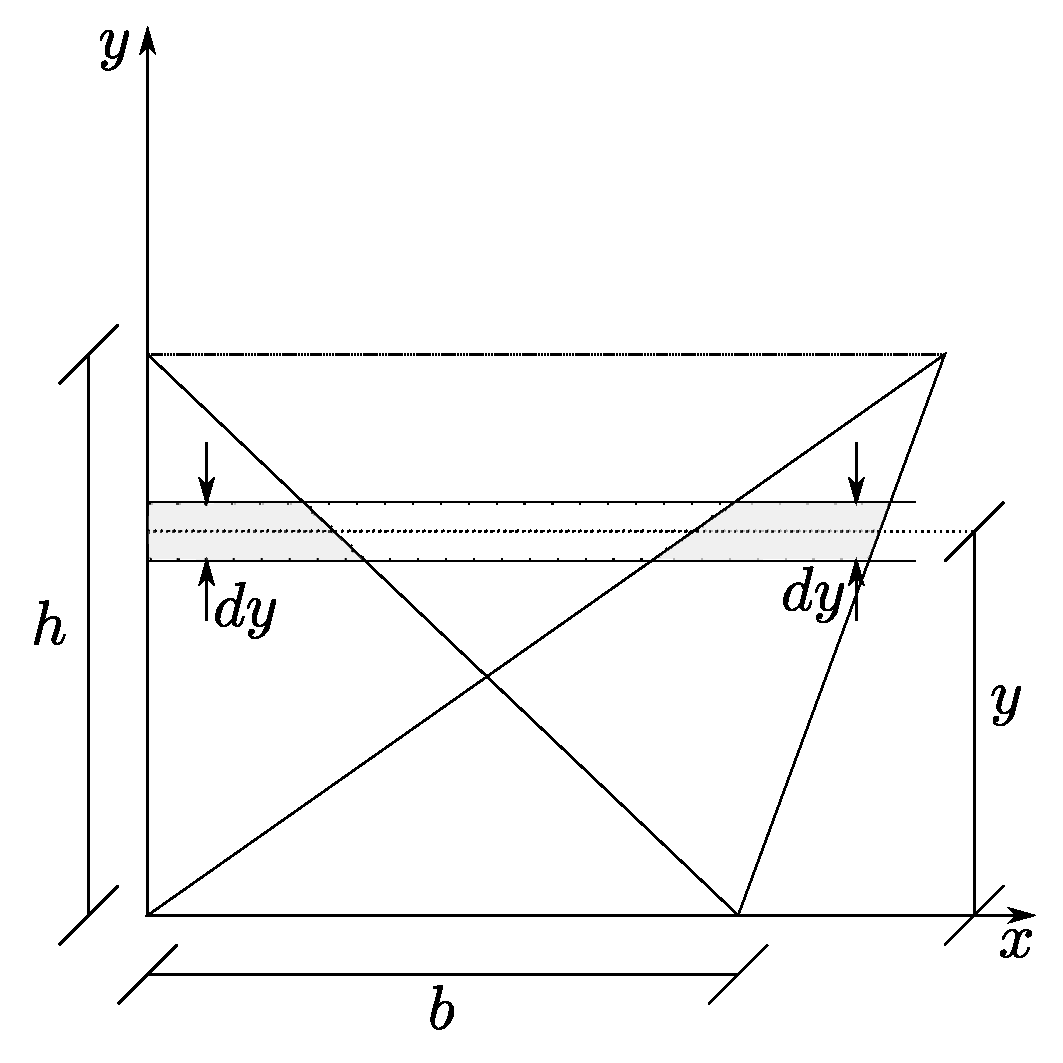
\includegraphics[width=0.75\textwidth]{Immagini/Parte_2/Figura2_3/Figura2_3.pdf}
\caption{}
\label{figura2-3}
\end{figure}
%----------------------------------------------------------------------------------------
\noindent In figura~\ref{figura2-3} sono riportati un triangolo rettangolo ed uno scaleno aventi in comune la base $b$ e l'altezza $h$. È interessante osservare che due striscette ombreggiate di spessore $dy$ hanno, a parità di quota $y$, la stessa lunghezza e quindi la stessa area $dA$. Il momento di inerzia rispetto alla retta coincidente con la base (asse $x$ in figura) è dunque uguale per entrambi. Nel caso del triangolo rettangolo è facile calcolare l'integrale:
%----------------------------------------------------------------------------------------
\begin{equation*}
I_x = \int\int_A y^{2}dxdy
\end{equation*}
%----------------------------------------------------------------------------------------
Si lascia al lettore il compito di verificare che l'equazione~\eqref{equazione2-3a} è valida per qualunque triangolo di altezza $h$ e base $b$, se $x$ coincide con la base.
%----------------------------------------------------------------------------------------

\noindent Per il triangolo rettangolo risulta chiaramente 
%----------------------------------------------------------------------------------------
\begin{equation*}
I_y = \frac{hb^{3}}{12}
\end{equation*}
%----------------------------------------------------------------------------------------
È ovvio che quest'ultima formula non è valida per il triangolo scaleno; per esso sarà certamente $I_y > \frac{hb^{3}}{12}$; e, comunque, impareremo a calcolarlo in seguito. 
%----------------------------------------------------------------------------------------
%----------------------------------------------------------------------------------------
\renewcommand{\thefigure}{2~-~4}
\begin{figure}[ht]
\centering
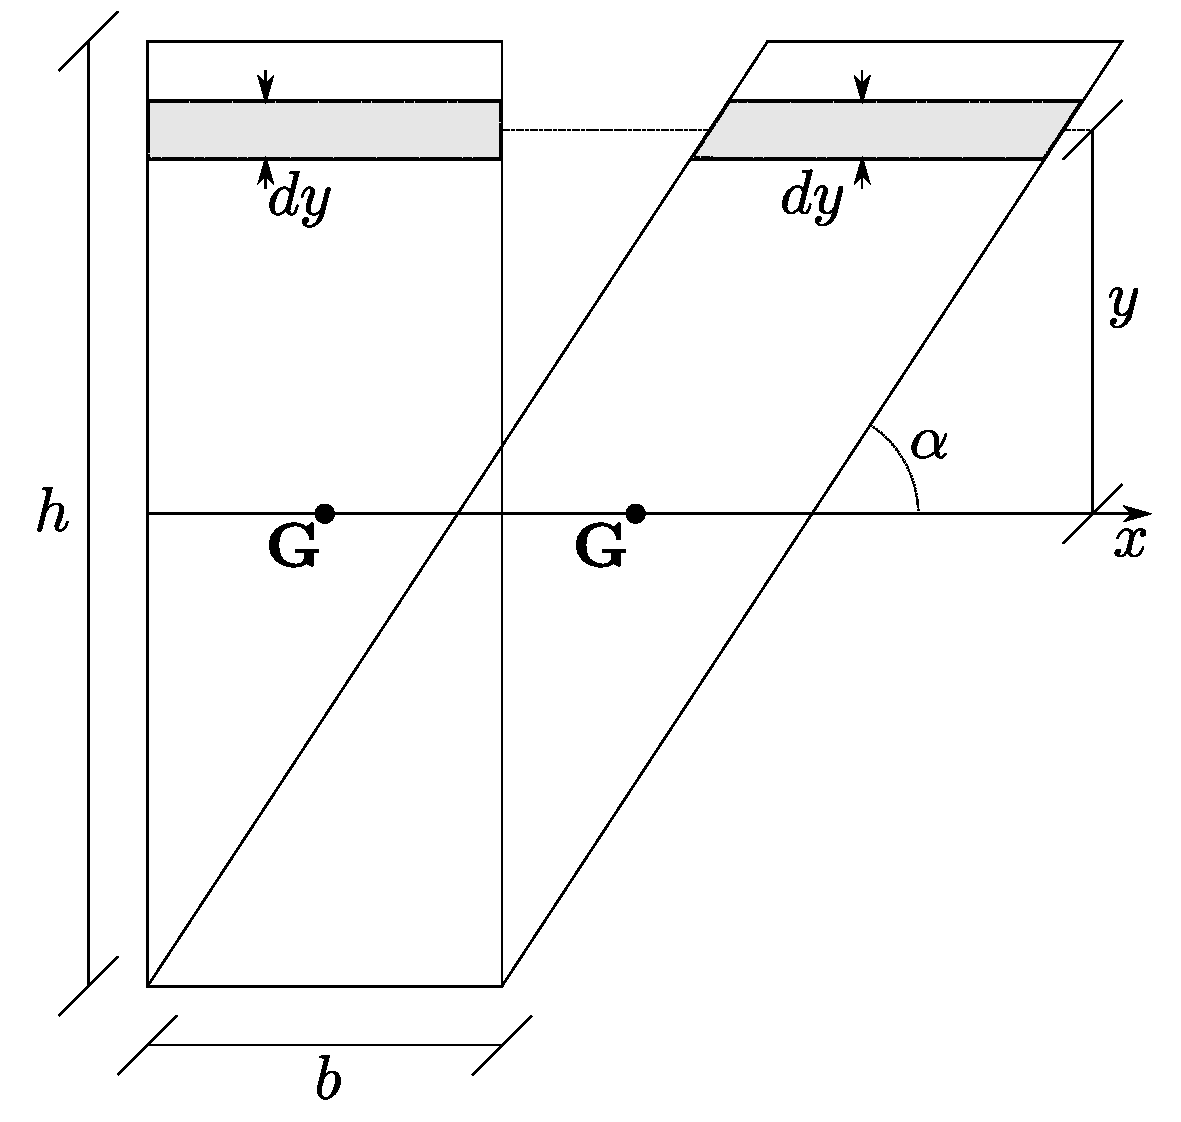
\includegraphics[width=0.75\textwidth]{Immagini/Parte_2/Figura2_4/Figura2_4.pdf}
\caption{}
\label{figura2-4}
\end{figure}
%----------------------------------------------------------------------------------------
\noindent In figura~\ref{figura2-4} sono riportati un rettangolo ed un parallelogramma aventi base ed altezza uguali. È evidente che le due striscette ombreggiate hanno la stessa area $bdy$; il momento di inerzia rispetto ad $x$ è, pertanto, uguale per entrambi. 
%----------------------------------------------------------------------------------------

\noindent Possiamo pertanto affermare che il momento di inerzia di un parallelogramma rispetto all'asse baricentrico parallelo alle basi vale, qualunque sia il valore dell'angolo $\alpha$:
%----------------------------------------------------------------------------------------
\begin{equation*}
I_x = \frac{bh^{3}}{12}
\end{equation*}
%----------------------------------------------------------------------------------------
\section{Momento di inerzia polare}
%----------------------------------------------------------------------------------------
\renewcommand{\thefigure}{2~-~5}
\begin{figure}[ht]
\centering
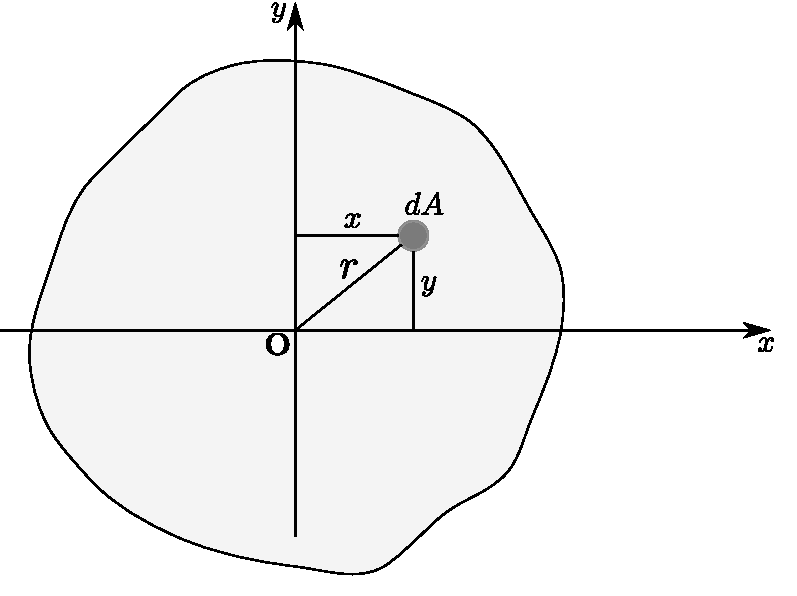
\includegraphics[width=0.75\textwidth]{Immagini/Parte_2/Figura2_5/Figura2_5.pdf}
\caption{}
\label{figura2-5}
\end{figure}
%----------------------------------------------------------------------------------------
In figura~\ref{figura2-5} è rappresentata una figura piana; $\mathbf{O}$ è un punto qualunque ad essa complanare; diciamo $r$ la distanza della generica areola $dA$ dal punto $\mathbf{O}$. 
%----------------------------------------------------------------------------------------

\noindent Si dice momento di inerzia polare della figura rispetto al polo $\mathbf{O}$ la quantità:
%----------------------------------------------------------------------------------------
\begin{equation} \label{equazione2-5}
\boxed{I_x = \int\int_A r^{2}dA}
\tag{2.5}
\end{equation}
%----------------------------------------------------------------------------------------
Presi comunque due assi di riferimento ortogonali con origine in $\mathbf{O}$, sarà ovviamente: 
%----------------------------------------------------------------------------------------
\begin{equation*}
r^2 = x^2 + y^2
\end{equation*}
%----------------------------------------------------------------------------------------
e pertanto la~\eqref{equazione2-5} diviene
%----------------------------------------------------------------------------------------
\begin{equation*}
I_p = \int\int_A (x^2+y^2)dA = \int\int_A x^{2}dA + \int\int_A y^{2}dA
\end{equation*}
%----------------------------------------------------------------------------------------
cioè
%----------------------------------------------------------------------------------------
\begin{equation} \label{equazione2-6}
\boxed{I_p = I_x + I_y}
\tag{2.6}
\end{equation}
%----------------------------------------------------------------------------------------
Ribadiamo che la~\eqref{equazione2-6} è valida comunque si prendano $x$ ed $y$, purché ortogonali e con origine nel polo.
%----------------------------------------------------------------------------------------
\section{Teorema del trasporto del momento di inerzia}
%----------------------------------------------------------------------------------------
\renewcommand{\thefigure}{2~-~6}
\begin{figure}[ht]
\centering
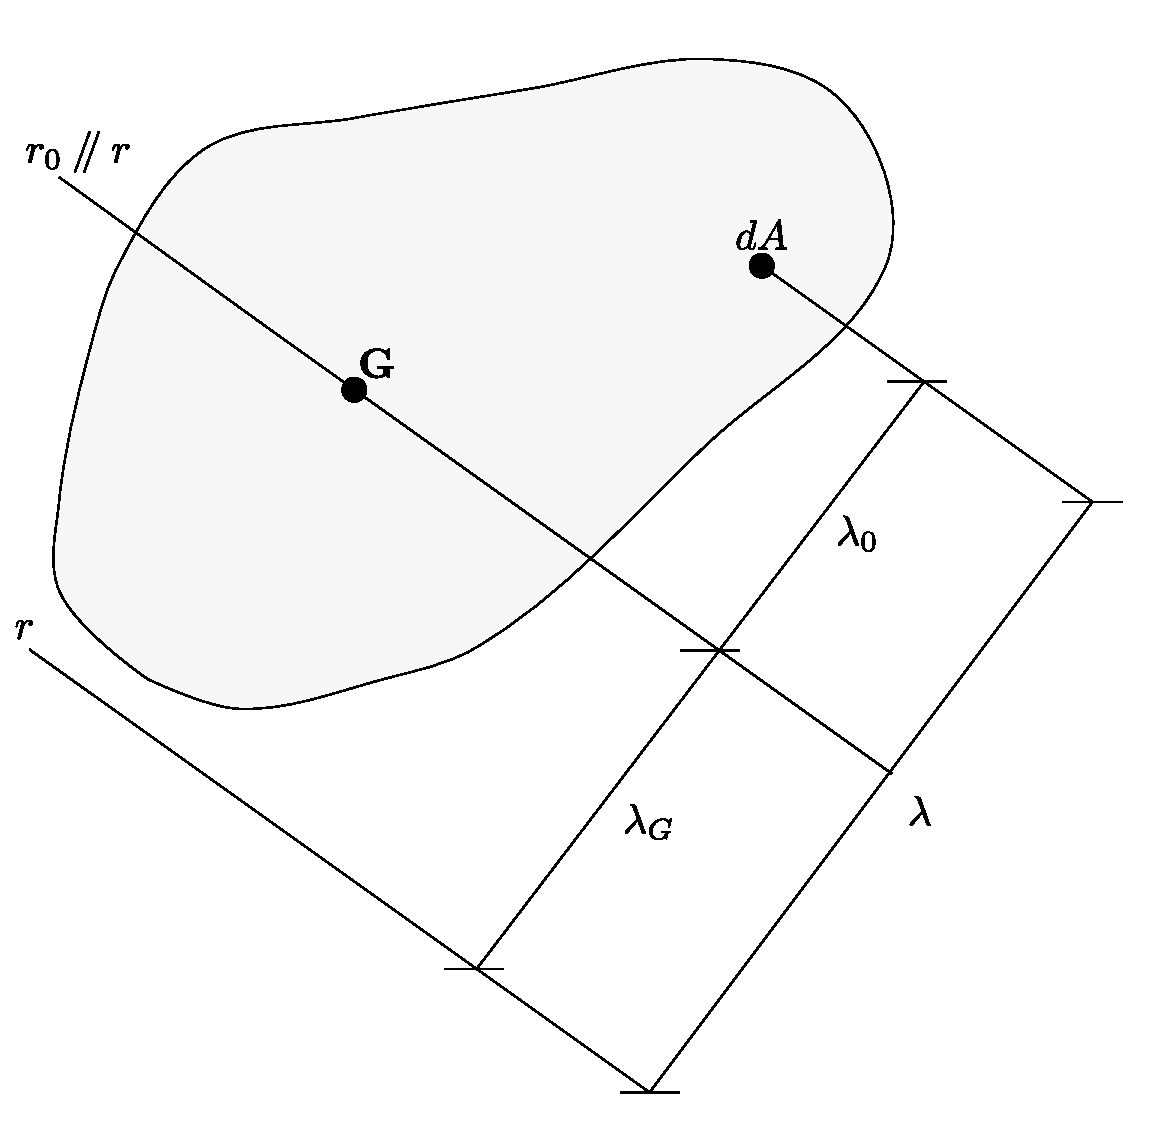
\includegraphics[width=0.75\textwidth]{Immagini/Parte_2/Figura2_6/Figura2_6.pdf}
\caption{}
\label{figura2-6}
\end{figure}
%----------------------------------------------------------------------------------------
%----------------------------------------------------------------------------------------
Dimostreremo che, qualunque, sia la figura piana e qualunque sia la retta $r$, vale la relazione:
%----------------------------------------------------------------------------------------
\begin{equation} \label{equazione2-7}
\boxed{I_r = I_{r_0}+A\lambda_{G}^{2}}
\tag{2.7}
\end{equation}
%----------------------------------------------------------------------------------------
La~\eqref{equazione2-7} esprime il \textsc{Teorema di Huygens}; il termine $A\lambda_{G}^{2}$ è detto \emph{termine di trasporto}. Per dimostrare la~\eqref{equazione2-7} cominciamo ad osservare che, come è evidente in figura~\ref{figura2-6}, risulta:
%----------------------------------------------------------------------------------------
\begin{equation*}
\lambda = \lambda_0+\lambda_G
\end{equation*}
%----------------------------------------------------------------------------------------
Ciò premesso
%----------------------------------------------------------------------------------------
\begin{equation*}
I_r = \int\int_A \lambda^{2}dA = \int\int_A (\lambda_0+\lambda_G)^{2}dA = \int\int_A \lambda_{0}^{2}dA + \int\int_A \lambda_{G}^{2}dA + \int\int_A 2\lambda_{0}\lambda_{G}dA
\end{equation*}
%----------------------------------------------------------------------------------------
Essendo $\lambda_G=\textup{\textsc{costante}}$
%----------------------------------------------------------------------------------------
\begin{equation*}
I_r = \int\int_A \lambda_{0}^{2}dA + \lambda_{G}^{2}\int\int_AdA + 2\lambda_{G}\int\int_A \lambda_{0}dA
\end{equation*}
%----------------------------------------------------------------------------------------
Ovviamente risulta 
%----------------------------------------------------------------------------------------
\begin{align*}
\int\int_A dA &= A \\
\int\int_A \lambda_{0}^{2}dA &= I_{r_0} \\
\int\int_A \lambda_{0}dA &= S_{r_0} = 0\,\,\textup{essendo}\,\,r_0\,\owns\,\mathbf{G}
\end{align*}
%----------------------------------------------------------------------------------------
e così si perviene alla~\eqref{equazione2-7}.
%----------------------------------------------------------------------------------------
\section{Altre formule notevoli di momento di inerzia}
%----------------------------------------------------------------------------------------
\renewcommand{\thefigure}{2~-~7}
\begin{figure}[ht]
\centering
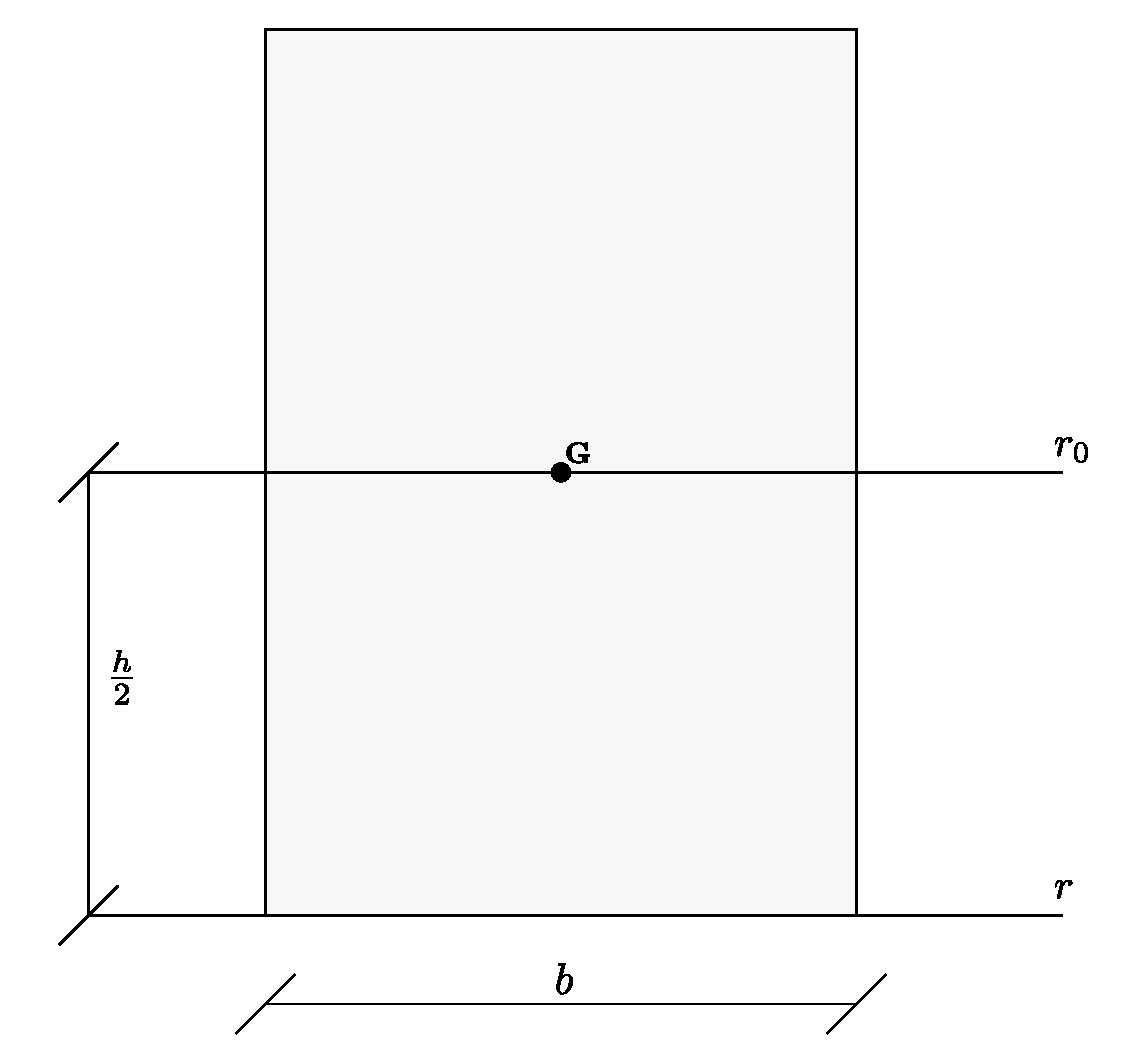
\includegraphics[width=0.75\textwidth]{Immagini/Parte_2/Figura2_7/Figura2_7.pdf}
\caption{}
\label{figura2-7}
\end{figure}
%----------------------------------------------------------------------------------------
%----------------------------------------------------------------------------------------
Con riferimento al rettangolo di figura~\ref{figura2-7} vogliamo calcolare $I_r$. Applicando il teorema del trasporto: 
%----------------------------------------------------------------------------------------
\begin{equation*}
I_r = I_{r_0}+A\lambda_{G}^{2} = \frac{bh^{3}}{12}+bh\biggl(\frac{h}{2}\biggr)^2
\end{equation*}
%----------------------------------------------------------------------------------------
e semplificando 
%----------------------------------------------------------------------------------------
\begin{equation} \label{equazione2-8}
\boxed{I_r = \frac{bh^{3}}{3}}
\tag{2.8}
\end{equation}
%----------------------------------------------------------------------------------------
%----------------------------------------------------------------------------------------
\renewcommand{\thefigure}{2~-~8}
\begin{figure}[ht]
\centering
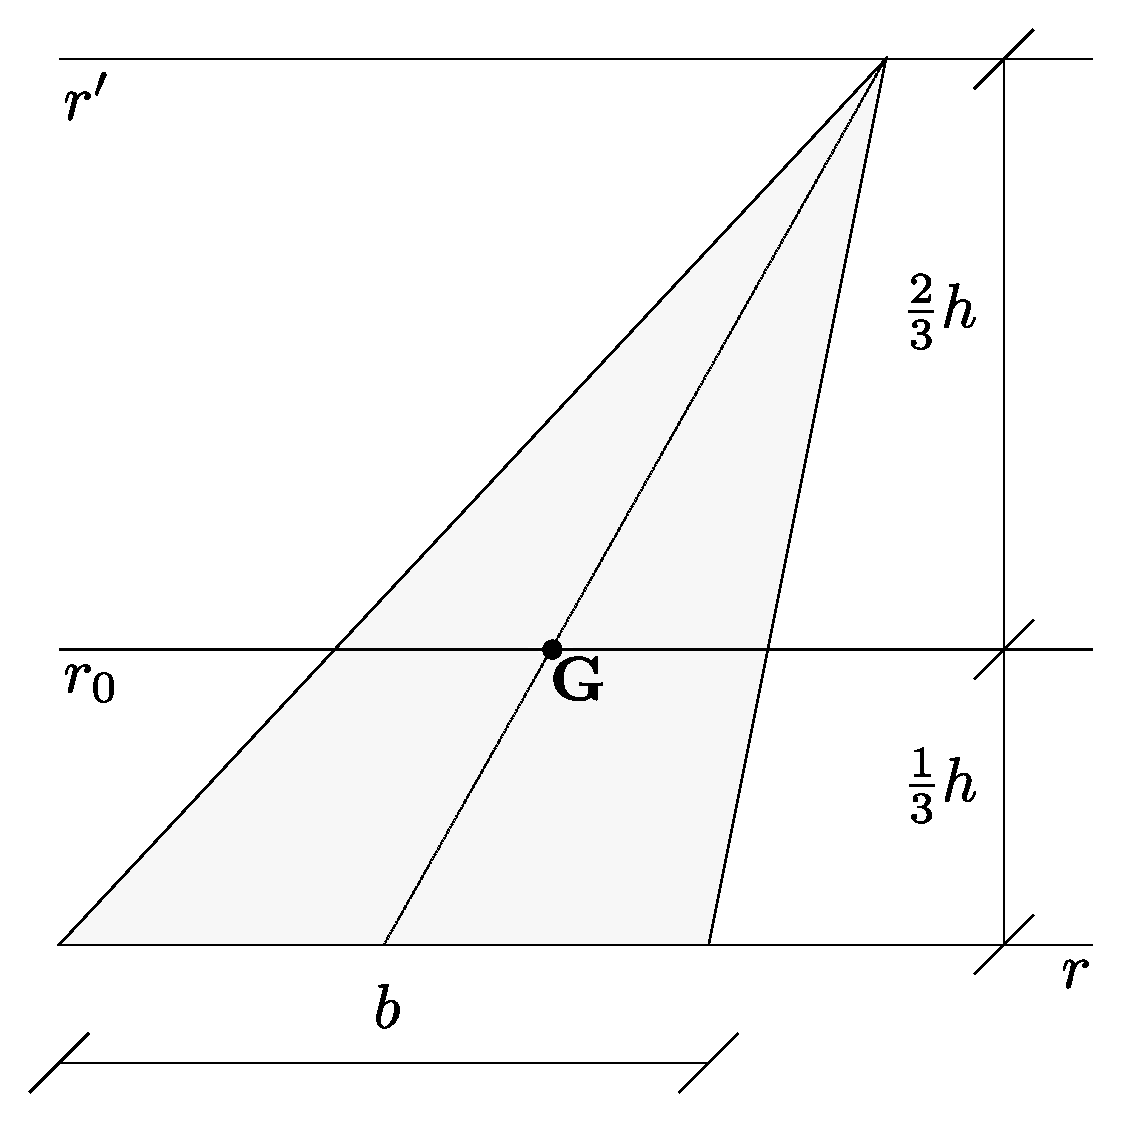
\includegraphics[width=0.75\textwidth]{Immagini/Parte_2/Figura2_8/Figura2_8.pdf}
\caption{}
\label{figura2-8}
\end{figure}
%----------------------------------------------------------------------------------------
Con riferimento al triangolo di figura~\ref{figura2-8} è noto che 
%----------------------------------------------------------------------------------------
\begin{equation*}
I_r = \frac{bh^{3}}{12}
\end{equation*}
%----------------------------------------------------------------------------------------
Ci proponiamo di calcolare $I_{r_0}$ ed $I_{r'}$. 
%----------------------------------------------------------------------------------------

\noindent Utilizzeremo, ovviamente, il teorema del trasporto:
%----------------------------------------------------------------------------------------
\begin{equation*}
I_{r_0} = I_r - A\lambda_{G}^{2} = \frac{bh^{3}}{12}-\frac{bh}{2}\biggl(\frac{h}{3}\biggr)^2
\end{equation*}
%----------------------------------------------------------------------------------------
semplificando
%----------------------------------------------------------------------------------------
\begin{equation}
\boxed{I_{r_0} = \frac{bh^{3}}{36}}
\end{equation}
%----------------------------------------------------------------------------------------
E ancora 
%----------------------------------------------------------------------------------------
\begin{equation*}
I_{r_0} = I_{r'} + A\lambda_{G}^{2} = \frac{bh^{3}}{36}+\frac{bh}{2}\biggl(\frac{2}{3}h\biggr)^2
\end{equation*}
%----------------------------------------------------------------------------------------
semplificando
%----------------------------------------------------------------------------------------
\begin{equation*}
\boxed{I_{r'} = \frac{bh^{3}}{4}}
\end{equation*}
%----------------------------------------------------------------------------------------
\clearpage
\section{Esercizi}
\paragraph{Esercizio 2.1}
Calcolare $I_y$ per il triangolo \textsc{abc} riportato in figura
%----------------------------------------------------------------------------------------
\renewcommand{\thefigure}{2.1~-~1}
\begin{figure}[ht]
\centering
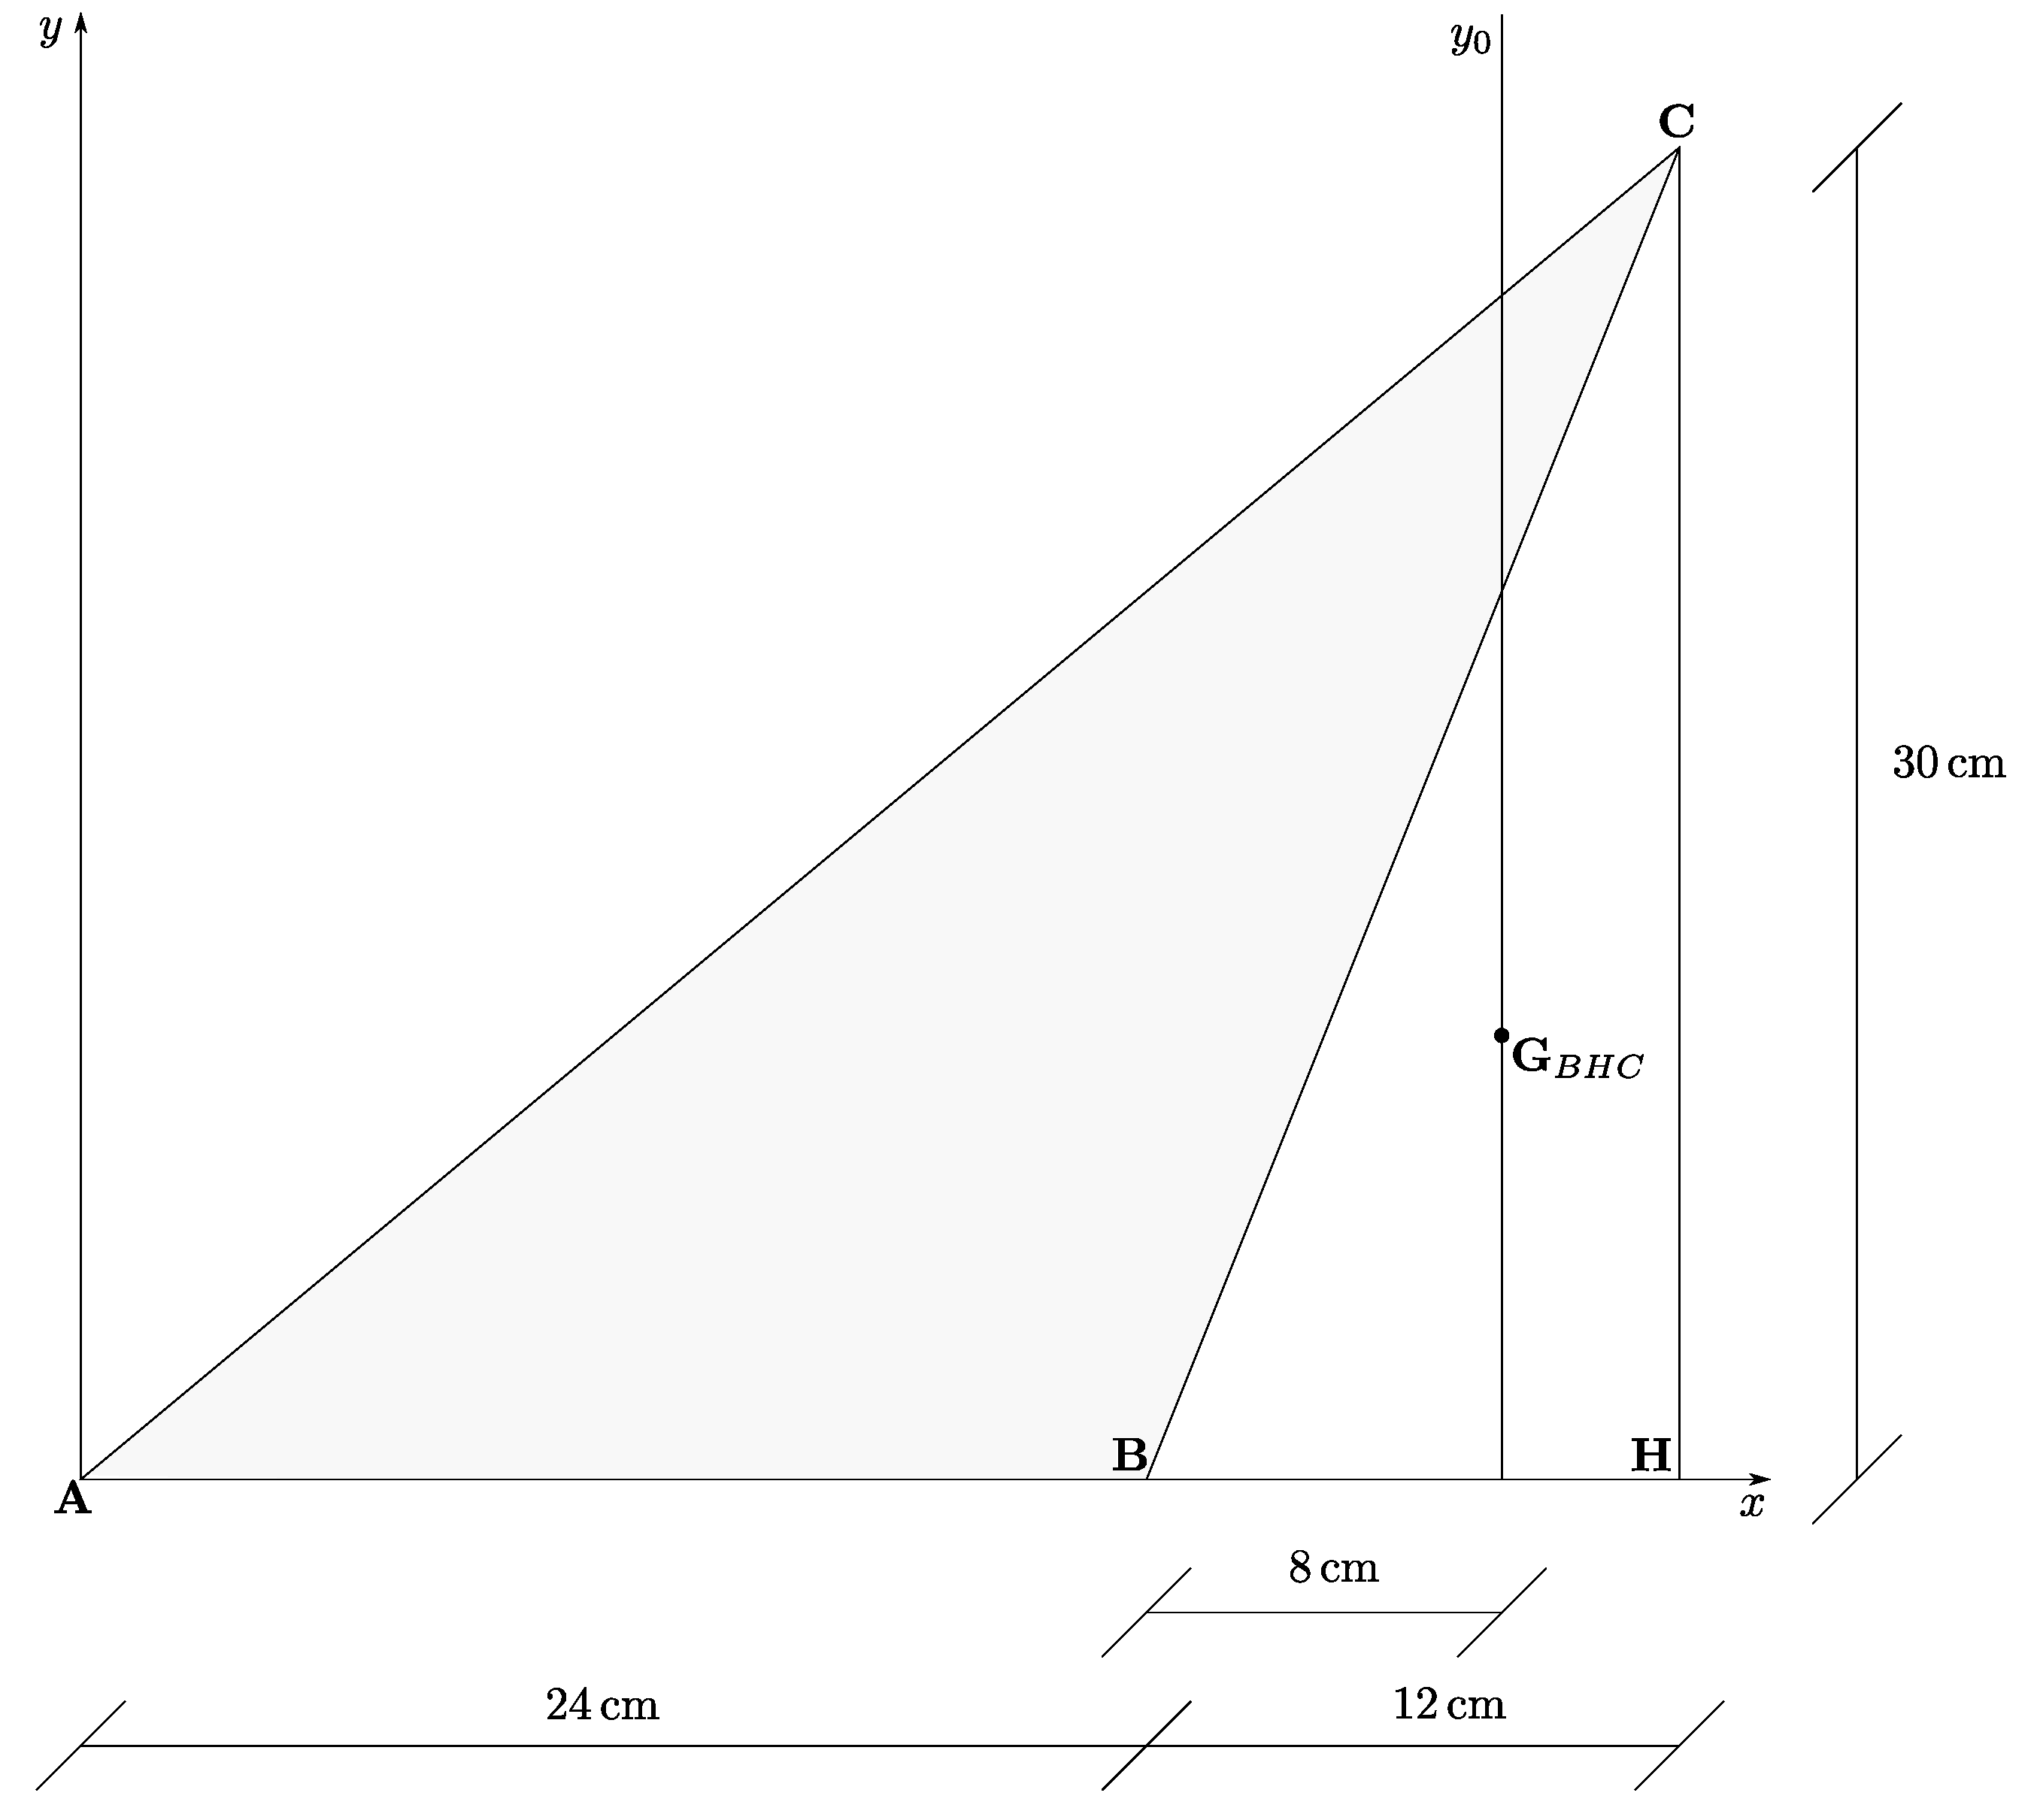
\includegraphics[width=0.95\textwidth]{Immagini/Parte_2/Esercizio2_1/Esercizio2_1_1.pdf}
\caption{}
\label{Esercizio2_1}
\end{figure}
%----------------------------------------------------------------------------------------

\noindent Chiaramente, si può porre 
%----------------------------------------------------------------------------------------
\begin{equation*}
(I_{y})_{ABC} = (I_{y})_{AHC}-(I_{y})_{BHC}
\end{equation*}
%----------------------------------------------------------------------------------------
Calcoliamo, dunque, $(I_{y})_{AHC}$ e $(I_{y})_{BHC}$:
%----------------------------------------------------------------------------------------
\begin{align*}
(I_{y})_{AHC} &= \frac{30\times 36^3}{4} = 349920\,\textup{cm}^4 \\
(I_{y})_{BHC} &= (I_{y_0})_{BHC}+A_{BHC}\times \lambda_{G}^{2} = \frac{30\times 12^3}{36}+\frac{30\times 12}{2}\times 32^2 = 185760\,\textup{cm}^4
\end{align*}
%----------------------------------------------------------------------------------------
In definitiva
%----------------------------------------------------------------------------------------
\begin{equation*}
(I_{y})_{ABC} = 349920-185760 = 164160\,\textup{cm}^4
\end{equation*}
%----------------------------------------------------------------------------------------
\clearpage
\paragraph{Esercizio 2.2}
Con riferimento alla figura piana qui rappresentata, si chiede:
%----------------------------------------------------------------------------------------
\begin{enumerate}
\item di determinare $\mathbf{G}$
\item di calcolare $I_r$
\item di calcolare $I_{r_0}$, essendo $r_0$ la retta per $\mathbf{G}$ parallela ad $r$
\end{enumerate}
%----------------------------------------------------------------------------------------
\renewcommand{\thefigure}{2.2~-~1}
\begin{figure}[ht]
\centering
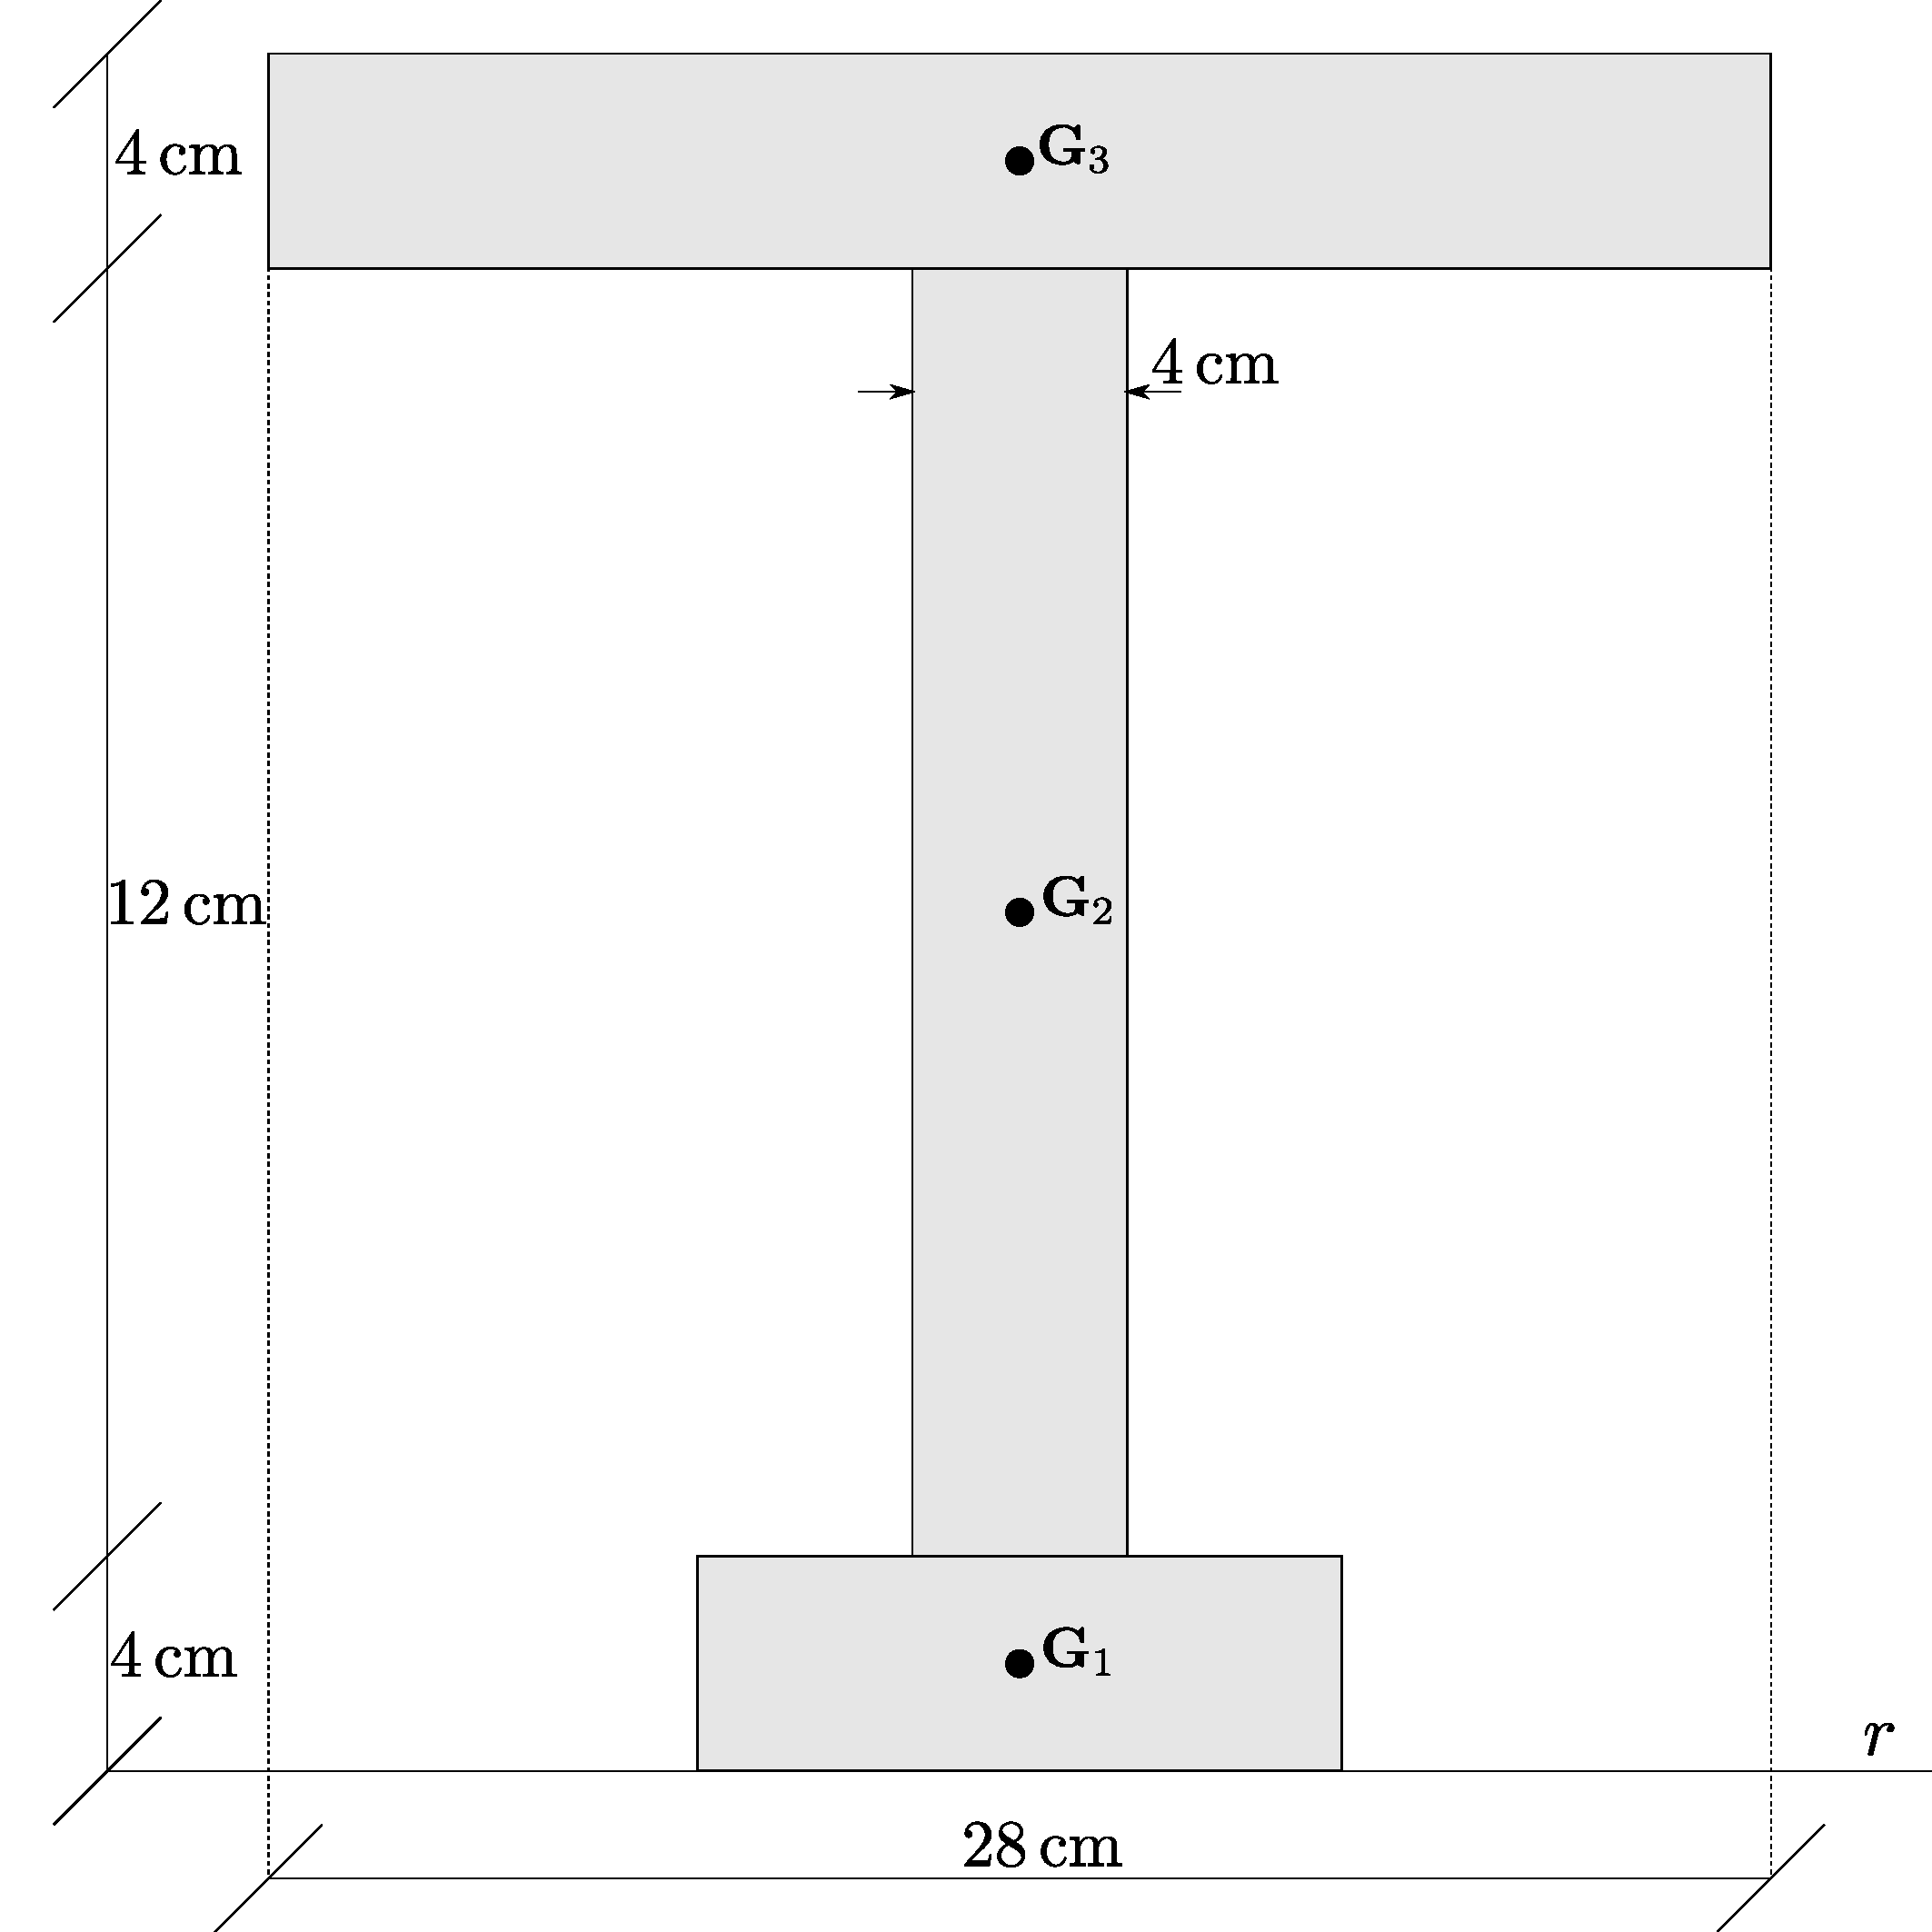
\includegraphics[width=0.95\textwidth]{Immagini/Parte_2/Esercizio2_2/Esercizio2_2_1.pdf}
\caption{}
\label{Esercizio2_1}
\end{figure}
%----------------------------------------------------------------------------------------
\noindent
\subparagraph{Quesito 1:} Il baricentro appartiene, ovviamente, all'asse di simmetria; e, perciò basterà, per determinarlo, calcolare la sua distanza da $r$.
%----------------------------------------------------------------------------------------
\begin{equation*}
\begin{aligned}
A_1 &= 12\times 4 = 48\,\textup{cm}^2 \\
A_2 &= 24\times 4 = 96\,\textup{cm}^2 \\
A_3 &= 28\times 4 = 112\,\textup{cm}^2
\end{aligned}
\,\,\Biggr\}\,\, A = 48+96+112 = 256\,\textup{cm}^2
\end{equation*}
%----------------------------------------------------------------------------------------
\begin{equation*}
\begin{aligned}
S_{1r} &= 48\times 2 = 96\,\textup{cm}^3 \\
S_{2r} &= 96\times 16 = 1536\,\textup{cm}^3 \\
S_{3r} &= 112\times 30  = 3360\,\textup{cm}^3
\end{aligned}
\,\,\Biggr\}\,\, S_r = 96+1536+3360 = 4992\,\textup{cm}^3
\end{equation*}
%----------------------------------------------------------------------------------------
\begin{equation*}
\lambda_G = \frac{S_r}{A} = \frac{4992}{256} = 19.5\,\textup{cm}
\end{equation*}
%----------------------------------------------------------------------------------------
\subparagraph{Quesito 2:} 
%----------------------------------------------------------------------------------------
\begin{equation*}
\begin{aligned}
I_{1r} &= \frac{12\times 4^{3}}{3} = 256\,\textup{cm}^4 \\
I_{2r} &= \frac{4\times 24^{3}}{12}+96\times 16^2 = 29184\,\textup{cm}^4 \\
I_{3r} &= \frac{28\times 4^{3}}{12}+112\times 30^2  = 100949\,\textup{cm}^4
\end{aligned}
\,\,\Biggr\}\,\, I_r = 256+29184+100949 = 130389\,\textup{cm}^4
\end{equation*}
%----------------------------------------------------------------------------------------
\subparagraph{Quesito 3:}
%----------------------------------------------------------------------------------------
\begin{equation*}
I_{r_0} = I_r -A\times \lambda_{G}^{2} = 130389-256\times 19.5^2 = 33045\,\textup{cm}^4
\end{equation*}
%----------------------------------------------------------------------------------------
\clearpage
\paragraph{Esercizio 2.3}
%----------------------------------------------------------------------------------------

\noindent Formulare i momenti di inerzia per il settore di corona circolare dell'Esercizio 1.3. 
%----------------------------------------------------------------------------------------
\newline

\noindent Calcoleremo gli integrali 
%----------------------------------------------------------------------------------------
\begin{align*}
I_x &= \int\int_A y^{2}dxdy \\
I_y &= \int\int_A x^{2}dxdy
\end{align*}
%----------------------------------------------------------------------------------------
Passando alle coordinate polari
%----------------------------------------------------------------------------------------
\begin{equation*}
\,\,\Biggr\{\,\, 
\begin{aligned}
x &= r\cos\varphi \\
y &= r\sin\varphi 
\end{aligned}
\quad ; \quad \lvert\, J \,\lvert = r
\end{equation*}
%----------------------------------------------------------------------------------------
si trova
%----------------------------------------------------------------------------------------
\begin{align*}
I_x &= \int\int_A r^{2}\sin^{2}\varphi rdrd\varphi = \int_{R_i}^{R_e}r^{3}dr\int_{\alpha}^{\beta}\sin^{2}\varphi d\varphi \\
I_y &= \int\int_A r^{2}\cos^{2}\varphi rdrd\varphi = \int_{R_i}^{R_e}r^{3}dr\int_{\alpha}^{\beta}\cos^{2}\varphi d\varphi
\end{align*}
%----------------------------------------------------------------------------------------
Sviluppando gli integrali si trova, infine
%----------------------------------------------------------------------------------------
\begin{align*}
I_x &= \frac{R_{e}^{4}-R_{i}^{4}}{16}(2\beta-2\alpha-\sin 2\beta+\sin 2\alpha)  \\
I_y &= \frac{R_{e}^{4}-R_{i}^{4}}{16}(2\beta-2\alpha-\sin 2\beta+\sin 2\alpha)
\end{align*}
%----------------------------------------------------------------------------------------
Le suddette formule si adattano immediatamente al caso del settore circolare ponendo in esse $R_e = R$ ed $R_i=0$.
%----------------------------------------------------------------------------------------
\clearpage
\paragraph{Esercizio 2.4}
%----------------------------------------------------------------------------------------
Formulare i momenti di inerzia per il settore di corona circolare (di spessore molto sottile) già considerato nell'Esercizio 1.7.
%----------------------------------------------------------------------------------------
\newline

\noindent Cominciamo a porre, nelle due formule di $I_x$ ed $I_y$ trovate nell'esercizio precedente 
%----------------------------------------------------------------------------------------
\begin{align*}
R_e &= r_m +\frac{\delta}{2} \\
R_i &= r_m - \frac{\delta}{2}
\end{align*}
%----------------------------------------------------------------------------------------
Osserviamo intanto che 
%----------------------------------------------------------------------------------------
\begin{equation*}
R_{e}^{4}-R_{i}^{4} = (R_{e}^{2}+R_{i}^{2})(R_{e}^{2}-R_{i}^{2}) = \Bigl(2r_{m}^{2}+\frac{\delta^2}{2}\Bigr)(2r_{m}\delta) = r_{m}\delta(4r_{m}^{2}+\delta^2)
\end{equation*}
%----------------------------------------------------------------------------------------
E quindi
%----------------------------------------------------------------------------------------
\begin{align*}
I_x &= \frac{r_{m}\delta(4r_{m}^{2}+\delta^2)}{16}(2\beta-2\alpha-\sin 2\beta+\sin 2\alpha)  \\
I_y &= \frac{r_{m}\delta(4r_{m}^{2}+\delta^2)}{16}(2\beta-2\alpha-\sin 2\beta+\sin 2\alpha)
\end{align*}
%----------------------------------------------------------------------------------------
E, trascurando $\delta^2$ rispetto a $4r_{m}^{2}$ 
%----------------------------------------------------------------------------------------
%----------------------------------------------------------------------------------------
\begin{align*}
I_x &= \frac{r_{m}^{3}\delta}{4}(2\beta-2\alpha-\sin 2\beta+\sin 2\alpha)  \\
I_y &= \frac{r_{m}^{3}\delta}{4}(2\beta-2\alpha-\sin 2\beta+\sin 2\alpha)
\end{align*}
%----------------------------------------------------------------------------------------
Nel caso $\frac{\delta}{r_m} = \frac{1}{10}$, utilizzando queste due formule, si commette un errore un po' minore dello $0.25\%$.
%----------------------------------------------------------------------------------------
\clearpage
\paragraph{Esercizio 2.5} Calcolare $I_x$ ed $I_y$ per la figura piana riportata qui rappresentata.
%----------------------------------------------------------------------------------------
\renewcommand{\thefigure}{2.5~-~1}
\begin{figure}[h]
\centering
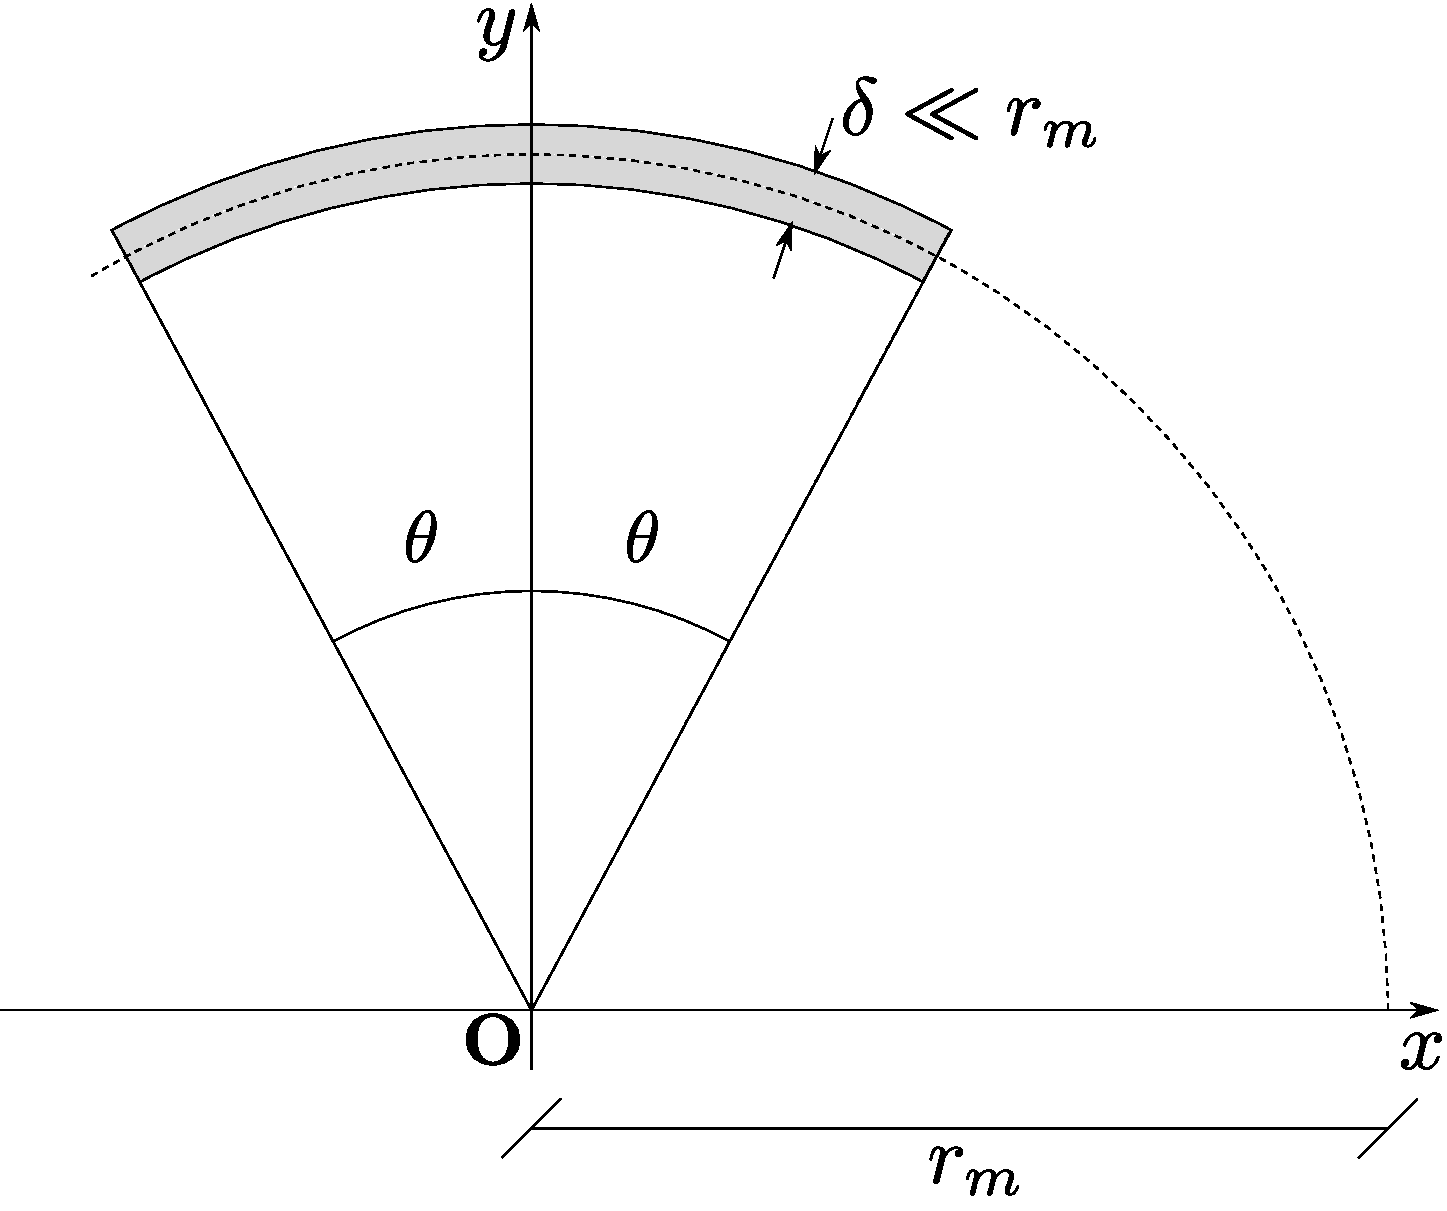
\includegraphics[width=0.85\textwidth]{Immagini/Parte_2/Esercizio2_5/Esercizio2_5_1.pdf}
\caption{}
\label{Esercizio2_5}
\end{figure}
%----------------------------------------------------------------------------------------
%----------------------------------------------------------------------------------------
\newline

\noindent Basta porre, nelle formule approssimate dell'esercizio precedente 
%----------------------------------------------------------------------------------------
\begin{align*}
\alpha &= \frac{\pi}{2} - \theta \\ 
\beta &= \frac{\pi}{2} + \theta
\end{align*}
%----------------------------------------------------------------------------------------
E così
%----------------------------------------------------------------------------------------
\begin{align*}
2\beta-2\alpha &= \pi+2\theta-(\pi-2\theta) = 4\theta \\
\sin 2\beta &= \sin(\pi+2\theta) = -\sin 2\theta \\ 
\sin 2\alpha &= \sin(\pi-2\theta) = \sin 2\theta
\end{align*}
%----------------------------------------------------------------------------------------
Pertanto
%----------------------------------------------------------------------------------------
\begin{align*}
I_x &= \frac{r_{m}^{3}\delta}{2}(2\theta+\sin 2\theta) \\ 
I_y &= \frac{r_{m}^{3}\delta}{2}(2\theta-\sin 2\theta)
\end{align*}
%----------------------------------------------------------------------------------------
%----------------------------------------------------------------------------------------
%----------------------------------------------------------------------------------------
%----------------------------------------------------------------------------------------
%----------------------------------------------------------------------------------------
%----------------------------------------------------------------------------------------
%----------------------------------------------------------------------------------------
%------------------------------------------------
\pagestyle{fancy}
\part{Momento centrifugo}
\setcounter{section}{0}
\section{La definizione di momento centrifugo}
%--------------------------------------------------------------------------------------------------------------------------------------------------------------
\renewcommand{\thefigure}{3~-~1}
\begin{figure}[ht]
\centering
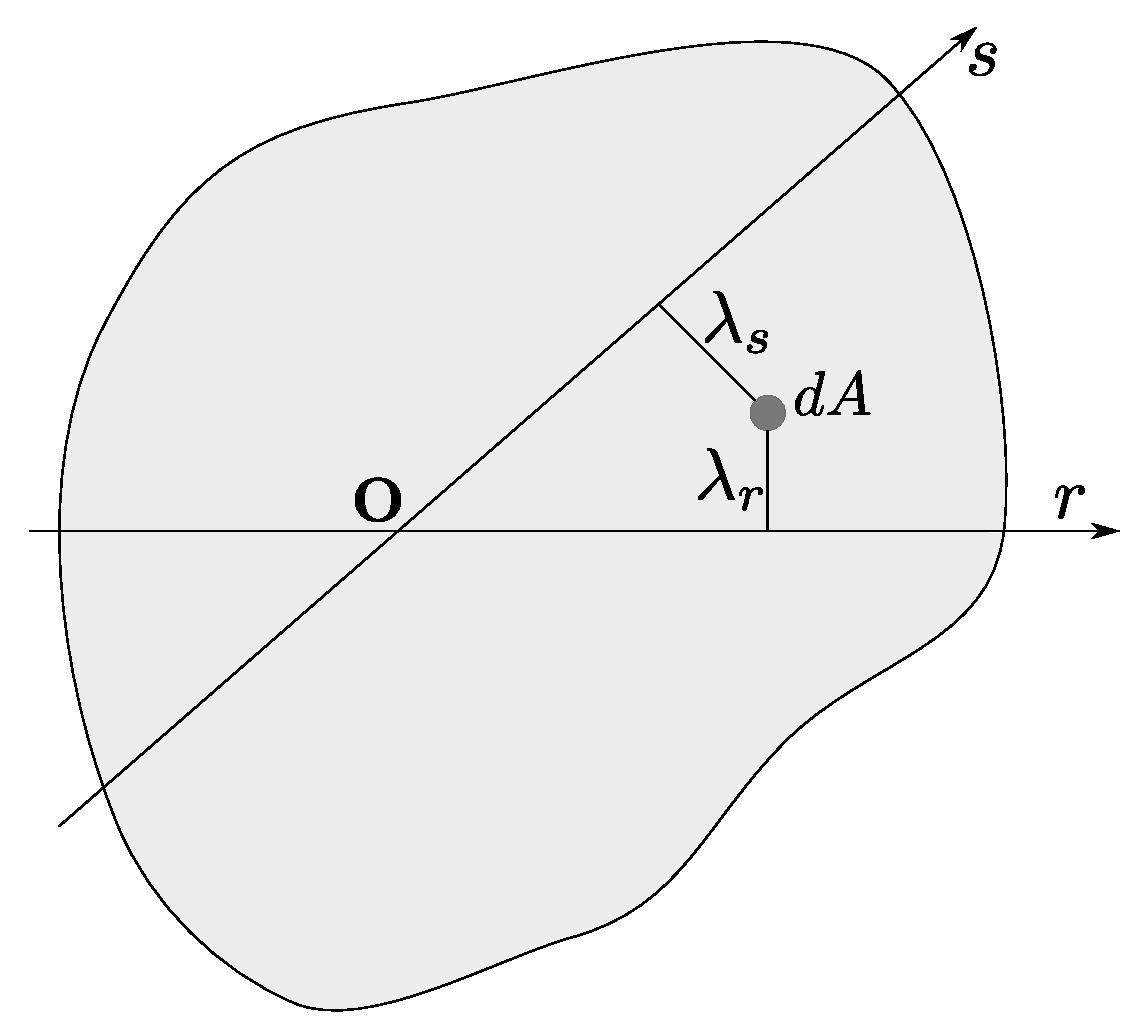
\includegraphics[width=0.55\textwidth]{Immagini/Parte_3/Figura3_1/Figura3_1.pdf}
\caption{}
\label{figura3-1}
\end{figure}
%--------------------------------------------------------------------------------------------------------------------------------------------------------------
Con riferimento alla figura~\ref{figura3-1} si dice momento centrifugo della figura piana rispetto alle rette \textsc{orientate} $r$ ed $s$ la quantità
%--------------------------------------------------------------------------------------------------------------------------------------------------------------
\begin{equation} \label{equazione3-1}
\boxed{I_{rs}=\int\int_A \lambda_{r}\lambda_{s}dA} \tag{3.1}
\end{equation}
%--------------------------------------------------------------------------------------------------------------------------------------------------------------
È evidente che può essere $I_{rs}$ maggiore o minore di zero e che le sue dimensioni fisiche sono $[L^4]$. Rispetto agli assi cartesiani il momento centrifugo si esprime, ovviamente, come
%--------------------------------------------------------------------------------------------------------------------------------------------------------------
\begin{equation} \label{equazione3-2}
\boxed{I_{xy}=\int\int_A xydA} \tag{3.2}
\end{equation}
%--------------------------------------------------------------------------------------------------------------------------------------------------------------
Si potrebbe dimostrare la seguente proposizione
%--------------------------------------------------------------------------------------------------------------------------------------------------------------
\newcommand{\parallelsum}{\mathbin{\!/\mkern-5mu/\!}}
\begin{equation*}
\boxed{\textup{\small Se $r_0$ è un asse di simmetria, ortogonale o no, rispetto alla direzione}\,\delta\textup{\small, risulta:}\,\,I_{r_{0}s}=0\,\,\forall s\parallelsum\delta}
\end{equation*}
%%--------------------------------------------------------------------------------------------------------------------------------------------------------------
\renewcommand{\thefigure}{3~-~2}
\begin{figure}[ht]
\centering
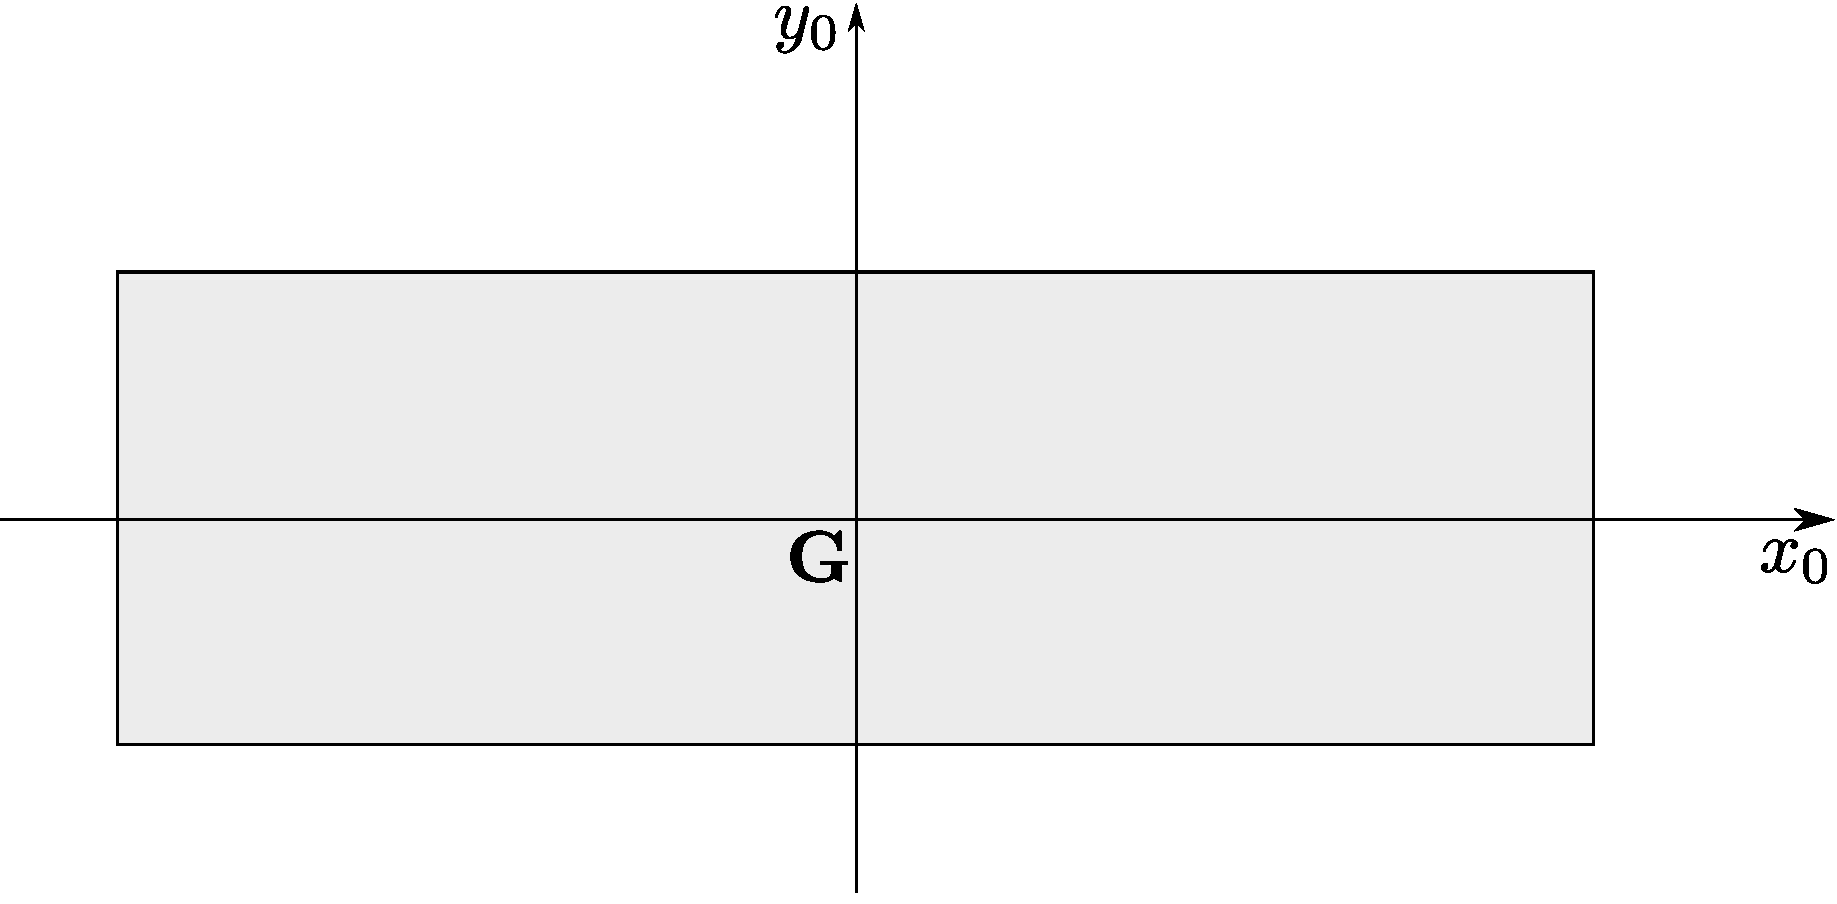
\includegraphics[width=0.37\textwidth]{Immagini/Parte_3/Figura3_2/Figura3_2.pdf}
\caption{$I_{xy_{0}} = 0 \quad \forall\,x\,\parallelsum\,x_0$   ;   $I_{x_{0}y} = 0 \quad \forall\,y\,\parallelsum\,y_0$}
\label{figura3-2}
\end{figure}
%--------------------------------------------------------------------------------------------------------------------------------------------------------------
\renewcommand{\thefigure}{3~-~3}
\begin{figure}[h]
\centering
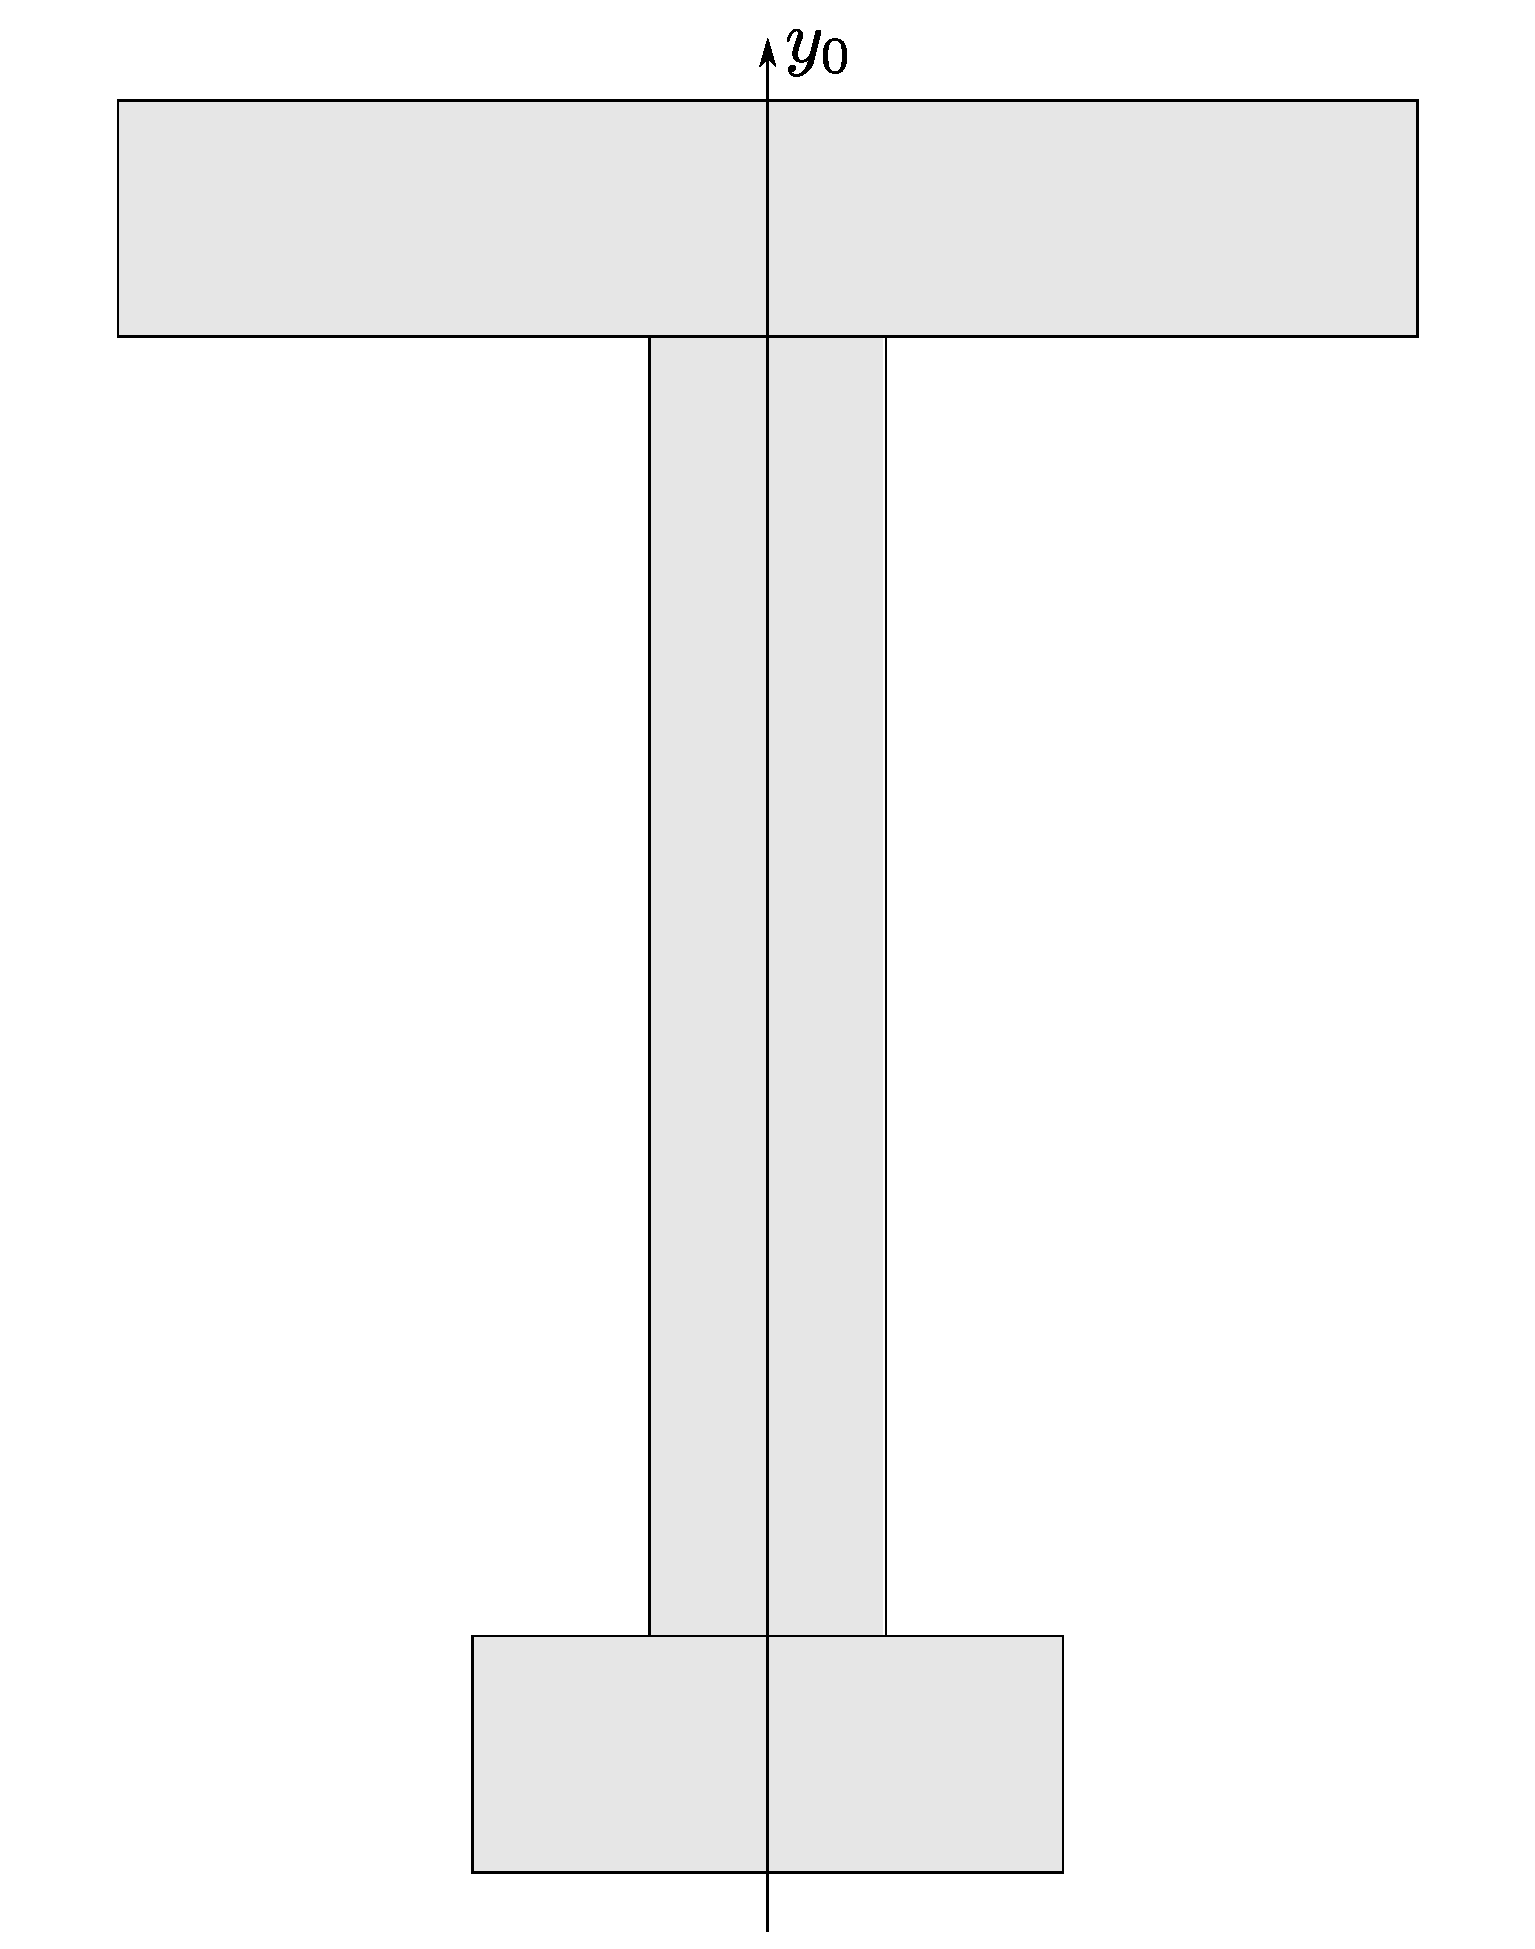
\includegraphics[width=0.34\textwidth]{Immagini/Parte_3/Figura3_3/Figura3_3.pdf}
\caption{$I_{xy_{0}} = 0 \quad \forall\,x\,\bot\,x_0$}
\label{figura3-3}
\end{figure}
%--------------------------------------------------------------------------------------------------------------------------------------------------------------
\renewcommand{\thefigure}{3~-~4}
\begin{figure}[h!]
\centering
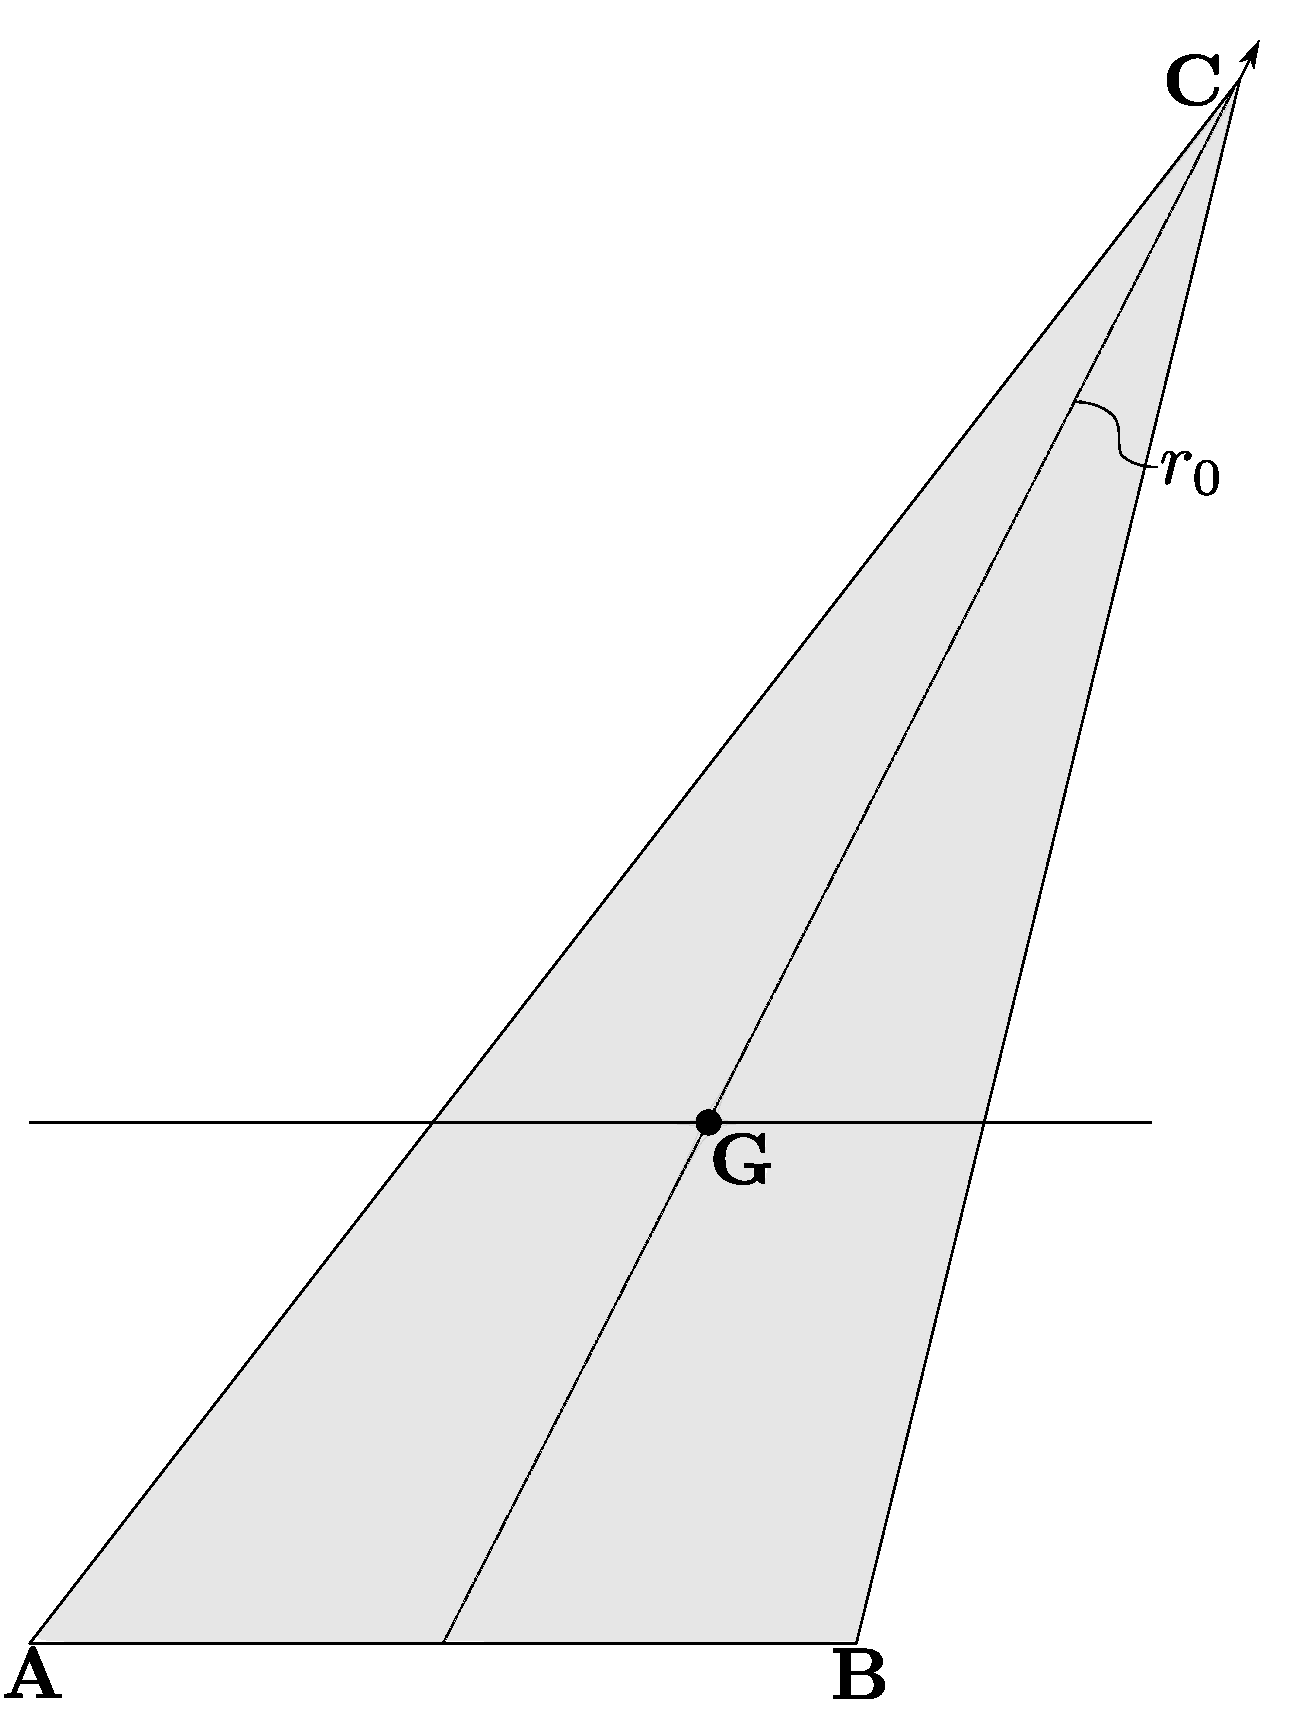
\includegraphics[width=0.34\textwidth]{Immagini/Parte_3/Figura3_4/Figura3_4.pdf}
\caption{$I_{r_{0}s} = 0 \quad \forall\,x\,\parallelsum\,AB$}
\label{figura3-4}
\end{figure}
%--------------------------------------------------------------------------------------------------------------------------------------------------------------
%--------------------------------------------------------------------------------------------------------------------------------------------------------------

\noindent Le figure~\ref{figura3-2},~\ref{figura3-3} e~\ref{figura3-4} illustrano la suddetta proposizione.
%--------------------------------------------------------------------------------------------------------------------------------------------------------------

\noindent Semplicemente osservando la~\eqref{equazione3-1} ci si rende conto, infine, della validità delle seguenti proposizioni
%--------------------------------------------------------------------------------------------------------------------------------------------------------------
\begin{equation*}
\boxed{\textup{\small Se si scambia verso ad uno dei due assi del riferimento, il momento centrifugo cambia segno}}
\end{equation*}
\begin{equation*}
\boxed{\textup{Se si cambia verso ad entrambi il momento centrifugo resta invariato}}
\end{equation*}
%--------------------------------------------------------------------------------------------------------------------------------------------------------------
In simboli
%--------------------------------------------------------------------------------------------------------------------------------------------------------------
\begin{align}
I_{(-r)s}    &= -I_{rs} \tag{3.3a} \label{equazione3-3a} \\ 
I_{r(-s)}    &= -I_{rs} \tag{3.3b} \label{equazione3-3b}\\ 
I_{(-r)(-s)} &= I_{rs} \tag{3.3c} \label{equazione3-3c}
\end{align}
%--------------------------------------------------------------------------------------------------------------------------------------------------------------
\section{Teorema del trasporto del momento centrifugo}
%--------------------------------------------------------------------------------------------------------------------------------------------------------------
\renewcommand{\thefigure}{3~-~5}
\begin{figure}[ht]
\centering
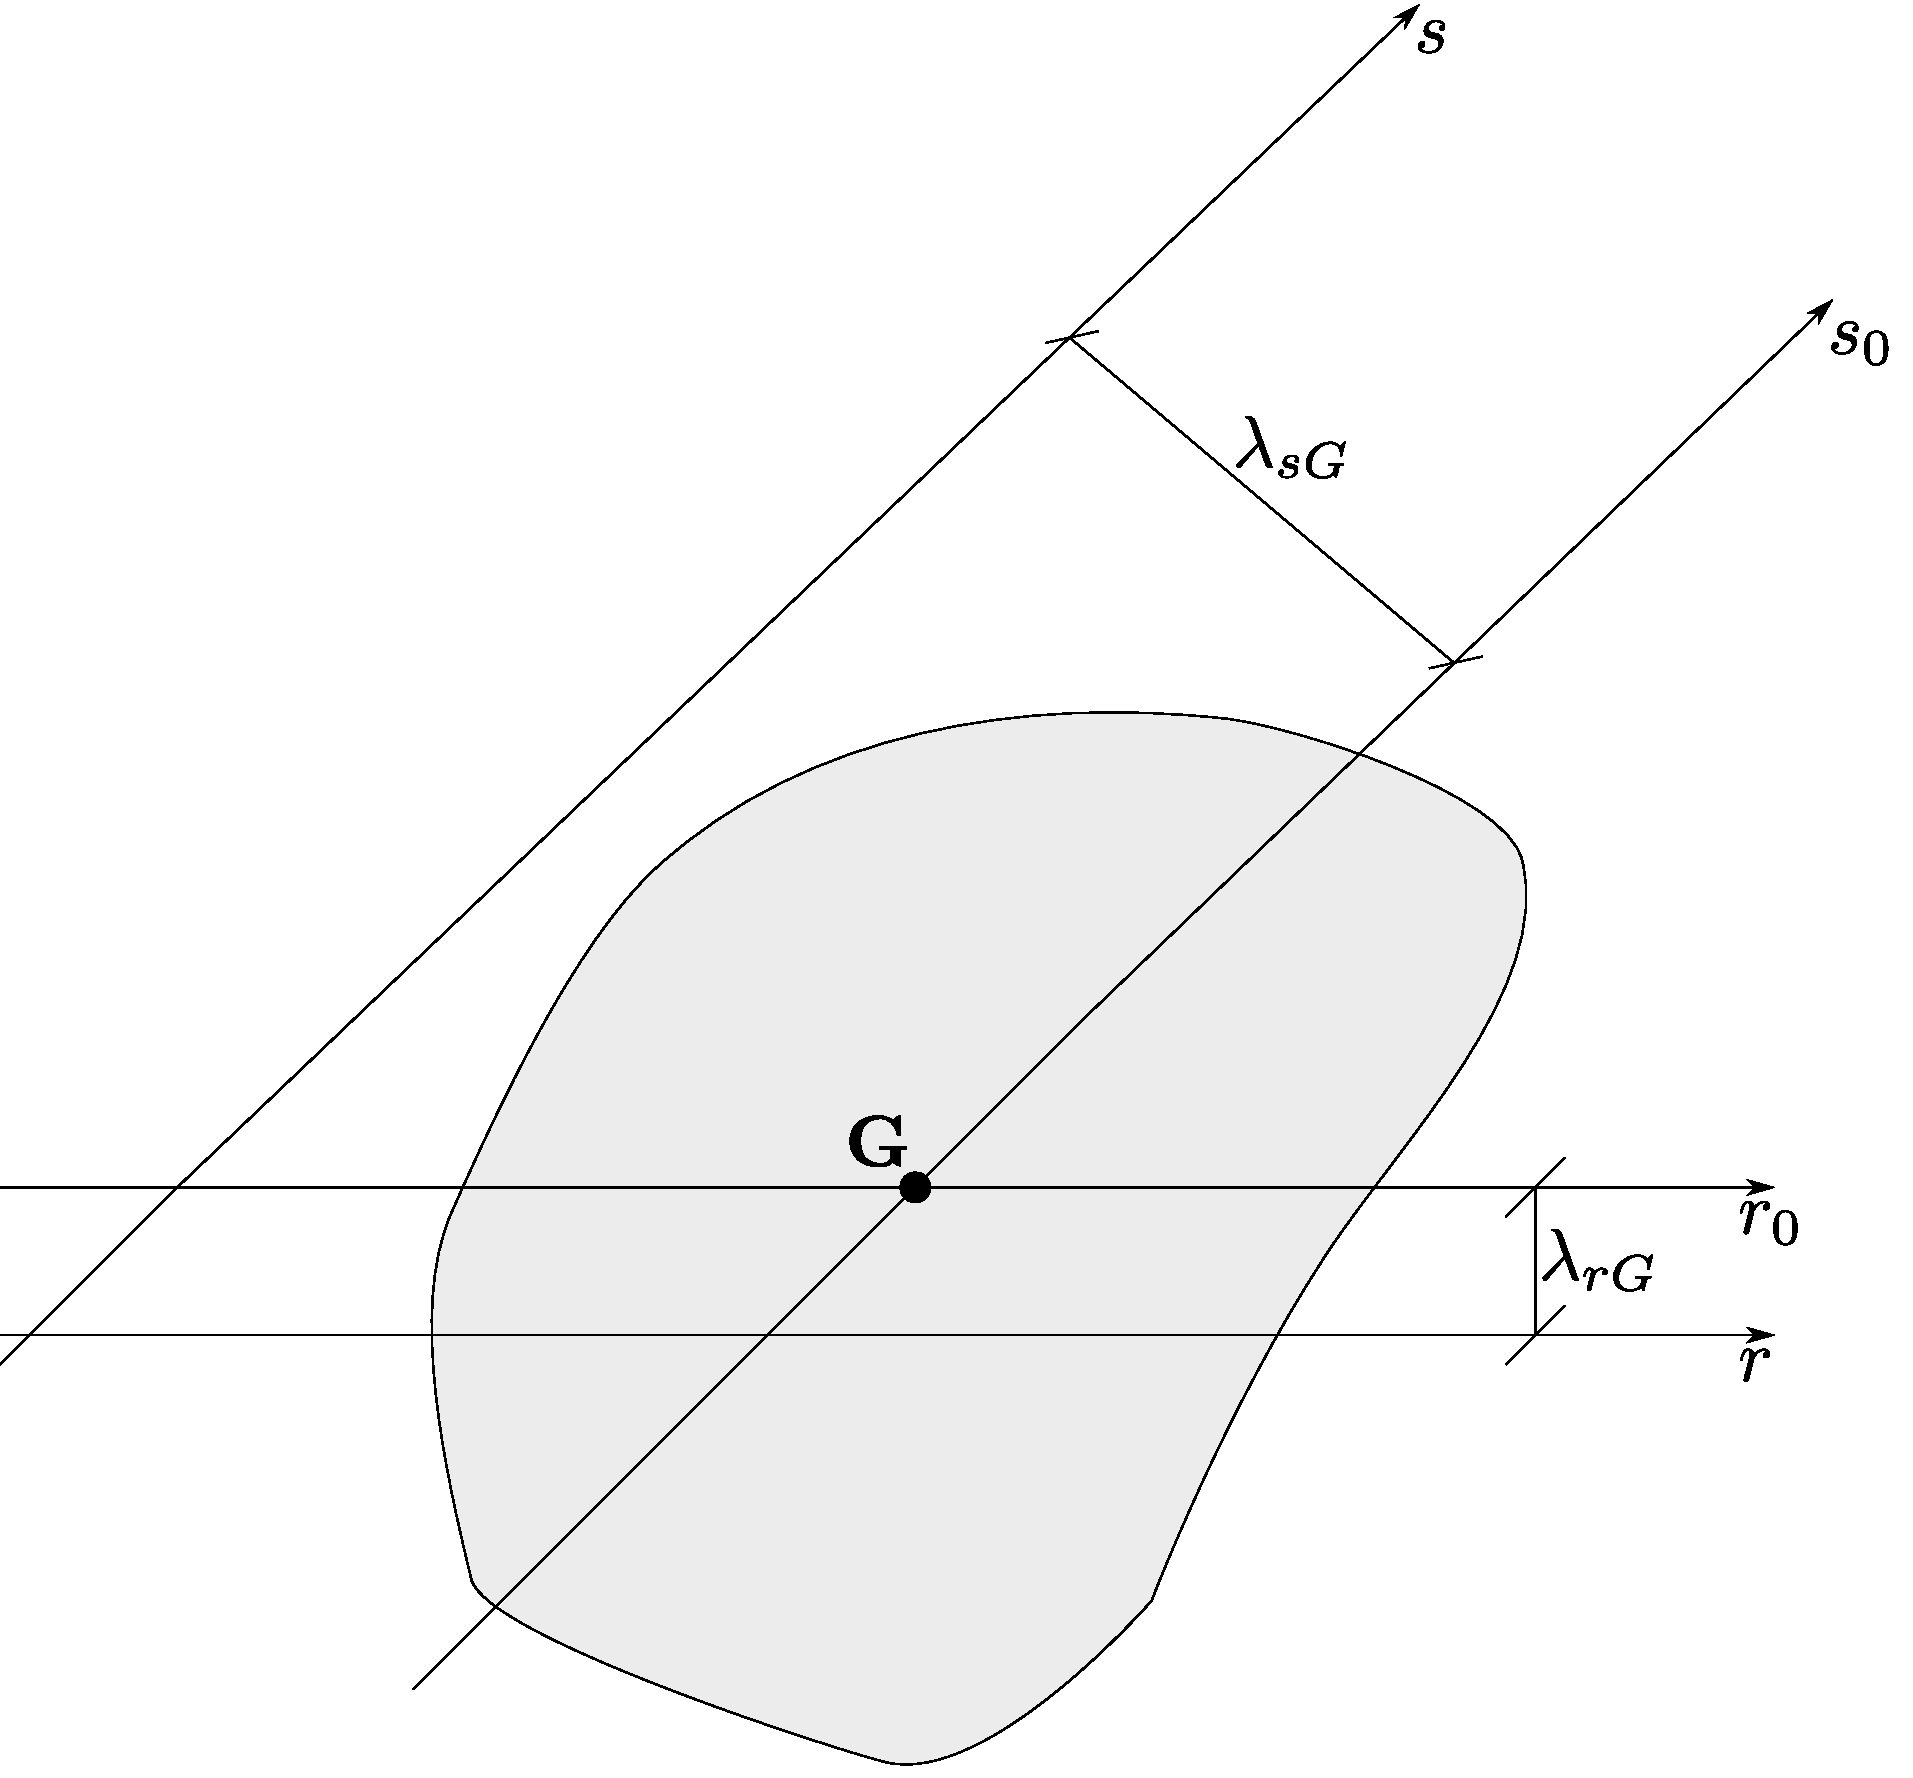
\includegraphics[width=0.73\textwidth]{Immagini/Parte_3/Figura3_5/Figura3_5.pdf}
\caption{}
\label{figura3-5}
\end{figure}
%--------------------------------------------------------------------------------------------------------------------------------------------------------------
\noindent Con riferimento alla figura~\ref{figura3-5}, si potrebbe dimostrare che 
%-------------------------------------------------------------------------------------------------------------------------------------------------------------
\begin{equation} \label{equazione3-4}
\boxed{I_{rs}=I_{r_{0}s_{0}}+A\lambda_{rG}\lambda_{sG}} \tag{3.4}
\end{equation}
%------------------------------------------------------------------------------------------------------------------------------------------------------------
Il termine $A\lambda_{rG}\lambda_{sG}$ è detto termine di trasporto; in esso $\lambda_{rG}$ e $\lambda_{sG}$ sono le distanze (con segno) del baricentro delle rette $r$ ed $s$; quindi $I_{rs}$ può essere maggiore o minore di zero. 
%--------------------------------------------------------------------------------------------------------------------------------------------------------------

\noindent Alla base della~\eqref{equazione3-4} è facile convincersi della seguente proposizione
%--------------------------------------------------------------------------------------------------------------------------------------------------------------
\begin{equation*}
\boxed{\textup{Se una retta passa per}\,\mathbf{G}\,\textup{e l'altra trasla, il momento centrifugo non varia}}
\end{equation*}
%--------------------------------------------------------------------------------------------------------------------------------------------------------------
Con riferimento alla~\ref{figura3-5}, la suddetta proposizione si traduce nei termini seguenti 
%--------------------------------------------------------------------------------------------------------------------------------------------------------------
\begin{align*}
I_{r_{0}s} &= I_{r_{0}s_{0}}, \quad \forall\,s\,\parallelsum\,s_{0} \\
I_{rs_{0}} &= I_{r_{0}s_{0}}, \quad \forall\,r\,\parallelsum\,r_{0}
\end{align*}
%--------------------------------------------------------------------------------------------------------------------------------------------------------------
Rispetto agli assi cartesiano il teorema del trasporto del momento centrifugo assume, ovviamente, la forma 
%-------------------------------------------------------------------------------------------------------------------------------------------------------------
\begin{equation} \label{equazione3-5}
\boxed{I_{xy}=I_{x_{0}y_{0}}+A\lambda_{x_{G}}\lambda_{y_{G}}} \tag{3.5}
\end{equation}
%------------------------------------------------------------------------------------------------------------------------------------------------------------
\section{Momenti centrifughi di un triangolo rettangolo}
%--------------------------------------------------------------------------------------------------------------------------------------------------------------
\renewcommand{\thefigure}{3~-~6}
\begin{figure}[ht]
\centering
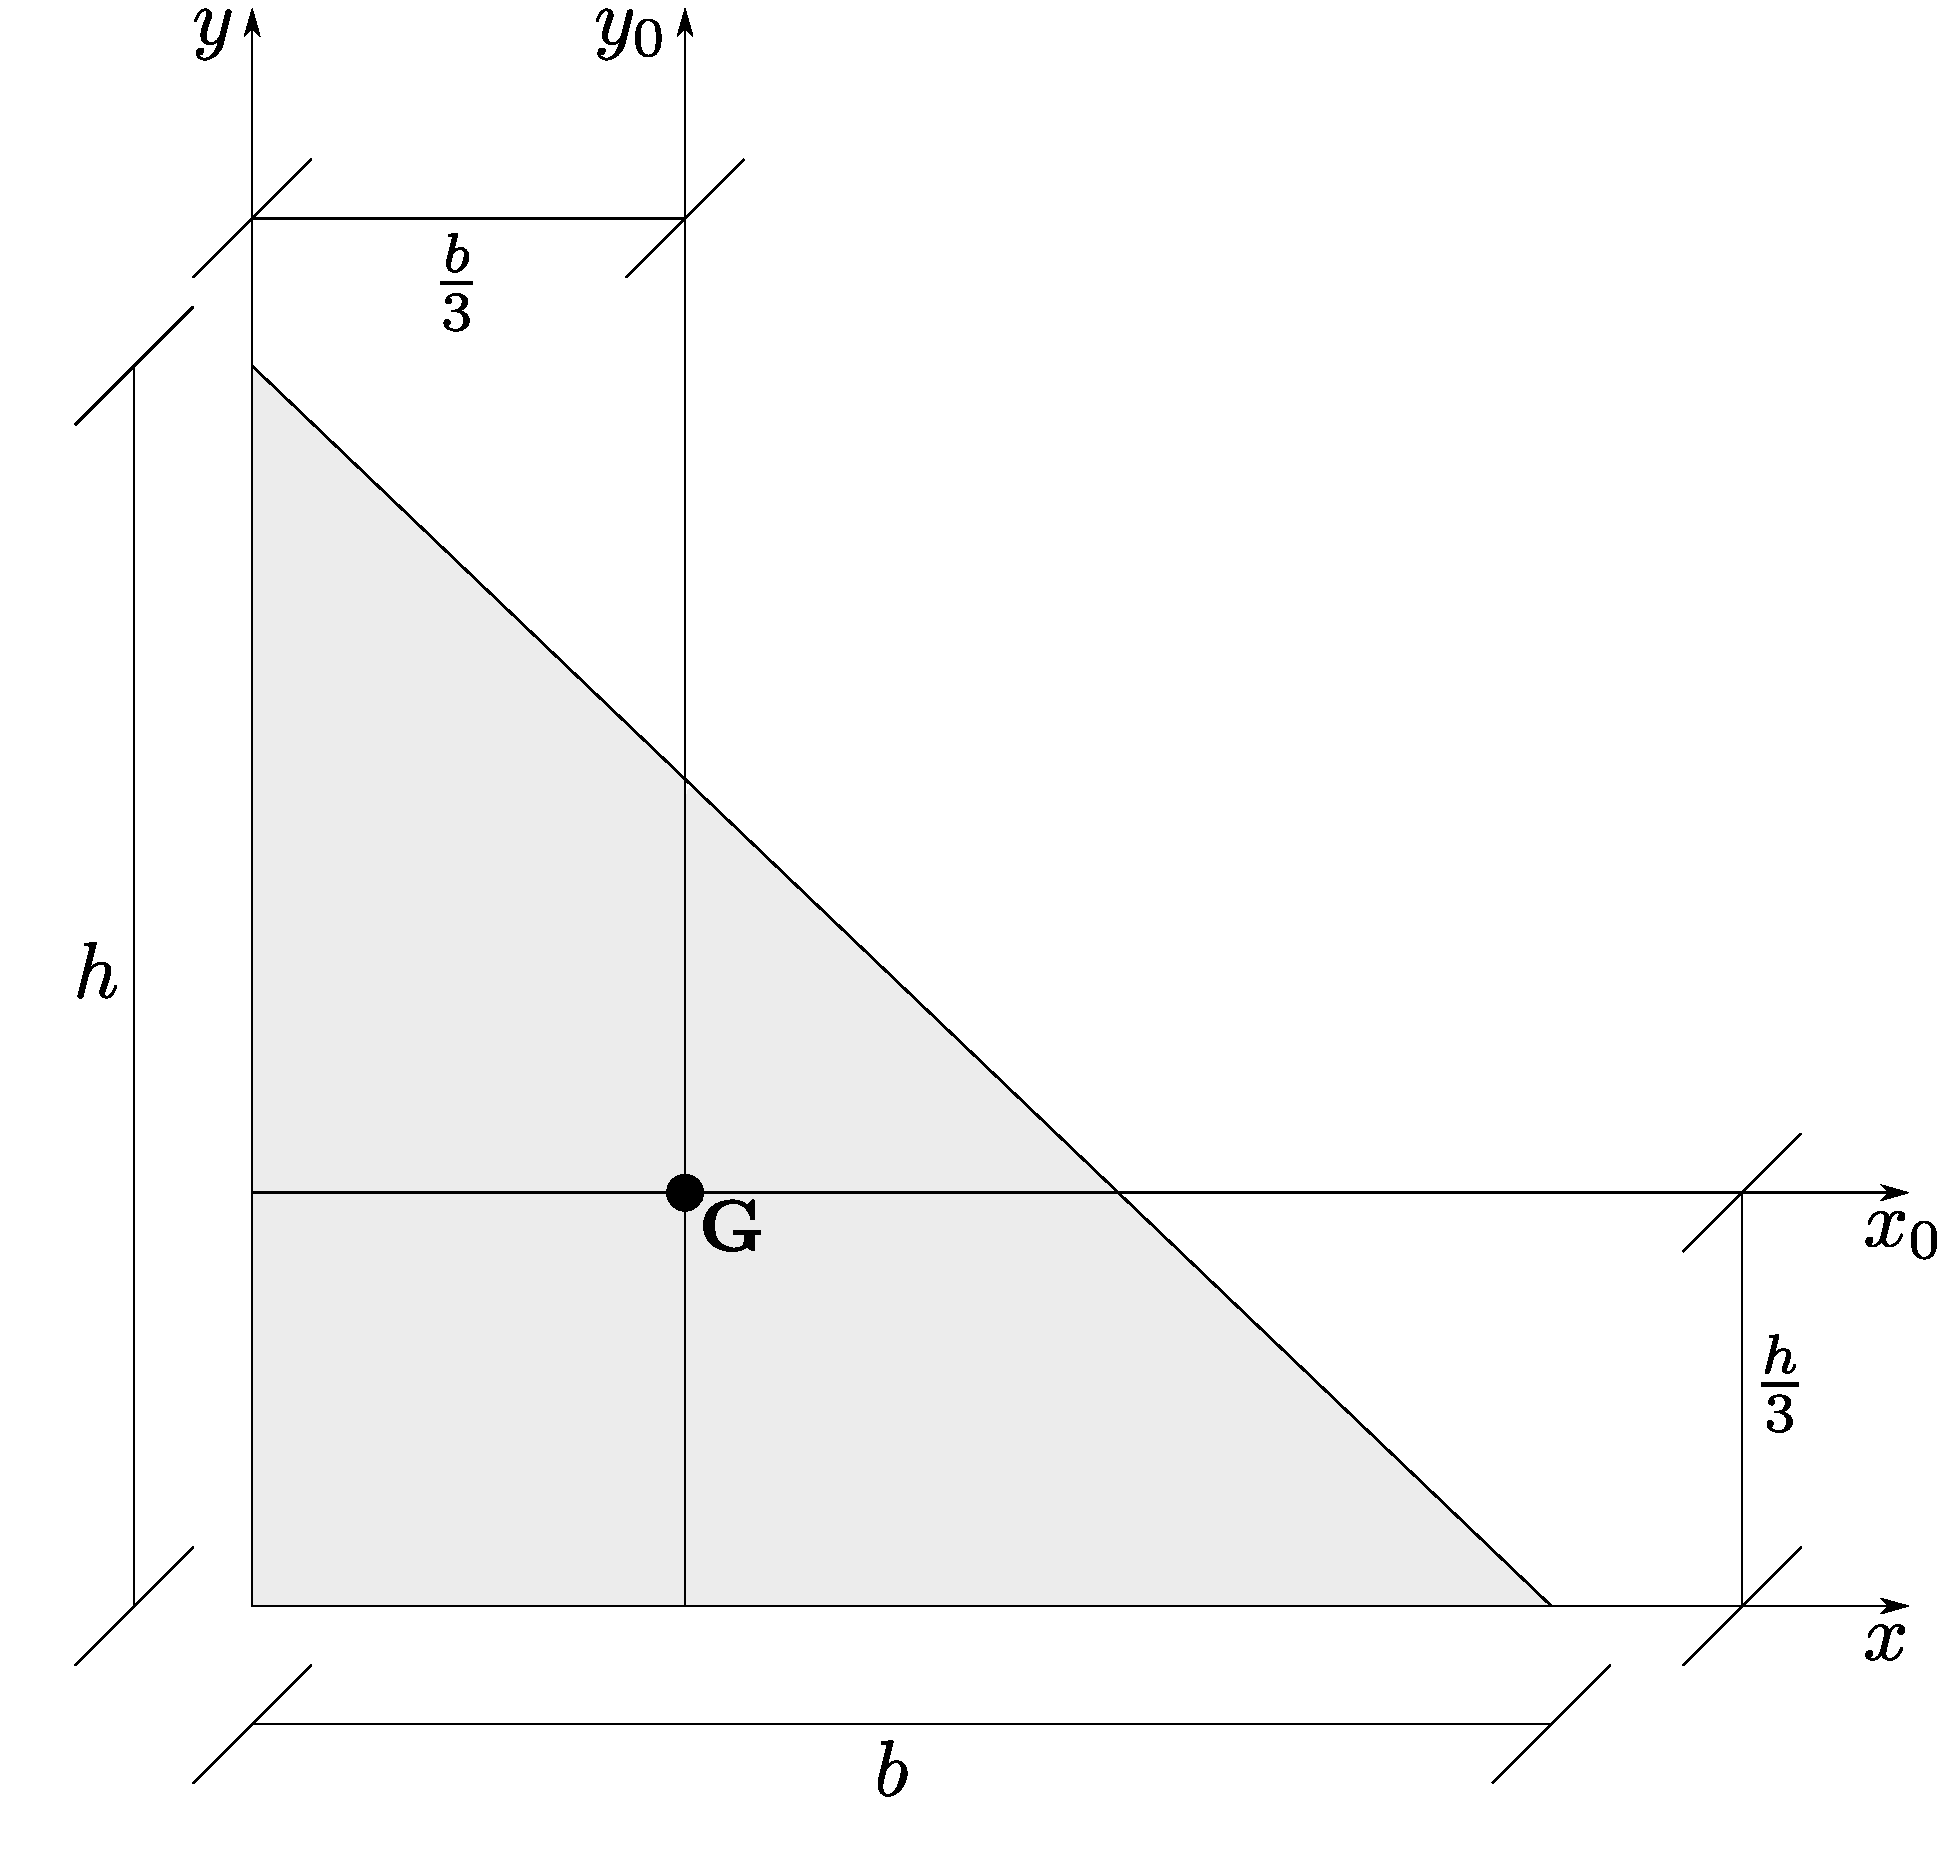
\includegraphics[width=0.62\textwidth]{Immagini/Parte_3/Figura3_6/Figura3_6.pdf}
\caption{}
\label{figura3-6}
\end{figure}
%--------------------------------------------------------------------------------------------------------------------------------------------------------------
\noindent Con riferimento alla figura~\ref{figura3-6}, ci proponiamo di calcolare prima $I_{xy}$ e poi, utilizzando il teorema del trasporto, $I_{x_{0}y_{0}}$. Cominciamo ad osservare che il lato $AB$ ha equazione
%--------------------------------------------------------------------------------------------------------------------------------------------------------------
\begin{equation*}
y = h - \frac{h}{b}x
\end{equation*}
%--------------------------------------------------------------------------------------------------------------------------------------------------------------
Dunque
%--------------------------------------------------------------------------------------------------------------------------------------------------------------
\begin{equation*}
I_{xy} = \int\int_A xydA = \int_{0}^{b}xdx\int_{0}^{h-\frac{h}{b}x}\!\!\!\!ydy = \int_{0}^{b}x\Biggl[\frac{1}{2}y^2\Biggr]_{0}^{b-\frac{h}{b}x}\!\!\!\!\!\!\!\!\!\!\!\!dx
\end{equation*}
%--------------------------------------------------------------------------------------------------------------------------------------------------------------
Ancora
%--------------------------------------------------------------------------------------------------------------------------------------------------------------
\begin{equation*}
I_{xy} = \frac{1}{2}\int_{0}^{b}x\biggl(h-\frac{h}{b}x\biggr)^{2}dx = \frac{h^{2}}{2}\int_{0}^{b}x\biggl(1+\frac{x^{2}}{b^{2}}-\frac{2}{b}x\biggr)dx = \frac{h^{2}}{2}\Biggl[\frac{x^{2}}{2}+\frac{x^4}{4b^{2}}-\frac{2}{3}\frac{x^{3}}{b}\Biggr]_{0}^{b}
\end{equation*}
%--------------------------------------------------------------------------------------------------------------------------------------------------------------
A conti fatti
%--------------------------------------------------------------------------------------------------------------------------------------------------------------
\begin{equation} \label{equazione3-6}
I_{xy} = \frac{b^{2}h^{2}}{24} \tag{3.6}
\end{equation}
%--------------------------------------------------------------------------------------------------------------------------------------------------------------
Applicando la~\eqref{equazione3-5}
%--------------------------------------------------------------------------------------------------------------------------------------------------------------
\begin{equation*}
I_{x_{0}y_{0}} = I_{xy} - Ax_{G}y_{G} = \frac{b^{2}h^{2}}{24}-\frac{1}{2}\frac{b^2}{3}\frac{h^2}{3}
\end{equation*}
%--------------------------------------------------------------------------------------------------------------------------------------------------------------
A conti fatti
%-------------------------------------------------------------------------------------------------------------------------------------------------------------
\begin{equation} \label{equazione3-7}
\boxed{I_{x_{0}y_{0}}=-\frac{b^{2}h^{2}}{72}} \tag{3.7}
\end{equation}
%--------------------------------------------------------------------------------------------------------------------------------------------------------------
\renewcommand{\thefigure}{3~-~7}
\begin{figure}[ht]
\centering
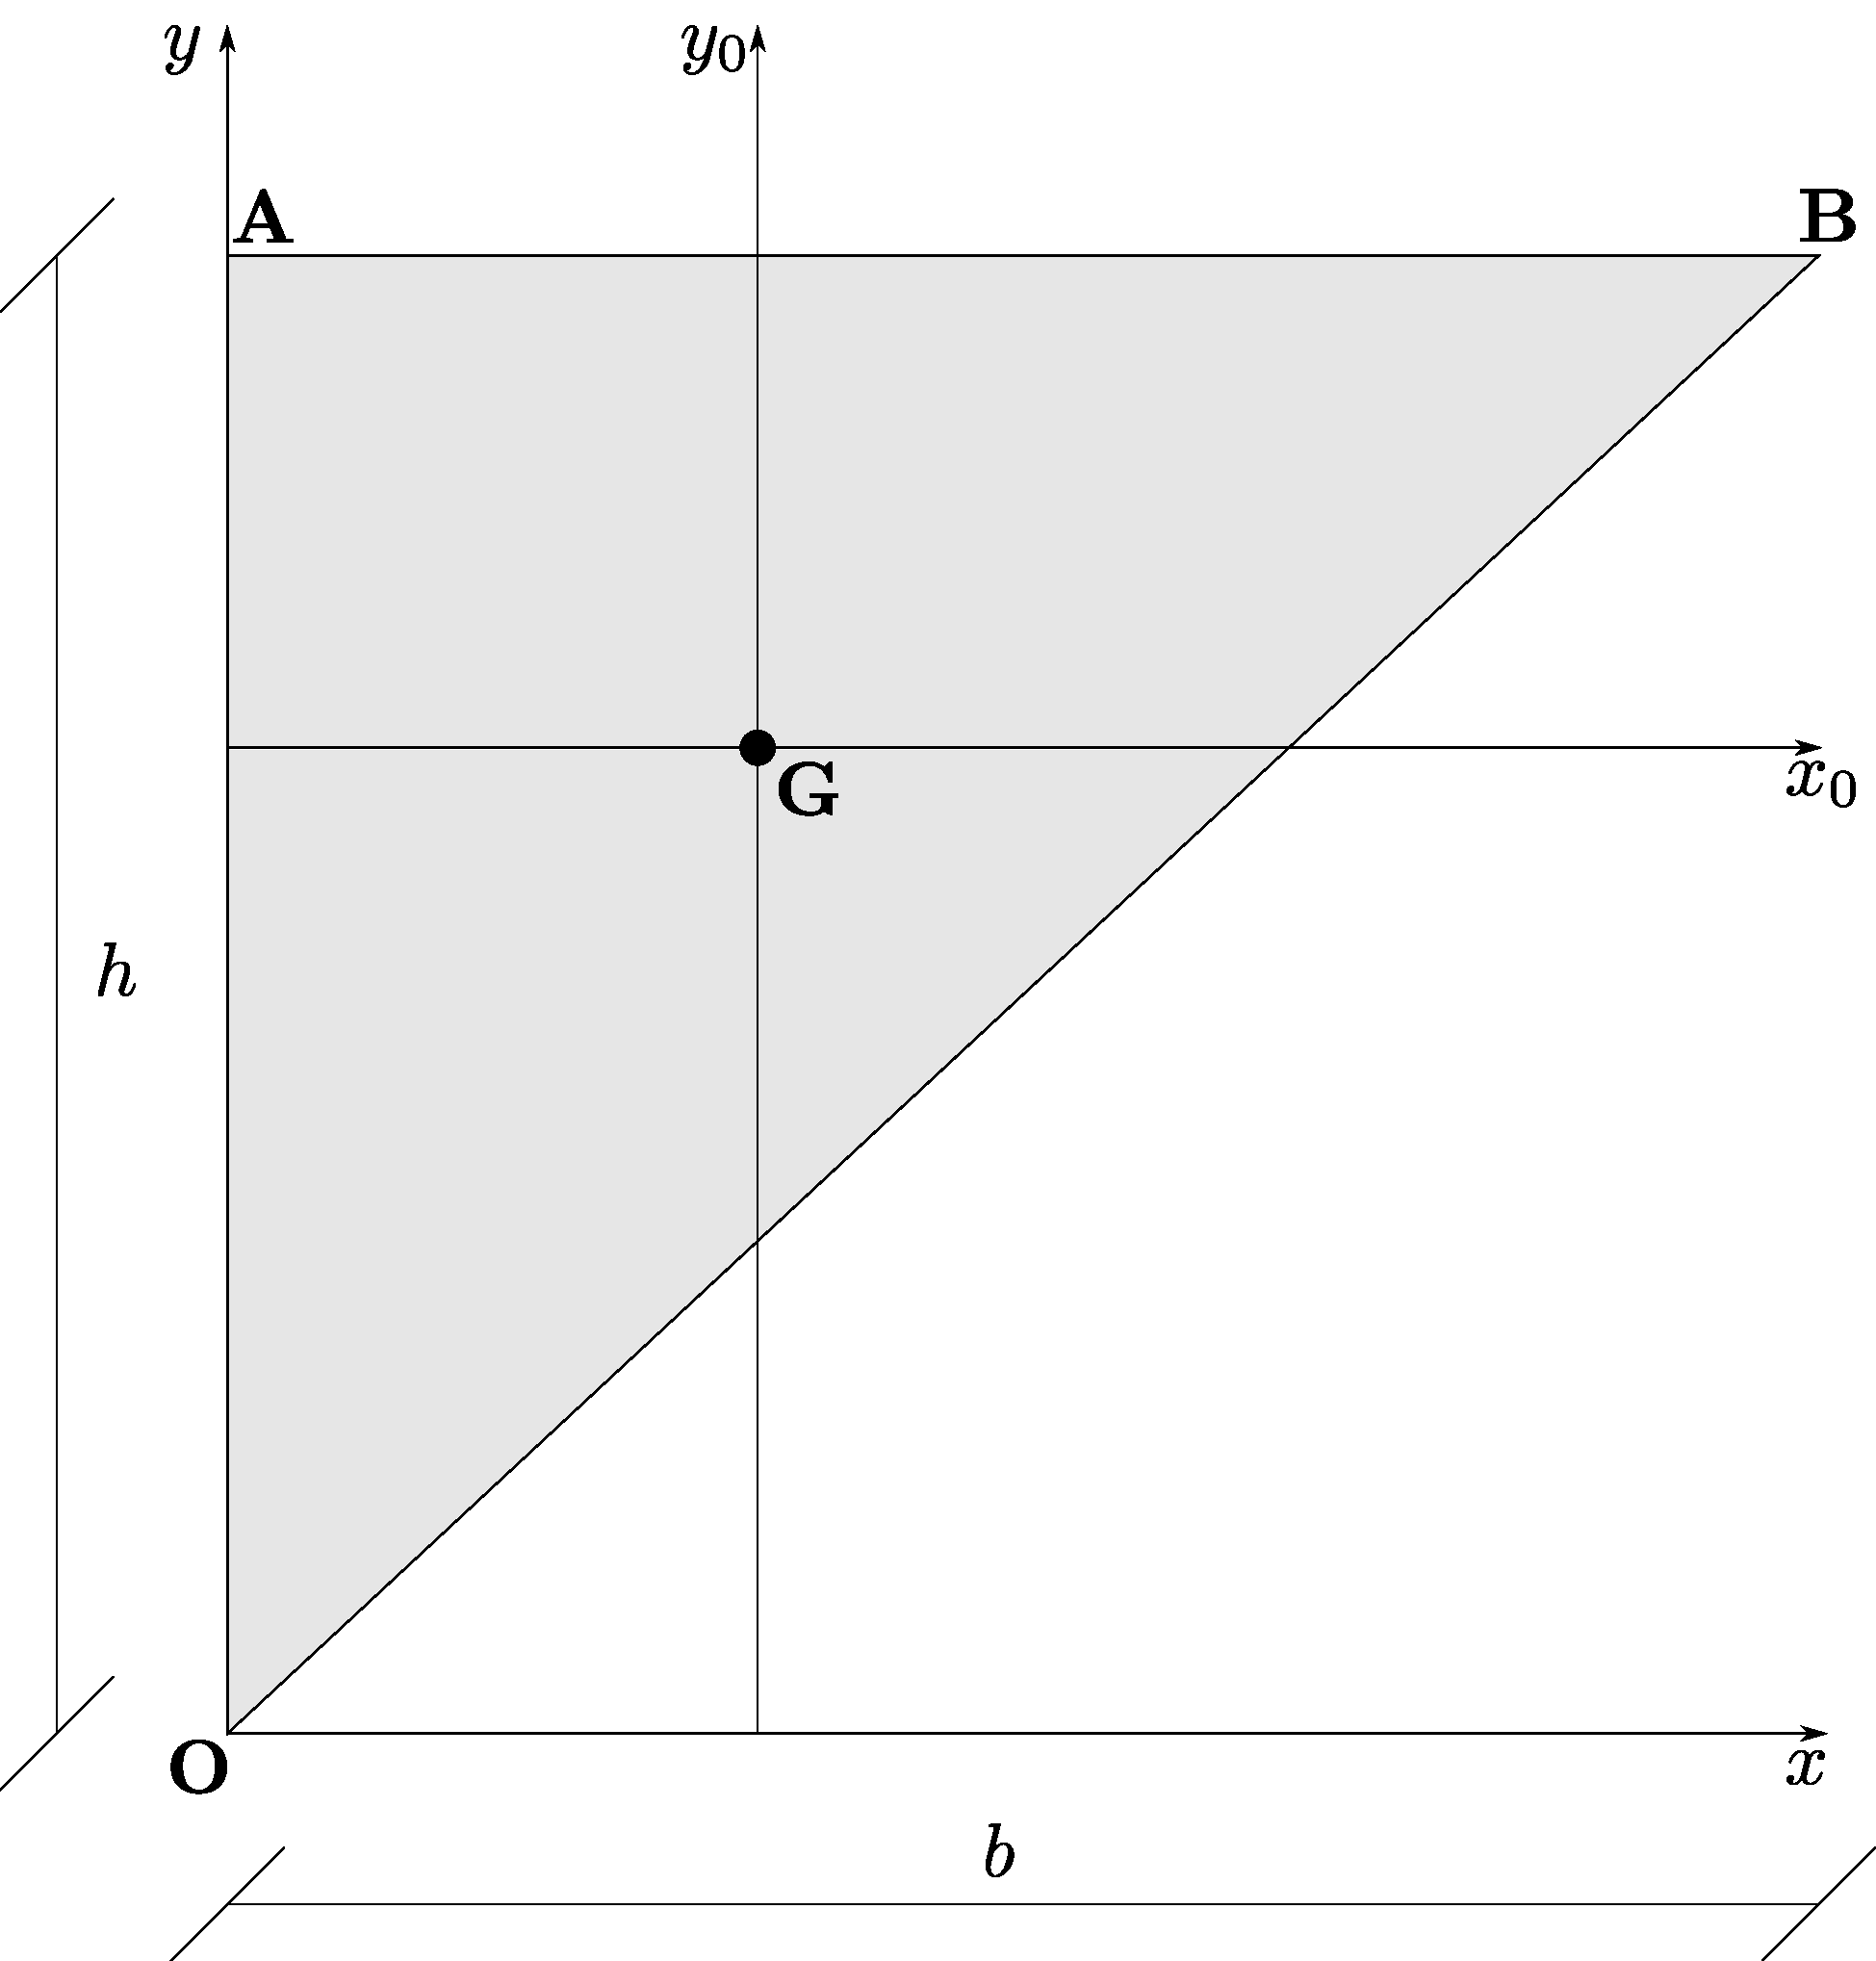
\includegraphics[width=0.45\textwidth]{Immagini/Parte_3/Figura3_7/Figura3_7.pdf}
\caption{}
\label{figura3-7}
\end{figure}
%--------------------------------------------------------------------------------------------------------------------------------------------------------------
Ed ora calcoleremo $I_{xy}$ e poi $I_{x_{0}y_{0}}$ per il triangolo rettangolo di figura~\ref{figura3-7}. Il lato $OB$ ha equazione
%--------------------------------------------------------------------------------------------------------------------------------------------------------------
\begin{equation*}
y = \frac{h}{b}x
\end{equation*}
%--------------------------------------------------------------------------------------------------------------------------------------------------------------
Dunque 
%--------------------------------------------------------------------------------------------------------------------------------------------------------------
\begin{equation*}
I_{xy} = \int\int_A xydA = \int_{0}^{b}xdx\int_{\frac{h}{b}x}^{b}ydy = \int_{0}^{b}x\biggl[\frac{1}{2}y^2\biggr]_{\frac{h}{b}x}^{b}\!\!\!\!\!\!dx = \frac{h^2}{2}\Biggl[\frac{x^2}{2}-\frac{x^4}{4b^2}\Biggr]_{0}^{b}
\end{equation*}
%--------------------------------------------------------------------------------------------------------------------------------------------------------------
A conti fatti
%--------------------------------------------------------------------------------------------------------------------------------------------------------------
\begin{equation} \label{equazione3-8}
\boxed{I_{xy}=\frac{h^{2}b^{2}}{8}}\tag{3.8}
\end{equation}
%--------------------------------------------------------------------------------------------------------------------------------------------------------------
Ed ora possiamo calcolare $I_{x_{0}y_{0}}$ applicando il teorema del trasporto
%--------------------------------------------------------------------------------------------------------------------------------------------------------------
\begin{equation*}
I_{x_{0}y_{0}} = I_{xy} - Ax_{G}y_{G} = \frac{h^{2}b^{2}}{8}-\frac{b^2}{3}\frac{h^2}{3}
\end{equation*}
%--------------------------------------------------------------------------------------------------------------------------------------------------------------
\clearpage
\section{Esercizi}
%--------------------------------------------------------------------------------------------------------------------------------------------------------------
\paragraph{Esercizi 3.1}
Calcolare $I_{xy}$ per il profilato riportato in figura.
\renewcommand{\thefigure}{3.1~-~1}
\begin{figure}[ht]
\centering
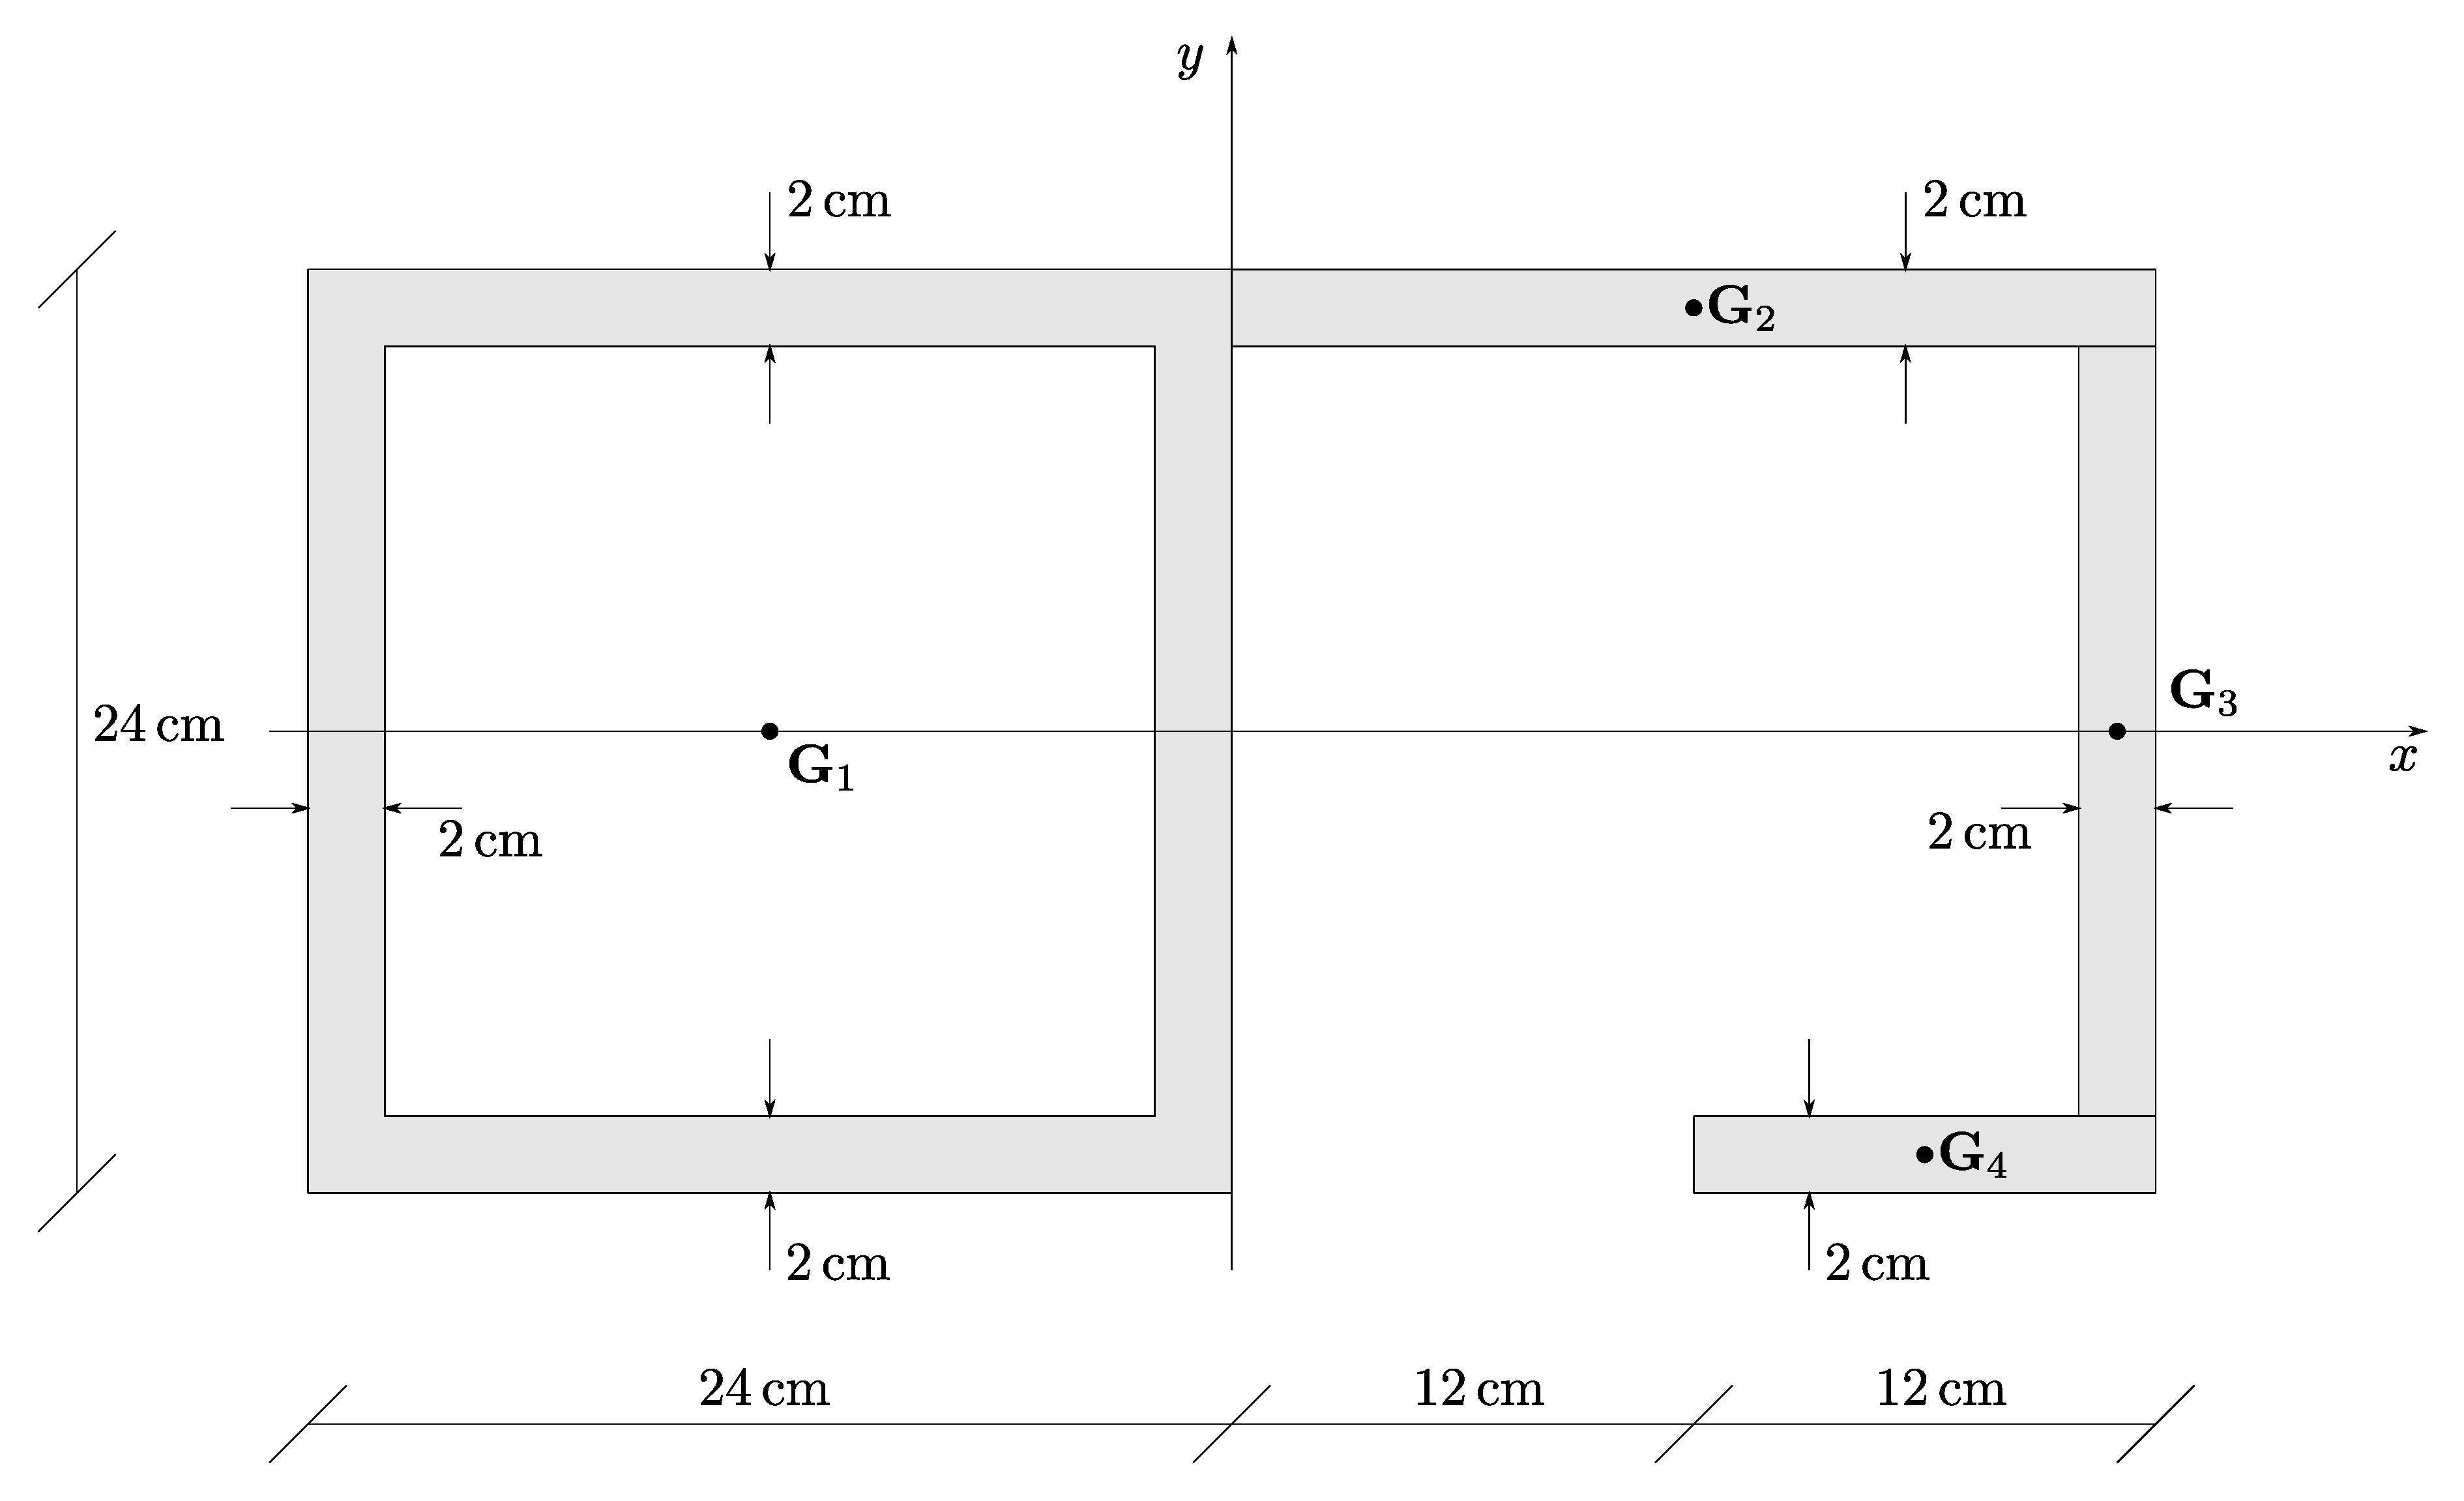
\includegraphics[width=\textwidth]{Immagini/Parte_3/Esercizio3_1/Esercizio3_1_1.pdf}
\caption{}
\label{Esercizio3_1}
\end{figure}
%--------------------------------------------------------------------------------------------------------------------------------------------------------------

\noindent Il profilato consiste di una parte \emph{chiusa}, il cui baricentro si è indicato con $\mathbf{G}_1$, e di tre rettangoli, i cui baricentri si sono indicati con $\mathbf{G}_2$, $\mathbf{G}_3$ e $\mathbf{G}_4$. 
%--------------------------------------------------------------------------------------------------------------------------------------------------------------
\begin{align*}
A_1 &= 24\times 24 -20\times 20 = 176\,\textup{cm}^2 \\ 
A_2 &= 24\times 2 = 48\,\textup{cm}^2 \\ 
A_3 &= 20\times 2 = 40\,\textup{cm}^2 \\ 
A_4 &= 12\times 2 = 24\,\textup{cm}^2
\end{align*}
%--------------------------------------------------------------------------------------------------------------------------------------------------------------
Le coordinate dei baricentri nel sistema di riferimento assunto sono
%--------------------------------------------------------------------------------------------------------------------------------------------------------------
\begin{align*}
&\mathbf{G}_1(-12, 0) \\
&\mathbf{G}_2(12, 11) \\
&\mathbf{G}_3(23, 0) \\
&\mathbf{G}_4(18, -11) 
\end{align*}
%--------------------------------------------------------------------------------------------------------------------------------------------------------------
Per ognuna delle quattro parti costituenti il nostro profilato, risulta nullo il momento centrifugo rispetto ai due assi passanti per i rispettivi baricentri e paralleli ad $x$ ed $y$; pertanto, applicando il teorema del trasporto
%-------------------------------------------------------------------------------------------------------------------------------------------------------------
\begin{align*}
I_{1xy} &= I_{1x_{0}y_{0}}+A_{1}x_{G_{1}}y_{G_{1}} = 0+0 = 0 \\ 
I_{2xy} &= I_{2x_{0}y_{0}}+A_{2}x_{G_{2}}y_{G_{2}} = 0+48\times 12\times 11 = 6336\,\textup{cm}^4 \\ 
I_{3xy} &= I_{3x_{0}y_{0}}+A_{3}x_{G_{3}}y_{G_{3}} = 0+0 = 0 \\ 
I_{4xy} &= I_{4x_{0}y_{0}}+A_{4}x_{G_{4}}y_{G_{4}} = 0+24\times 18\times (-11) = -4752\,\textup{cm}^4
\end{align*}
%--------------------------------------------------------------------------------------------------------------------------------------------------------------
In definitiva, essendo il momento centrifugo una grandezza additiva come l'area, il momento statico ed il momento di inerzia
%--------------------------------------------------------------------------------------------------------------------------------------------------------------
\begin{equation*}
I_{xy} = 6336-4752 = 1584\,\textup{cm}^4
\end{equation*}
%--------------------------------------------------------------------------------------------------------------------------------------------------------------
\clearpage
\paragraph{Esercizio 3.2}
Calcolare il momento centrifugo $I_{xy}$ per il settore di corona circolare di spessore molto sottile già considerato nell'Esercizio $1.7$.
%--------------------------------------------------------------------------------------------------------------------------------------------------------------
\newline 

\noindent Al solito 
%--------------------------------------------------------------------------------------------------------------------------------------------------------------
\begin{align*}
I_{xy} &= \int\int_A xydA = \int\int_A (r\cos\varphi)(r\sin\varphi)rdrd\varphi = \int_{R_i}^{R_e}r^{3}dr\int_{\alpha}^{\beta} \sin\varphi\cos\varphi d\varphi \\
          &= \frac{R_{e}^{4}-R_{i}^{4}}{4}\frac{1}{2}\bigl[\sin^{2}\varphi\bigr]_{\alpha}^{\beta}
\end{align*}
%--------------------------------------------------------------------------------------------------------------------------------------------------------------
In definitiva si ottiene 
%--------------------------------------------------------------------------------------------------------------------------------------------------------------
\begin{equation*}
\boxed{\textup{\textsc{Formula esatta}}} \longrightarrow \boxed{I_{xy} = \frac{R_{e}^{4}-R_{i}^{4}}{8}(\sin^{2}\beta-\sin^{2}\alpha)}
\end{equation*}
%--------------------------------------------------------------------------------------------------------------------------------------------------------------
Posto
%--------------------------------------------------------------------------------------------------------------------------------------------------------------
\begin{align*}
R_e &= r_m + \frac{\delta}{2} \\
R_i  &= r_m - \frac{\delta}{2}
\end{align*}
%--------------------------------------------------------------------------------------------------------------------------------------------------------------
si trova 
%--------------------------------------------------------------------------------------------------------------------------------------------------------------
\begin{equation*}
R_{e}^{4}-R_{i}^{4} = r_{m}\delta(4r_{m}^{2}+\delta^2) = r_{m}^{2}\delta\biggl(4+\frac{\delta^2}{r_{m}^{2}}\biggr)
\end{equation*}
%--------------------------------------------------------------------------------------------------------------------------------------------------------------
Trascurando il termine $\frac{\delta^2}{r_{m}^{2}}$ rispetto a $4$
%--------------------------------------------------------------------------------------------------------------------------------------------------------------
\begin{equation*}
R_{e}^{4}-R_{i}^{4} \equiv 4r_{m}^{3}\delta 
\end{equation*}
%--------------------------------------------------------------------------------------------------------------------------------------------------------------
e quindi
%--------------------------------------------------------------------------------------------------------------------------------------------------------------
\begin{equation*}
\boxed{\textup{\textsc{Formula approssimata}}} \longrightarrow \boxed{I_{xy} = \frac{1}{2}r_{m}^{3}\delta(\sin^{2}\beta-\sin^{2}\alpha)}
\end{equation*}
%--------------------------------------------------------------------------------------------------------------------------------------------------------------
L'errore insito nella formula approssimata, nel caso in cui $\frac{\delta}{r_{m}}=10$, è un po' minore dello $0.25\%$.
%--------------------------------------------------------------------------------------------------------------------------------------------------------------
%------------------------------------------------
\clearpage
\pagestyle{fancy}
\part{Assi principali di inerzia}
\setcounter{section}{0}
\section{Formule di trasformazione}
%--------------------------------------------------------------------------------------------------------------------------------------------------------------
\renewcommand{\thefigure}{4~-~1}
\begin{figure}[ht]
\centering
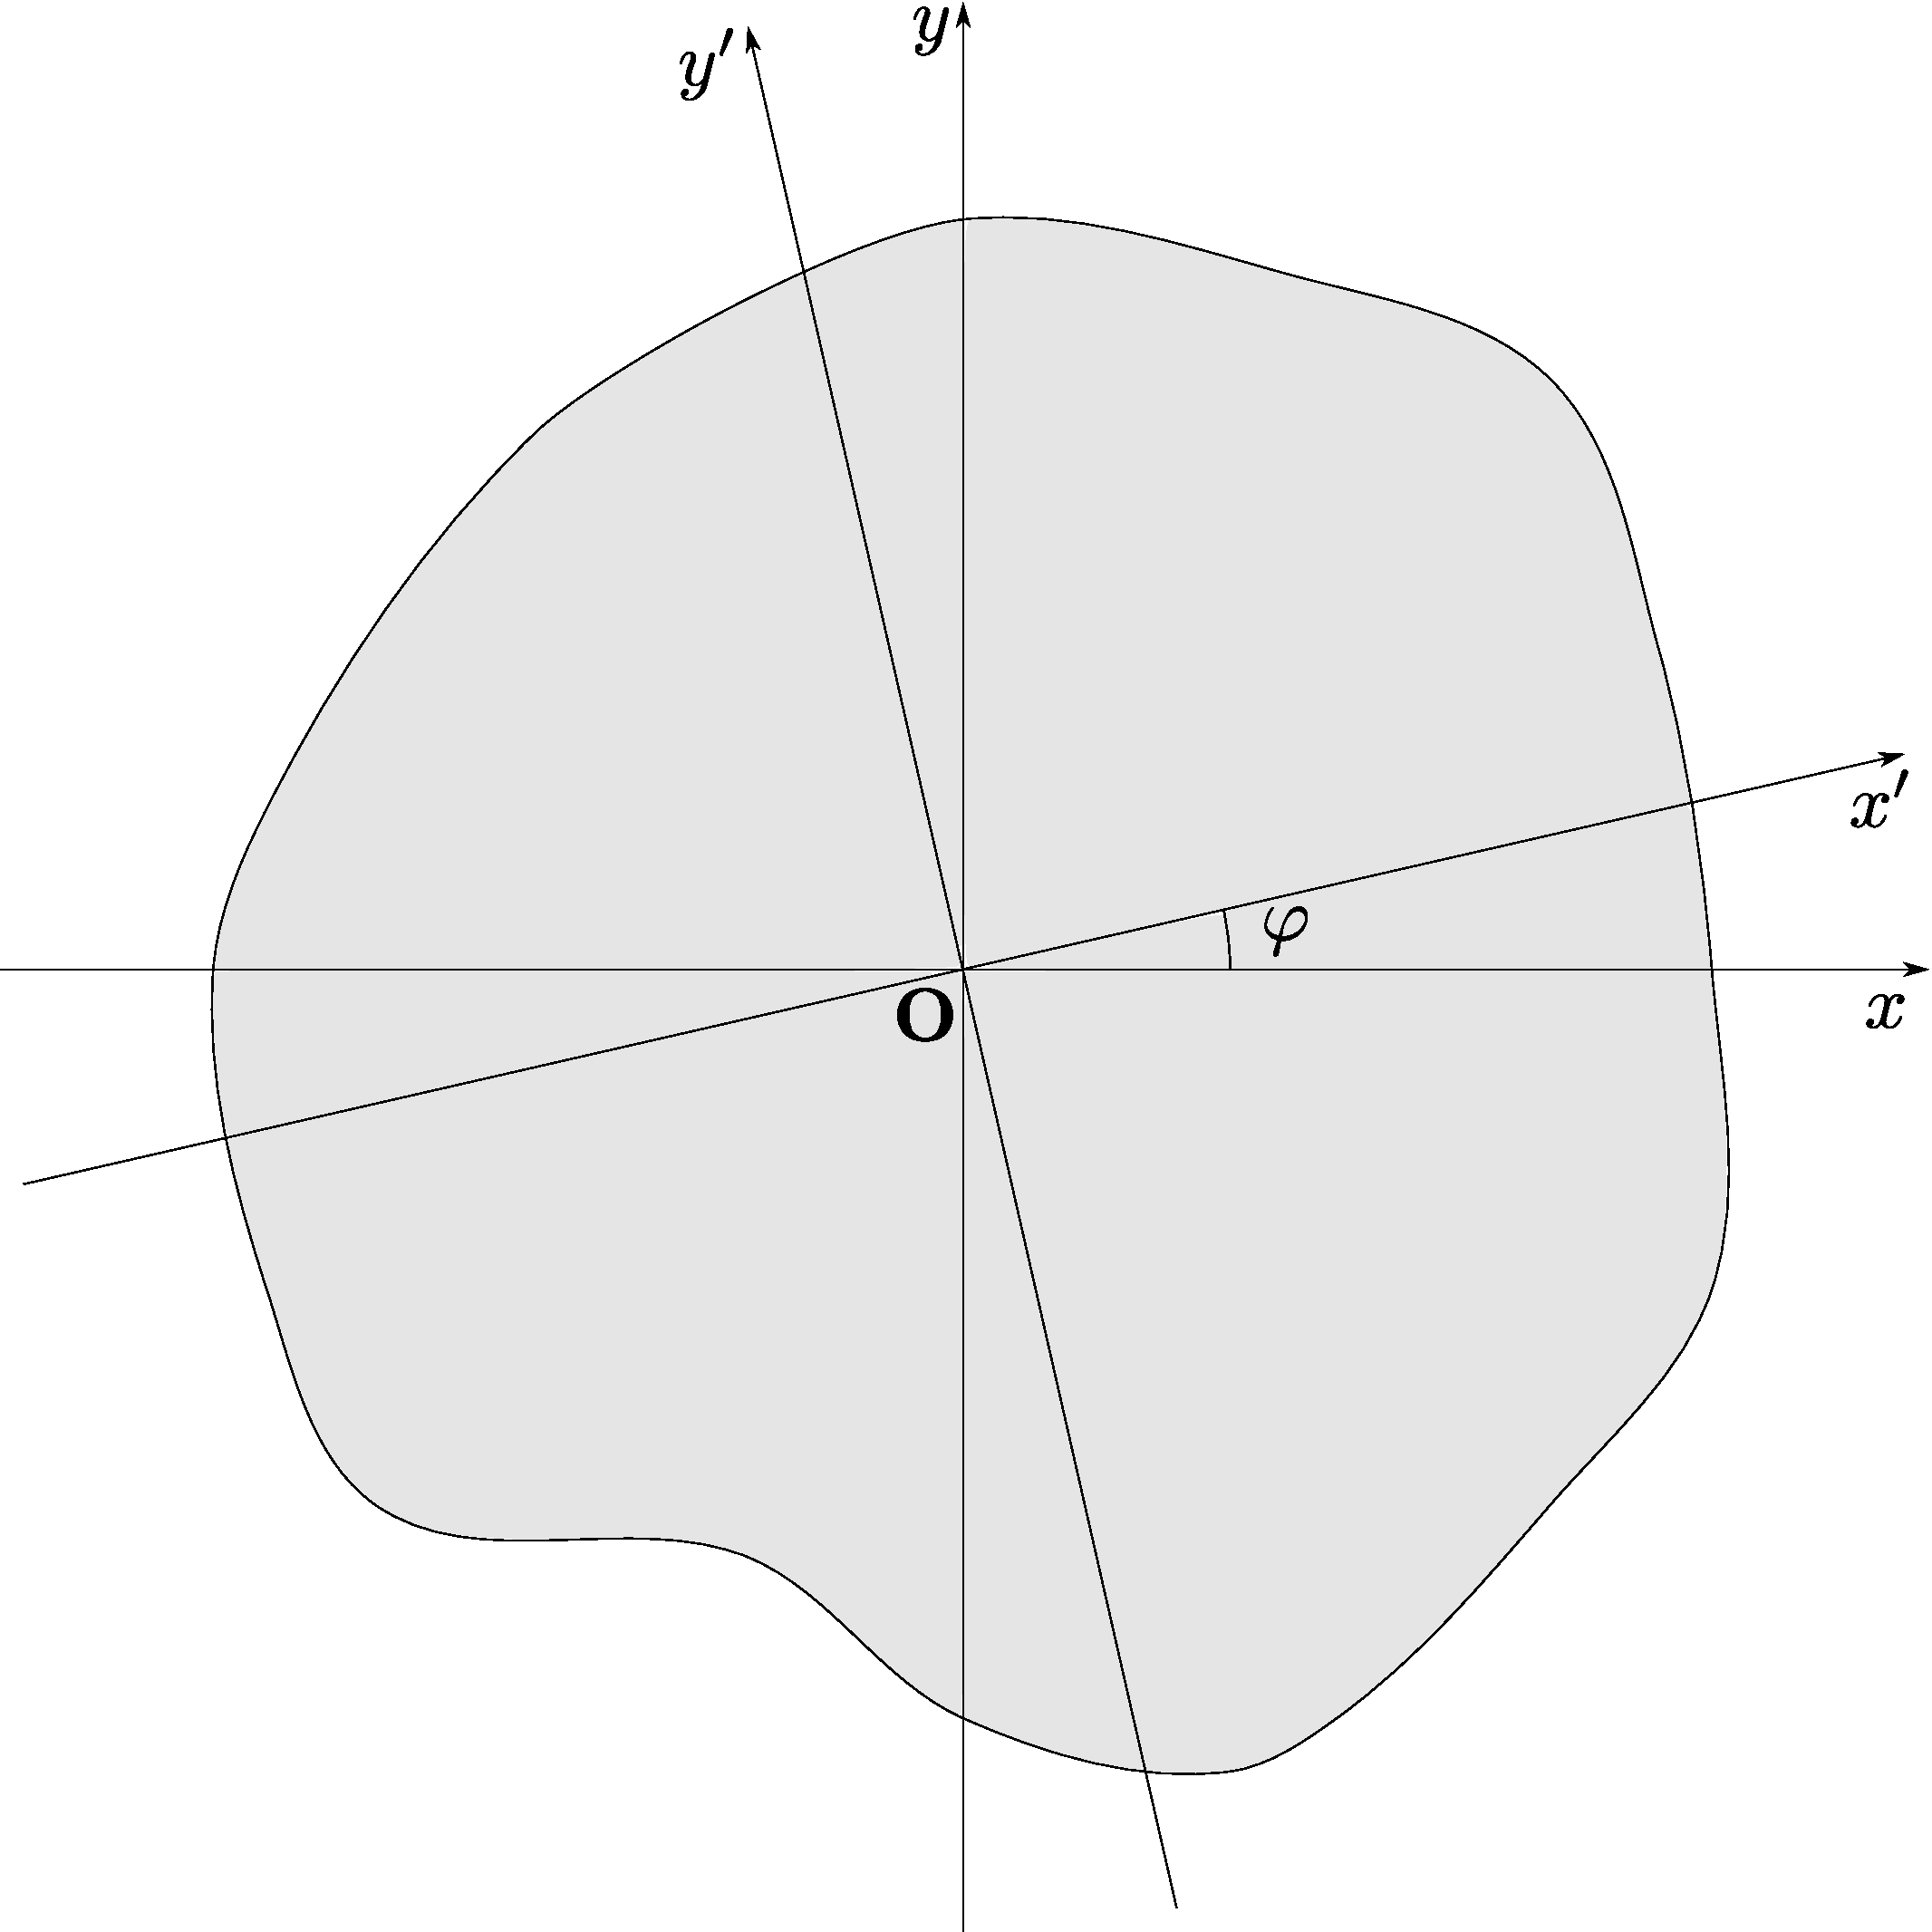
\includegraphics[width=0.65\textwidth]{Immagini/Parte_4/Figura4_1/Figura4_1.pdf}
\caption{}
\label{figura4-1}
\end{figure}
%--------------------------------------------------------------------------------------------------------------------------------------------------------------
\noindent Con riferimento alla figura~\ref{figura4-1}, ci poniamo il seguente quesito: 
%--------------------------------------------------------------------------------------------------------------------------------------------------------------
\begin{quoting}
Noti $I_x$, $I_y$ ed $I_{xy}$ è possibile ricavare $I_{x'}$, $I_{y'}$ ed $I_{x'y'}$?
\end{quoting}
%--------------------------------------------------------------------------------------------------------------------------------------------------------------
Ebbene, la risposta è affermativa, essendo valide le seguenti
%--------------------------------------------------------------------------------------------------------------------------------------------------------------
\begin{equation} \label{equazione4-1}
\boxed{\textup{\textsc{Formule di trasformazione}}} \longrightarrow
\begin{aligned}
I_{x'} &= I_{x}\cos^{2}\varphi+I_{y}\sin^{2}\varphi-I_{xy}\sin 2\varphi \\ 
I_{y'} &= I_{x}\sin^{2}\varphi+I_{y}\cos^{2}\varphi+I_{xy}\sin 2\varphi \\
I_{x'y'} &= \frac{I_{x}-I_{y}}{2}\sin 2\varphi+I_{xy}\cos 2\varphi
\end{aligned}
\tag{4.1}
\end{equation}
%--------------------------------------------------------------------------------------------------------------------------------------------------------------
Per una corretta utilizzazione delle~\eqref{equazione4-1} vale la pena sottolineare che
%--------------------------------------------------------------------------------------------------------------------------------------------------------------
\begin{enumerate}
\item i due riferimento $\mathbf{O}\,x\,y$ ed $\mathbf{O}\,x'\,y'$ devono avere in comune l'origine ed essere entrambi \textsc{ortogonali} e \textsc{levogiri};
\item $\varphi$ è l'angolo di cui $x'$ è ruotato rispetto ad $x$; esso deve essere misurato in senso antiorario, essendo ovviamente $0\le\varphi\le 2\pi$.
\end{enumerate}
%--------------------------------------------------------------------------------------------------------------------------------------------------------------
Le~\eqref{equazione4-1} si dimostrano agevolmente utilizzando le seguenti, ben note
%--------------------------------------------------------------------------------------------------------------------------------------------------------------
\begin{equation*}
\boxed{\textup{\textsc{Formule di trasformazione delle coordinate}}} \longrightarrow
\begin{aligned}
x' &= x\cos\varphi+y\sin\varphi \notag \\ 
y' &= -x\sin\varphi+y\cos\varphi \notag
\end{aligned}
\end{equation*}
%--------------------------------------------------------------------------------------------------------------------------------------------------------------
Dimostriamo, a titolo di esempio, solo la terza delle~\eqref{equazione4-1}:
%--------------------------------------------------------------------------------------------------------------------------------------------------------------
\begin{align*}
I_{x'y'} &= \int\int_A x'y'dA = \int\int_A (x\cos\varphi+y\sin\varphi)(-x\sin\varphi+y\cos\varphi)dA = \\
           &= \int\int_A (-x^{2}\sin\varphi\cos\varphi-xy\sin^{2}\varphi+xy\cos^{2}\varphi+y^{2}\sin\varphi\cos\varphi)dA
\end{align*}
%--------------------------------------------------------------------------------------------------------------------------------------------------------------
essendo $\varphi$ costante rispetto a $dA$ e tenendo presente che
%--------------------------------------------------------------------------------------------------------------------------------------------------------------
\begin{equation*}
\,\,\biggl\{\,\
\begin{aligned}
2\sin\varphi\cos\varphi &= \sin 2\varphi \\
\cos^{2}\varphi-\sin^{2}\varphi  &= \cos 2\varphi
\end{aligned}
\end{equation*}
%--------------------------------------------------------------------------------------------------------------------------------------------------------------
possiamo dunque scrivere
%--------------------------------------------------------------------------------------------------------------------------------------------------------------
\begin{align*}
I_{x'y'} &= \frac{1}{2}\sin 2\varphi\int\int_A y^{2}dA + \frac{1}{2}\sin 2\varphi\int\int_A x^{2}dA +\cos\varphi\int\int_{A}xydA= \\
           &=  I_{x}\frac{1}{2}\sin 2\varphi + I_{y}\frac{1}{2}\sin 2\varphi +I_{xy}\cos\varphi
\end{align*}
%--------------------------------------------------------------------------------------------------------------------------------------------------------------
che è quanto volevamo ottenere
%--------------------------------------------------------------------------------------------------------------------------------------------------------------
\section{Gli assi principali di inerzia}
%--------------------------------------------------------------------------------------------------------------------------------------------------------------
\renewcommand{\thefigure}{4~-~2}
\begin{figure}[ht]
\centering
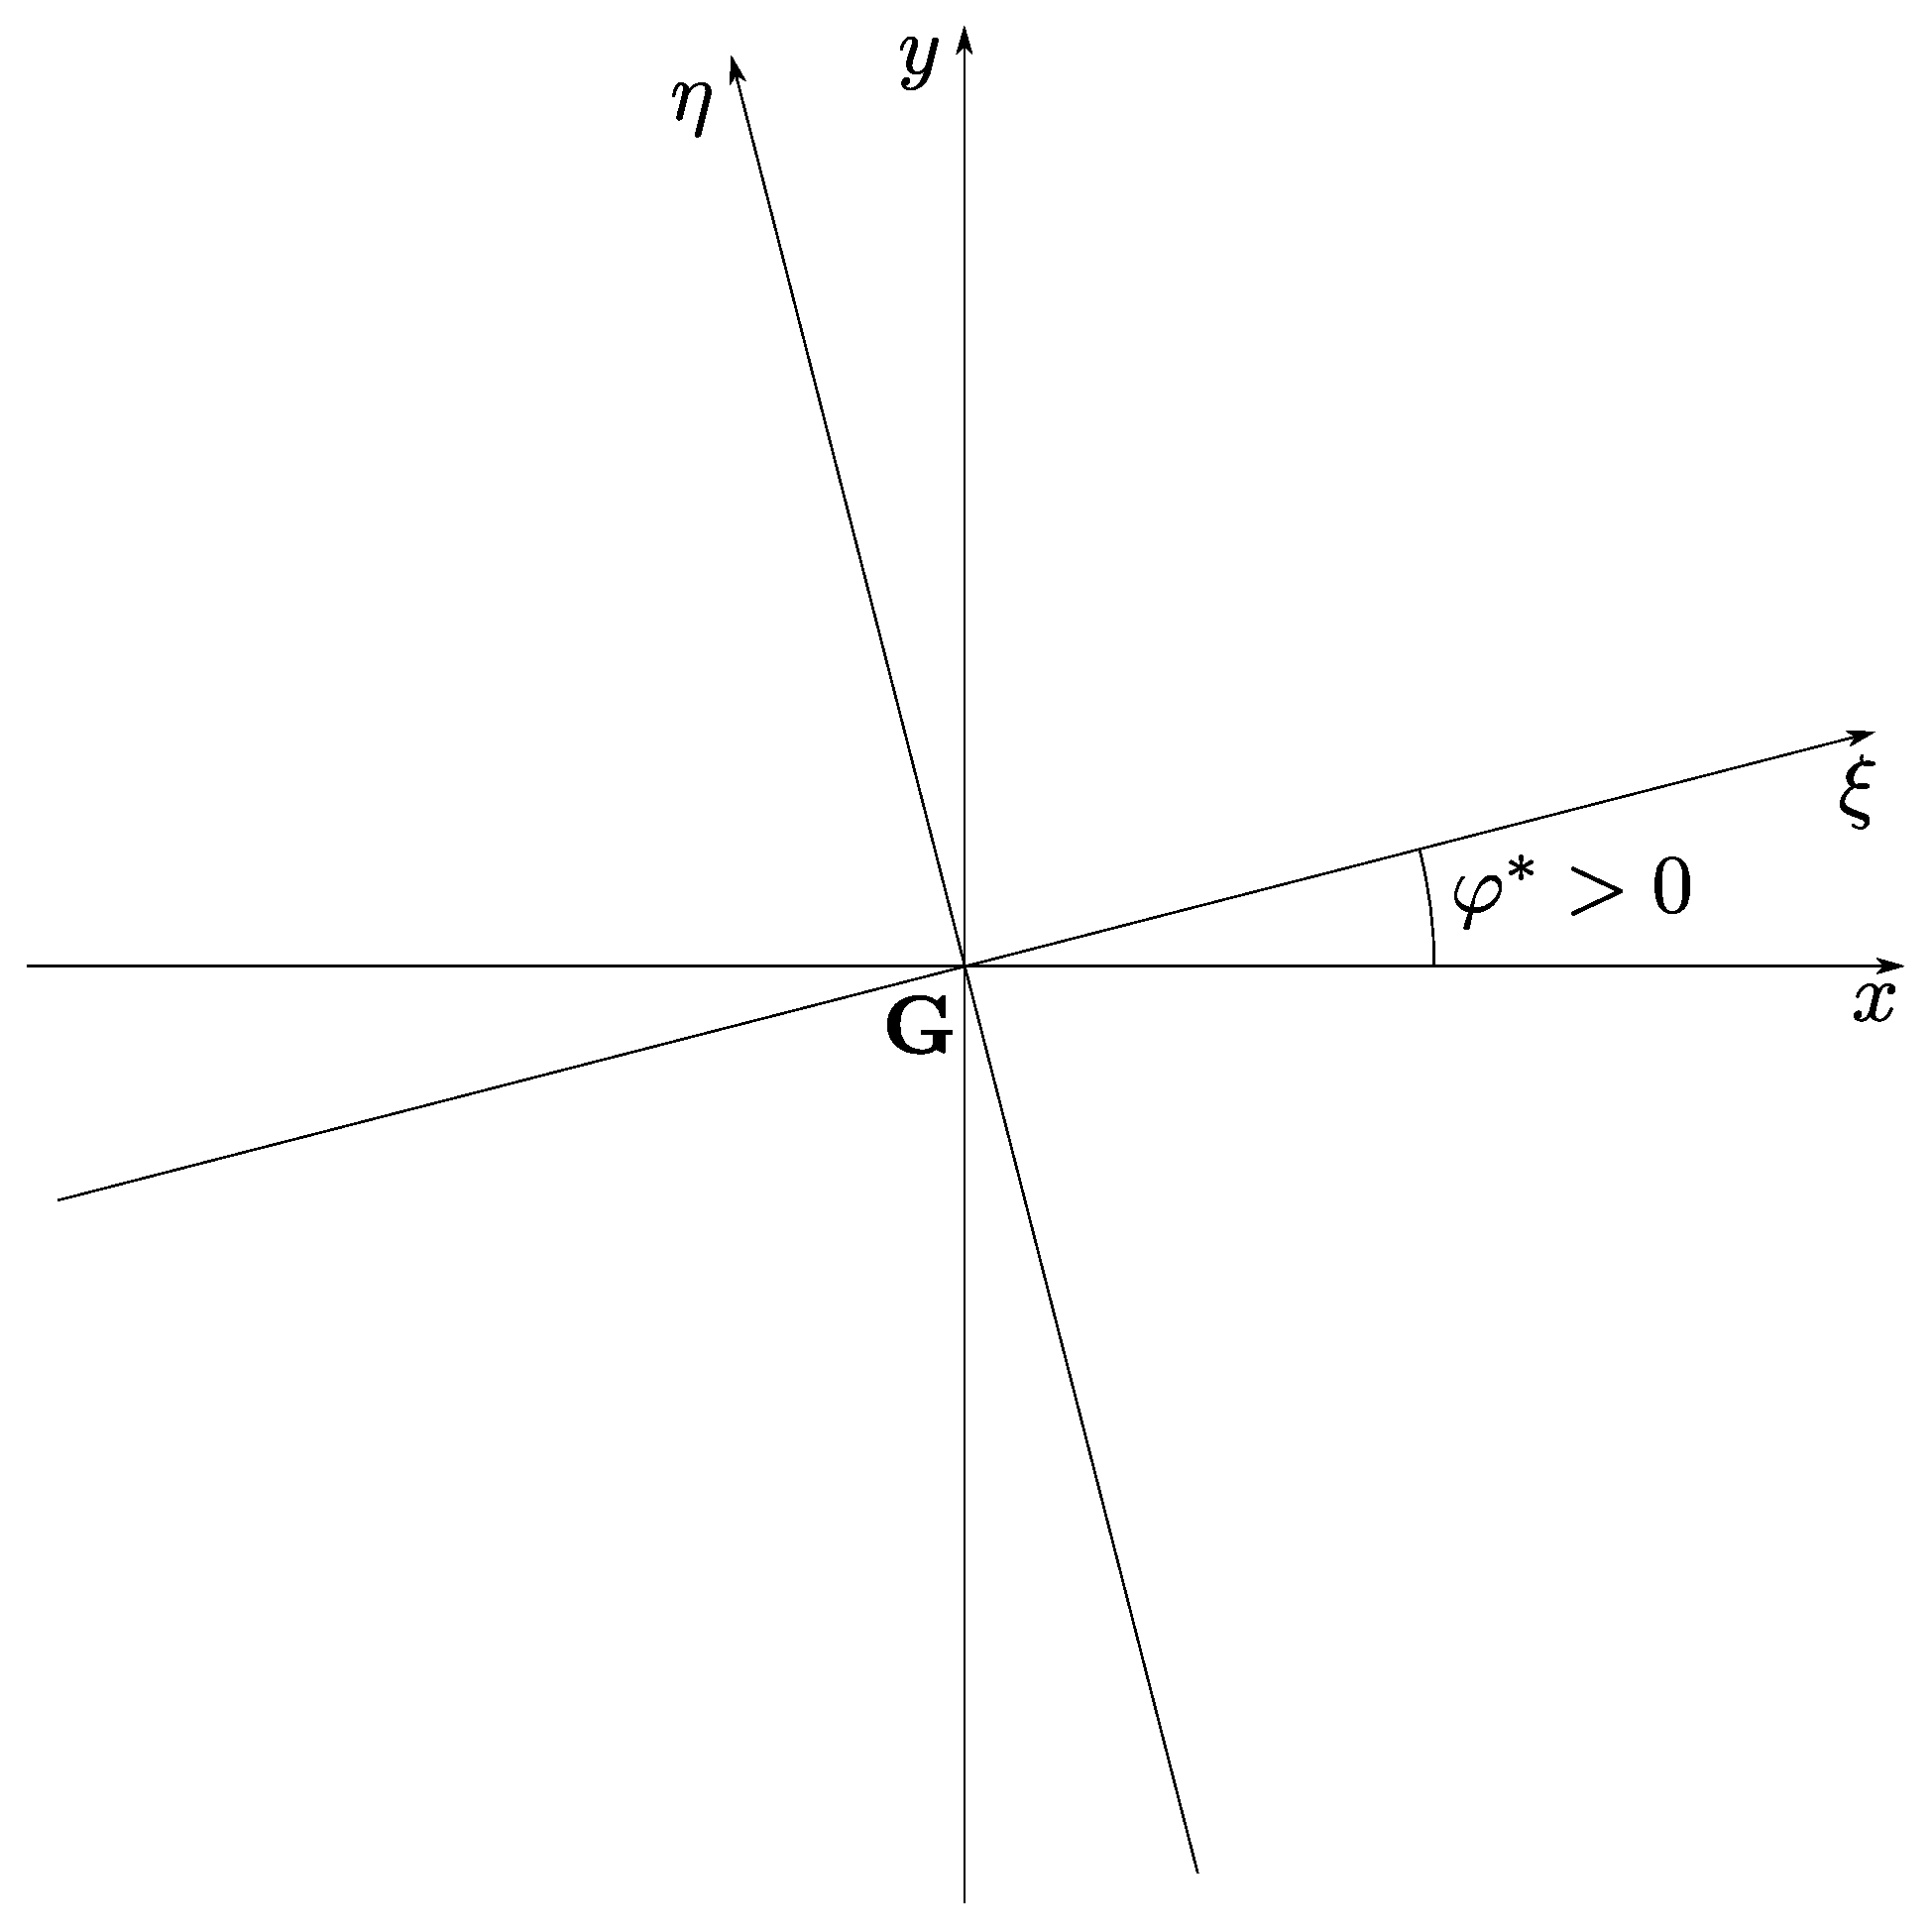
\includegraphics[width=0.65\textwidth]{Immagini/Parte_4/Figura4_2/Figura4_2.pdf}
\caption{}
\label{figura4-2}
\end{figure}
%--------------------------------------------------------------------------------------------------------------------------------------------------------------
\noindent Le equazioni~\eqref{equazione4-1} sono valide qualunque sia l'origine degli assi, ferme restando le precisazioni già fatte (si veda l'elenco della pagina precedente); naturalmente, esse acquistano la massima importanza allorché l'origine degli assi coincide con il baricentro. 

\noindent In ogni caso, dalle~\eqref{equazione4-1}, con semplici passaggi, si trae
%--------------------------------------------------------------------------------------------------------------------------------------------------------------
\begin{align*}
\frac{dI_{x'}}{d\varphi} &= -2I_{x'y'} \\
\frac{dI_{y'}}{d\varphi} &= +2I_{x'y'}
\end{align*}
%--------------------------------------------------------------------------------------------------------------------------------------------------------------
Da ciò scaturisce la seguente, notevole, proposizione
%--------------------------------------------------------------------------------------------------------------------------------------------------------------
\begin{quoting}
Tra gli infiniti riferimenti con origine in $\mathbf{G}$ ve ne è uno particolarmente importante, che indicheremo con $\mathbf{G}\xi\eta$. Si tratta di quel riferimento rispetto a cui è nullo il momento centrifugo e conseguentemente, i \textsc{momenti di inerzia} sono uno \textsc{minimo} e l'altro \textsc{massimo}.
\end{quoting}
%--------------------------------------------------------------------------------------------------------------------------------------------------------------
Le rette $\xi$ ed $\eta$ si dicono \textsc{assi principali di inerzia} della figura piana in esame. Esse sono baricentriche, ortogonali, e caratterizzate, come già detto, dalle condizioni seguenti
%--------------------------------------------------------------------------------------------------------------------------------------------------------------
\begin{align*}
I_{\xi} &= I_{\textup{max}}\,\textup{oppure}\,I_{\textup{min}} \\
I_{\eta} &= I_{\textup{max}}\,\textup{oppure}\,I_{\textup{min}} \\
I_{\xi\eta} &= 0
\end{align*}
%--------------------------------------------------------------------------------------------------------------------------------------------------------------
Dalla terza delle~\eqref{equazione4-1}, uguagliando a zero $I_{x'y'}$ si trova
%--------------------------------------------------------------------------------------------------------------------------------------------------------------
\begin{equation} \label{equazione4-2}
\boxed{\tan 2\varphi^* = \frac{2I_{xy}}{I_{y}-I_{x}}}
\tag{4.2}
\end{equation}
%--------------------------------------------------------------------------------------------------------------------------------------------------------------
Il valore di $\varphi^*$ che si ricava dalla~\eqref{equazione4-2} è l'angolo che $\xi$ forma con $x$; qualunque calcolatrice fornirà un valore di $2\varphi^*$ compreso fra $-90^{\circ}$ e $+90^{\circ}$; e quindi
%--------------------------------------------------------------------------------------------------------------------------------------------------------------
\begin{equation*}
\boxed{-45^{\circ}\le \varphi^{*} \le 45^{\circ}}
\end{equation*}
%--------------------------------------------------------------------------------------------------------------------------------------------------------------
La figura~\ref{figura4-2} mostra la corretta interpretazione grafica dell'asse $\xi$  e, conseguentemente, dell'asse $\eta$. Noto $\varphi^{*}$, è agevole calcolare $I_{\xi}$ ed $I_{\eta}$: basterà utilizzare le prime due delle~\eqref{equazione4-1} identificando $x'$ con $\xi$ ed $y'$ con $\eta$ e ponendo $\varphi^{*}$ al posto di $\varphi$. 

\noindent Noi sappiamo che
%--------------------------------------------------------------------------------------------------------------------------------------------------------------
\begin{equation*}
\boxed{r\textup{\textsc{ asse di simmetria (ortogonale o no) rispetto a }}\delta} \longrightarrow \boxed{I_{rs} = 0, \quad \forall\,s\parallelsum\,\delta}
\end{equation*}
%--------------------------------------------------------------------------------------------------------------------------------------------------------------
Ebbene, alla luce di quest'ultima proposizione, appaiono evidenti le seguenti:
%--------------------------------------------------------------------------------------------------------------------------------------------------------------
\begin{equation*}
\boxed{\textup{\scriptsize \textsc{Se una figura piana ha }}2\textup{\scriptsize \textsc{ assi di simmetria ortogonali, questi sono assi principali di inerzia}}}
\end{equation*}
%--------------------------------------------------------------------------------------------------------------------------------------------------------------
\begin{equation*}
\boxed{\textup{\scriptsize \textsc{Se una figura piana ha }}1\textup{\scriptsize \textsc{ asse di simmetria ortogonale, questo è asse principale di inerzia}}}
\end{equation*}
%--------------------------------------------------------------------------------------------------------------------------------------------------------------
Nel caso della seconda proposizione, l'altro asse è ovviamente ortogonale al primo e passante per $\mathbf{G}$.
%--------------------------------------------------------------------------------------------------------------------------------------------------------------
\clearpage
\section{Esercizi}
\paragraph{Esercizio 4.1}
Determinare gli assi principali di inerzia e calcolare i relativi momenti di inerzia per il profilato in figura.
%--------------------------------------------------------------------------------------------------------------------------------------------------------------
\renewcommand{\thefigure}{4.1~-~1}
\begin{figure}[ht]
\centering
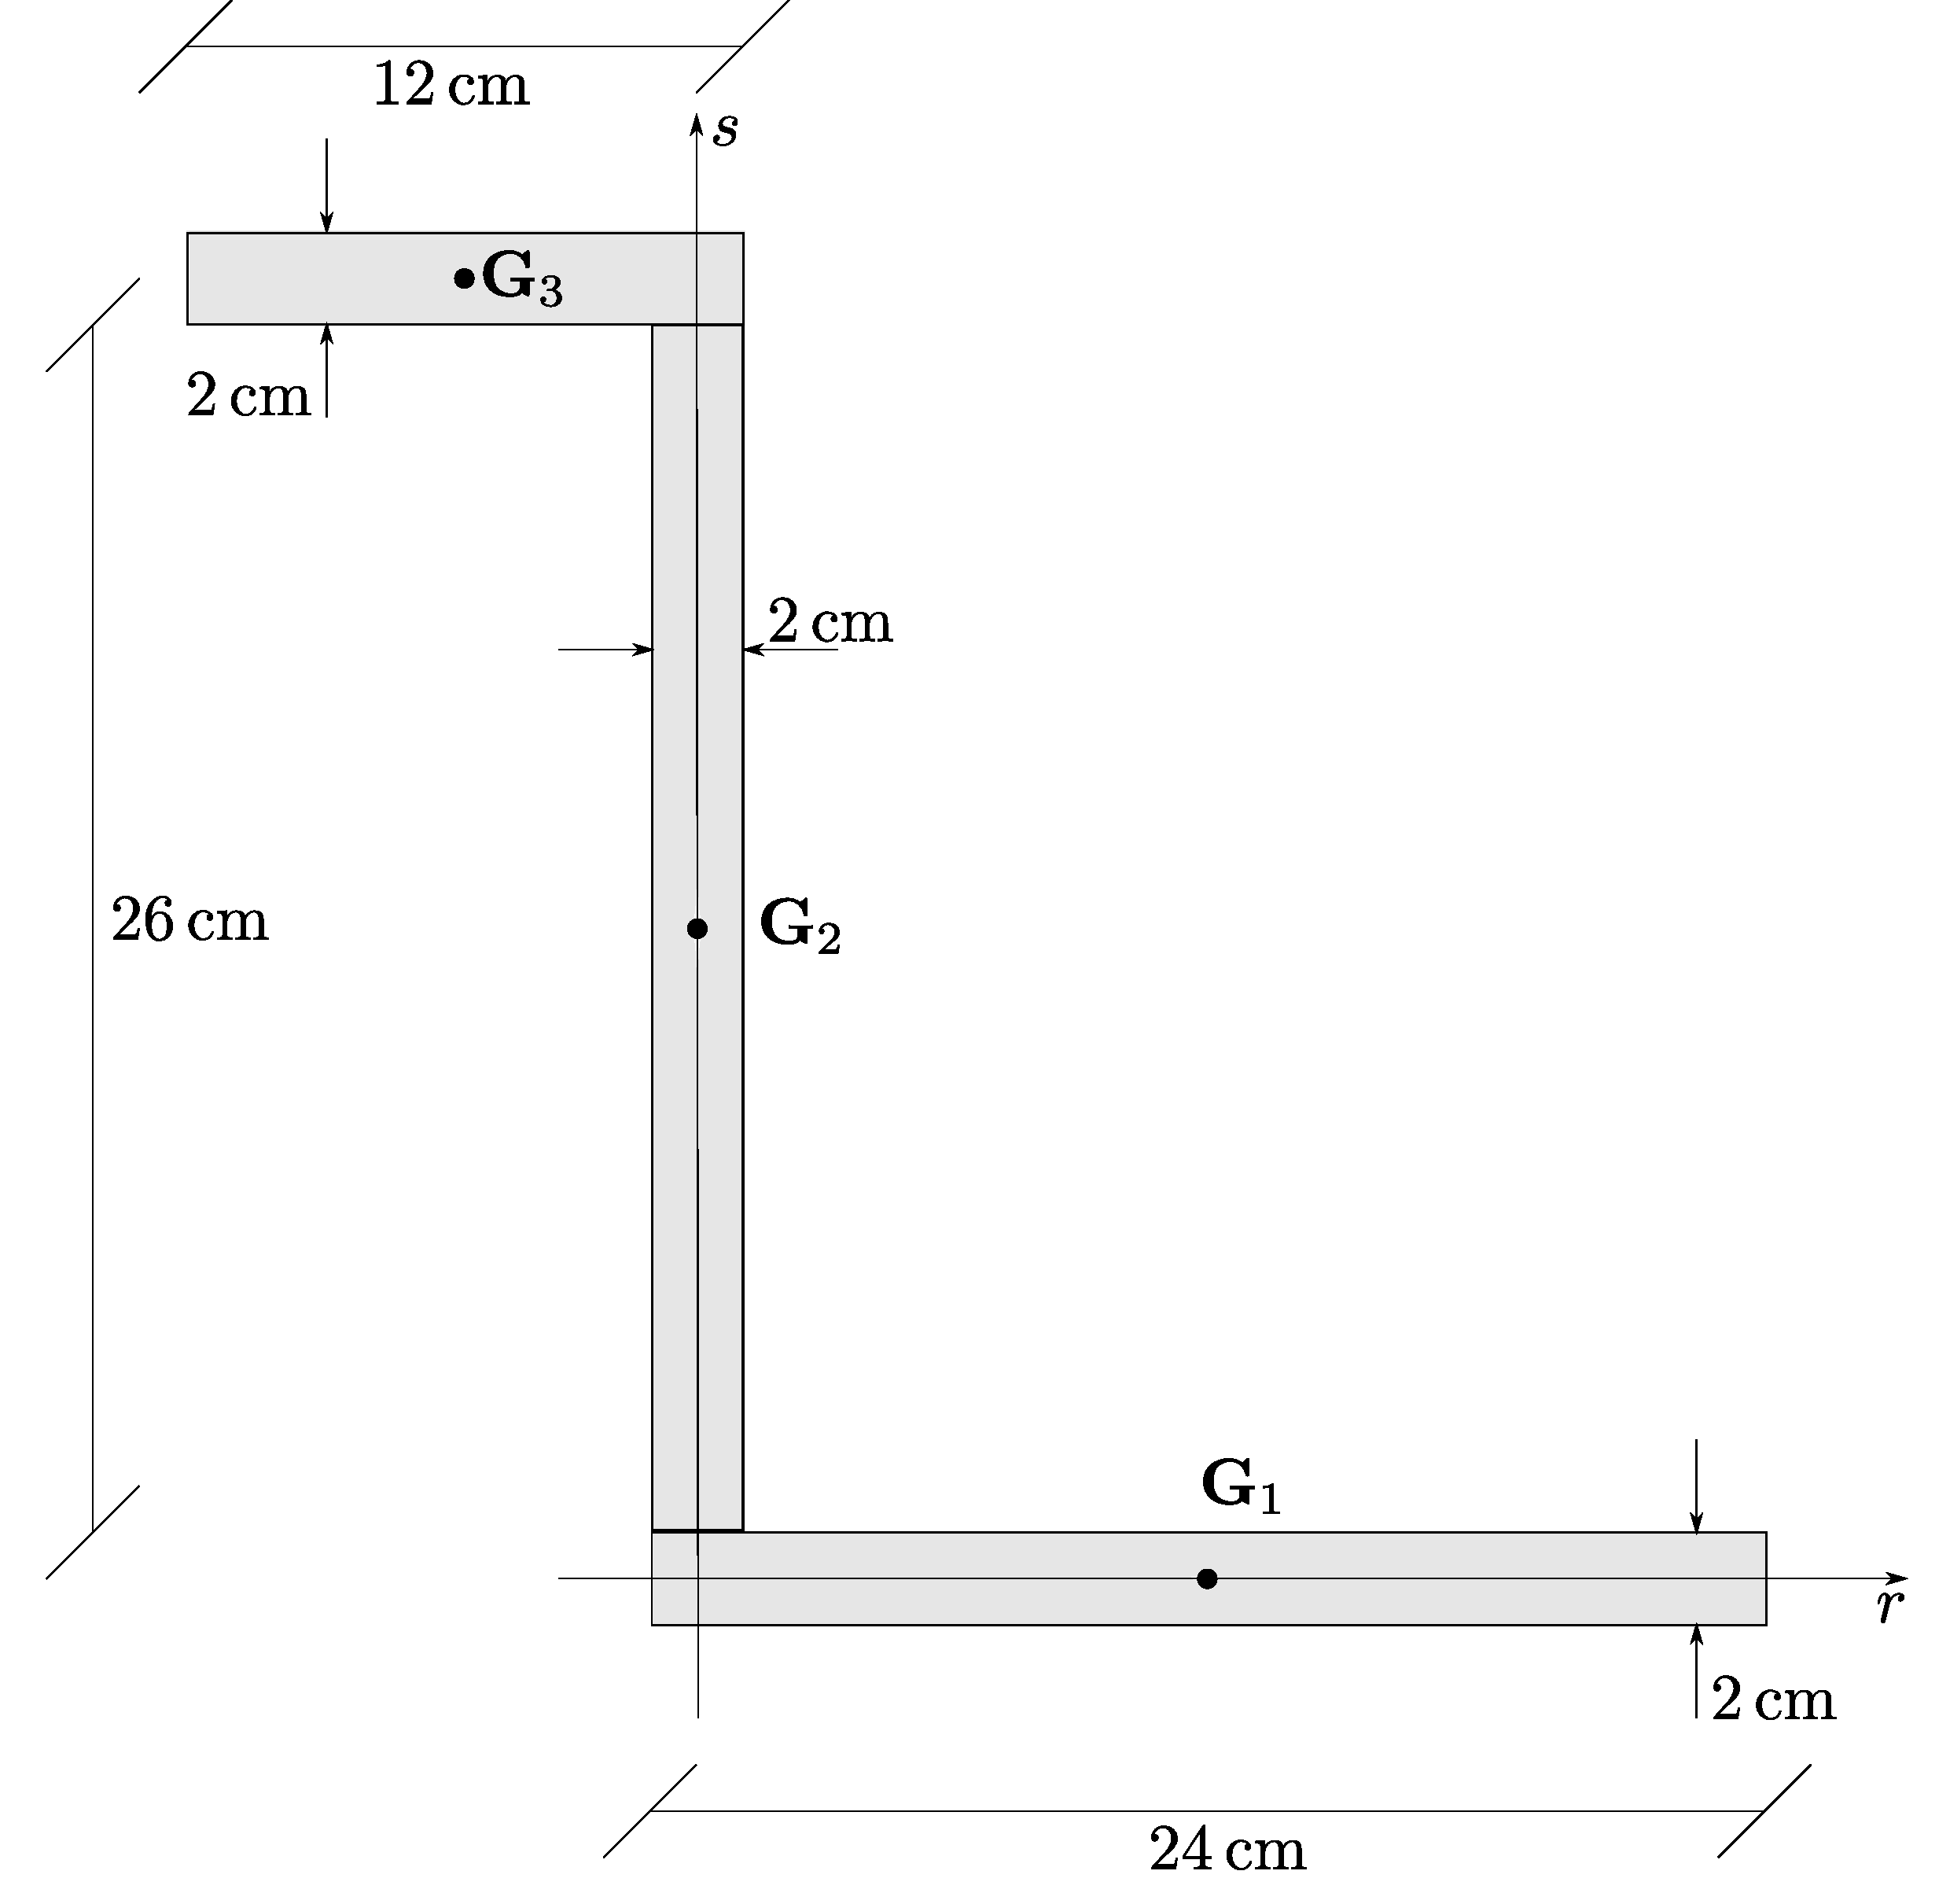
\includegraphics[width=0.8\textwidth]{Immagini/Parte_4/Esercizio4_1/Esercizio4_1_1.pdf}
\caption{}
\label{Esercizio4-1-1}
\end{figure}
%--------------------------------------------------------------------------------------------------------------------------------------------------------------

\noindent Cominciamo a determinare $\mathbf{G}$ 
%----------------------------------------------------------------------------------------
\begin{equation*}
\begin{aligned}
A_1 &= 48\,\textup{cm}^2 \\
A_2 &= 52\,\textup{cm}^2 \\
A_3 &= 24\,\textup{cm}^2
\end{aligned}
\,\,\Biggr\}\,\, A = 124\,\textup{cm}^2
\end{equation*}
%----------------------------------------------------------------------------------------
%----------------------------------------------------------------------------------------
\begin{equation*}
\begin{aligned}
S_{1r} &= 0\,\textup{cm}^3 \\
S_{2r} &= 54\times 14 = 728\,\textup{cm}^3 \\
S_{3r} &= 24\times 28  = 672\,\textup{cm}^3
\end{aligned}
\,\,\Biggr\}\,\, S_r = 1400\,\textup{cm}^3
\end{equation*}
%----------------------------------------------------------------------------------------
%----------------------------------------------------------------------------------------
\begin{equation*}
\begin{aligned}
S_{1s} &= 48\times 11 = 528\,\textup{cm}^3 \\
S_{2s} &= 0 \\
S_{3s} &= 24\times (-5)  = -120\,\textup{cm}^3
\end{aligned}
\,\,\Biggr\}\,\, S_r = 408\,\textup{cm}^3
\end{equation*}
%----------------------------------------------------------------------------------------
\begin{align*}
\lambda_{rG} &= \frac{S_r}{A} = \frac{1400}{124} = 11.29\,\textup{cm} \\
\lambda_{sG} &= \frac{S_s}{A} = \frac{408}{124} = 3.29\,\textup{cm}
\end{align*}
%----------------------------------------------------------------------------------------
%--------------------------------------------------------------------------------------------------------------------------------------------------------------
\renewcommand{\thefigure}{4.1~-~2}
\begin{figure}[ht]
\centering
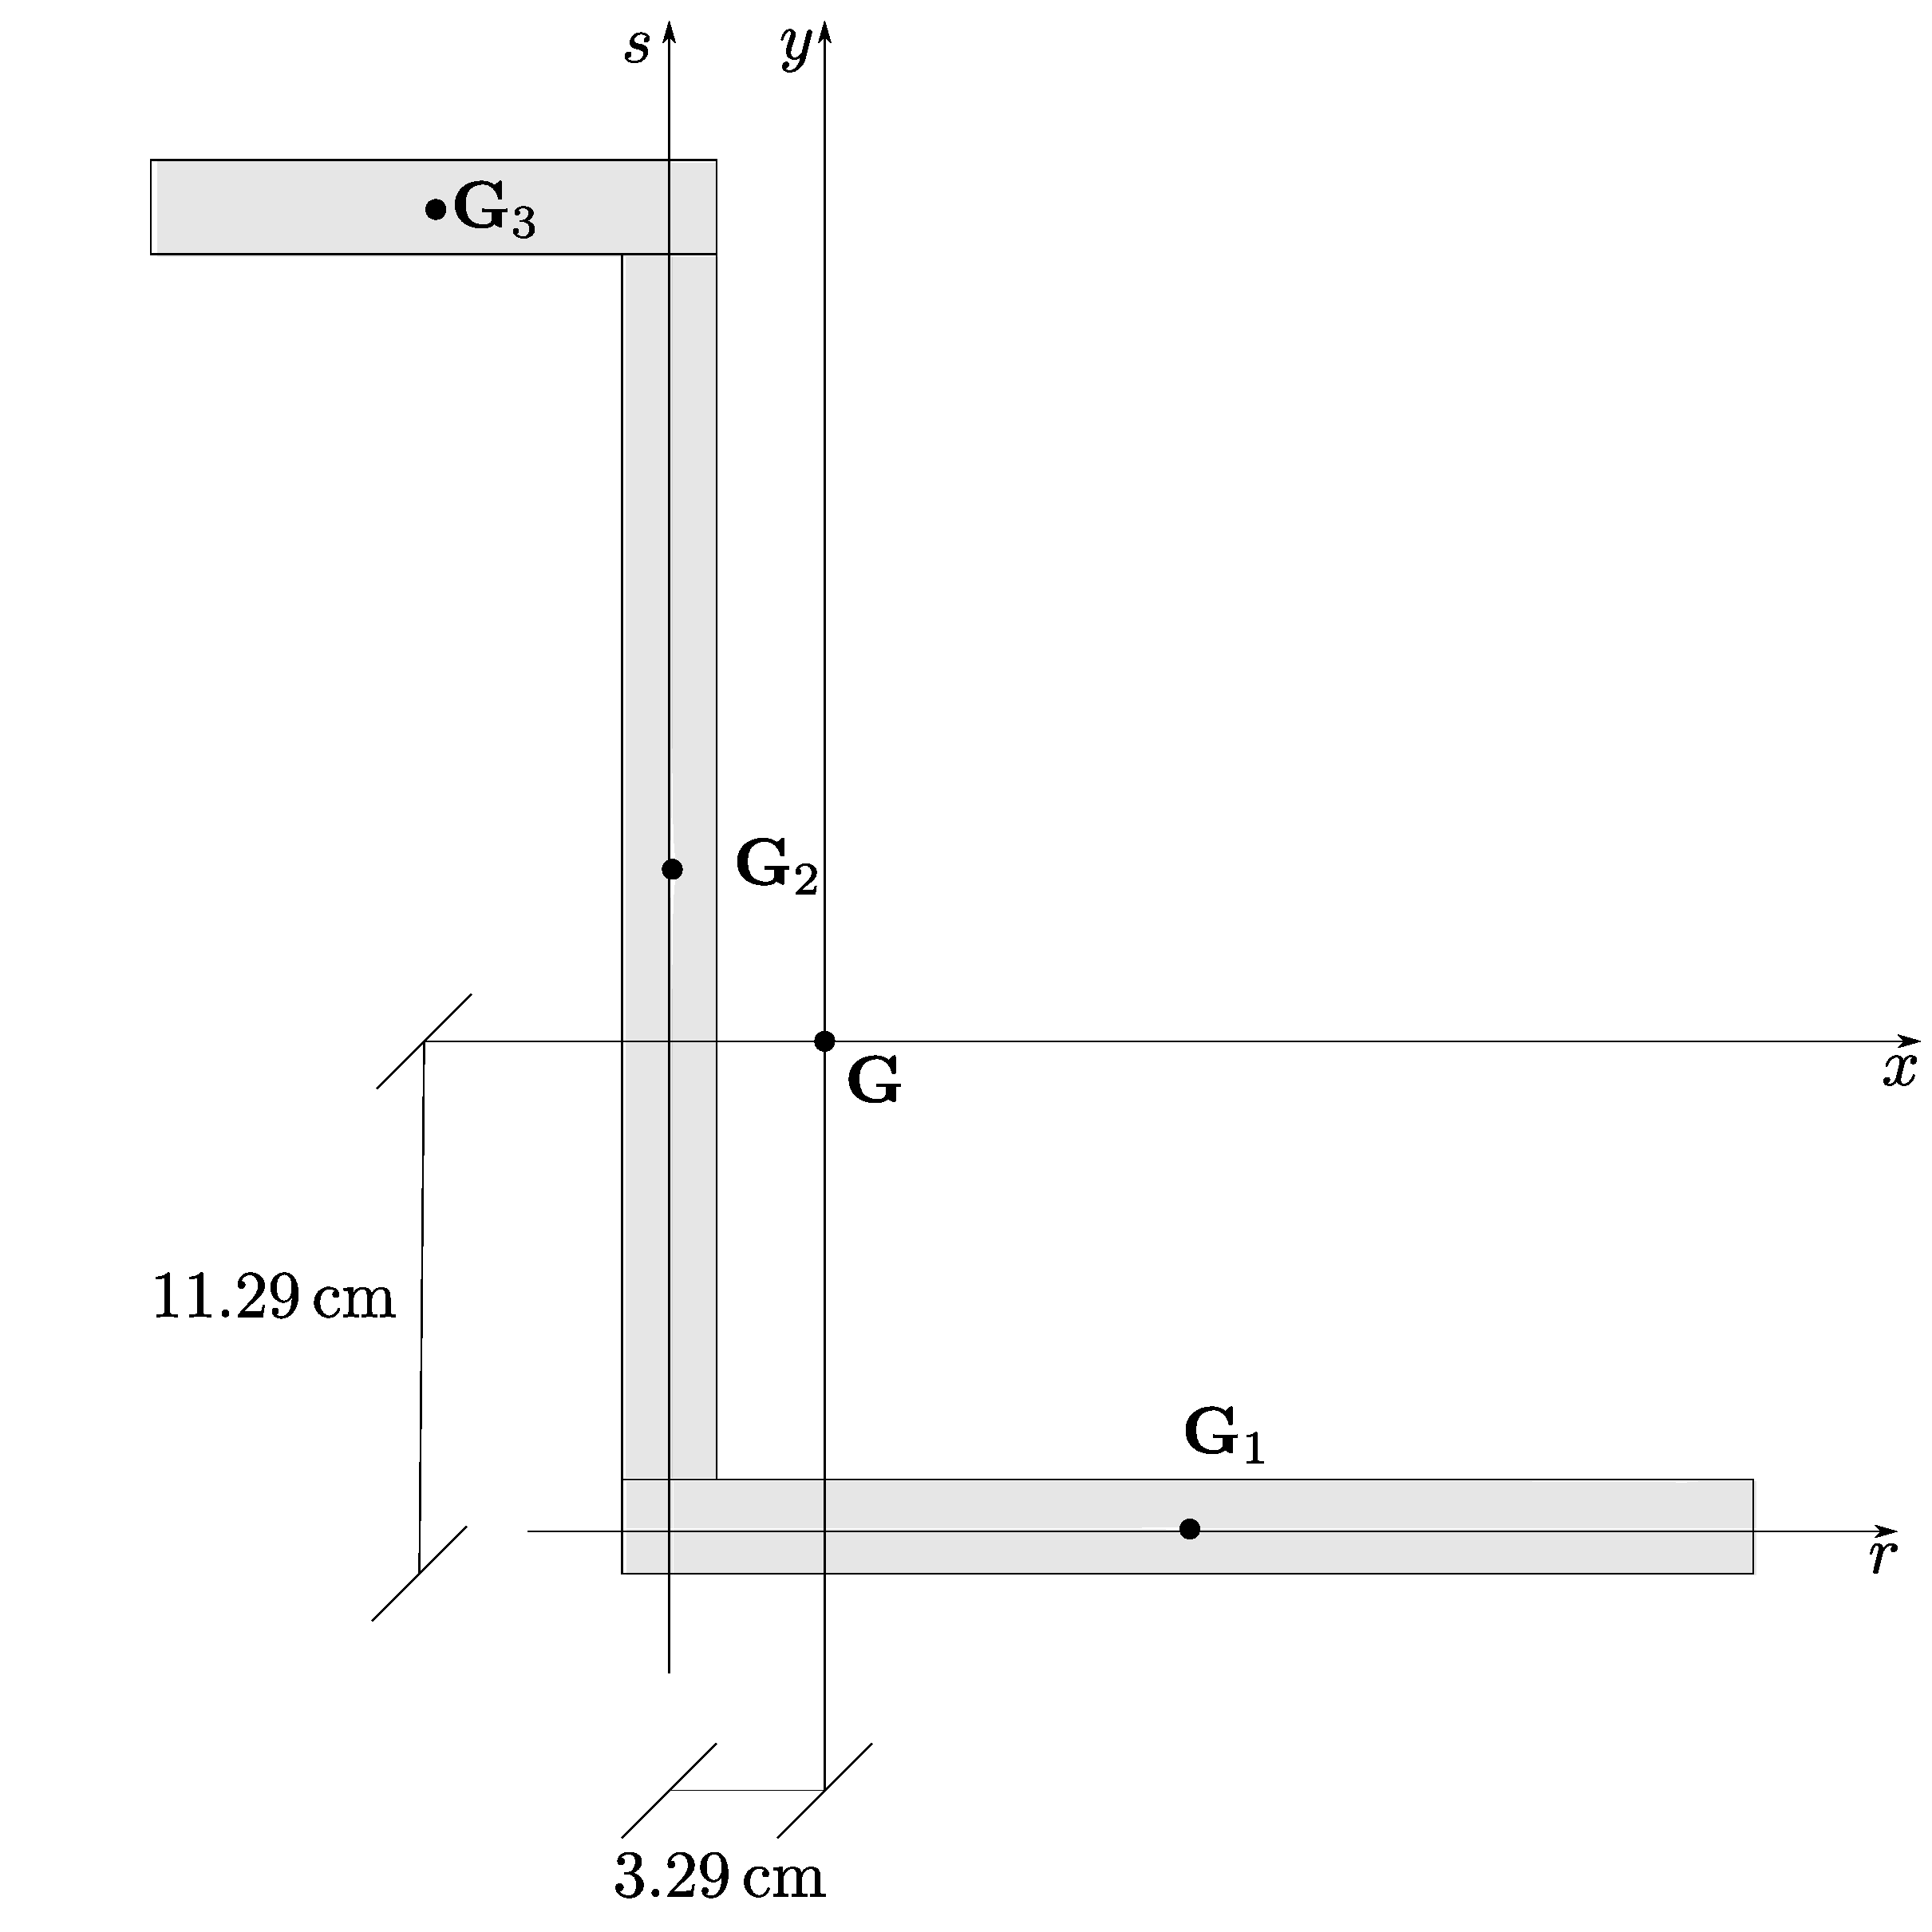
\includegraphics[width=0.8\textwidth]{Immagini/Parte_4/Esercizio4_1/Esercizio4_1_2.pdf}
\caption{}
\label{Esercizio4-1-2}
\end{figure}
%--------------------------------------------------------------------------------------------------------------------------------------------------------------

\noindent Abbiamo ridisegnato il profilato con gli assi $x$ ed $y$ paralleli ai lati dei rettangoli: questi sono, ovviamente, fra tutti gli assi baricentrici, quelli per cui è più agevole calcolare $I_x$, $I_y$ ed $I_{xy}$. Conviene comunque calcolare prima $I_r$, $I_s$ ed $I_{rs}$ per poi ricavare, applicando i teoremi del trasporto $I_x$, $I_y$ ed $I_{xy}$.
%----------------------------------------------------------------------------------------
\begin{equation*}
\begin{aligned}
I_{1r} &= \frac{24\times 2^3}{12} = 16\,\textup{cm}^4 \\
I_{2r} &= \frac{2\times 26^3}{12} + 52\times 14^2 = 13121\,\textup{cm}^4  \\
I_{3r} &= \frac{12\times 2^3}{12} + 24\times 28^2 = 18824\,\textup{cm}^4
\end{aligned}
\,\,\Biggr\}\,\, I_r = 31961\,\textup{cm}^4
\end{equation*}
%----------------------------------------------------------------------------------------
%----------------------------------------------------------------------------------------
\begin{equation*}
\begin{aligned}
I_{1s} &= \frac{2\times 26^3}{12} + 48\times 11^2 = 8112\,\textup{cm}^4 \\
I_{2s} &= \frac{26\times 2^3}{12} = 17\,\textup{cm}^4 \\
I_{3s} &= \frac{2\times 12^3}{12} + 24\times 5^2 = 888\,\textup{cm}^4
\end{aligned}
\,\,\Biggr\}\,\, I_s = 9017\,\textup{cm}^4
\end{equation*}
%----------------------------------------------------------------------------------------
%----------------------------------------------------------------------------------------
\begin{equation*}
\begin{aligned}
I_{1rs} &= 0 \\
I_{2rs} &= 0 \\
I_{3rs} &= 24\times(-5)\times 28 = -3360\,\textup{cm}^4
\end{aligned}
\,\,\Biggr\}\,\, I_{rs} = -3360\,\textup{cm}^4
\end{equation*}
%----------------------------------------------------------------------------------------
Ed ora possiamo calcolare $I_x$, $I_y$ ed $I_{xy}$
%----------------------------------------------------------------------------------------
\begin{align*}
I_{x} &= I_{r}-Ay_{G}^{2} = 31961-124\times 11.29^{2} = 16155\,\textup{cm}^4 \\
I_{y} &= I_{s}-Ax_{G}^{2} = 9017-124\times 3.29^{2} = 7675\,\textup{cm}^4  \\
I_{xy} &= I_{rs}-Ay_{G}x_{G} = -3360-124\times 11.29\times 3.29 = -7966\,\textup{cm}^4
\end{align*}
%----------------------------------------------------------------------------------------
A questo punto, applicando le~\eqref{equazione4-2}, possiamo calcolare l'angolo $\varphi^{*}$ che $\xi$ forma con $x$
%----------------------------------------------------------------------------------------
\begin{equation*}
\tan 2\varphi^{*} = \frac{2I_{xy}}{I_{y}-I_{x}} = -\frac{2\times 7966}{7675-16155} = 1.87877
\end{equation*}
%----------------------------------------------------------------------------------------
Quindi
%----------------------------------------------------------------------------------------
\begin{equation*}
2\varphi^{*} = 62^{\circ} \longrightarrow \varphi^{*} = 31^{\circ}
\end{equation*}
%--------------------------------------------------------------------------------------------------------------------------------------------------------------
\renewcommand{\thefigure}{4.1~-~3}
\begin{figure}[ht]
\centering
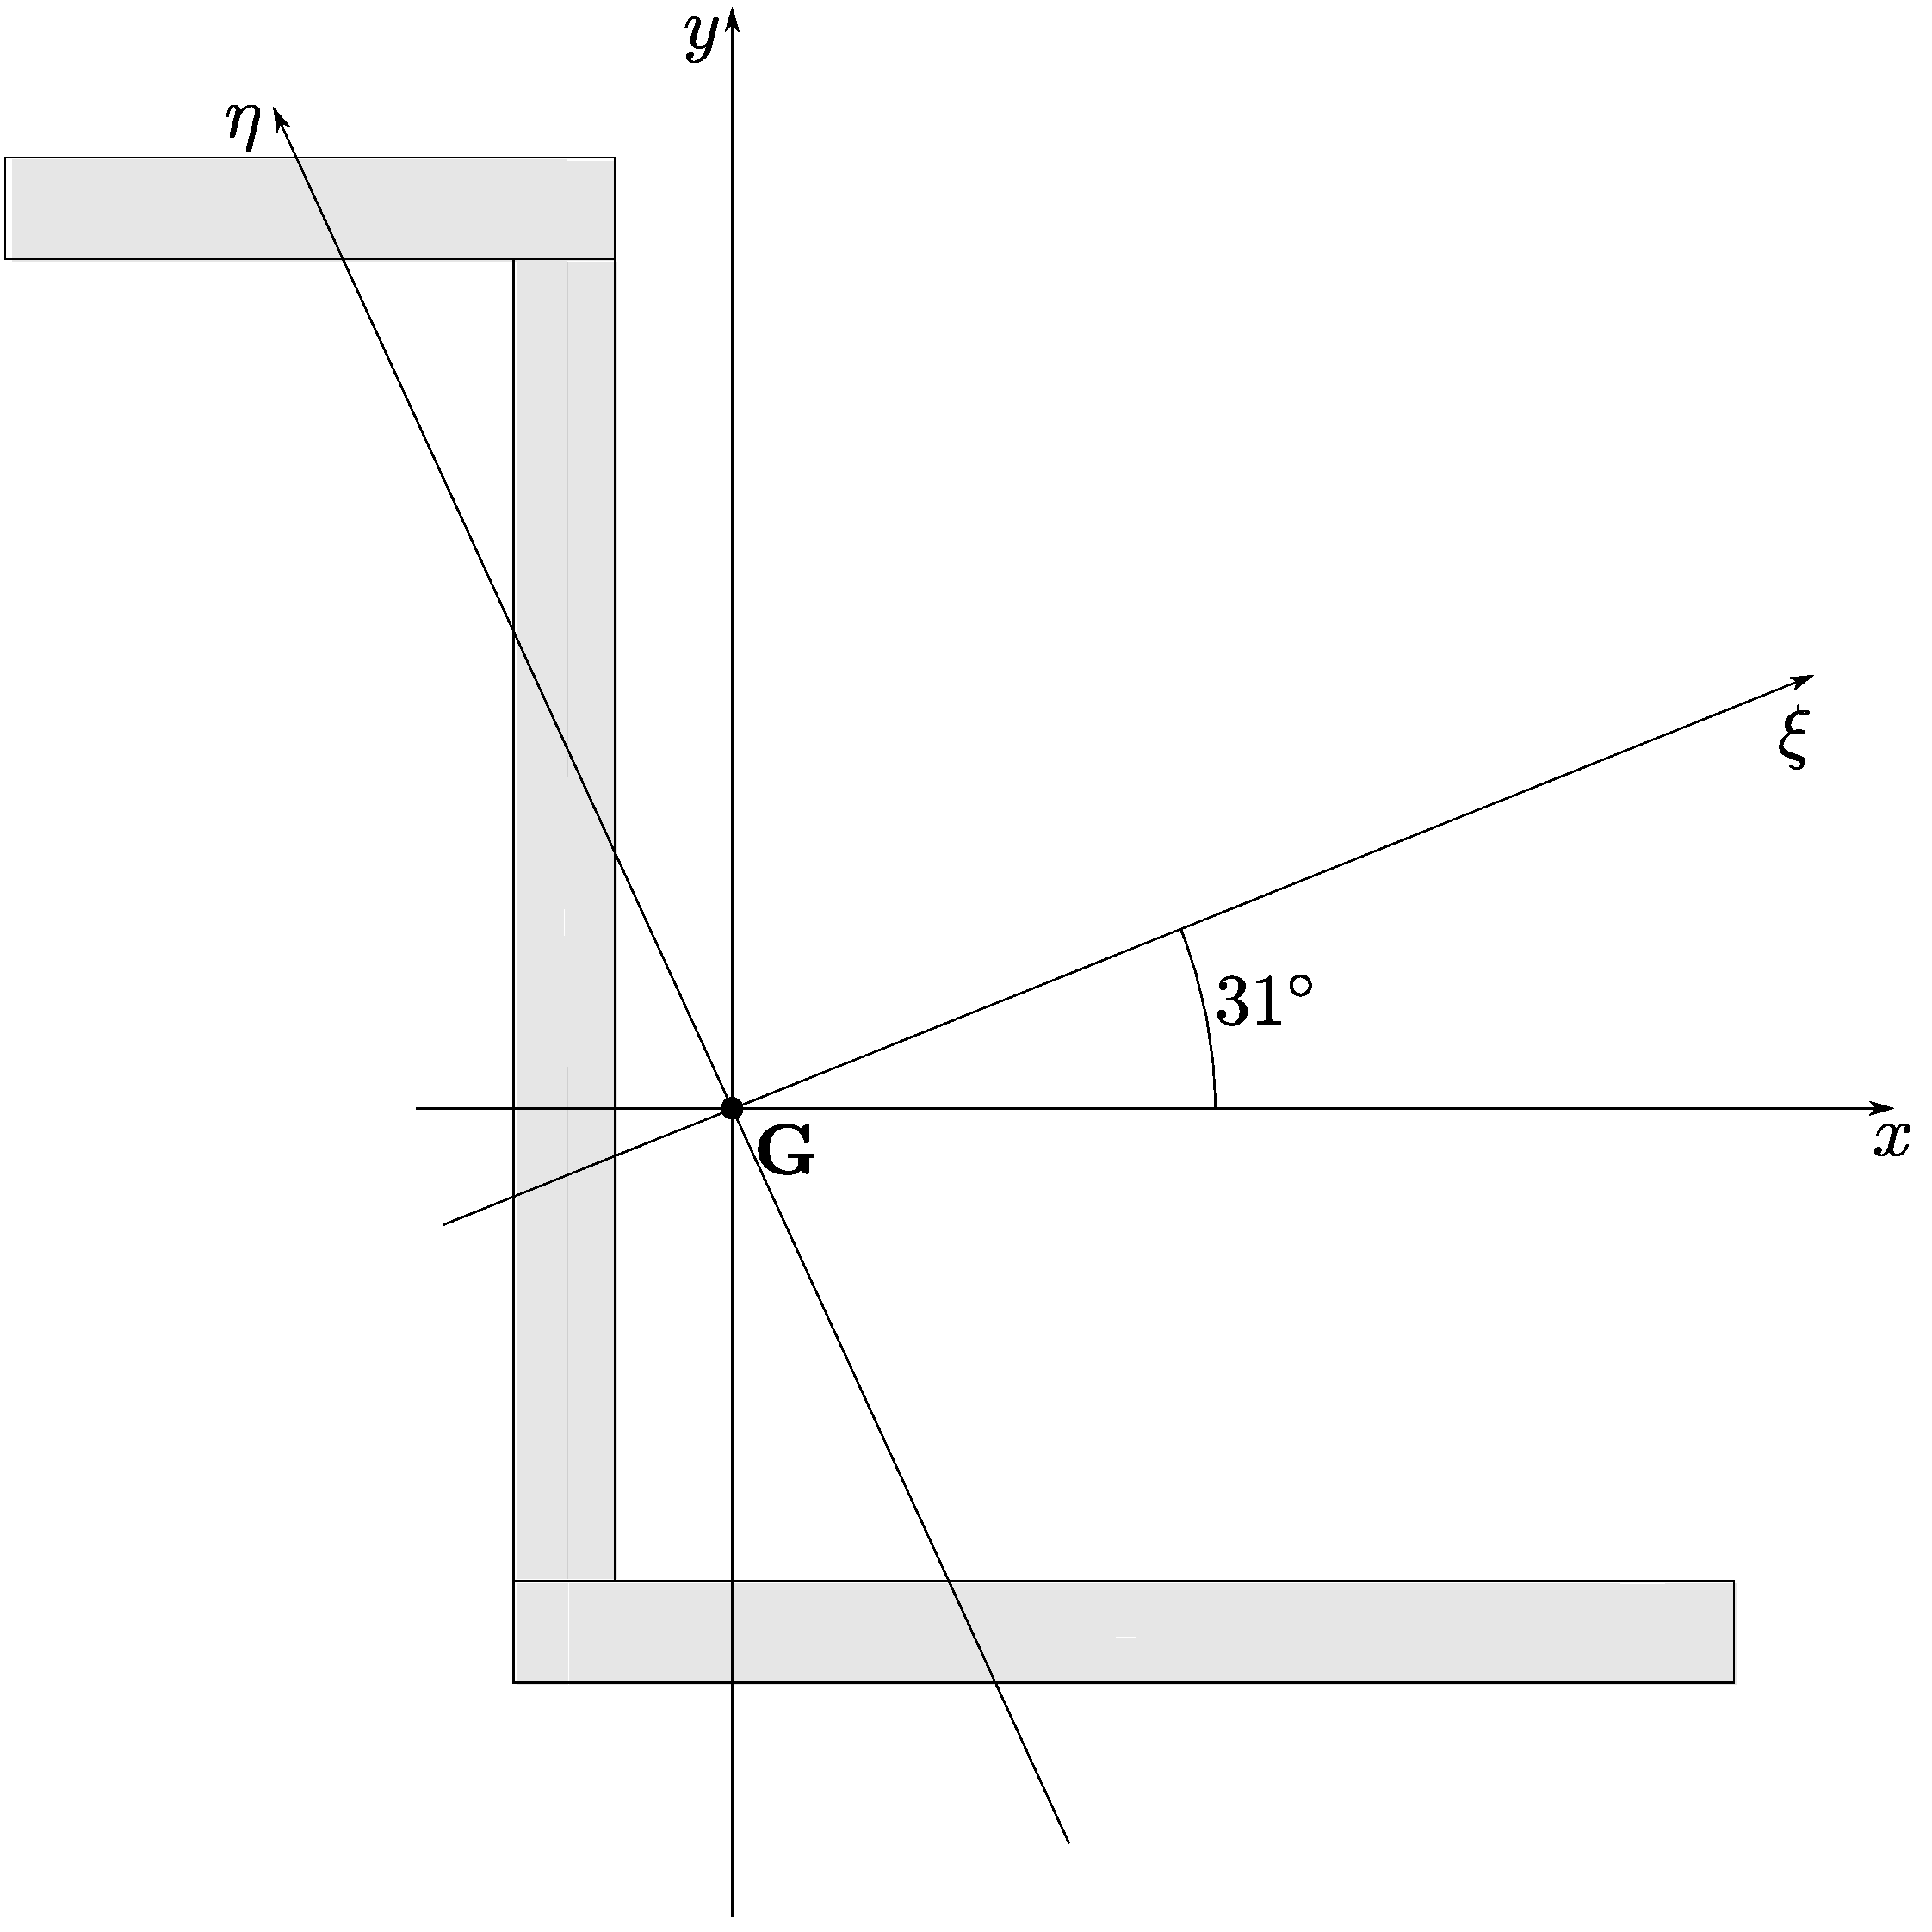
\includegraphics[width=\textwidth]{Immagini/Parte_4/Esercizio4_1/Esercizio4_1_3.pdf}
\caption{}
\label{Esercizio4-1-3}
\end{figure}
%--------------------------------------------------------------------------------------------------------------------------------------------------------------
Calcoleremo $I_{\xi}$ ed $I_{\eta}$ ponendo $\varphi=31^{\circ}$ rispettivamente nella prima e nella seconda delle~\eqref{equazione4-1}
%----------------------------------------------------------------------------------------
\begin{align*}
I_{\xi} &= 16155\times\cos^{2}31^{\circ}+7675\times\sin^{2}31^{\circ}+7966\times\sin^{2}62^{\circ} = 20939\,\textup{cm}^4 \\
I_{\eta} &= 16155\times\sin^{2}31^{\circ}+7675\times\cos^{2}31^{\circ}-7966\times\sin^{2}62^{\circ} = 2891\,\textup{cm}^4
\end{align*}
%----------------------------------------------------------------------------------------
La situazione finale ottenuta dal calcolo appena fatto è rappresentata in figura alla pagina seguente.
%----------------------------------------------------------------------------------------
%------------------------------------------------
\clearpage
\pagestyle{fancy}
\part{Il cerchio di Mohr}
\setcounter{section}{0}
\section{La costruzione del cerchio di Mohr}
%----------------------------------------------------------------------------------------
\renewcommand{\thefigure}{5~-~1}
\begin{figure}[h]
\centering
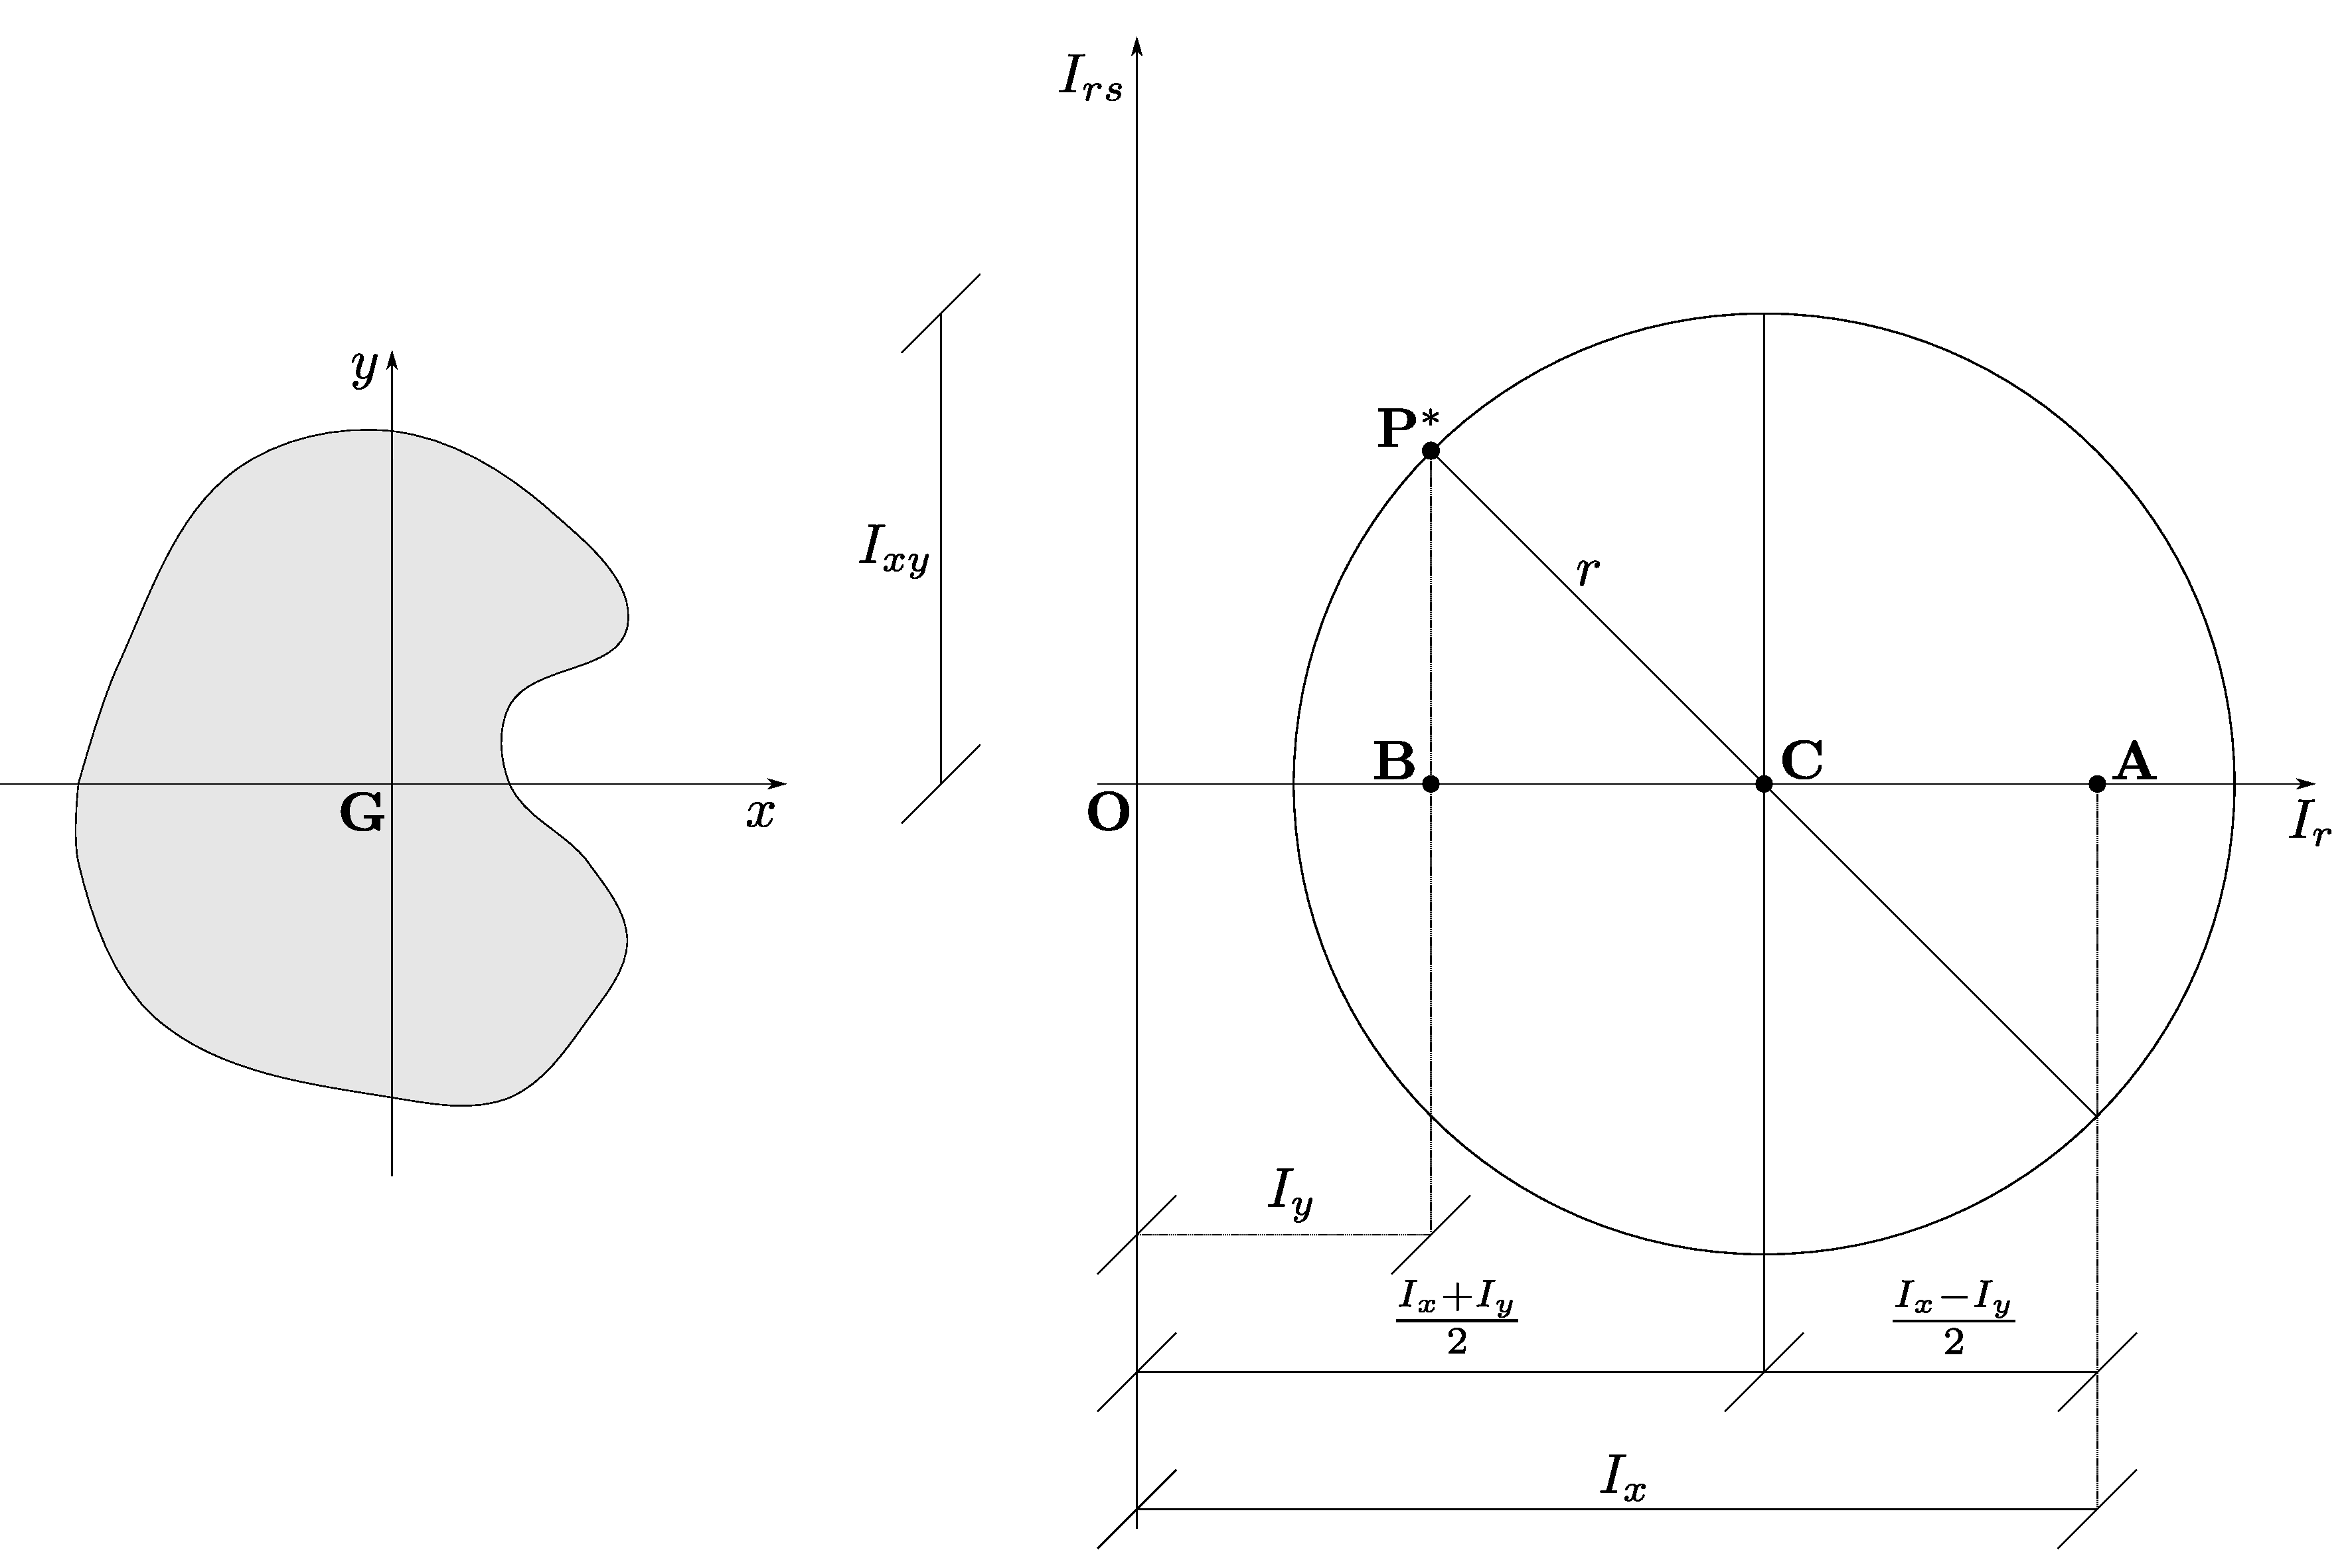
\includegraphics[width=\textwidth]{Immagini/Parte_5/Figura5_1/Figura5_1.pdf}
\caption{}
\label{figura5-1}
\end{figure}
%----------------------------------------------------------------------------------------
%--------------------------------------------------------------------------------------------------------------------------------------------------------------
\noindent Noti $I_x$, $I_y$ ed $I_{xy}$ di una data figura piana, l'origine del riferimento esendo in $\mathbf{G}$, abbiamo visto come sia possibile, grazie alla~\eqref{equazione4-2}, determinare gli assi principali $\xi$ ed $\eta$ e, grazie alle prime due delle~\eqref{equazione4-2}, calcolare $I_{\xi}$ ed $I_{\eta}$. 

\noindent Ebbene il \textsc{cerchio di Mohr} costituisce un'alternativa grafica al suddetto procedimento analitico. Noti $I_x$, $I_y$ ed $I_{xy}$ della figura piana in questione, per costruire il cerchio di Mohr si procede come segue (si faccia riferimento alla figura~\ref{figura5-1}):
%--------------------------------------------------------------------------------------------------------------------------------------------------------------
\begin{enumerate}
\item si disegnano, con origine arbitraria, le due rette $I_r$ ed $I_{rs}$ parallele e concordi ad $x$ ed $y$;
\item si assume (a piacere) una scala che traduca in $[\textup{cm}]$ i valori di $I_x$, $I_y$ ed $I_{xy}$;
\item nel riferimento $\mathbf{O}I_{r}I_{rs}$ si evidenziano i punti 
%--------------------------------------------------------------------------------------------------------------------------------------------------------------
\begin{align*}
&\mathbf{A}(I_{x},\,0) \\
&\mathbf{B}(I_{y},\,0) \\
&\mathbf{P}^{*}(I_{y},\,I_{xy}) 
\end{align*}
%--------------------------------------------------------------------------------------------------------------------------------------------------------------
\item si evidenzia il punto $\mathbf{C}$ medio del segmento $\mathbf{AB}$, la cui ascissa è ovviamente 
%--------------------------------------------------------------------------------------------------------------------------------------------------------------
\begin{equation*}
\lvert \, \mathbf{OC} \, \lvert = \frac{I_{x}+I_{y}}{2}
\end{equation*}
%--------------------------------------------------------------------------------------------------------------------------------------------------------------
\item si traccia la circonferenza di centro $\mathbf{C}$ e raggio $r=\lvert\,\mathbf{C}\mathbf{P}^{*}\lvert$: si è così costruito il cerchio di Mohr relativo alla figura piana assegnata
\end{enumerate}
%--------------------------------------------------------------------------------------------------------------------------------------------------------------
Dal disegno si evince banalmente, applicando il \textsc{teorema di Pitagora} al triangolo $\mathbf{B}\mathbf{C}\mathbf{P}^{*}$ che
%--------------------------------------------------------------------------------------------------------------------------------------------------------------
\begin{equation} \label{equazione5-1}
\boxed{r = \sqrt{\biggl(\frac{I_{x}-I_{y}}{2}\biggr)^{2}+I_{xy}^{2}}} \tag{5.1}
\end{equation}
%%--------------------------------------------------------------------------------------------------------------------------------------------------------------
\section{L'utilizzazione del cerchio di Mohr}
%----------------------------------------------------------------------------------------
\renewcommand{\thefigure}{5~-~2}
\begin{figure}[ht]
\centering
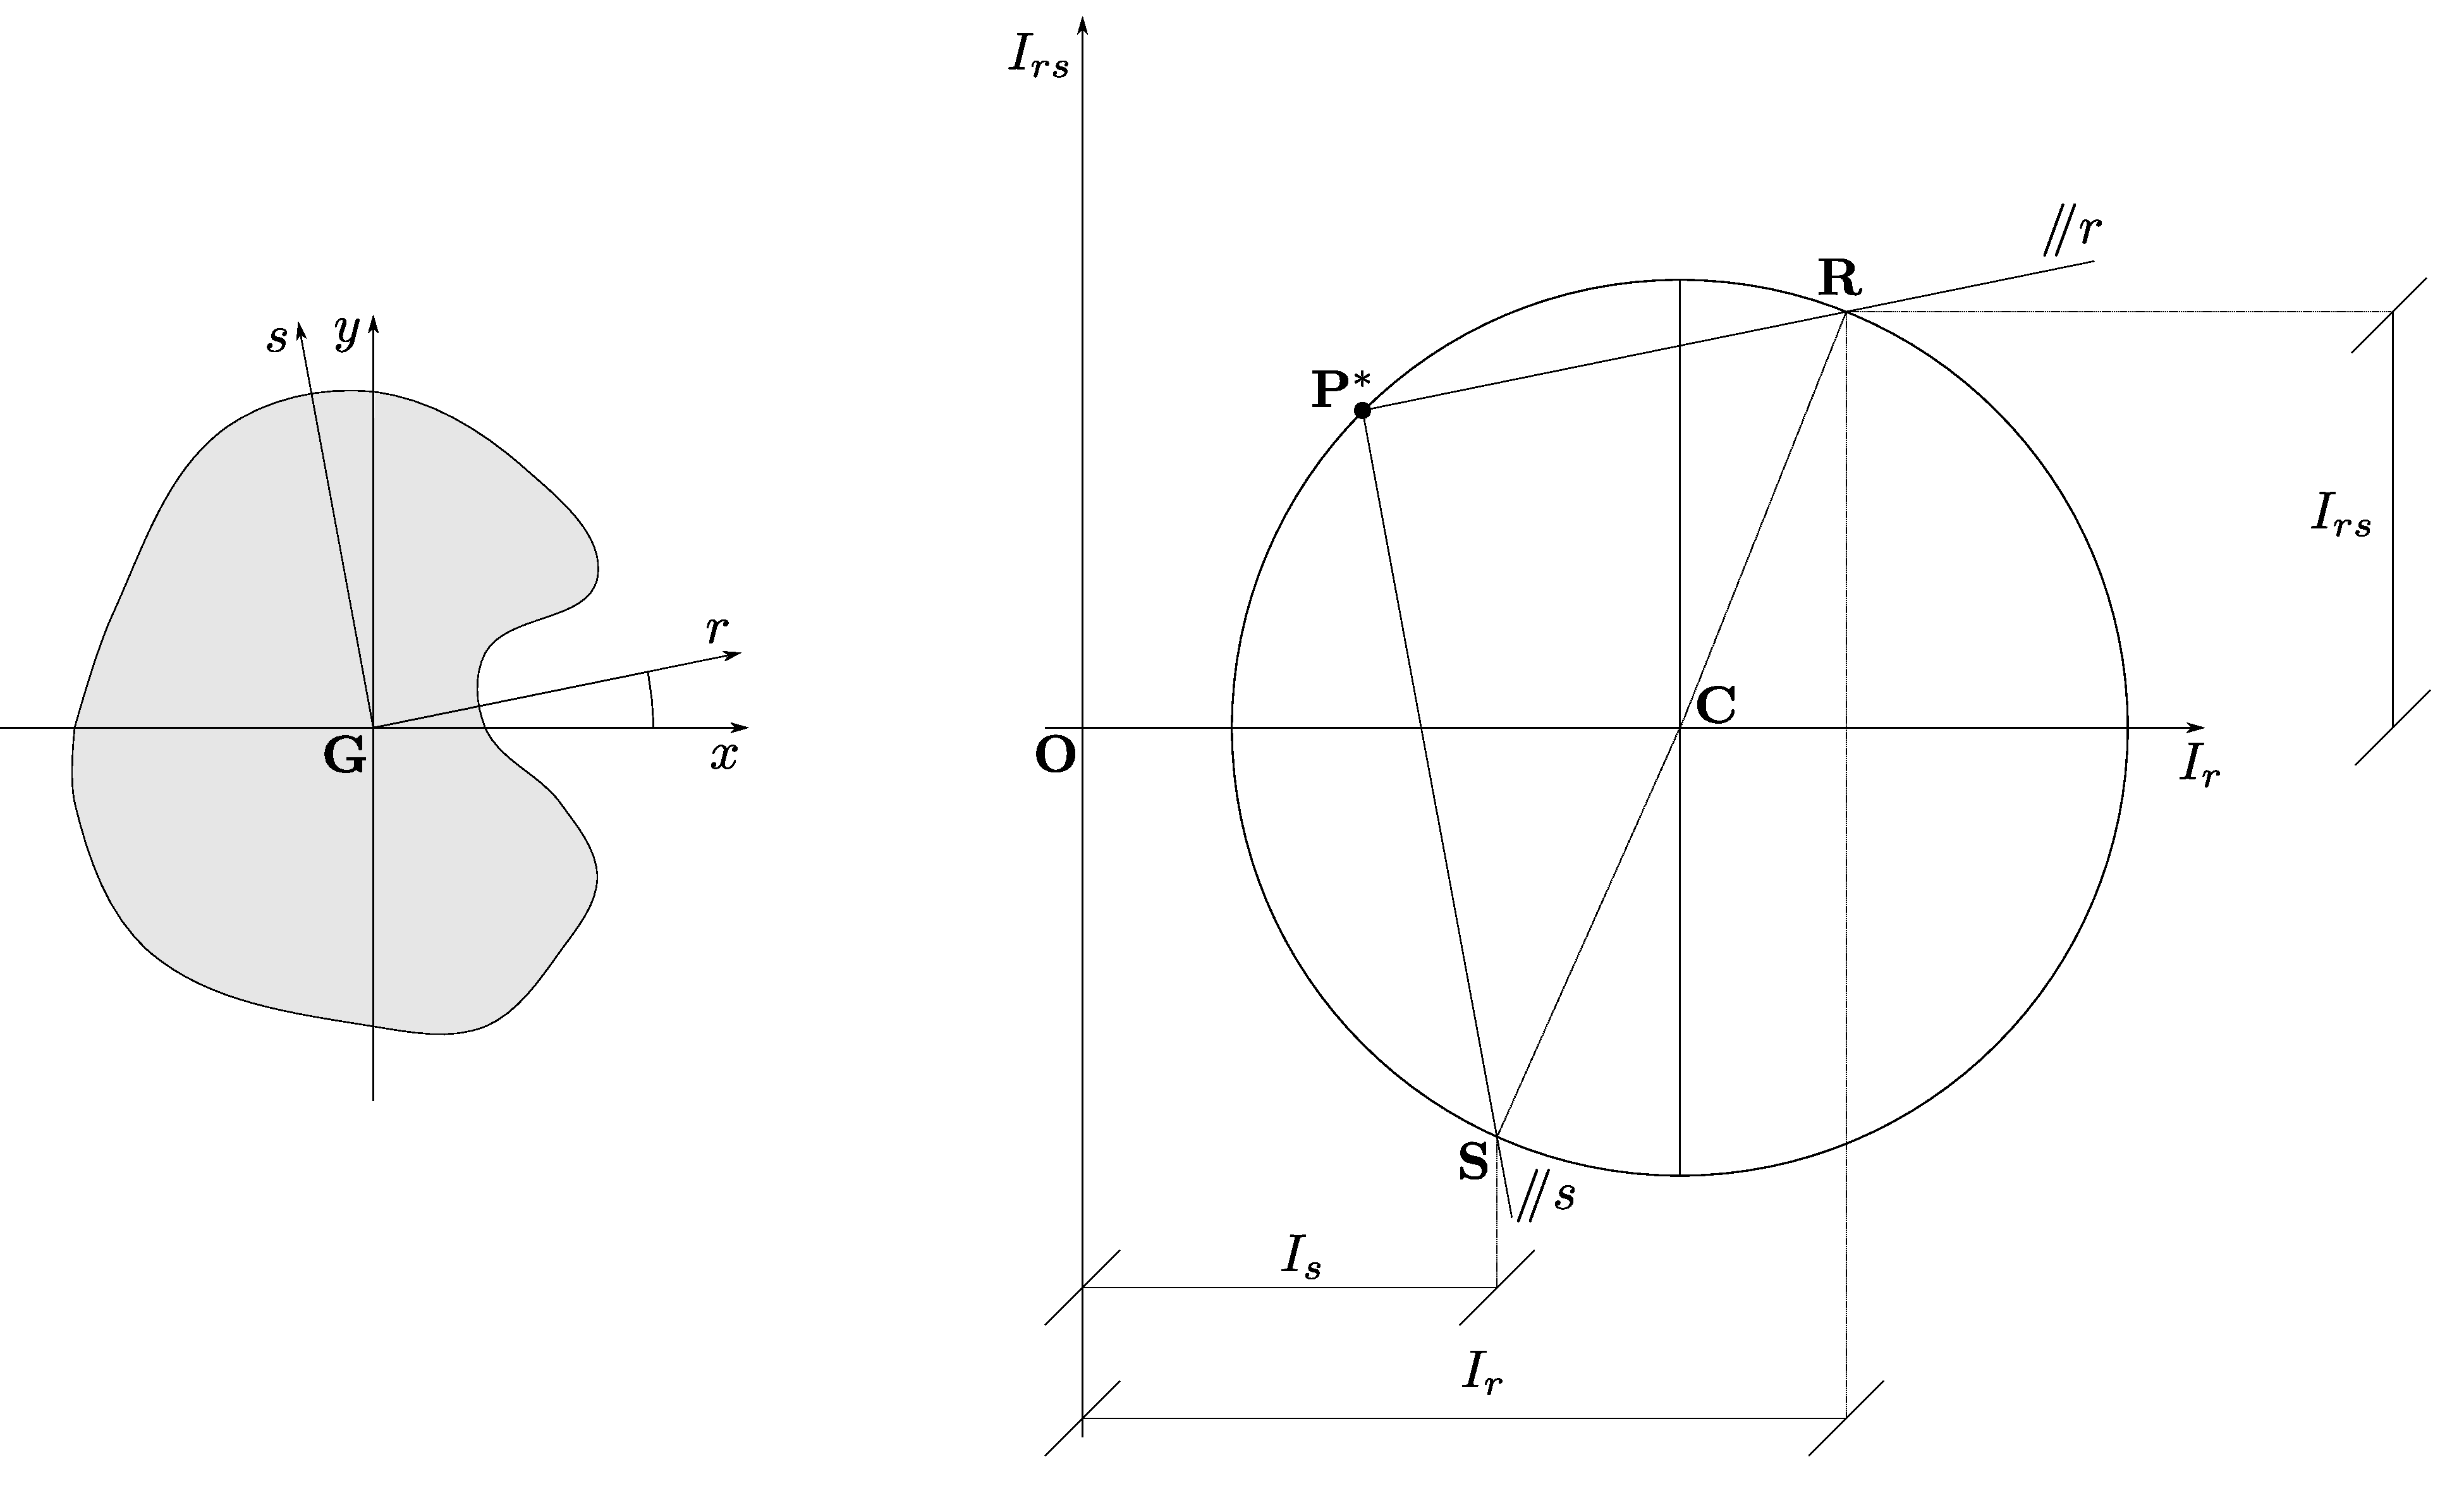
\includegraphics[width=\textwidth]{Immagini/Parte_5/Figura5_2/Figura5_2.pdf}
\caption{}
\label{figura5-2}
\end{figure}
%----------------------------------------------------------------------------------------
\noindent Con l'ausilio della figura~\ref{figura5-2}, cercheremo ora di capire come si utilizza il cerchio di Mohr. Siano $r$ ed $s$ due rette baricentriche, ortogonali, orientate in modo che la coppia $rs$ sia sovrapponibile alla coppia $xy$. 

\noindent Le formule~\eqref{equazione4-1} consentono, noti $I_x$, $I_y$ ed $I_{xy}$ di calcolare $I_r$, $I_s$ ed $I_{rs}$ identificando con $r$ l'asse $x'$ e con $s$ l'asse $y'$; ma noi, in questo paragrafo, vedremo come è possibile ottenere i valori di $I_r$, $I_s$ ed $I_{rs}$ grazie al cerchio di Mohr.
%--------------------------------------------------------------------------------------------------------------------------------------------------------------

\noindent Si tracciano per $\mathbf{P}^{*}$ le parallele ad $r$ e ad $s$; esse intersecano la circonferenza rispettivamente nei punti $\mathbf{R}$ ed $\mathbf{S}$; essendo le rette $r$ ed $s$ ortogonali, consegue che i punti $\mathbf{R}$ ed $\mathbf{S}$ sono \textsc{diametralmente opposti}. Ebbene, in forza della~\eqref{equazione4-1}, si potrebbe dimostrare che
%--------------------------------------------------------------------------------------------------------------------------------------------------------------
\begin{align*}
\textup{\textsc{Ascissa di }}\mathbf{R} &= I_r \\
\textup{\textsc{Ascissa di }}\mathbf{S} &= I_s \\
\textup{\textsc{Ordinata di }}\mathbf{R} &= I_{rs} 
\end{align*}
%--------------------------------------------------------------------------------------------------------------------------------------------------------------
%----------------------------------------------------------------------------------------
\renewcommand{\thefigure}{5~-~3}
\begin{figure}[ht]
\centering
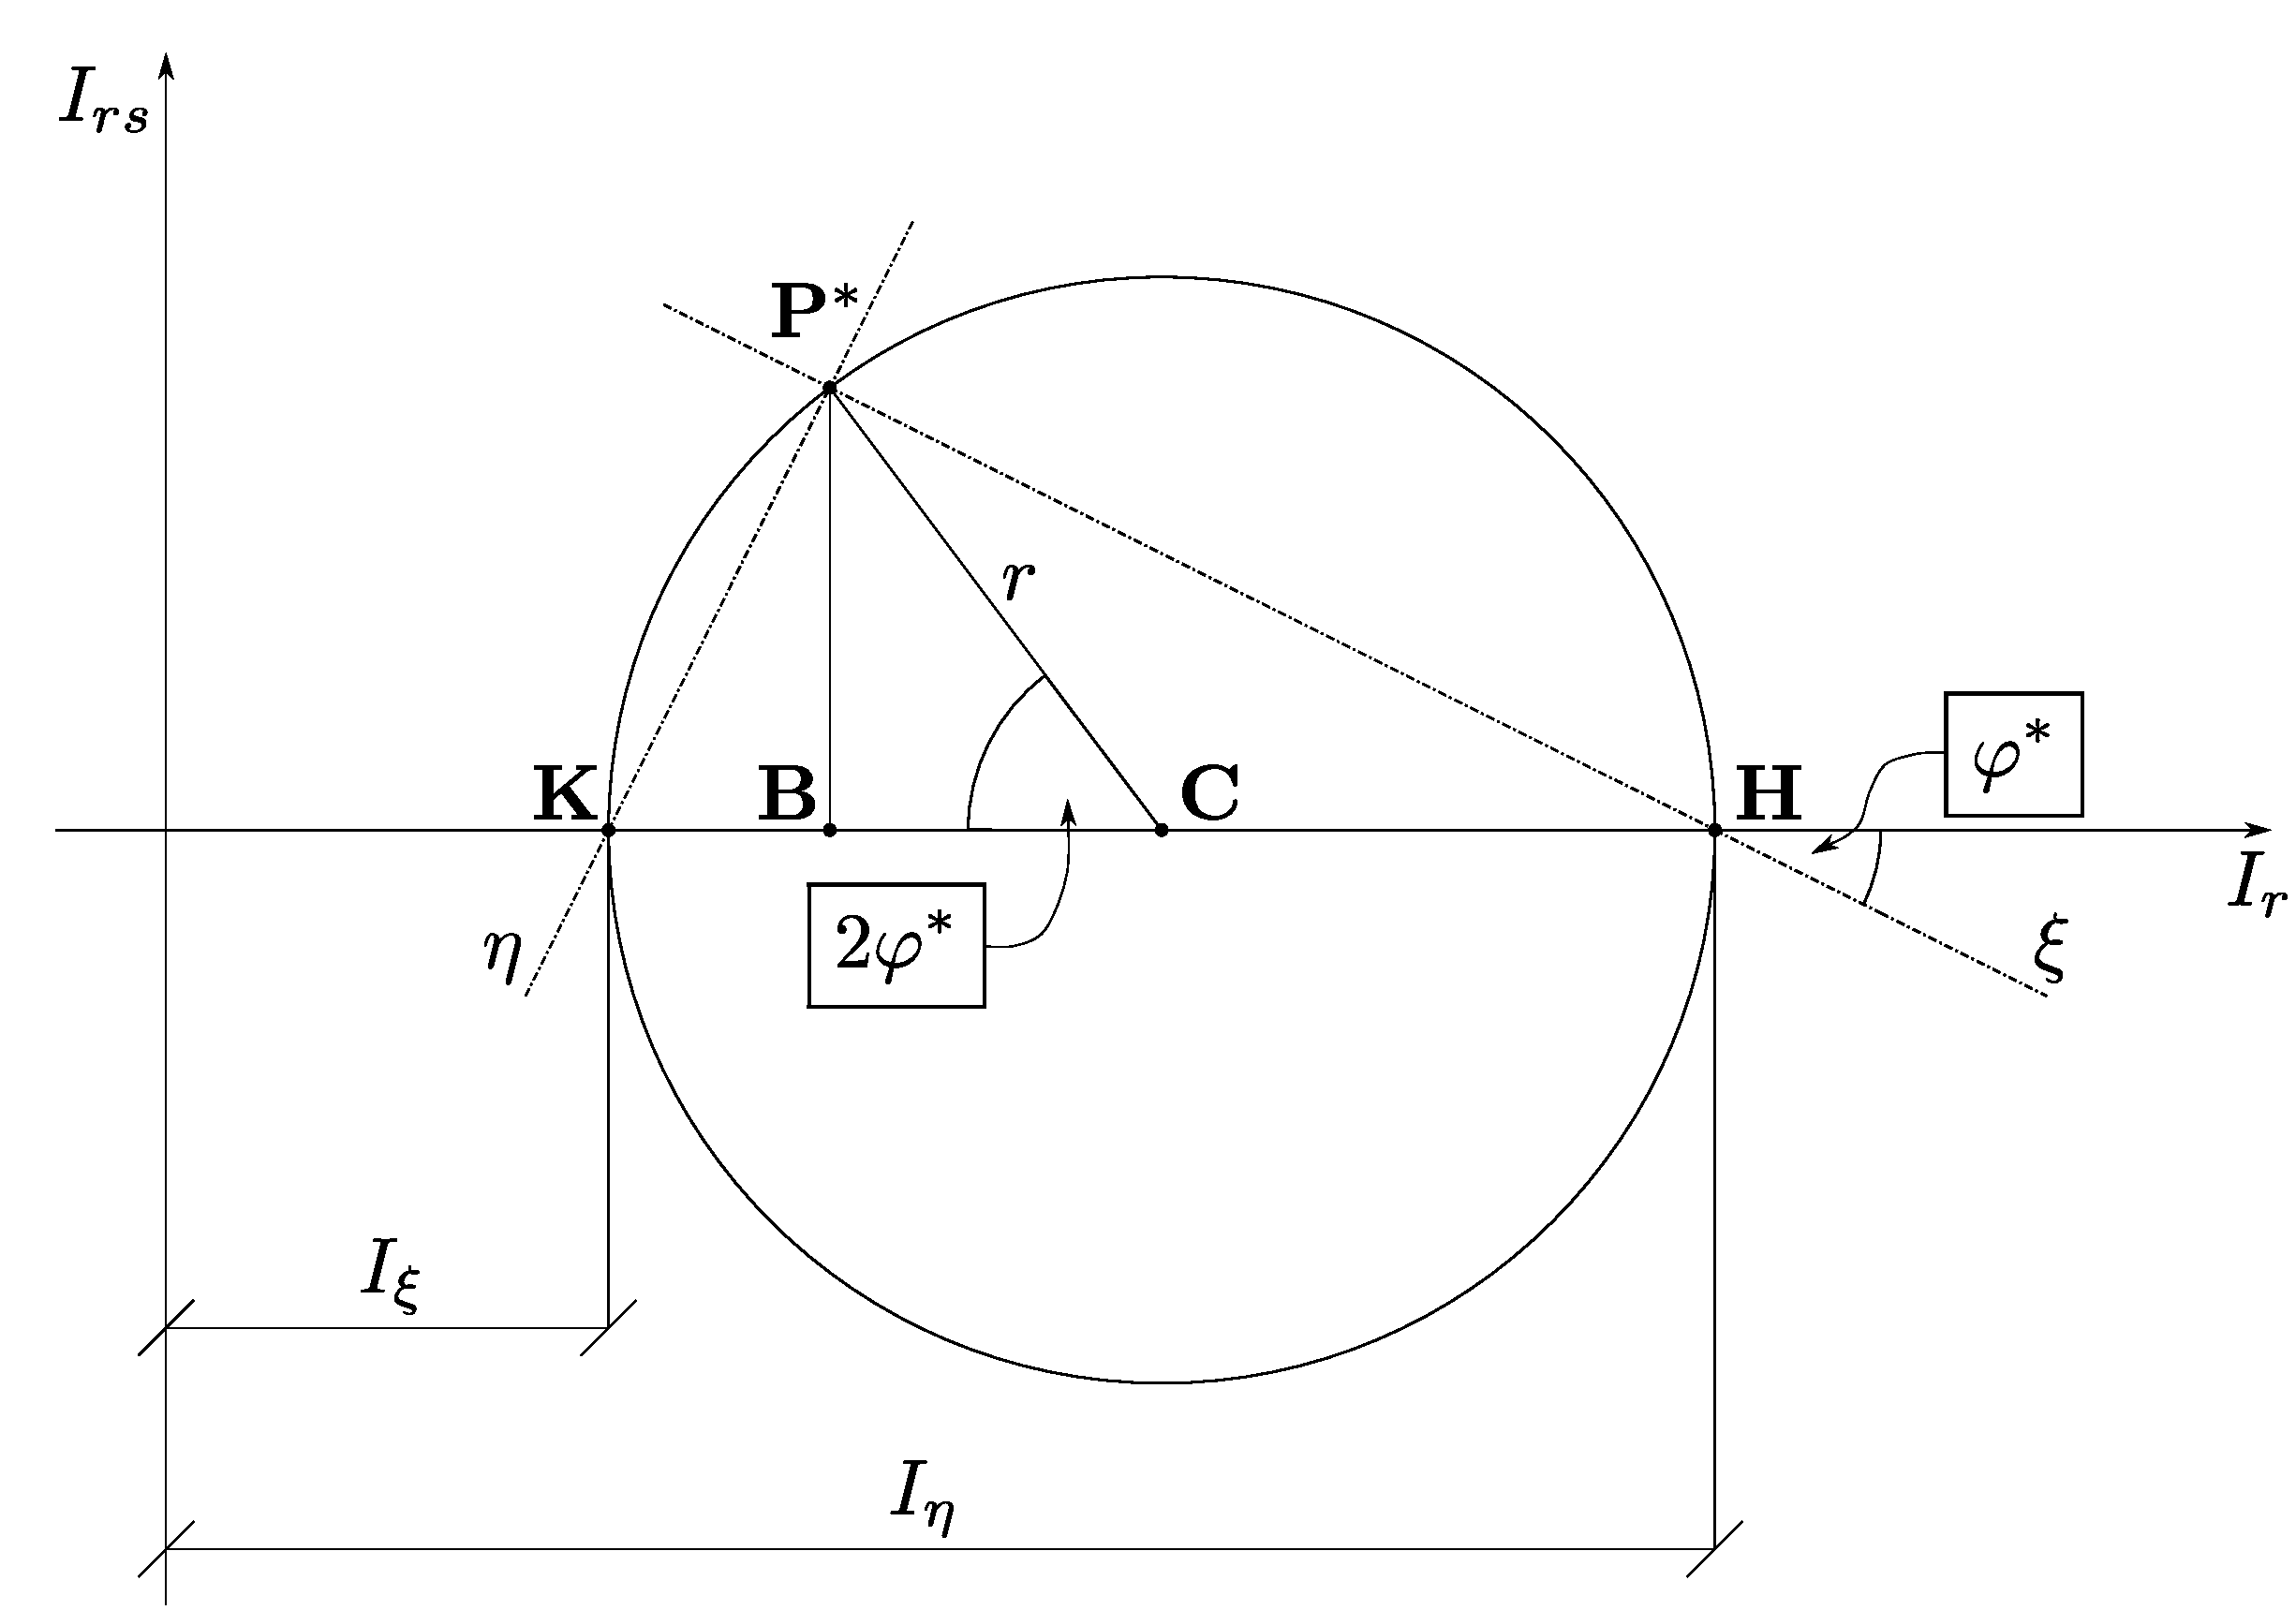
\includegraphics[width=\textwidth]{Immagini/Parte_5/Figura5_3/Figura5_3.pdf}
\caption{}
\label{figura5-3}
\end{figure}
%----------------------------------------------------------------------------------------
Facciamo ora riferimento alla figura~\ref{figura5-3}: qui sono evidenziati i punti $\mathbf{H}$ e $\mathbf{K}$, estremi del diametro orizzontale. Le rette che congiungono $\mathbf{P}^{*}$ con $\mathbf{H}$ e $\mathbf{K}$ sono evidentemente caratterizzate dai seguenti requisiti:
%--------------------------------------------------------------------------------------------------------------------------------------------------------------
\begin{enumerate}
\item sono ortogonali
\item è nullo il momento centrifugo rispetto ad esse, essendo nulle le ordinate dei punti $\mathbf{H}$ e $\mathbf{K}$
\item i momenti di inerzia rispetto ad esse sono uno \textsc{massimo} e l'altro \textsc{minimo}, tali essendo le ascisse dei punti $\mathbf{H}$ e $\mathbf{K}$
\end{enumerate}
%--------------------------------------------------------------------------------------------------------------------------------------------------------------
Si riconosce, così, che le rette in questione sono gli assi principali di inerzia.
%--------------------------------------------------------------------------------------------------------------------------------------------------------------
È bene sottolineare che l'asse $\xi$ coinciderà con quella, delle due rette $\mathbf{P}^{*}\mathbf{H}$ e $\mathbf{P}^{*}\mathbf{P}$, che forma con l'asse $I_r$ l'angolo \textsc{minore}. Il valore $\varphi^{*}=\widehat{\xi x}$ si può dedurre agevolmente dalla figura~\ref{figura5-3}. Con semplici considerazioni geometriche si trova che:
%--------------------------------------------------------------------------------------------------------------------------------------------------------------
\begin{equation*}
\tan 2\varphi^{*} = -\frac{\lvert \,\mathbf{B}\mathbf{P}^{*} \,\lvert}{\lvert \,\mathbf{B}\mathbf{C} \,\lvert}
\end{equation*}
%--------------------------------------------------------------------------------------------------------------------------------------------------------------
Il segno meno si giustifica alla luce del fatto che, in figura~\ref{figura5-3}, $\varphi^{*}$ risulta essere negativo perché orario. E poiché
%--------------------------------------------------------------------------------------------------------------------------------------------------------------
\begin{align*}
\lvert \, \mathbf{B}\mathbf{P}^{*}\,\lvert &= I_{xy} \\ 
\lvert \, \mathbf{B}\mathbf{C}\,\lvert &= \frac{I_{x}-I_{y}}{2} 
\end{align*}
%--------------------------------------------------------------------------------------------------------------------------------------------------------------
si trova
%--------------------------------------------------------------------------------------------------------------------------------------------------------------
\begin{equation*}
\tan 2\varphi^{*} = -\frac{2I_{xy}}{I_{x}-I_{y}}
\end{equation*}
%--------------------------------------------------------------------------------------------------------------------------------------------------------------
relazione che, riconosciamo, essere coincidente con la~\eqref{equazione4-2} qui ritrovata attraverso il cerchio di Mohr.
%--------------------------------------------------------------------------------------------------------------------------------------------------------------

\noindent Dalla figura~\ref{figura5-3} appare inoltre evidente che 
%--------------------------------------------------------------------------------------------------------------------------------------------------------------
\begin{align*}
I_{\xi} &= \lvert \, \mathbf{O}\mathbf{H} \, \lvert = \lvert \, \mathbf{O}\mathbf{C} \, \lvert + r \\
I_{\eta} &= \lvert \, \mathbf{O}\mathbf{K} \, \lvert = \lvert \, \mathbf{O}\mathbf{C} \, \lvert - r 
\end{align*}
%--------------------------------------------------------------------------------------------------------------------------------------------------------------
e cioè, per quanto si è visto dalla~\eqref{equazione5-1}
%--------------------------------------------------------------------------------------------------------------------------------------------------------------
\begin{equation*}
\begin{aligned}
I_{\xi} & \\
I_{\eta} &
\end{aligned}
\,\,\Biggr\}\,\, \frac{I_{x}+I_{y}}{2} \pm \sqrt{\biggl(\frac{I_{x}-I_{y}}{2}\biggr)^{2}+I_{xy}^{2}}
\end{equation*}
%--------------------------------------------------------------------------------------------------------------------------------------------------------------
La precedente formula è, forse, lo strumento più efficace per calcolare $I_{\xi}$ ed $I_{\eta}$; l'alternativa, come sappiamo, è utilizzare le prime due delle~\eqref{equazione4-1} ponendo in esse $\varphi^{*}$ in luogo di $\varphi$; tuttavia è opportuna una precisazione: in essa compare il simbolo $\pm$ dove il $+$ è riferito ad $I_{\xi}$ ed il $-$ ad $I_{\eta}$; ebbene ciò è vero se 
%--------------------------------------------------------------------------------------------------------------------------------------------------------------
\begin{equation*}
\boxed{I_{x} > I_{y}}
\end{equation*}
%--------------------------------------------------------------------------------------------------------------------------------------------------------------
Se invece $I_{x}<I_{y}$, bisognerà porre $\mp$ in essa. In definitiva 
%--------------------------------------------------------------------------------------------------------------------------------------------------------------
\begin{align}
\boxed{\textup{\textsc{se }}I_{x} > I_{y}} &\longrightarrow \boxed{\frac{I_{x}+I_{y}}{2} \pm \sqrt{\biggl(\frac{I_{x}-I_{y}}{2}\biggr)^{2}+I_{xy}^{2}}}\tag{5.2a} \label{equazione5-2a} \\
\boxed{\textup{\textsc{se }}I_{x} < I_{y}} &\longrightarrow \boxed{\frac{I_{x}+I_{y}}{2} \mp \sqrt{\biggl(\frac{I_{x}-I_{y}}{2}\biggr)^{2}+I_{xy}^{2}}} \tag{5.2b} \label{equazione5-2b}
\end{align}
%--------------------------------------------------------------------------------------------------------------------------------------------------------------
\clearpage
\section{Esercizi}
\paragraph{Esercizio 5.1}

\noindent Con riferimento al profilato dell'Esercizio 4.1, si richiede
\begin{enumerate}
\item di costruire il cerchio di Mohr;
\item di calcolare $I_{\xi}$ ed $I_{\eta}$ utilizzando le relazioni~\eqref{equazione5-2a} e~\eqref{equazione5-2b};
\item di individuare la coppia di rette, ortogonali e baricentriche, rispetto a cui è massimo il momento centrifugo e trovarne il valore;
\item di trovare il valore dei momenti di inerzia di cui in 3;
\item di determinare sia graficamente che analiticamente, i valori di $I_r$, $I_s$ ed $I_{rs}$, essendo $r$ la retta che forma con $x$ l'angolo di $45^{\circ}$.
\end{enumerate}
%--------------------------------------------------------------------------------------------------------------------------------------------------------------

\noindent \subparagraph{Quesito 1}  Sappiamo già che (si riveda l'Esercizio 4.1)
%--------------------------------------------------------------------------------------------------------------------------------------------------------------
\begin{align*}
I_x &= 16155\,\textup{cm}^{4} \\
I_y &= 7675\,\textup{cm}^{4} \\
I_{xy} &= -7966\,\textup{cm}^{4}
\end{align*}
%--------------------------------------------------------------------------------------------------------------------------------------------------------------
I connotati del cerchio di Mohr del profilato in questione, sono, dunque:
%--------------------------------------------------------------------------------------------------------------------------------------------------------------
\begin{align*}
\lvert \, \mathbf{O}\mathbf{C}\,\lvert &= \frac{I_{x}+I_{y}}{2} = 11915\,\textup{cm}^{4} \\
r &= \sqrt{\biggl(\frac{I_{x}-I_{y}}{2}\biggr)^{2}+I_{xy}^{2}} = 9024\,\textup{cm}^{4}
\end{align*}
%--------------------------------------------------------------------------------------------------------------------------------------------------------------
Alla luce di questi connotati, andiamo a stabilire la \textsc{scala} con cui trasformeremo in $\textup{cm}$ i momenti del secondo ordine. Se vogliamo che il cerchio entri in un foglio come questo, con formato \textsc{a}$4$, dobbiamo far sì che il suo raggio sia nettamente minore di $10\,\textup{cm}$. Assumendo la \textsc{scala momenti del secondo ordine} pari a
%--------------------------------------------------------------------------------------------------------------------------------------------------------------
\begin{equation*}
1\,\textup{cm} = 1500\,\textup{cm}^{4}
\end{equation*}
%--------------------------------------------------------------------------------------------------------------------------------------------------------------
avremo un raggio
%--------------------------------------------------------------------------------------------------------------------------------------------------------------
\begin{equation*}
r = \frac{9024}{1500} \approx 6\,\textup{cm}
\end{equation*}
%--------------------------------------------------------------------------------------------------------------------------------------------------------------
Le coordinate sul cerchio di Mohr del polo $\mathbf{P}^{*}$ sono, conseguentemente 
%--------------------------------------------------------------------------------------------------------------------------------------------------------------
\begin{equation*}
\mathbf{P}^{*}(I_y,\,I_{xy}) \rightarrow \mathbf{P}^{*}\biggl(\frac{7675}{1500},\,-\frac{7966}{1500}\biggr) \rightarrow \mathbf{P}^{*}(5.12\,\textup{cm},\,-5.31\,\textup{cm})
\end{equation*}
%--------------------------------------------------------------------------------------------------------------------------------------------------------------
Il lettore è invitato a controllare la coincidenza di questi risultati con quelli trovati alla fine dell'Esercizio 4.1.
%--------------------------------------------------------------------------------------------------------------------------------------------------------------
%----------------------------------------------------------------------------------------
\renewcommand{\thefigure}{5.1~-~1}
\begin{figure}[ht]
\centering
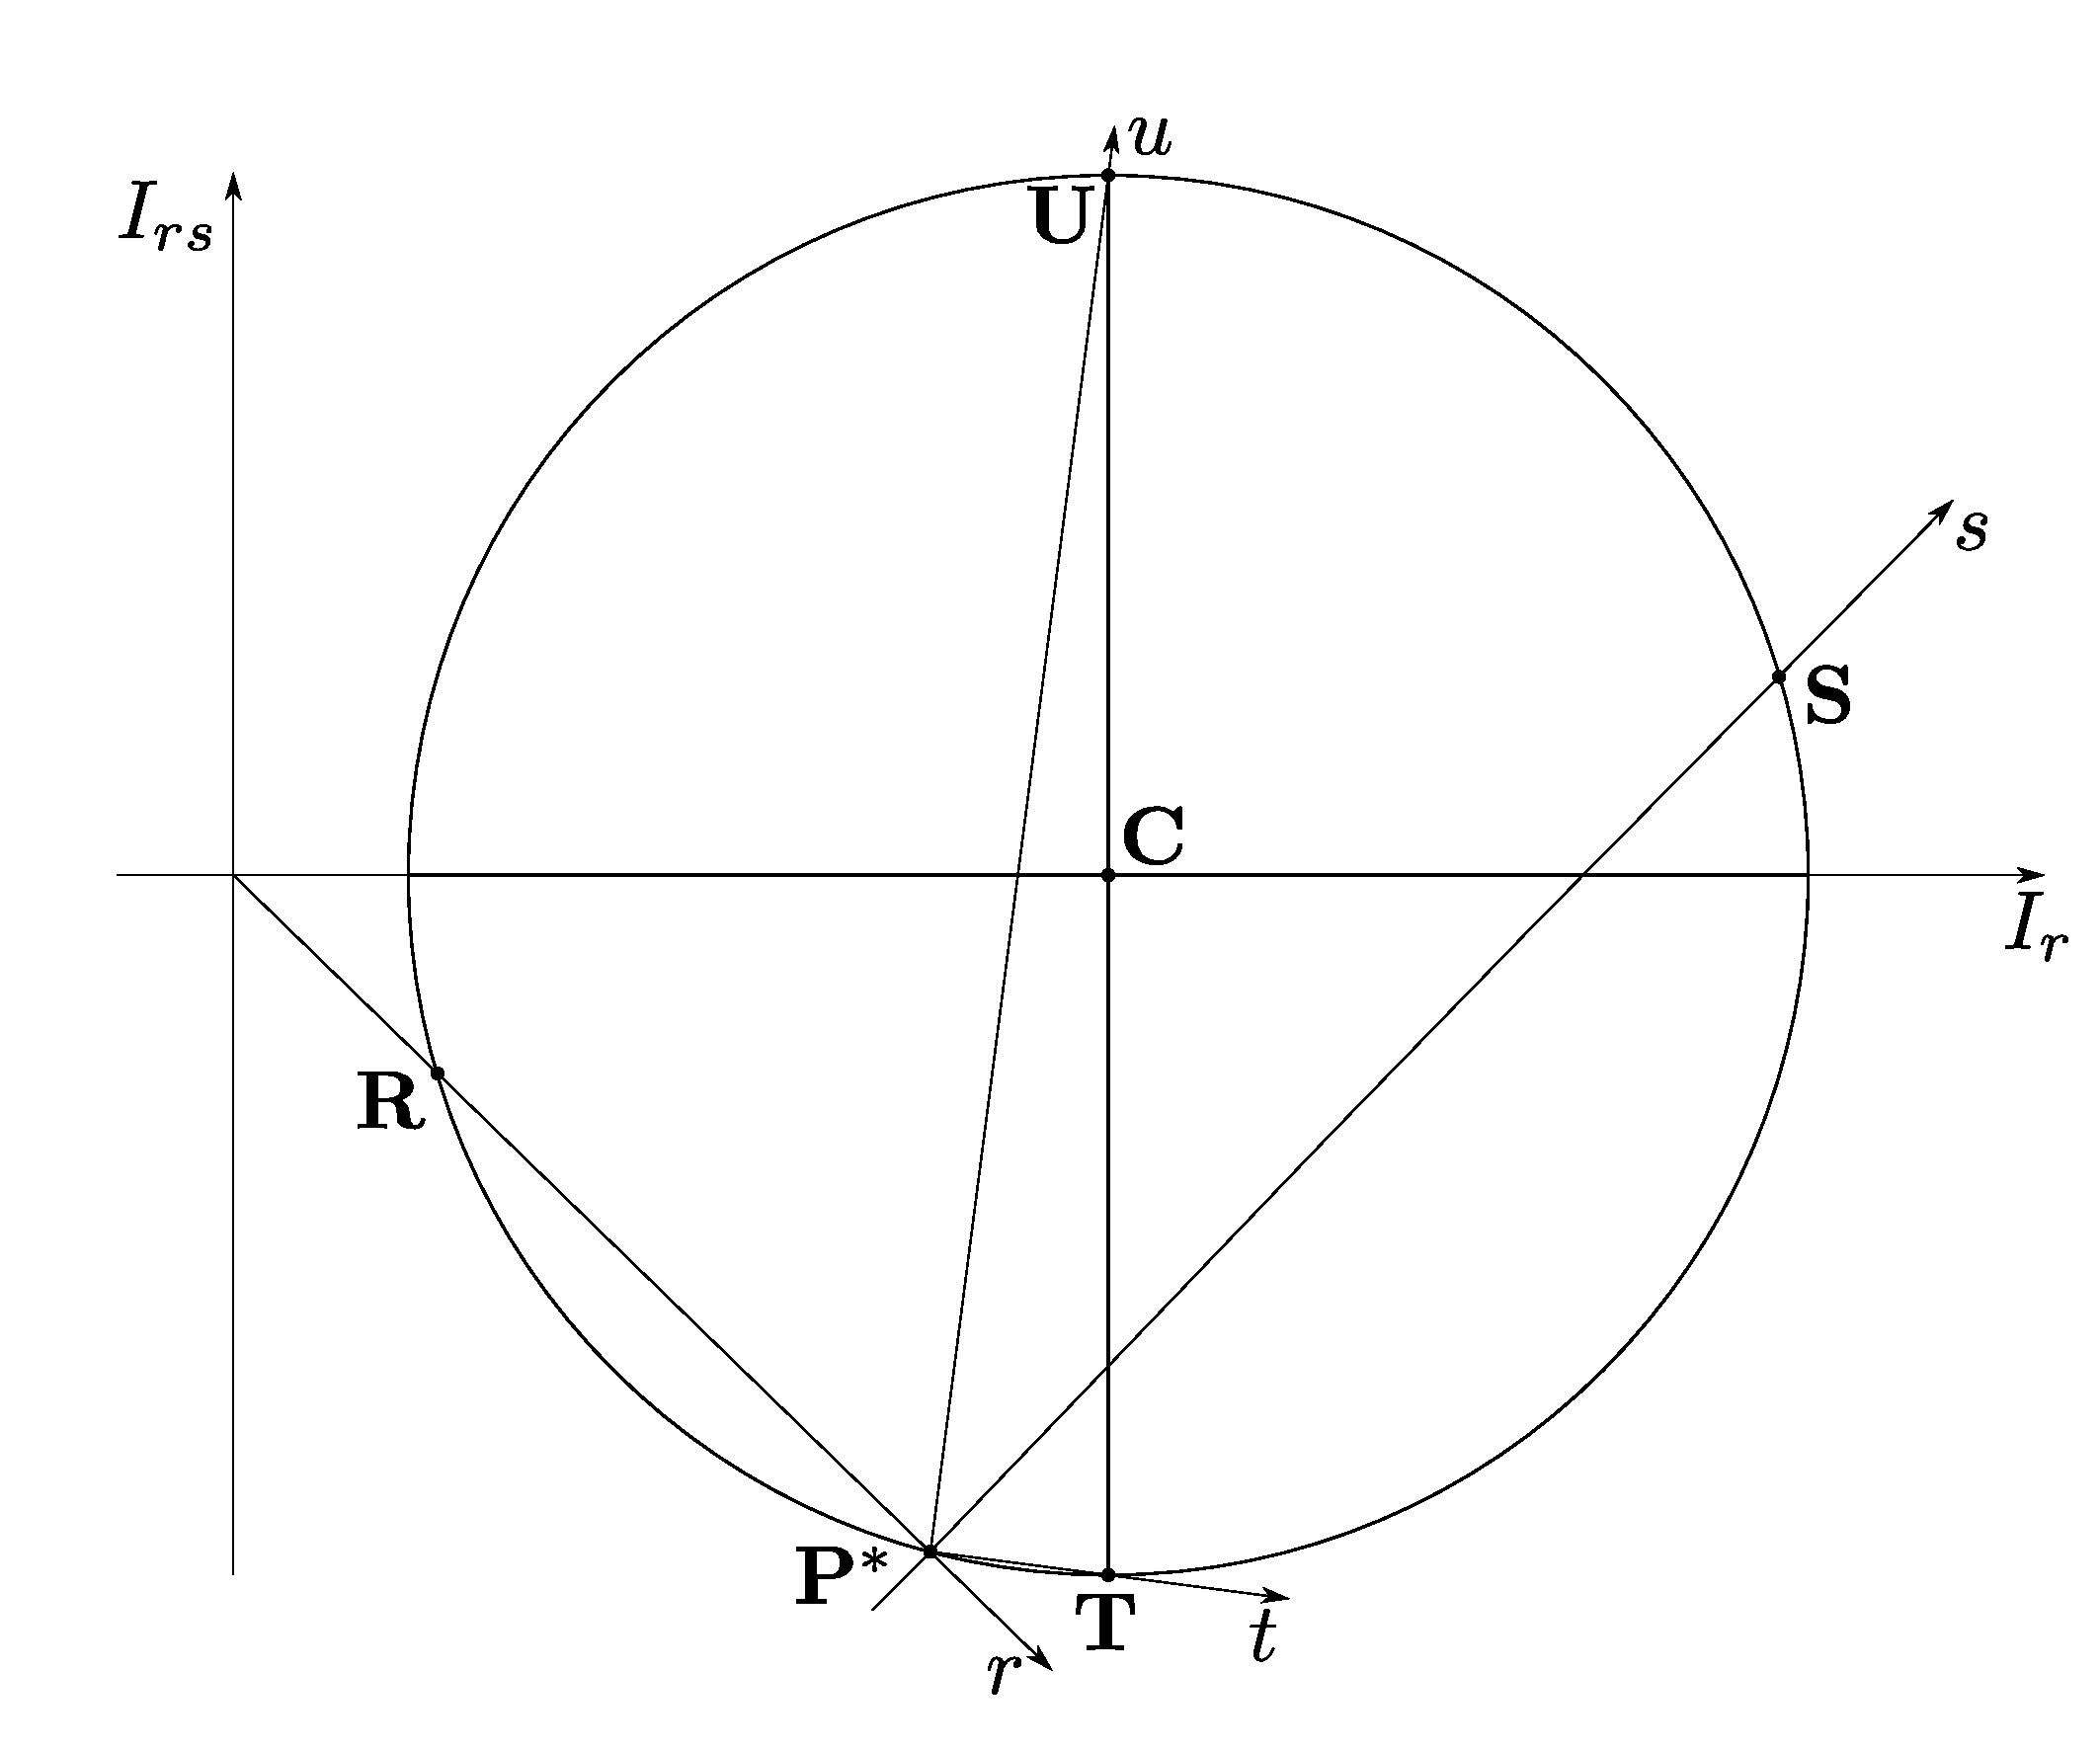
\includegraphics[width=\textwidth]{Immagini/Parte_5/Esercizio5_1/Esercizio5_1_1.pdf}
\caption{}
\label{Esercizio5-1-1}
\end{figure}
%----------------------------------------------------------------------------------------
\noindent \subparagraph{Quesito 3} La coppia di rette rispetto alle quali è massimo il momento centrifugo è, ovviamente, quella che si ottiene congiungendo il polo $\mathbf{P}^{*}$ con i punti $\mathbf{T}$ ed $\mathbf{U}$ estremi del diametro verticale. Orientate le rette $\mathbf{P}^{*}\mathbf{T}=t$ e $\mathbf{P}^{*}\mathbf{U}=u$ come in figura, chiaramente risulta:
%--------------------------------------------------------------------------------------------------------------------------------------------------------------
\begin{equation*}
I_{tu} = \textup{\textsc{ordinata di }}\mathbf{T} = -r = -9024\,\textup{cm}^{4}
\end{equation*}
%--------------------------------------------------------------------------------------------------------------------------------------------------------------
\noindent \subparagraph{Quesito 4} Chiaramente 
%--------------------------------------------------------------------------------------------------------------------------------------------------------------
\begin{equation*}
I_t = I_u = \lvert\, \mathbf{O}\mathbf{C}\,\lvert = 11915\,\textup{cm}^{4}
\end{equation*}
%--------------------------------------------------------------------------------------------------------------------------------------------------------------
\noindent \subparagraph{Quesito 5} La retta $r$ e la sua normale $s$ si sono disegnate sempre sul cerchio in figura; esse si sono orientate così che la coppia $rs$ sia sovrapponibile alla coppia $xy$; abbiamo indicato, naturalmente, con $\mathbf{R}$ ed $\mathbf{S}$ le rispettive intersezioni di $r$ ed $s$ con la circonferenza. E, dunque, dal disegno si rileva
%--------------------------------------------------------------------------------------------------------------------------------------------------------------
\begin{align*}
I_r &= \textup{\textsc{ascissa di }} \mathbf{R} \cong 2.60\,\textup{cm} \longrightarrow 3900\,\textup{cm}^{4} \\
I_s &= \textup{\textsc{ascissa di }} \mathbf{S} \cong 13.25\,\textup{cm} \longrightarrow 19875\,\textup{cm}^{4} \\
I_{rs} &= \textup{\textsc{ordinata di }}\mathbf{R} \cong -2.80\,\textup{cm} \longrightarrow -4200\,\textup{cm}^{4}
\end{align*}
%--------------------------------------------------------------------------------------------------------------------------------------------------------------
Applicando le~\eqref{equazione4-1}, ponendo in esse $\varphi^{*}=45^{\circ}$, si trova che
%--------------------------------------------------------------------------------------------------------------------------------------------------------------
\begin{align*}
I_r &= 3949\,\textup{cm}^{4} \\
I_s &= 19881\,\textup{cm}^{4} \\
I_{rs} &= 4240\,\textup{cm}^{4} 
\end{align*}
%--------------------------------------------------------------------------------------------------------------------------------------------------------------
Naturalmente i valori \textsc{esatti} sono questi ultimi; lo scarto, peraltro molto modesto, è dovuto all'inevitabile errore nella misura delle distanze sul disegno in scala.
%--------------------------------------------------------------------------------------------------------------------------------------------------------------
%------------------------------------------------
\clearpage
\pagestyle{fancy}
\part{Ellisse centrale di inerzia}
\setcounter{section}{0}
\section{La definizione di raggio di inerzia}
%----------------------------------------------------------------------------------------
Si dice \textsc{raggio di inerzia} di una figura piana rispetto alla retta $r$ la distanza $\rho_r$ tale che 
%--------------------------------------------------------------------------------------------------------------------------------------------------------------
\begin{equation} \label{equazione6-1}
\boxed{I_r = A\rho_{r}^{2}}
\tag{6.1}
\end{equation}
%--------------------------------------------------------------------------------------------------------------------------------------------------------------
Ovviamente vale anche la seguente
%--------------------------------------------------------------------------------------------------------------------------------------------------------------
\begin{equation} \label{equazione6-1}
\boxed{\rho_r = \sqrt{\frac{I_r}{A}}}
\tag{6.2}
\end{equation}
%--------------------------------------------------------------------------------------------------------------------------------------------------------------
Se $r_0$ è la retta baricentrica parallela ad $r$ risulta, per il teorema del trasporto
%--------------------------------------------------------------------------------------------------------------------------------------------------------------
\begin{equation*}
I_r = I_{r_{0}} + Ad^2 \iff A\rho_{r}^{2} = A\rho_{r_{0}} + Ad^2
\end{equation*}
%--------------------------------------------------------------------------------------------------------------------------------------------------------------
e quindi
%--------------------------------------------------------------------------------------------------------------------------------------------------------------
\begin{equation*}
\rho_{r}^{2} = \rho_{r_{0}} + d^2
\end{equation*}
%--------------------------------------------------------------------------------------------------------------------------------------------------------------
Quest'ultima uguaglianza dimostra che $\rho_{r}>d$, che è la distanza di $\mathbf{G}$ da $r$; e da ciò segue la seguente proposizione
%--------------------------------------------------------------------------------------------------------------------------------------------------------------
\\

\fbox{\begin{minipage}{38em}
\centering
\textsc{Al fine di calcolare $I_r$ non è lecito pensare che l'area della figura sia concentrata in $\mathbf{G}$, il che si fa per calcolare il momento statico. Bisogna, eventualmente, concentrare l'area in un punto distante $\rho_r$ da $r$.}
\end{minipage}}
%--------------------------------------------------------------------------------------------------------------------------------------------------------------
\section{La definizione di ellisse centrale di inerzia}
%----------------------------------------------------------------------------------------
\renewcommand{\thefigure}{6~-~1}
\begin{figure}[h]
\centering
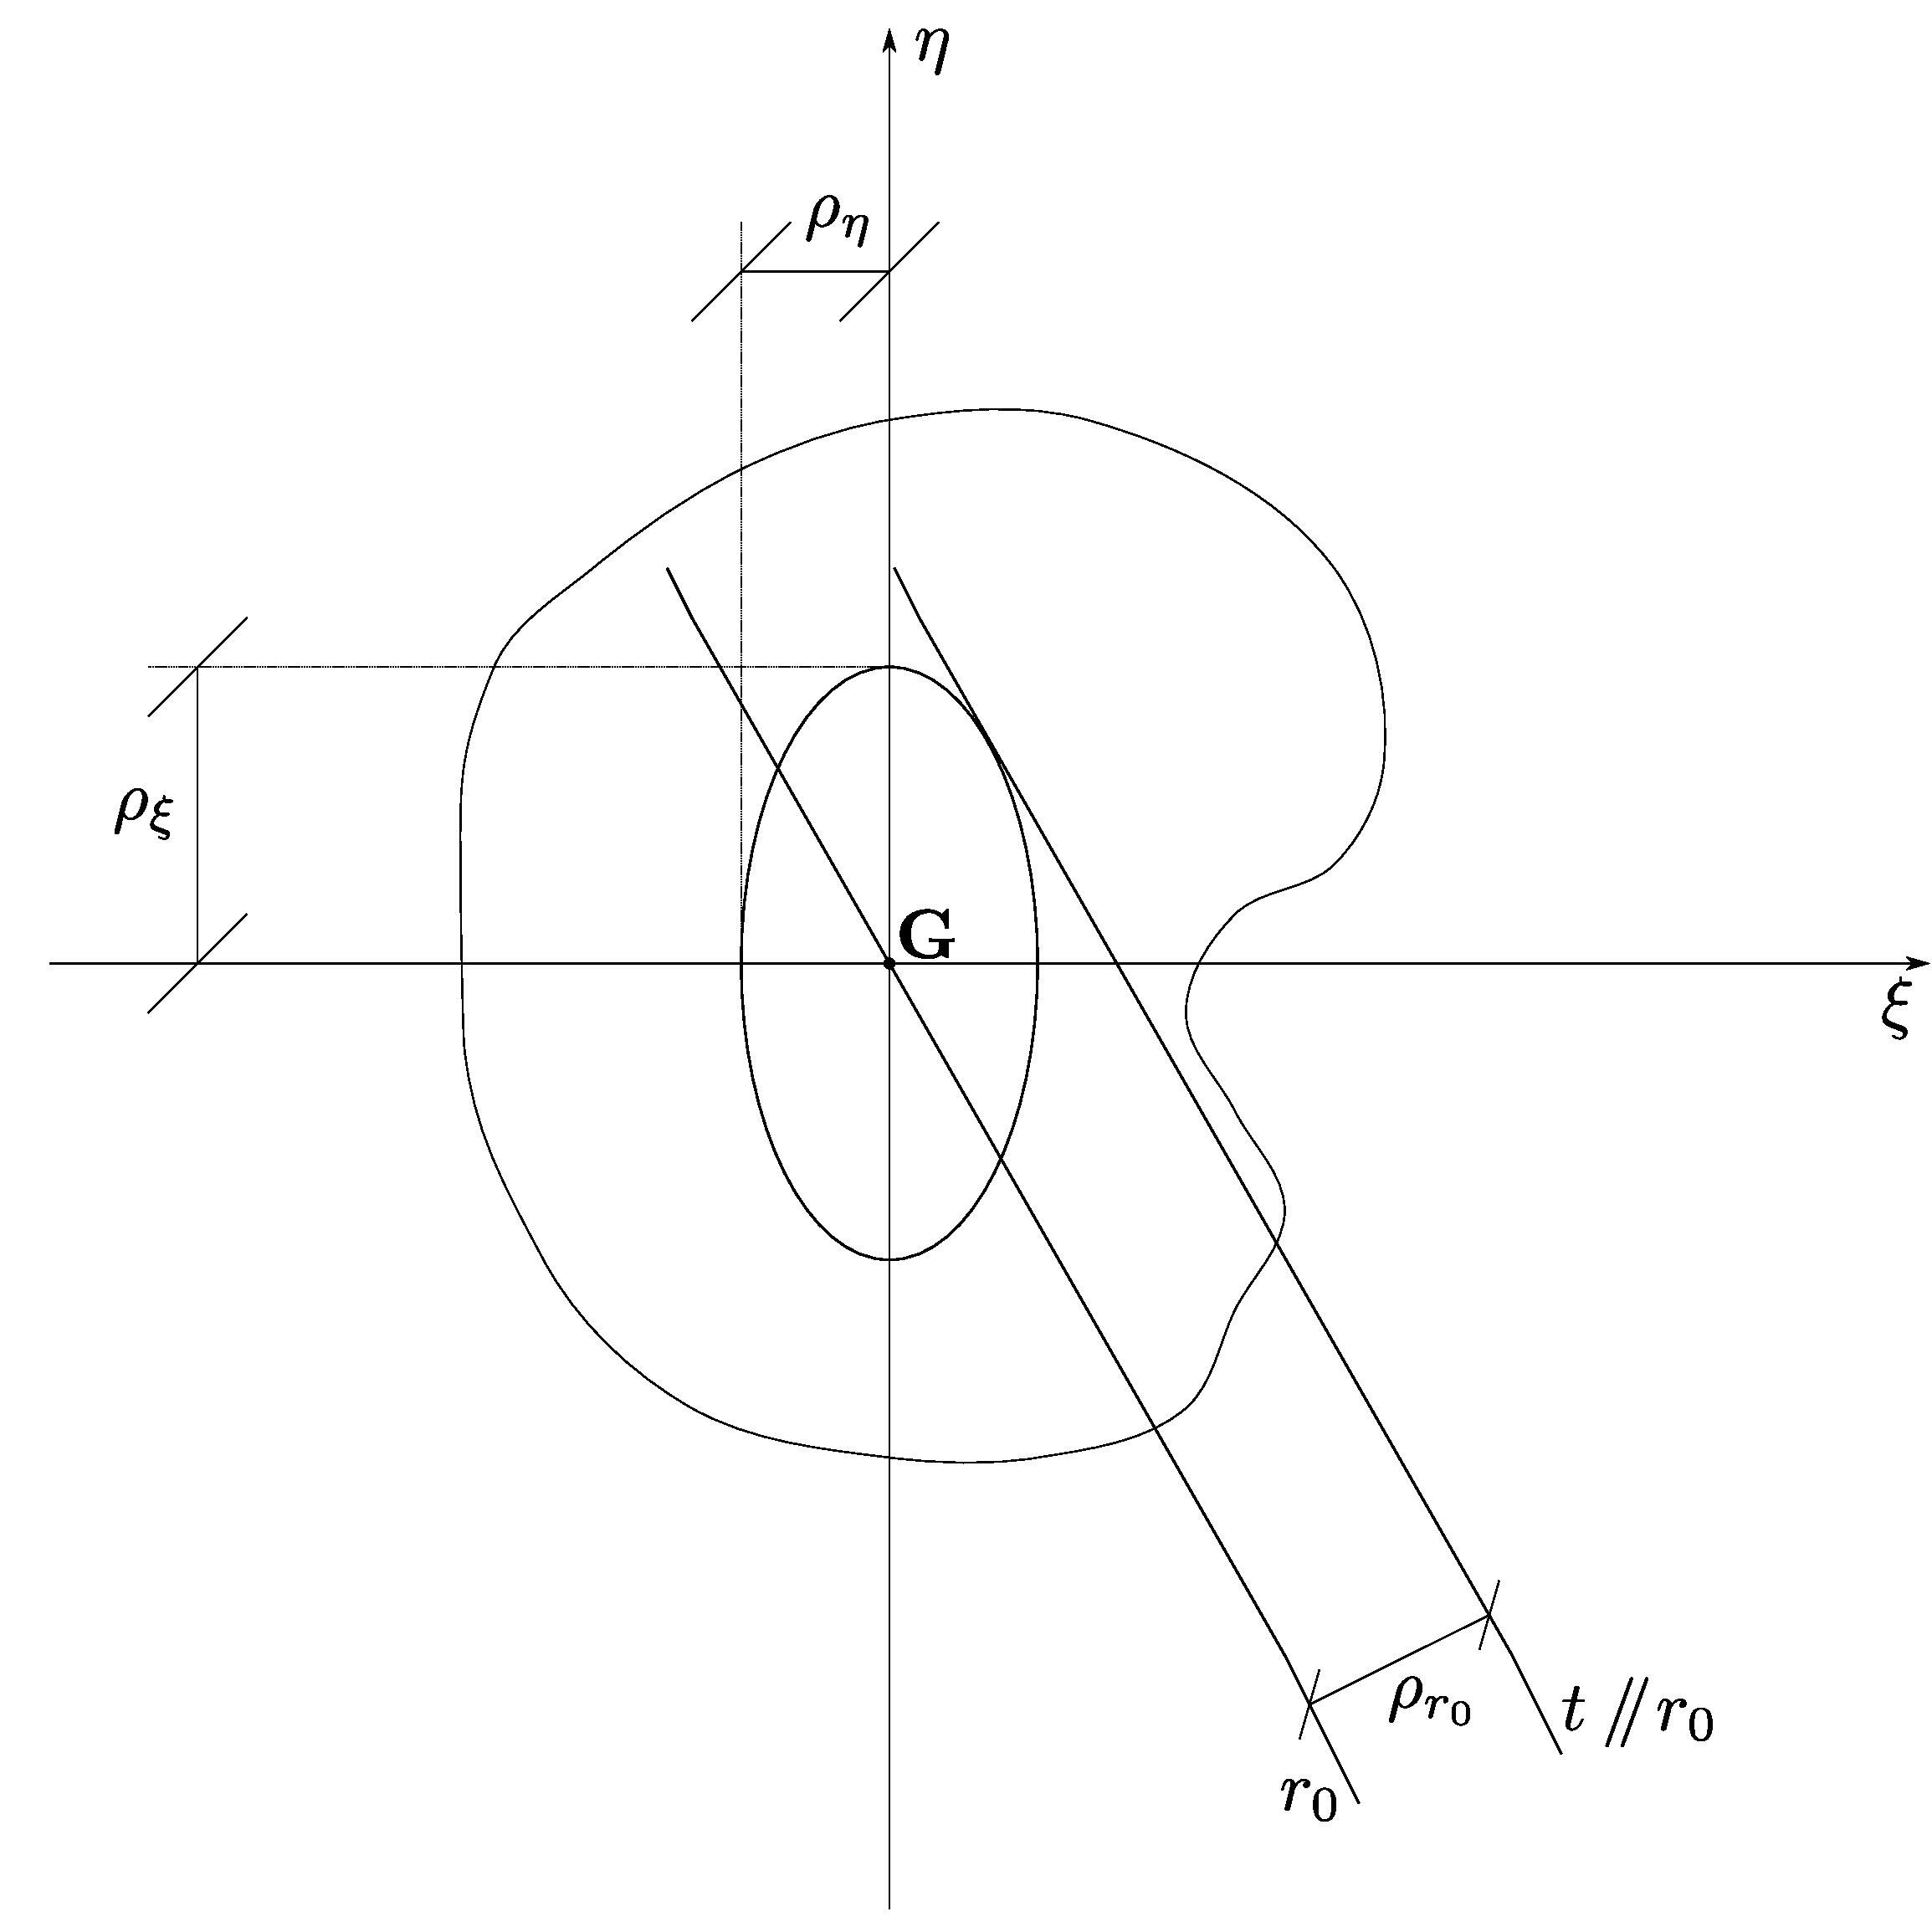
\includegraphics[width=0.75\textwidth]{Immagini/Parte_6/Figura6_1/Figura6_1.pdf}
\caption{}
\label{figura6-1}
\end{figure}
%--------------------------------------------------------------------------------------------------------------------------------------------------------------
Ogni figura piana ha la sua ellisse centrale di inerzia, si veda la figura~\ref{figura6-1}: si tratta dell'ellisse avente il centro coincidente con $\mathbf{G}$, gli assi di simmetria coincidenti con gli assi principali di inerzia $\xi$ ed $\eta$, i raggi principali di lunghezza $\rho_{\xi}$ e $\rho_{\eta}$; da notare che $\rho_{\eta}$ è disteso su $\xi$ e $\rho_{\xi}$ è disteso su $\eta$. In figura~\ref{figura6-1} è anche illustrata un'importante proprietà dell'ellisse di inerzia:
%--------------------------------------------------------------------------------------------------------------------------------------------------------------
\\

\fbox{\begin{minipage}{38em}
\centering
\textsc{Il raggio di inerzia di una figura rispetto ad una retta baricentrica $r_0$ è uguale alla distanza della stessa retta dalla sua parallela $t$ tangente all'ellisse.}
\end{minipage}}
\\
\\

%--------------------------------------------------------------------------------------------------------------------------------------------------------------
\noindent Come è noto dalla \textsc{geometria}, l'ellisse di~\ref{figura6-1} ha equazione
%--------------------------------------------------------------------------------------------------------------------------------------------------------------
\begin{equation} \label{equazione6-2}
\frac{\xi^2}{\rho_{\eta}^{2}}+\frac{\eta^2}{\rho_{\xi}^{2}} = 1
\tag{6.2}
\end{equation}
%--------------------------------------------------------------------------------------------------------------------------------------------------------------
\section{Diametri coniugati di un'ellisse}
%----------------------------------------------------------------------------------------
\renewcommand{\thefigure}{6~-~2}
\begin{figure}[h]
\centering
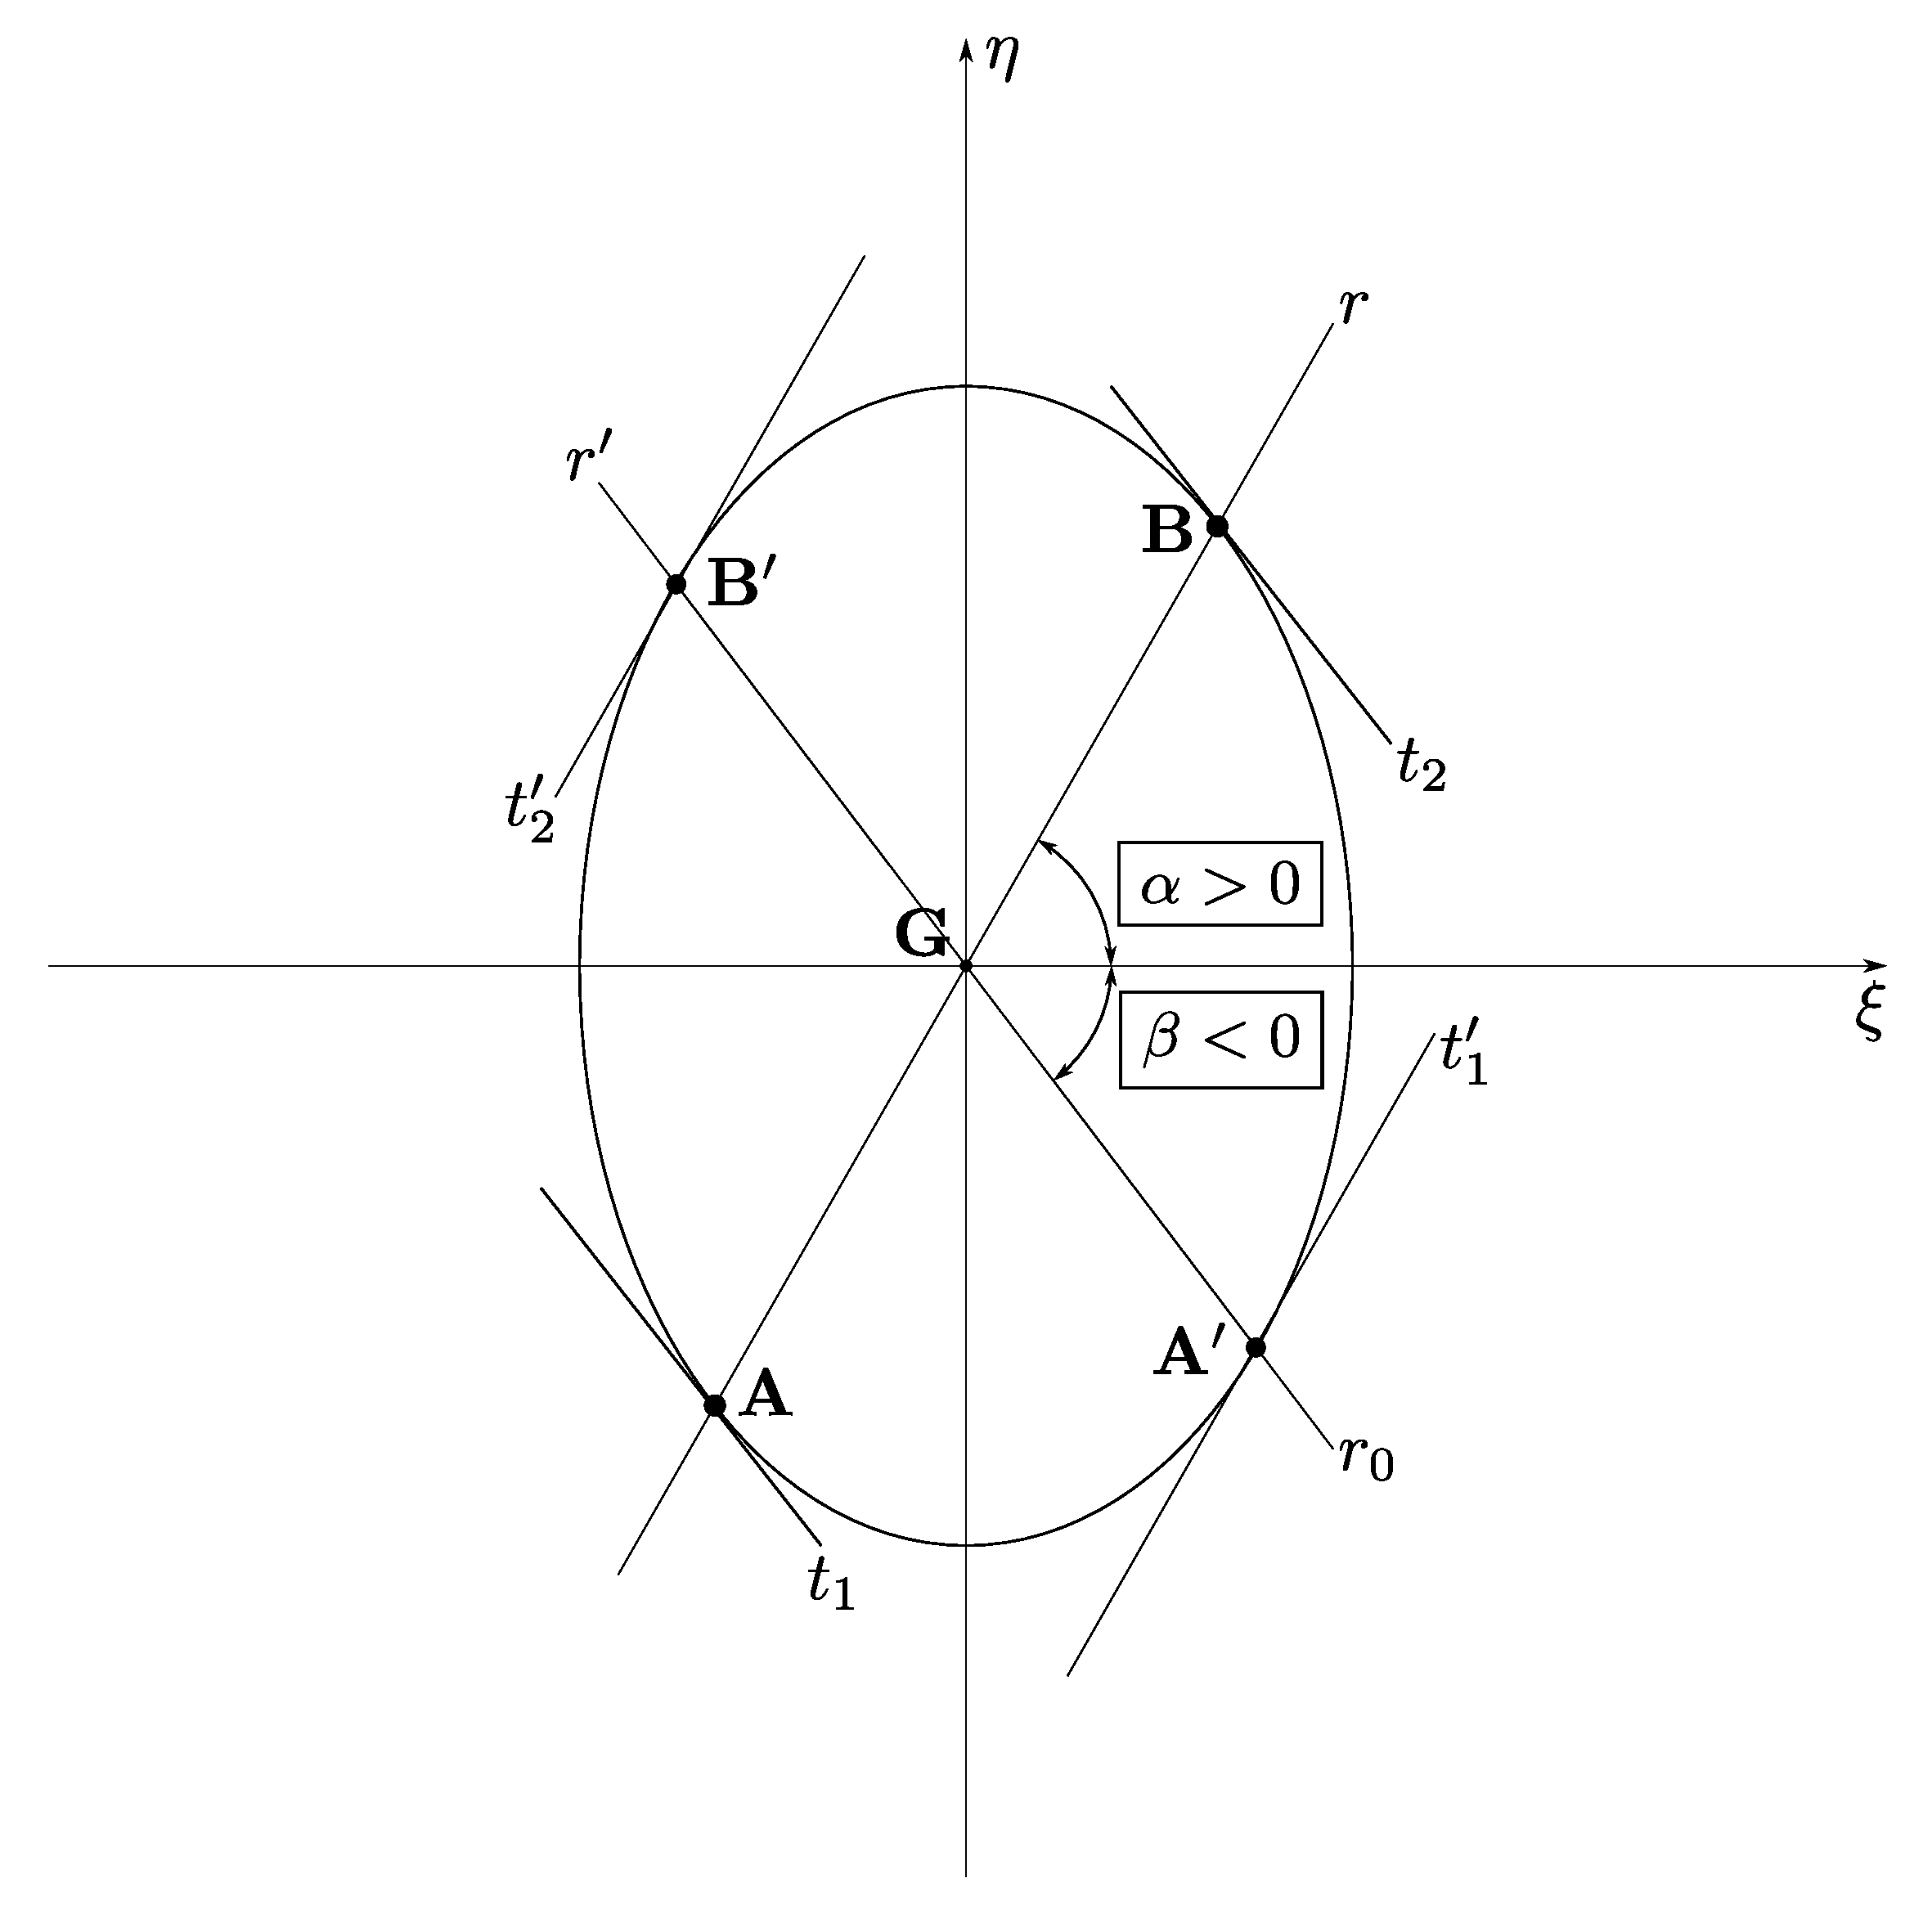
\includegraphics[width=0.75\textwidth]{Immagini/Parte_6/Figura6_2/Figura6_2.pdf}
\caption{}
\label{figura6-2}
\end{figure}
%--------------------------------------------------------------------------------------------------------------------------------------------------------------
Con riferimento alla figura~\ref{figura6-2}, $r$ è un qualunque diametro dell'ellisse ed $\mathbf{A}$ e $\mathbf{B}$ le sue intesezioni; osserviamo intanto che, per una nota proprietà dell'ellisse, le tangenti $t_1$ e $t_2$ sono parallele; $r'$ è il diametro parallelo a $t_1$ e $t_2$, $\mathbf{A}'$ e $\mathbf{B}'$ le sue intersezioni, $t_{1}'$ e $t_{2}'$ le rispettive tangenti. Ebbene, si può dimostrare analiticamente e constatare graficamente che  $t_{1}'$ e $t_{2}'$ sono parallele ad $r$. Ciò premesso, ogni coppia di diametri come $r$ ed $r'$, cioè tali che ognuno è parallelo alle tangenti agli estremi dell'altro, si dicono \textsc{diametri coniugati}. Si potrebbe dimostrare che, per ogni coppia di diametri coniugati, vale la seguente relazione 
%--------------------------------------------------------------------------------------------------------------------------------------------------------------
\begin{equation} \label{equazione6-3}
\boxed{\tan\alpha\cdot\tan\beta = -\frac{I_{\xi}}{I_{\eta}}}
\tag{6.3}
\end{equation}
%--------------------------------------------------------------------------------------------------------------------------------------------------------------
Il segno meno sta ad indicare che gli angoli $\alpha$ e $\beta$ hanno segno opposto, e cioè che i due diametri coniugati stanno sempre in quadranti diversi; in particolare, la figura~\ref{figura6-2}, $\alpha$ è positivo perché antiorario. 
%--------------------------------------------------------------------------------------------------------------------------------------------------------------

\noindent In ogni ellisse esistono chiaramente infinite coppie di diametri coniugati; gli assi principali di inerzia sono l'unica coppia di diametri coniugati \textsc{ortogonali}. Si potrebbe, infine, dimostrare che 
%--------------------------------------------------------------------------------------------------------------------------------------------------------------
\\

\fbox{\begin{minipage}{38em}
\centering
\textsc{Il momento centrifugo è nullo rispetto ad ogni coppia di diametri coniugati.}
\end{minipage}}
\\
\\

%--------------------------------------------------------------------------------------------------------------------------------------------------------------
\noindent In conseguenza di quest'ultima proposizione e in forza del teorema del trasporto del momento centrifugo, è immediato rendersi conto che, se $r_0$ ed $s_0$ sono una qualunque coppia di diametri coniugati, risulta
%--------------------------------------------------------------------------------------------------------------------------------------------------------------
\begin{equation*}
I_{rs_{0}} = I_{r_{0}s} = I_{r_{0}s_{0}} = 0, \qquad \forall r\,\parallelsum r_0 \quad e \quad \forall s\,\parallelsum s_0
\end{equation*}
%--------------------------------------------------------------------------------------------------------------------------------------------------------------
\section{Punti coniugati rispetto all'ellisse}
%----------------------------------------------------------------------------------------
\renewcommand{\thefigure}{6~-~3}
\begin{figure}[ht]
\centering
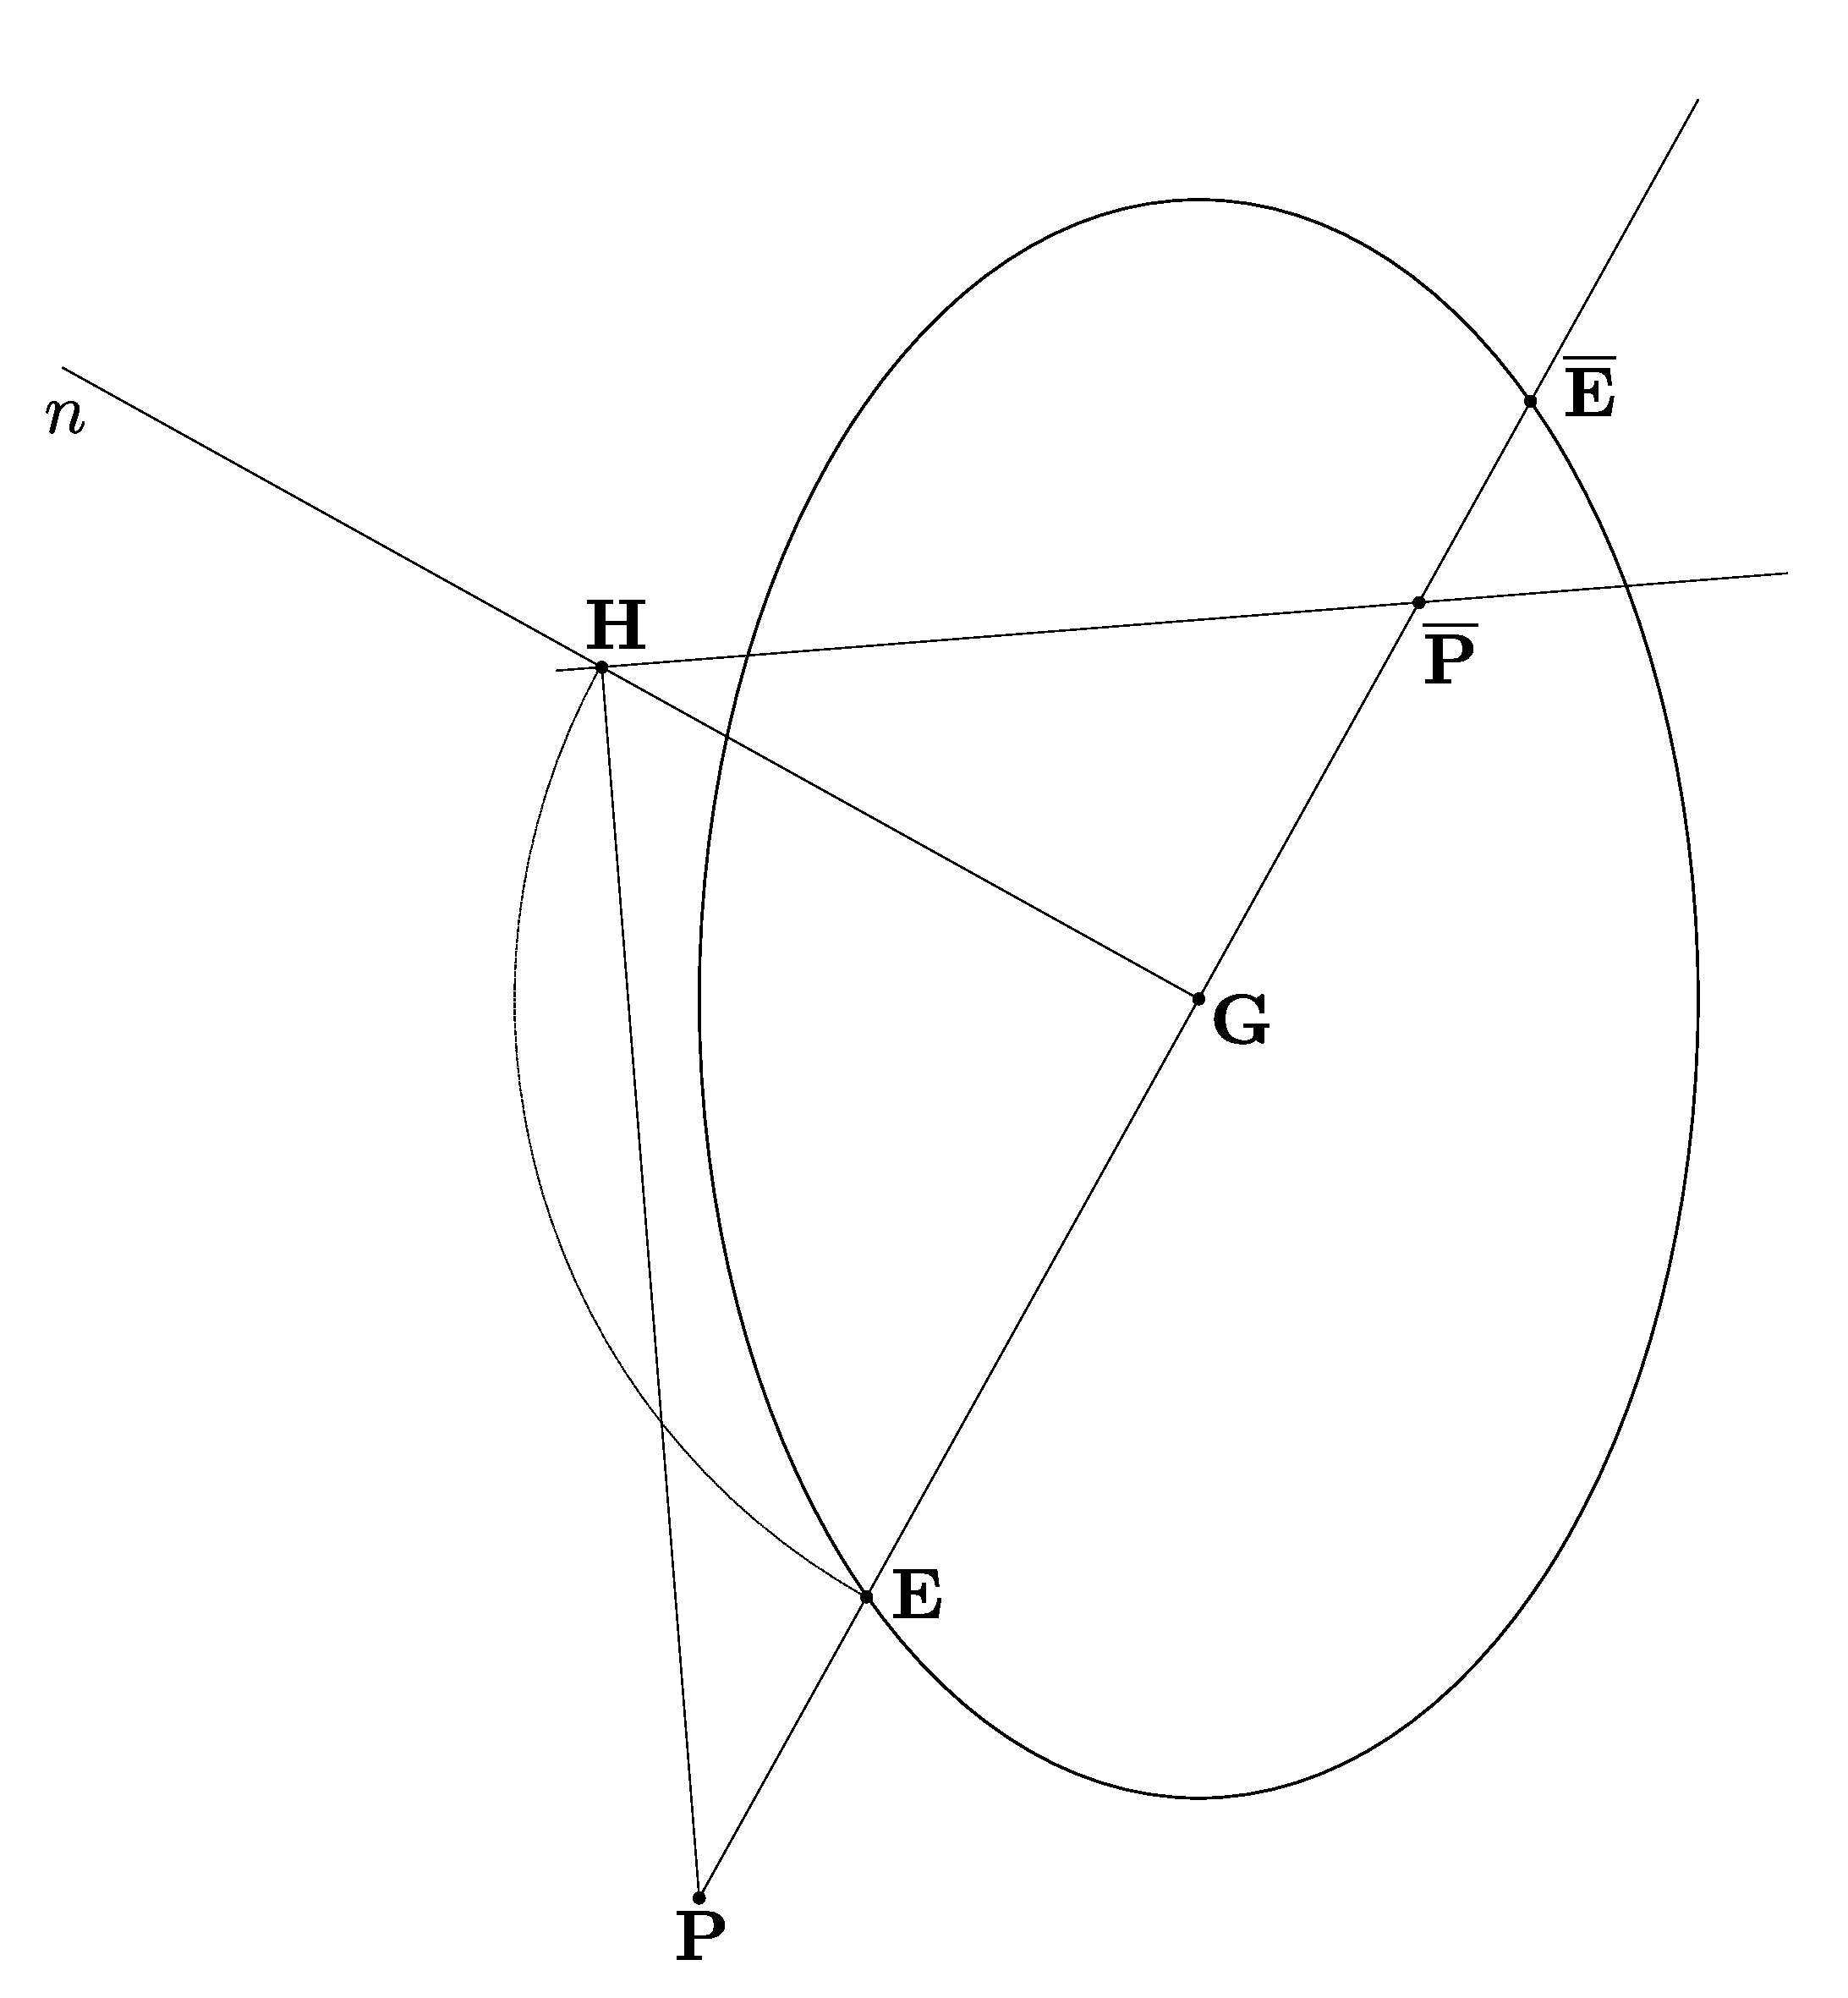
\includegraphics[width=0.75\textwidth]{Immagini/Parte_6/Figura6_3/Figura6_3.pdf}
\caption{}
\label{figura6-3}
\end{figure}
%--------------------------------------------------------------------------------------------------------------------------------------------------------------
Con riferimento alla figura~\ref{figura6-3}, sia $\mathbf{P}$ un punto qualunque del piano; si dice \textsc{coniugato di} $\mathbf{P}$, rispetto all'ellisse, il punto $\overline{\mathbf{P}}$ tale che 
%--------------------------------------------------------------------------------------------------------------------------------------------------------------
\begin{enumerate}
\item $\overline{\mathbf{P}}$ sta sul diametro $\mathbf{P}\mathbf{G}$;
\item $\overline{\mathbf{P}}$ sta dalla parte opposta di $\mathbf{P}$ rispetto a $\mathbf{G}$; 
\item vale la relazione 
%--------------------------------------------------------------------------------------------------------------------------------------------------------------
\begin{equation} \label{equazione6-4}
\lvert\,\mathbf{G}\mathbf{P}\,\lvert\,\lvert\,\mathbf{G}\overline{\mathbf{P}}\,\lvert = \lvert\,\mathbf{G}\mathbf{E}\,\lvert^2
\tag{6.4}
\end{equation}
%--------------------------------------------------------------------------------------------------------------------------------------------------------------
\end{enumerate}
%--------------------------------------------------------------------------------------------------------------------------------------------------------------
In figura~\ref{figura6-3} è illustrata la costruzione $\overline{\mathbf{P}}$
%--------------------------------------------------------------------------------------------------------------------------------------------------------------
\begin{enumerate}
\item si ribalta il raggio $\mathbf{G}\mathbf{E}$ sulla retta $n$ ad esso ortogonale; e dunque $\lvert\,\mathbf{G}\mathbf{H}\,\lvert = \lvert\,\mathbf{G}\mathbf{E}\,\lvert$;
\item si congiunge $\mathbf{P}$ con $\mathbf{H}$ e si traccia da $\mathbf{H}$ la perpendicolare $\mathbf{P}\mathbf{H}$; si interseca così in $\overline{\mathbf{P}}$ la retta $\mathbf{P}\mathbf{G}$.
\end{enumerate}
%--------------------------------------------------------------------------------------------------------------------------------------------------------------
Il secondo teorema di Euclide garantisce che il punto $\overline{\mathbf{P}}$ così determinato verifica la~\eqref{equazione6-4} ed è, pertanto, il coniugato di $\mathbf{P}$. 
%--------------------------------------------------------------------------------------------------------------------------------------------------------------

\noindent Alla luce della~\eqref{equazione6-4} appaiono, infine, ovvie, le seguenti proposizioni
%--------------------------------------------------------------------------------------------------------------------------------------------------------------
\\

\fbox{\begin{minipage}{38em}
\centering
\textsc{Il coniugato di un punto dell'ellisse, come $\mathbf{E}$, è il punto diametralmente opposto $\overline{\mathbf{E}}$.}
\end{minipage}}
\\
\\
%
%%--------------------------------------------------------------------------------------------------------------------------------------------------------------
%\\

\fbox{\begin{minipage}{38em}
\centering
\textsc{Più $\mathbf{P}$ si allontana da $\mathbf{G}$ e più il suo coniugato $\overline{\mathbf{P}}$ i avvicina a $\mathbf{G}$; se $\mathbf{P}$ è fuori dall'ellisse, $\overline{\mathbf{P}}$ si trova all'interno di quest'ultima.}
\end{minipage}}
\\
\\

%--------------------------------------------------------------------------------------------------------------------------------------------------------------
In particolare 
%--------------------------------------------------------------------------------------------------------------------------------------------------------------
\begin{align*}
\mathbf{P} &\rightarrow \infty \iff \overline{\mathbf{P}}\rightarrow \mathbf{G} \\
\mathbf{P} &\rightarrow \mathbf{G} \iff \overline{\mathbf{P}}\rightarrow \infty
\end{align*}
%--------------------------------------------------------------------------------------------------------------------------------------------------------------
\section{Antipolarità rispetto all'ellisse}
%----------------------------------------------------------------------------------------
\renewcommand{\thefigure}{6~-~4}
\begin{figure}[ht]
\centering
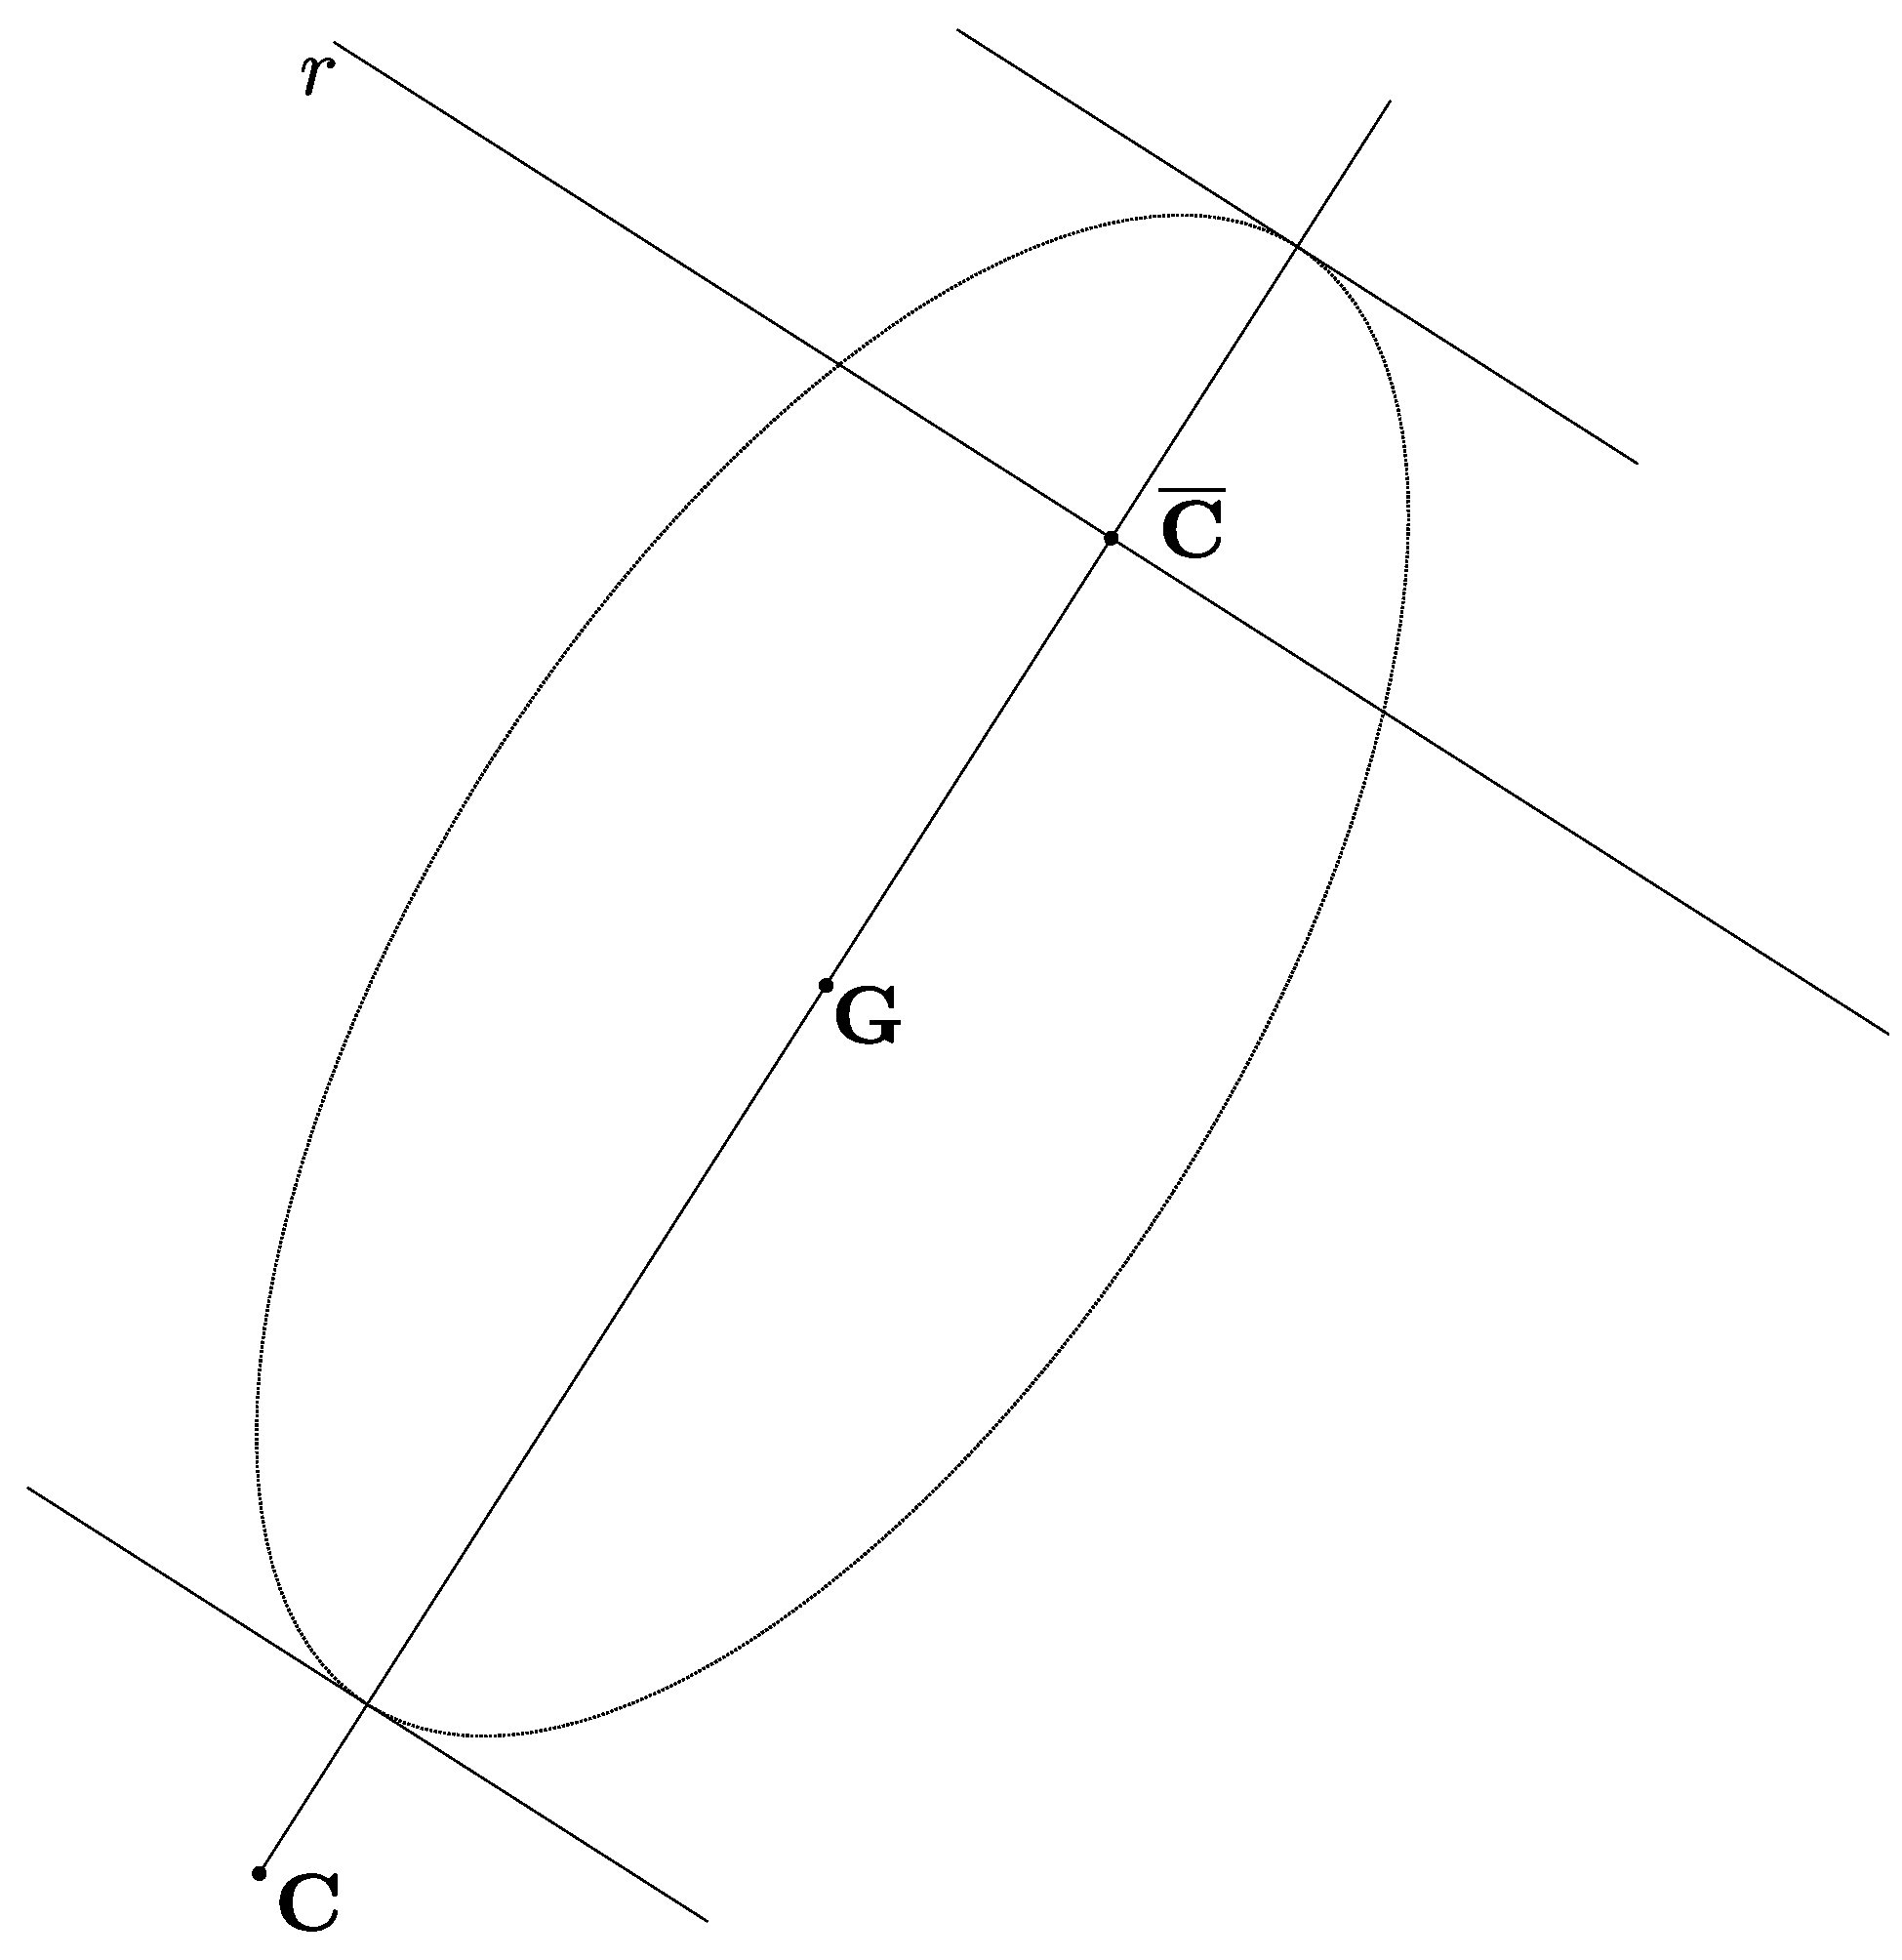
\includegraphics[width=0.75\textwidth]{Immagini/Parte_6/Figura6_4/Figura6_4.pdf}
\caption{}
\label{figura6-4}
\end{figure}
%--------------------------------------------------------------------------------------------------------------------------------------------------------------
Con riferimento alla~\ref{figura6-4}, sia $\mathbf{C}$ un punto e $\overline{\mathbf{C}}$ il suo coniugato; la retta $r$ passante per $\overline{\mathbf{C}}$ e avente direzione coniugata ala diametro $\mathbf{C}\mathbf{G}$ si dice \textsc{antipolare} del punto $\mathbf{C}$ rispetto all'ellisse. Sempre con riferimento alla~\ref{figura6-4}, sia $r$ una generica retta e $\overline{\mathbf{C}}$ l'intersezione di $r$ con il diametro ad essa coniugato; il punto $\mathbf{C}$, coniugato di $\overline{\mathbf{C}}$, si dice \textsc{antipolo} di $r$ rispetto all'ellisse. Resta così definita una corrispondenza fra l'insieme dei punti e l'insieme delle rette del piano
%--------------------------------------------------------------------------------------------------------------------------------------------------------------
\begin{equation*}
\boxed{\textup{\textsc{antipolo}}} \longleftrightarrow \boxed{\textup{\textsc{antipolare}}}
\end{equation*}
%--------------------------------------------------------------------------------------------------------------------------------------------------------------
e tale corrispondenza è chiaramente \textsc{invertibile} e prende il nome di \textsc{antipolarità}. 
%--------------------------------------------------------------------------------------------------------------------------------------------------------------
\noindent Dalla stessa definizione di antipolarità e per una ben nota proprietà dei punti coniugati, scaturisce la seguente proposizione 
%--------------------------------------------------------------------------------------------------------------------------------------------------------------
\\

\fbox{\begin{minipage}{38em}
\centering
\textsc{Più una retta si avvicina a $\mathbf{G}$, più il suo antipolo se ne allontana.}
\end{minipage}}
\\
\\

%--------------------------------------------------------------------------------------------------------------------------------------------------------------
\noindent In particolare: se $r$ passa per $\mathbf{G}$ il suo antipolo sarà il \textsc{punto improprio} in direzione del diametro coniugato ad $r$. 
%--------------------------------------------------------------------------------------------------------------------------------------------------------------

\noindent In geometria si studia che la \textsc{polare} del punto $\mathbf{C}(\xi_{C}, \eta_{C})$ rispetto all'ellisse di equazione~\eqref{equazione6-2} è la retta di equazione 
%--------------------------------------------------------------------------------------------------------------------------------------------------------------
\begin{equation*}
\boxed{\frac{\xi_C}{\rho_{\eta}^{2}}\xi+\frac{\eta_C}{\rho_{\xi}^{2}}\eta -1 = 0}
\end{equation*}
%--------------------------------------------------------------------------------------------------------------------------------------------------------------
In effetti, l'\textsc{antipolare} è la retta \textsc{simmetrica} della polare rispetto all'origine; la sua equazione è pertanto 
%--------------------------------------------------------------------------------------------------------------------------------------------------------------
\begin{equation} \label{equazione6-5}
\boxed{\textup{Equazione dell'antipolare del punto }\mathbf{C}(\xi_{C}, \eta_{C})} \rightarrow \boxed{\frac{\xi_C}{\rho_{\eta}^{2}}\xi+\frac{\eta_C}{\rho_{\xi}^{2}}\eta + 1 = 0}
\tag{6.5}
\end{equation}
%--------------------------------------------------------------------------------------------------------------------------------------------------------------
È dunque immediato, dato un punto, scrivere l'equazione della sua antipolare, e disegnarla rispetto agli assi principali. Ed è pure abbastanza agevole, data una retta $r$, trovare le coordinate del suo antipolo, sempre rispetto agli assi principali; ecco come si procede 
%--------------------------------------------------------------------------------------------------------------------------------------------------------------
\begin{enumerate}
\item si scrive l'equazione di $r$ nella forma 
%--------------------------------------------------------------------------------------------------------------------------------------------------------------
\begin{equation*}
a\xi+b\eta+1=0
\end{equation*}
%--------------------------------------------------------------------------------------------------------------------------------------------------------------
\item dal confronto con la~\eqref{equazione6-5} si ricava immediatamente che 
%--------------------------------------------------------------------------------------------------------------------------------------------------------------
\begin{equation} \label{equazione6-6}
\boxed{\eta_C = a\rho_{\eta}^{2} \quad ; \quad \eta_C = b\rho_{\xi}^{2}}
\tag{6.6}
\end{equation}
%--------------------------------------------------------------------------------------------------------------------------------------------------------------
\end{enumerate}
%--------------------------------------------------------------------------------------------------------------------------------------------------------------
\section{Il nocciolo centrale di inerzia}
%----------------------------------------------------------------------------------------
\renewcommand{\thefigure}{6~-~5}
\begin{figure}[ht]
\centering
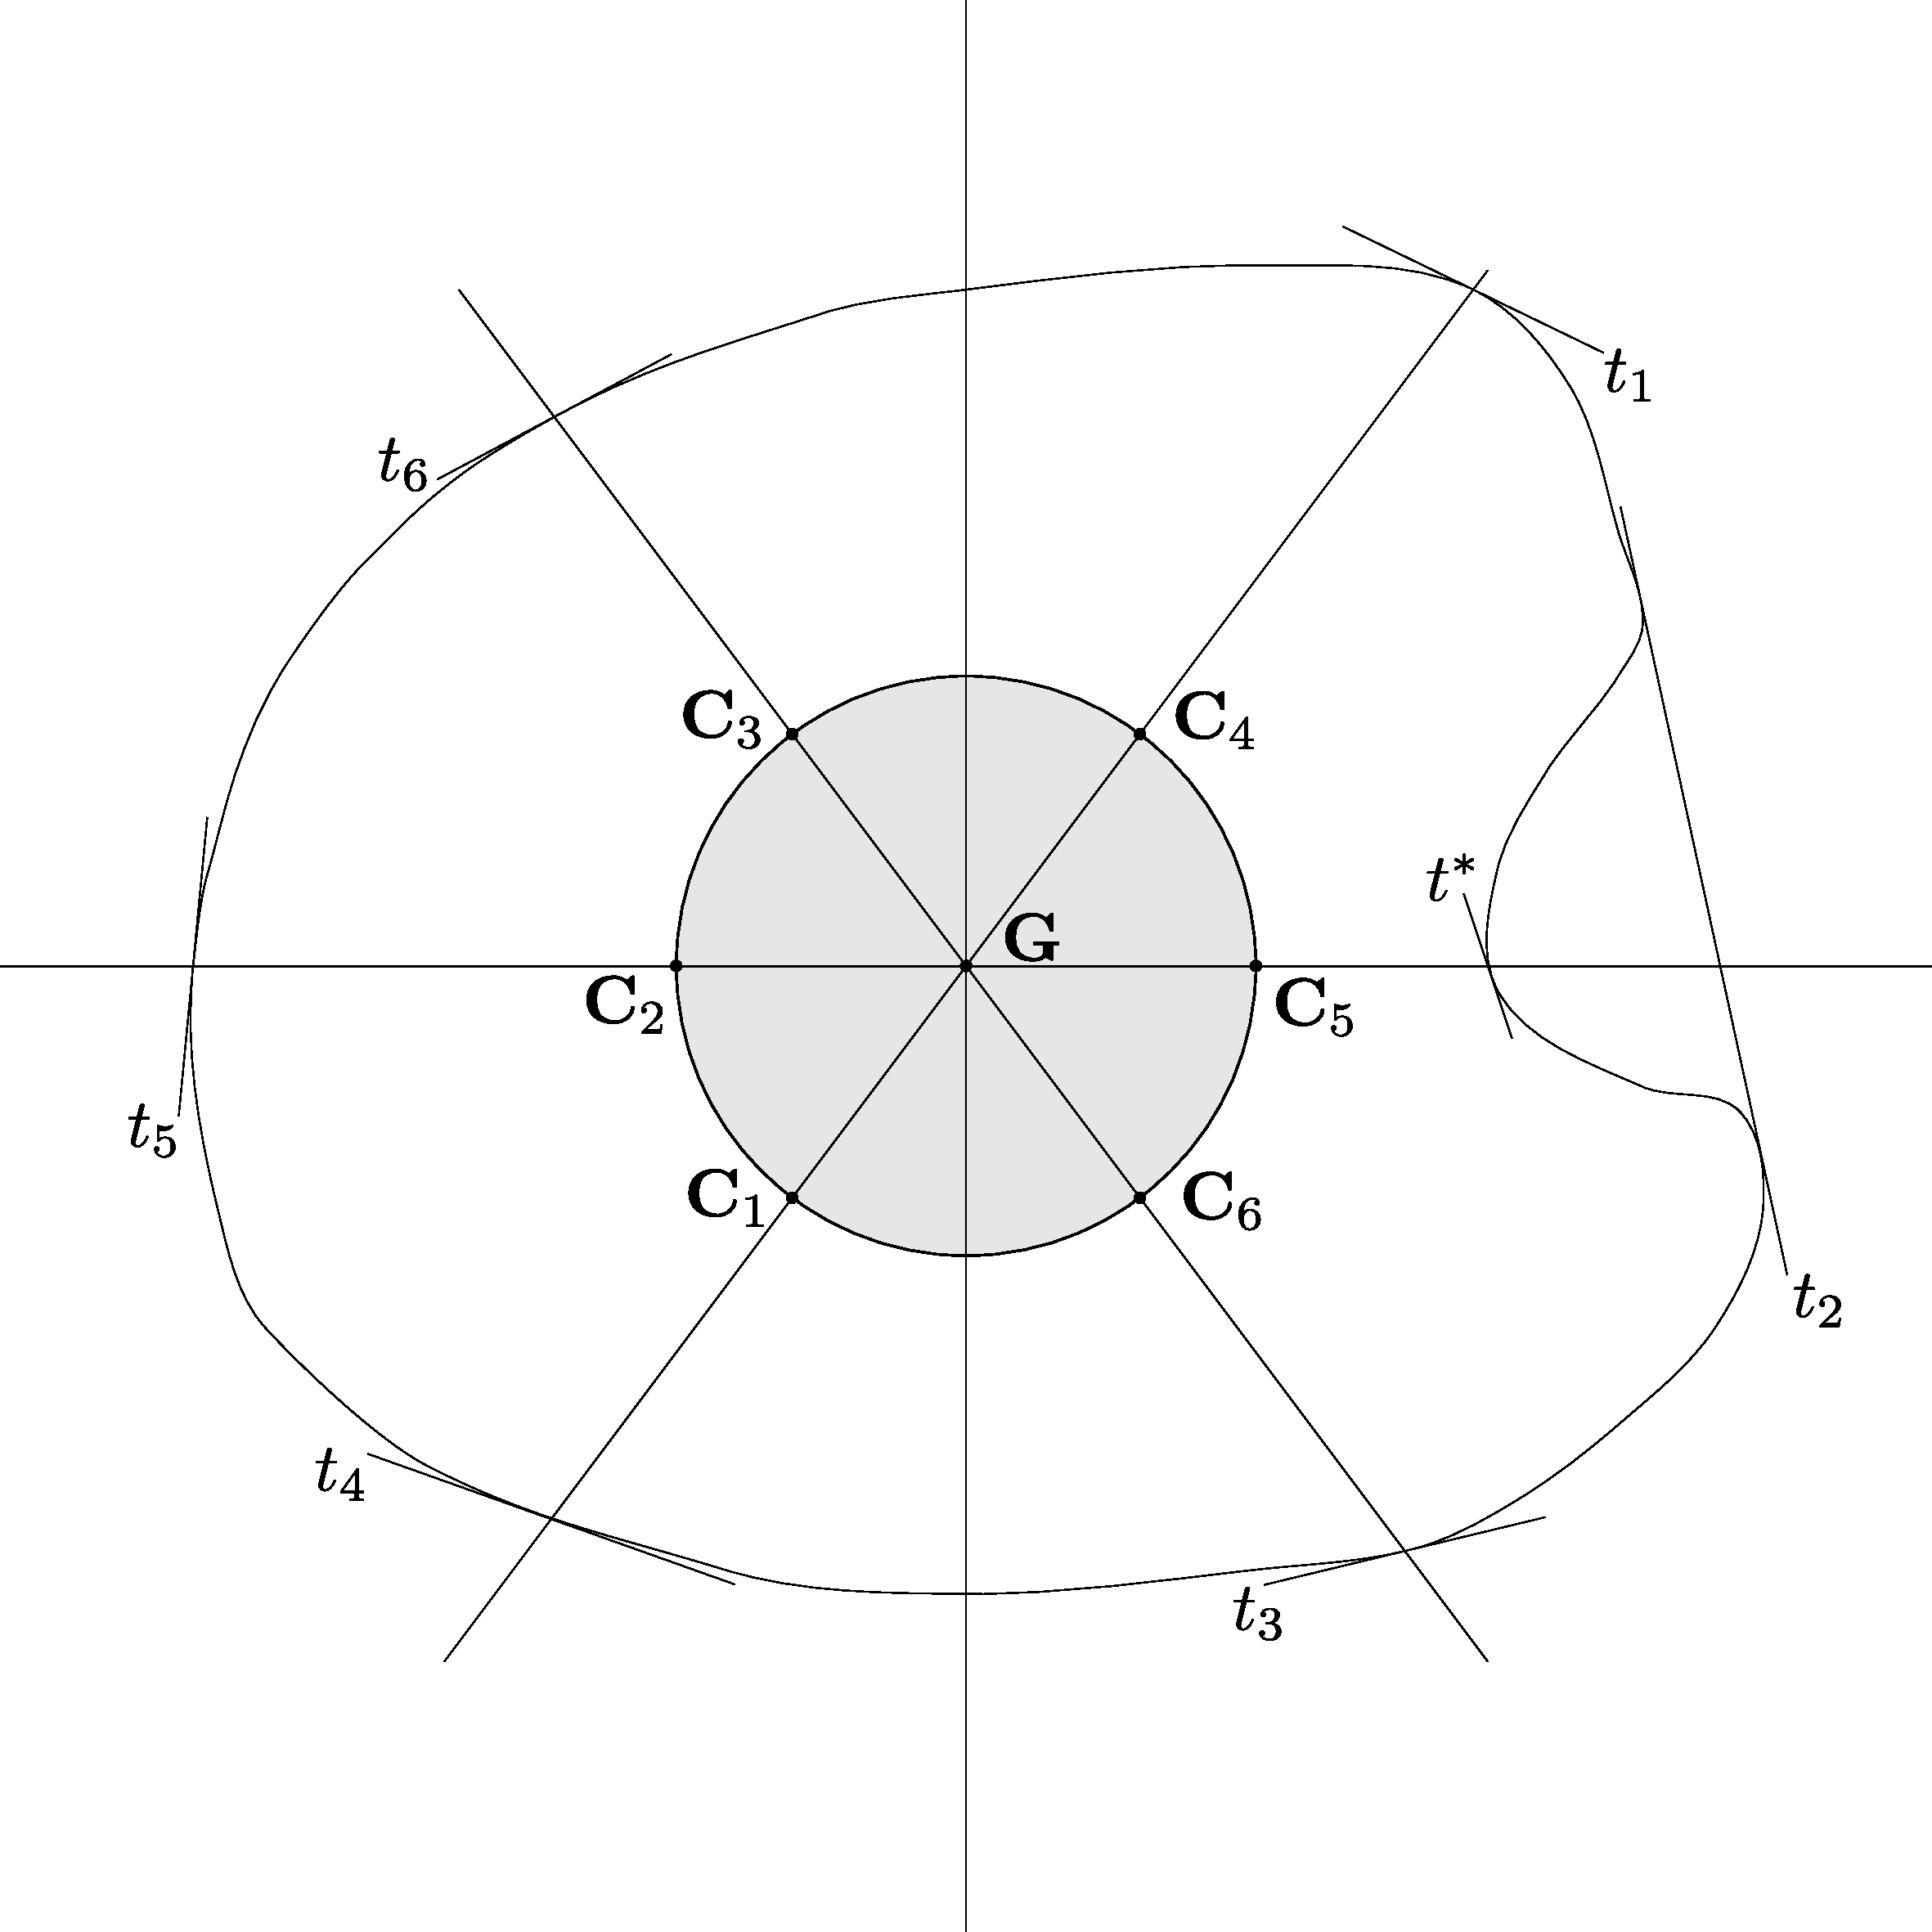
\includegraphics[width=0.75\textwidth]{Immagini/Parte_6/Figura6_5/Figura6_5.pdf}
\caption{}
\label{figura6-5}
\end{figure}
%--------------------------------------------------------------------------------------------------------------------------------------------------------------
\noindent In figura~\ref{figura6-5} è disegnata una generica figura piana; si ritengono noti, anche se non sono stati disegnati, gli assi principali di inerzia $\xi$ ed $\eta$ ed i relativi raggi di inerzia. 
%--------------------------------------------------------------------------------------------------------------------------------------------------------------

\noindent Si pensi alle infinite rette \textsc{tangenti al contorno} ma non secanti la figura: in figura~\ref{figura6-5} se ne sono disegnate soltanto sei; si osservi la retta $t^{*}$: essa, essendo secante la figura, non deve essere annoverata fra le tangenti al contorno.
%--------------------------------------------------------------------------------------------------------------------------------------------------------------

\noindent Di ogni retta tangente, ma non secante, si determini l'antipolo; in figura~\ref{figura6-5} si sono disegnati, solo qualitativamente, gli antipoli $\mathbf{C}_{1},\,\,\mathbf{C}_{2},\,\,\dots\,\,,\,\,\mathbf{C}_{6}$ rispettivamente delle rette $t_{1},\,\,t_{2},\,\,\dots\,\,,\,\,t_{6}$. Se si disegnassero tutti gli antipoli delle infinite rette tangenti, ma non secanti, si otterrebbe una curva, ovviamente chiusa, circondante il baricentro. La zona racchiusa dalla suddetta curva si dice \textsc{nocciolo centrale di inerzia} della figura piana. 
%--------------------------------------------------------------------------------------------------------------------------------------------------------------

\noindent Alla luce di quanto visto nel paragrafo precedente appare ovvia la seguente proposizione 
%--------------------------------------------------------------------------------------------------------------------------------------------------------------
\\

\fbox{\begin{minipage}{38em}
\centering
\textsc{Le rette esterne alla figura hanno antipolo interno al nocciolo e le rette secanti ce l'hanno esterno.}
\end{minipage}}
%--------------------------------------------------------------------------------------------------------------------------------------------------------------
\section{Nocciolo del cerchio}
%----------------------------------------------------------------------------------------
\renewcommand{\thefigure}{6~-~6}
\begin{figure}[ht]
\centering
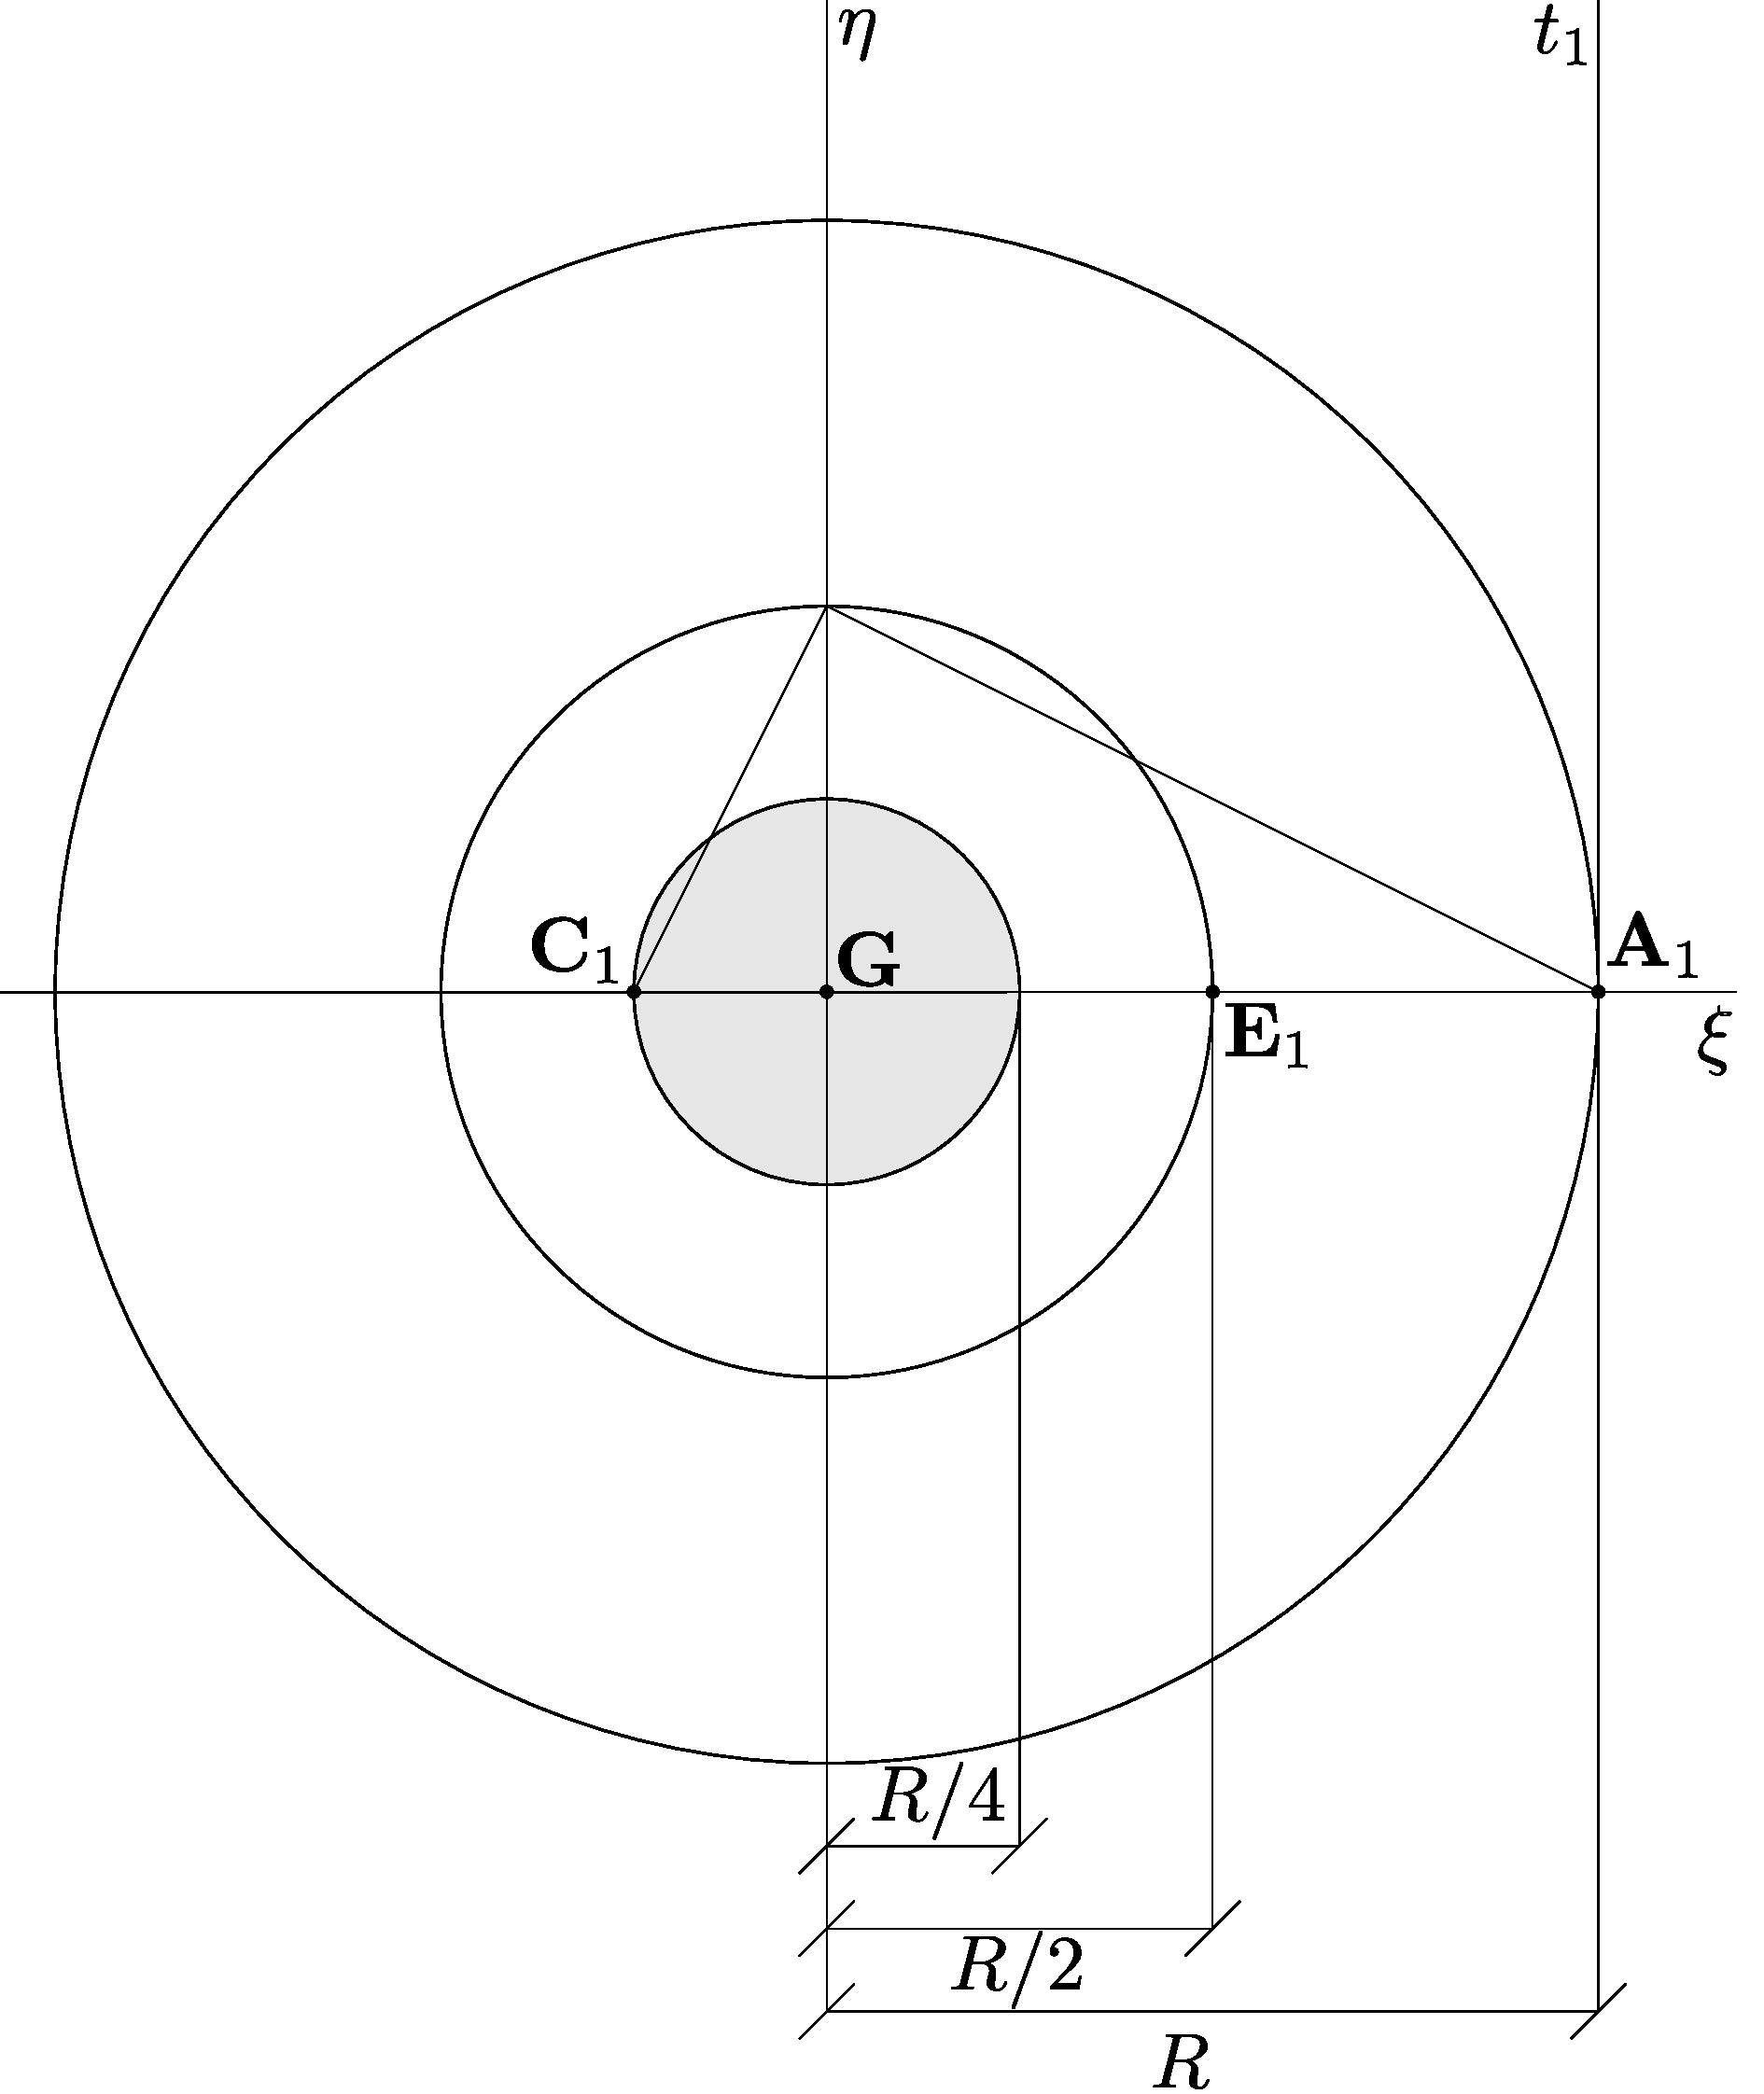
\includegraphics[width=0.51\textwidth]{Immagini/Parte_6/Figura6_6/Figura6_6.pdf}
\caption{}
\label{figura6-6}
\end{figure}
%--------------------------------------------------------------------------------------------------------------------------------------------------------------
\noindent In figura~\ref{figura6-6} è rappresentato un cerchio di raggio $R$. È noto che 
%--------------------------------------------------------------------------------------------------------------------------------------------------------------
\begin{align*}
A &= \pi R^2 \\ 
I_{\xi} &= I_{\eta} = \frac{\pi R^4}{4}
\end{align*}
%--------------------------------------------------------------------------------------------------------------------------------------------------------------
e quindi 
%--------------------------------------------------------------------------------------------------------------------------------------------------------------
\begin{equation*}
\rho_{\xi} = \rho_{\eta} = \frac{R}{2}
\end{equation*}
%--------------------------------------------------------------------------------------------------------------------------------------------------------------
L'ellisse centrale di inerzia del nostro cerchio è, pertanto, ancora un cerchio, ma di raggio $\frac{R}{2}$. 
%--------------------------------------------------------------------------------------------------------------------------------------------------------------

\noindent In figura~\ref{figura6-6} si è costruito l'antipolo $\mathbf{C}_1$ della retta $r_1$: $\mathbf{C}_1$ è ovviamente il coniugato di $\mathbf{A}_1$ e, per definizione di punti coniugati, si veda l'equazione~\eqref{equazione6-4}, risulta 
%--------------------------------------------------------------------------------------------------------------------------------------------------------------
\begin{equation*}
\lvert\,\mathbf{C}_{1}\mathbf{G}\,\lvert = \frac{\lvert\,\mathbf{G}\mathbf{E}_{1}\,\lvert^{2}}{\lvert\,\mathbf{G}\mathbf{A}_{1}\lvert} = \frac{\bigl(\frac{R}{2}\bigr)^2}{R} = \frac{R}{4}
\end{equation*}
%--------------------------------------------------------------------------------------------------------------------------------------------------------------
È immediato convincersi che, per evidenti ragioni di simmetria, tutte le tangenti del cerchio hanno l'antipolo equidistante da $\mathbf{G}$; il nocciolo centrale di inerzia è pertanto un cerchio di raggio $\frac{R}{4}$.
%--------------------------------------------------------------------------------------------------------------------------------------------------------------
\section{Il nocciolo del rettangolo}
%----------------------------------------------------------------------------------------
\renewcommand{\thefigure}{6~-~7}
\begin{figure}[ht]
\centering
\includegraphics[width=0.51\textwidth]{Immagini/Parte_6/Figura6_7/Figura6_7.pdf}
\caption{}
\label{figura6-7}
\end{figure}
%--------------------------------------------------------------------------------------------------------------------------------------------------------------
\noindent È noto che 
%--------------------------------------------------------------------------------------------------------------------------------------------------------------
\begin{align*}
A &= bh \\ 
I_{\xi} &= \frac{bh^{3}}{12} \\
I_{\eta} &= \frac{b^{3}h}{12}
\end{align*}
%--------------------------------------------------------------------------------------------------------------------------------------------------------------
e dunque 
%--------------------------------------------------------------------------------------------------------------------------------------------------------------
\begin{align*}
\rho_{\xi} &= \frac{h}{\sqrt{12}} \\
\rho_{\eta} &= \frac{b}{\sqrt{12}}
\end{align*}
%--------------------------------------------------------------------------------------------------------------------------------------------------------------
\noindent Abbiamo potuto, così, disegnare i due diametri principali dell'ellisse centrale di inerzia. 
%--------------------------------------------------------------------------------------------------------------------------------------------------------------

\noindent Il contorno del nocciolo è, ovviamente, costituito dagli antipoli delle quattro rette $t_{1}$, $t_{2}$, $t_{3}$ e $t_{4}$, coincidenti con i lati, nonché delle infinite rette come $r$ passanti per i vertici e non secanti. 
%--------------------------------------------------------------------------------------------------------------------------------------------------------------

\noindent L'antipolo $\mathbf{C}_{1}$ di $t_1$ è, ovviamente, il coniugato di $\mathbf{A}_{1}$ e perciò
%--------------------------------------------------------------------------------------------------------------------------------------------------------------
\begin{equation*}
\lvert\,\mathbf{G}\mathbf{C}_{1}\,\lvert = \frac{\rho_{\xi}^{2}}{\lvert\,\mathbf{G}\mathbf{A}_{1}\,\lvert} = \frac{h}{6}
\end{equation*}
%--------------------------------------------------------------------------------------------------------------------------------------------------------------
\noindent L'antipolo $\mathbf{C}_{2}$ di $t_2$ è il coniugato di $\mathbf{A}_{2}$ 
%--------------------------------------------------------------------------------------------------------------------------------------------------------------
\begin{equation*}
\lvert\,\mathbf{G}\mathbf{C}_{2}\,\lvert = \frac{\rho_{\eta}^{2}}{\lvert\,\mathbf{G}\mathbf{A}_{2}\,\lvert} = \frac{b}{6}
\end{equation*}
%--------------------------------------------------------------------------------------------------------------------------------------------------------------
\noindent Gli antipoli $\mathbf{C}_{3}$ e $\mathbf{C}_{4}$ delle rette $t_3$ e $t_4$ sono, ovviamente, i simmetrici di $\mathbf{C}_{1}$ e di $\mathbf{C}_{2}$.
%----------------------------------------------------------------------------------------
\renewcommand{\thefigure}{6~-~8}
\begin{figure}[ht]
\centering
\includegraphics[width=0.51\textwidth]{Immagini/Parte_6/Figura6_8/Figura6_8.pdf}
\caption{}
\label{figura6-8}
\end{figure}
%--------------------------------------------------------------------------------------------------------------------------------------------------------------
Per quanto riguarda gli antipoli delle rette passanti per $\mathbf{V}$, si può dimostrare che essi si trovano sul segmento $\mathbf{C}_{1}\mathbf{C}_{2}$; analogamente, può dirsi per le rette passanti per gli altri vertici. Il nocciolo del rettangolo è, dunque, il \textsc{rombo} le cui diagonali sono lunghe $\frac{1}{3}$ dei lati paralleli, come mostrato in figura~\ref{figura6-8}.
%--------------------------------------------------------------------------------------------------------------------------------------------------------------
\section{Il nocciolo di un profilato}
%--------------------------------------------------------------------------------------------------------------------------------------------------------------
\renewcommand{\thefigure}{6~-~9}
\begin{figure}[ht]
\centering
\subfloat[][]
{\includegraphics[width=.35\textwidth]{Immagini/Parte_6/Figura6_9/Figura6_9a.pdf}} \quad
\subfloat[][]
{\includegraphics[width=.35\textwidth]{Immagini/Parte_6/Figura6_9/Figura6_9b.pdf}} \\
\subfloat[][]
{\includegraphics[width=.35\textwidth]{Immagini/Parte_6/Figura6_9/Figura6_9c.pdf}} \quad
\subfloat[][]
{\includegraphics[width=.35\textwidth]{Immagini/Parte_6/Figura6_9/Figura6_9d.pdf}}
\caption{}
\label{figura6-9}
\end{figure}
%--------------------------------------------------------------------------------------------------------------------------------------------------------------
Per disegnare il nocciolo di un profilato occorre e basta determinare gli antipoli di un numero finito di rette, quelle che lambiscono senza intersecare, giacché nei vertici resta valido quanto detto per il rettangolo.
%--------------------------------------------------------------------------------------------------------------------------------------------------------------

\noindent Il nocciolo di un profilato è pertanto un poligono a quattro o più vertici. Nella figura~\ref{figura6-9} sono mostrati, qualitativamente, i noccioli di alcuni fra i tipi più comuni di profilati.
%--------------------------------------------------------------------------------------------------------------------------------------------------------------
\clearpage
\section{Esercizi}
\paragraph{Esercizio 6.1}
Determinare il nocciolo del profilato riportato in figura, dove è disegnata solo la linea media.
%--------------------------------------------------------------------------------------------------------------------------------------------------------------
\renewcommand{\thefigure}{6.1~-~1}
\begin{figure}[ht]
\centering
\includegraphics[width=0.75\textwidth]{Immagini/Parte_6/Esercizio6_1/Esercizio6_1_1.pdf}
\caption{}
\label{Esercizio6-1-1}
\end{figure}
%--------------------------------------------------------------------------------------------------------------------------------------------------------------

\noindent Dalla figura si evince che $\tan\alpha=\frac{1}{2}$ e dunque 
%--------------------------------------------------------------------------------------------------------------------------------------------------------------
\begin{align*}
\sin\alpha &= \frac{1}{\sqrt{5}} \\
\cos\alpha &= \frac{2}{\sqrt{5}} \\
\lvert\, DE\,\lvert &= 8\sqrt{5} \approx 17.89\,\textup{cm} \\ 
\alpha &= 25.565^{\circ}
\end{align*}
%--------------------------------------------------------------------------------------------------------------------------------------------------------------
Scelto il riferimento iniziale con assi $x$ ed $y$, calcoliamo le coordinate del baricentro cone note formule
%--------------------------------------------------------------------------------------------------------------------------------------------------------------
%----------------------------------------------------------------------------------------
\begin{equation*}
\begin{aligned}
A_1 &=28\times2 = 56\,\textup{cm}^2 \\
A_2 &=24\times1.6 = 38.400\,\textup{cm}^2 \\
A_3 &=16\sqrt{5} = 35.777\,\textup{cm}^2
\end{aligned}
\,\,\Biggr\}\,\, A = 130.177\,\textup{cm}^2
\end{equation*}
%----------------------------------------------------------------------------------------
\begin{equation*}
\begin{aligned}
S_{1x} &= 0\,\textup{cm}^3 \\
S_{2x} &= 38.4\times12 = 460.800\,\textup{cm}^3 \\
S_{3x} &= 16\sqrt{5}\times 28  = 1001.758\,\textup{cm}^3
\end{aligned}
\,\,\Biggr\}\,\, S_x = 1462.558\,\textup{cm}^3
\end{equation*}
%----------------------------------------------------------------------------------------
\begin{equation*}
\begin{aligned}
S_{1y} &= 56\times(-2) = -112\,\textup{cm}^3 \\
S_{2y} &= 0\,\textup{cm}^3 \\
S_{3y} &= 16\sqrt{5}\times 8  = 286.217\,\textup{cm}^3
\end{aligned}
\,\,\Biggr\}\,\, S_y = 174.217\,\textup{cm}^3
\end{equation*}
%----------------------------------------------------------------------------------------
%--------------------------------------------------------------------------------------------------------------------------------------------------------------
e quindi si ottiene
%--------------------------------------------------------------------------------------------------------------------------------------------------------------
%----------------------------------------------------------------------------------------
\begin{equation*}
\boxed{
x_G = \frac{S_y}{A} = \frac{174.217}{130.177} = 1.338\,\textup{cm}
}
\end{equation*}
%----------------------------------------------------------------------------------------
\begin{equation*}
\boxed{
y_G = \frac{S_x}{A} = \frac{1462.558}{130.177} = 11.235\,\textup{cm}
}
\end{equation*}
%----------------------------------------------------------------------------------------
%--------------------------------------------------------------------------------------------------------------------------------------------------------------
Ora calcoleremo prima $I_x$, $I_y$ e $I_{xy}$ e poi, mediante i teoremi del trasporto, risaliremo ad $I_{x_0}$, $I_{y_0}$ ed $I_{x_{0}y_{0}}$, avendo indicato con $x_0$ ed $y_0$ le rette passanti per $\mathbf{G}$ parallele ad $x$ ed $y$. Conviene, però, fare alcune considerzioni preliminari sul rettangolo $\lvert\,DE\,\lvert$.
%--------------------------------------------------------------------------------------------------------------------------------------------------------------
\renewcommand{\thefigure}{6.1~-~2}
\begin{figure}[ht]
\centering
\includegraphics[width=0.53\textwidth]{Immagini/Parte_6/Esercizio6_1/Esercizio6_1_2.pdf}
\caption{}
\label{Esercizio6-1-2}
\end{figure}
%--------------------------------------------------------------------------------------------------------------------------------------------------------------
\begin{align*}
I_a &= \frac{8\sqrt{5}\times2^{3}}{12} = 12\,\textup{cm}^4 \\
I_b &= \frac{2\times(8\sqrt{5})^{3}}{12} = 954\,\textup{cm}^4
\end{align*}
%--------------------------------------------------------------------------------------------------------------------------------------------------------------
Ora valuteremo $I_c$, $I_d$ e $I_{cd}$ applicando le formule di trasformazione~\eqref{equazione4-1} ponendo in esse $\varphi=-\alpha$ ed identificando $I_x$ con $I_a$, $I_y$ con $I_b$ ed $I_{xy}$ con $I_{ab}=0$. Abbiamo dunque 
%--------------------------------------------------------------------------------------------------------------------------------------------------------------
\begin{align*}
\sin^{2}\varphi &= \sin^{2}\alpha = \frac{1}{5} \\
\cos^{2}\varphi &= \cos^{2}\alpha = \frac{4}{5} \\ 
\sin2\varphi &= -\sin2\alpha = -2\sin\alpha\cos\alpha = -2\frac{1}{\sqrt{5}}\frac{2}{\sqrt{5}} = -\frac{4}{5}
\end{align*}
%--------------------------------------------------------------------------------------------------------------------------------------------------------------
\begin{align*}
I_c &= I_{a}\cos^{2}\varphi+I_{b}\sin^{2}\varphi = 12\frac{4}{5}+954\frac{1}{5} = 200\,\textup{cm}^4 \\
I_d &= I_{a}\sin^{2}\varphi+I_{b}\cos^{2}\varphi = 12\frac{1}{5}+954\frac{4}{5} = 766\,\textup{cm}^4 \\
I_{cd} &= \frac{I_{a}-I_{b}}{2}\sin2\varphi = \frac{12-954}{2}\biggl(-\frac{4}{5}\biggr) = 377\,\textup{cm}^4
\end{align*}
%--------------------------------------------------------------------------------------------------------------------------------------------------------------
Ed ora passiamo al calcolo di $I_x$, $I_y$ e $I_{xy}$:
%--------------------------------------------------------------------------------------------------------------------------------------------------------------
%----------------------------------------------------------------------------------------
\begin{equation*}
\begin{aligned}
I_{1x} &= \frac{28\times2^{3}}{12} = 19\,\textup{cm}^4 \\
I_{2x} &= \frac{1.6\times24^{3}}{3} = 7373\,\textup{cm}^4 \\
I_{3x} &= I_c+A_{3}y_{G_3}^{2} = 200+16\sqrt{5}\times28^2 = 28249\,\textup{cm}^4 
\end{aligned}
\,\,\Biggr\}\,\, I_x = 35641\,\textup{cm}^4
\end{equation*}
%----------------------------------------------------------------------------------------
\begin{equation*}
\begin{aligned}
I_{1y} &= \frac{2\times28^{3}}{12} + 56\times2^2= 3883\,\textup{cm}^4 \\
I_{2y} &= \frac{24\times1.6^{3}}{12} = 8\,\textup{cm}^4 \\
I_{3y} &= I_d+A_{3}x_{G_3}^{2} = 766+16\sqrt{5}\times8^2 = 3056\,\textup{cm}^4 
\end{aligned}
\,\,\Biggr\}\,\, I_y = 6947\,\textup{cm}^4
\end{equation*}
%----------------------------------------------------------------------------------------
\begin{equation*}
\begin{aligned}
I_{1xy} &= 0 \\
I_{2xy} &= 0 \\
I_{3xy} &= I_{cd}+A_{3}x_{G_3}y_{G_3} = 377 + 16\sqrt{5}\times8\times28 = 8391\,\textup{cm}^4 
\end{aligned}
\,\,\Biggr\}\,\, I_y = 8391\,\textup{cm}^4
\end{equation*}
%----------------------------------------------------------------------------------------
%--------------------------------------------------------------------------------------------------------------------------------------------------------------
E finalmente calcoliamo  $I_{x_{0}}$, $I_{y_{0}}$ e $I_{x_{0}y_{0}}$
%--------------------------------------------------------------------------------------------------------------------------------------------------------------
\begin{align*}
I_{x_{0}} &= I_x - Ay_{G}^{2} = 35641-130.177\times11.235^{2} = 19209\,\textup{cm}^4 \\
I_{y_{0}} &= I_y - Ax_{G}^{2} = 6947-130.177\times1.338^{2} = 6714\,\textup{cm}^4 \\
I_{x_{0}y_{0}} &= I_{xy}-Ax_{G}y_{G} = 8391-130.177\times1.338\times11.235 = 6434\,\textup{cm}^4
\end{align*}
%--------------------------------------------------------------------------------------------------------------------------------------------------------------
Ora calcoliamo l'angolo $\varphi^{*}=\widehat{\xi x_{0}}$ 
%--------------------------------------------------------------------------------------------------------------------------------------------------------------
\begin{equation*}
\tan2\varphi^{*}=\frac{2I_{x_{0}y_{0}}}{I_{y_{0}}-I_{x_{0}}} = \frac{2\times6434}{6714-19209} \longrightarrow \tan2\varphi^{*}=-1.02985
\end{equation*}
%--------------------------------------------------------------------------------------------------------------------------------------------------------------
e dunque 
%--------------------------------------------------------------------------------------------------------------------------------------------------------------
\begin{equation*}
2\varphi^{*} = -45.84^{\circ} \longrightarrow \boxed{\varphi^{*}=-22.92^{\circ}}
\end{equation*}
%--------------------------------------------------------------------------------------------------------------------------------------------------------------
I valori di $I_{\xi}$ ed $I_{\eta}$ si possono ottenere utilizzando la~\eqref{equazione5-2a} come segue
%--------------------------------------------------------------------------------------------------------------------------------------------------------------
\begin{equation*}
\begin{aligned}
I_{\xi} & \\
I_{\eta} &
\end{aligned}
\,\,\Biggr\}\,\, \frac{I_{x}+I_{y}}{2} \pm \sqrt{\biggl(\frac{I_{x}-I_{y}}{2}\biggr)^{2}+I_{xy}^{2}}=12961\pm8968
\end{equation*}
%--------------------------------------------------------------------------------------------------------------------------------------------------------------
e quindi
%--------------------------------------------------------------------------------------------------------------------------------------------------------------
\begin{align*}
I_{\xi} &= 21929\,\textup{cm}^{4} \\
I_{\eta} &= 3993\,\textup{cm}^{4}
\end{align*}
%--------------------------------------------------------------------------------------------------------------------------------------------------------------
I raggi principali di inerzia valgono, dunque
%--------------------------------------------------------------------------------------------------------------------------------------------------------------
\begin{align*}
\rho_{\xi}^{2} &= \frac{I_{\xi}}{A} = \frac{21929}{130.177} = 168.455\,\textup{cm}^{2} \\
\rho_{\eta}^{2} &= \frac{I_{\eta}}{A} = \frac{3993}{130.177} = 30.674\,\textup{cm}^{2}
\end{align*}
%--------------------------------------------------------------------------------------------------------------------------------------------------------------
Il nocciolo del nostro profilato avrà per vertici gli antipoli delle rette $\mathbf{A}\mathbf{C}$, $\mathbf{A}\mathbf{D}$, $\mathbf{C}\mathbf{E}$, $\mathbf{D}\mathbf{E}$ e sarà, pertanto, un quadrilatero.
%--------------------------------------------------------------------------------------------------------------------------------------------------------------
Ricaveremo le coordinate degli antipoli delle quattro rette suddette utilizzando le~\eqref{equazione6-5}. Naturalmente dobbiamo scrivere le equazioni delle quattro rette suddette nel riferimento $\mathbf{G}\xi\eta$; e, a tale scopo, abbiamo bisogno delle coordinate dei punti $\mathbf{A}$, $\mathbf{C}$, $\mathbf{D}$, $\mathbf{E}$ nello stesso riferimento. Intanto, nel riferimento $\mathbf{G}x_{0}y_{0}$ i punti in questione hanno coordinate
%--------------------------------------------------------------------------------------------------------------------------------------------------------------
\begin{align*}
x_{0A} &= -17.338\,\textup{cm} \\ 
y_{0A} &= -11.235\,\textup{cm} 
\end{align*}
%--------------------------------------------------------------------------------------------------------------------------------------------------------------
\begin{align*}
x_{0D} &= -1.338\,\textup{cm} \\ 
y_{0D} &= 12.765\,\textup{cm} 
\end{align*}
%--------------------------------------------------------------------------------------------------------------------------------------------------------------
\begin{align*}
x_{0C} &= 10.662\,\textup{cm} \\ 
y_{0C} &= -11.235\,\textup{cm} 
\end{align*}
%--------------------------------------------------------------------------------------------------------------------------------------------------------------
\begin{align*}
x_{0E} &= 14.662\,\textup{cm} \\ 
y_{0E} &= 20.765\,\textup{cm} 
\end{align*}
%--------------------------------------------------------------------------------------------------------------------------------------------------------------
Nel riferimento $\mathbf{G}\xi\eta$, le coordinate dei quattro punti in questione si possono ricavare mediante le formule di trasformazione delle coordinate
%--------------------------------------------------------------------------------------------------------------------------------------------------------------
\begin{align*}
\xi &= x_{0}\cos\varphi^{*}+y_{0}\sin\varphi^{*} \\ 
\eta &= -x_{0}\sin\varphi^{*}+y_{0}\cos\varphi^{*}
\end{align*}
%--------------------------------------------------------------------------------------------------------------------------------------------------------------
Nella fattispecie, daremo le coordinate dei punti $\mathbf{C}_2$ e $\mathbf{C}_3$. Si ha
%--------------------------------------------------------------------------------------------------------------------------------------------------------------
\begin{equation*}
r_2 \longrightarrow \frac{28.336}{236.358}\xi - \frac{5.390}{236.358}\eta + 1 = 0
\end{equation*}
%--------------------------------------------------------------------------------------------------------------------------------------------------------------
e dunque le coordinate di $\mathbf{C}_2$ sono 
%--------------------------------------------------------------------------------------------------------------------------------------------------------------
\begin{align*}
\xi_{C_{2}} &= \frac{28.336}{236.358}30.674 = 3.617\,\textup{cm} \\ 
\eta_{C_{2}} &= -\frac{5.390}{236.358}168.455 = -3.841\,\textup{cm}
\end{align*}
%--------------------------------------------------------------------------------------------------------------------------------------------------------------
Passiamo alla retta $CE = r_3$ 
%--------------------------------------------------------------------------------------------------------------------------------------------------------------
\begin{equation*}
r_3 \longrightarrow (\xi - 14.196)31.032 = (\eta+6.196)(-8.779)
\end{equation*}
%--------------------------------------------------------------------------------------------------------------------------------------------------------------
E dunque 
%--------------------------------------------------------------------------------------------------------------------------------------------------------------
\begin{equation*}
r_3 \longrightarrow -\frac{31.032}{386.135}\xi - \frac{8.779}{386.135}\eta + 1 = 0
\end{equation*}
%--------------------------------------------------------------------------------------------------------------------------------------------------------------
e dunque le coordinate di $\mathbf{C}_3$ sono 
%--------------------------------------------------------------------------------------------------------------------------------------------------------------
\begin{align*}
\xi_{C_{3}} &= -\frac{31.032}{386.135}30.674 = -2.465\,\textup{cm} \\ 
\eta_{C_{3}} &= -\frac{8.779}{386.135}168.455 = -3.830\,\textup{cm}
\end{align*}
%--------------------------------------------------------------------------------------------------------------------------------------------------------------
\renewcommand{\thefigure}{6.1~-~3}
\begin{figure}[ht]
\centering
\includegraphics[width=\textwidth]{Immagini/Parte_6/Esercizio6_1/Esercizio6_1_3.pdf}
\caption{}
\label{Esercizio6-1-3}
\end{figure}
%--------------------------------------------------------------------------------------------------------------------------------------------------------------
Il nocciolo della nostra figura è riportato in figura~\ref{Esercizio6-1-3}.
%--------------------------------------------------------------------------------------------------------------------------------------------------------------
%------------------------------------------------
%%----------------------------------------------------------------------------------------
\clearpage
\pagestyle{fancy}
%%----------------------------------------------------------------------------------------
%%       PREFAZIONE
%%----------------------------------------------------------------------------------------
\part{Classificazione delle strutture}
\setcounter{section}{0}
\section{Definizioni ed ipotesi di base}
%----------------------------------------------------------------------------------------
\noindent Si dice \emph{struttura} il complesso di uno o più corpi collegati fra loro da vincoli interni o al suolo (o vincolati ad \emph{altro}) da vincoli esterni. I corpi costituenti la struttura possono anche dirsi \textsc{elementi strutturali}. 
%----------------------------------------------------------------------------------------

\noindent Noi ci limiteremo, per ora, a considerare strutture i cui elementi sono \textsc{travi} (ad asse rettilineo o curvilineo); talvolta l'elemento strutturale sarà costituito da più travi solidali; in ogni caso un elemento strutturale traviforme viene anche detto, più brevemente, \textsc{tronco}. Noi ipotizziamo che i tronchi siano rigidi; tuttavia, i risultati conseguiti nell'ambito di questa ipotesi sono applicabili anche a tronchi deformabili, purché le deformazioni siano caratterizzate da \textbf{spostamenti piccoli} e \textbf{staticamente ininfluenti}. 
%----------------------------------------------------------------------------------------

\noindent Una struttura può essere \textsc{tridimensionale}, \textsc{bidimensionale} (se tutti i tronchi che la costituiscono giacciono in un piano e nello stesso piano agiscono i carichi), \textsc{monodimensionale} (se è costituita da uno o più tronchi rettilinei ed allineati). Una struttura bidimensionale o monodimensionale può essere rappresentata graficamente disegnando semplicemente gli assi dei tronchi che la costituiscono. 
%----------------------------------------------------------------------------------------
\section{Definizione ed ipotesi di base}
%----------------------------------------------------------------------------------------
È noto che
%----------------------------------------------------------------------------------------
\begin{enumerate}
\item un \textsc{corpo rigido libero nello spazio} possiede $6$ Gradi di Libertà, $3$ alla traslazione e $3$ alla rotazione;
\item un \textsc{punto materiale libero nello spazio} possiede $3$ Gradi di Libertà alla traslazione;
\item un \textsc{corpo rigido libero nel piano} possiede $3$ Gradi di Libertà, $2$ alla traslazione ed $1$ alla rotazione;
\item un \textsc{punto materiale libero nel piano} possiede $2$ Gradi di Libertà alla traslazione.
\end{enumerate}
%----------------------------------------------------------------------------------------
Ciò premesso, diciamo subito che noi ci limiteremo a considerare \textsc{vincoli lisci}, \textsc{bilateri} ed \textsc{olonomi}. Forse è il caso di ricordare il significato degli attributi dati ai vincoli che considereremo:
%----------------------------------------------------------------------------------------
\begin{description}
\item[\textsc{liscio}:] privo di attrivo;
\item[\textsc{bilatero}:] tale da impedire uno spostamento e/o una rotazione in entrambi i versi;
\item[\textsc{olonomo}:] tale da imporre delle condizioni alla posizione ma non all'atto di moto. 
\end{description}
%----------------------------------------------------------------------------------------
Ebbene, questi vincoli sono dei dispositivi che sottraggono al corpo uno o più Gradi di Libertà. Diamo le seguenti
%----------------------------------------------------------------------------------------
\begin{definizione}[\emph{di vincolo} \textsc{semplice}]
Un vincolo esterno si dice \textsc{semplice} se sottrae un solo Grado di Libertà. 
\end{definizione}
%----------------------------------------------------------------------------------------
%----------------------------------------------------------------------------------------
\begin{definizione}[\emph{di vincolo} \textsc{doppio}]
Un vincolo esterno si dice \textsc{doppio} se sottrae $2$ Gradi di Libertà. 
\end{definizione}
%----------------------------------------------------------------------------------------
\noindent Ovviamente, un vincolo esterno può essere al massimo \textsc{triplo} nel piano e \textsc{sestuplo} nello spazio. Le suddette limitazioni valgono anche per i vincoli interni che collegano due tronchi. Vi sono, invece, dei vincoli interni i quali, potendo collegare un numero comunque elevato di tronchi, possono sottrarre un numero comunque grande di Gradi di Libertà. 
%----------------------------------------------------------------------------------------
\renewcommand{\thefigure}{7~-~1}
\begin{figure}[ht]
\centering
\includegraphics[width=\textwidth]{Immagini/Parte_7/Figura7_1/Figura7_1.pdf}
\caption{}
\label{figura7-1}
\end{figure}
%----------------------------------------------------------------------------------------

\noindent I vincoli esterni bidimensionali sono illustrati nella figura~\ref{figura7-1}. Il \textsc{pendolo}, come pure il \textsc{carrello}, impedisce la traslazione lungo $r$; il \textsc{doppio doppio pendolo} impedisce la rotazione. La \textsc{cerniera} impedisce entrambe le traslazioni; il \textsc{doppio pendolo} impedisce la traslazione lungo $r$ e la rotazione. L'\textsc{incastro} blocca ogni Grado di Libertà. Ne consegue che:
%----------------------------------------------------------------------------------------
%----------------------------------------------------------------------------------------
\begin{equation*}
\begin{aligned}
\textup{\textsc{pendolo}} & \\
\textup{\textsc{carrello}} & \\
\textup{\textsc{doppio doppio pendolo}} & 
\end{aligned}
\,\,\Biggr\}\,\, \textup{\textbf{Vincoli semplici}}
\end{equation*}
%----------------------------------------------------------------------------------------
%----------------------------------------------------------------------------------------
\begin{equation*}
\begin{aligned}
\textup{\textsc{cerniera}} & \\
\textup{\textsc{doppio pendolo}} & 
\end{aligned}
\,\,\Biggr\}\,\, \textup{\textbf{Vincoli doppi}}
\end{equation*}
%----------------------------------------------------------------------------------------
\noindent e infine 
%----------------------------------------------------------------------------------------
\begin{equation*}
\textup{\textsc{incastro}}\,\,\longrightarrow\,\, \textup{\textbf{Vincolo triplo}}
\end{equation*}
%----------------------------------------------------------------------------------------
\noindent Il numero di Gradi di Libertà sottratti dai suddetti vincoli resta invariato allorché essi, adoperati come vincoli interni, collegano due tronchi. La cerniera, però, \textbf{può collegare un numero qualunque di tronchi}; detto $N$ il numero di tronchi collegati, si potrebbe dimostrare che la cerniera che li collega sottrae $2(N-1)$ Gradi di Libertà. 
%----------------------------------------------------------------------------------------

\noindent È possibile tradurre in equazioni il ruolo cinematico dei vincoli e scrivere \textbf{una equazione per ogni spostamento elementare impedito}; tali equazioni sono dette di \textsc{congruenza esterna} (o di \textsc{compatibilità}); esse sono \textsc{lineari} nelle ipotesi di \textbf{spostamenti piccoli}. 
%----------------------------------------------------------------------------------------
\renewcommand{\thefigure}{7~-~2}
\begin{figure}[ht]
\centering
\includegraphics[width=0.75\textwidth]{Immagini/Parte_7/Figura7_2/Figura7_2.pdf}
\caption{}
\label{figura7-2}
\end{figure}
%----------------------------------------------------------------------------------------

\noindent In figura~\ref{figura7-2} sono illustrati i vincoli tridimensionali. Del pendolo già sappiamo. La \textsc{cerniera sferica} impedisce le tre traslazioni e sottrae, dunque, tre Gradi di Libertà. La \textsc{cerniera cilindrica} impedisce le tre traslazioni e due rotazioni, consentendo pertanto la sola rotazione intorno all'asse $r$; essa, dunque, sottrae cinque Gradi di Libertà. Dell'incastro già sappiamo, notando però che nello spazio esso sottrae sei Gradi di Libertà. Le cerniere sferiche e cilindriche interne, allorché collegano $N$ tronchi, sottraggono rispettivamente $3(N-1)$ e $5(N-1)$ Gradi di Libertà.
%----------------------------------------------------------------------------------------
\section{I vincoli, interpretazione statica}
%----------------------------------------------------------------------------------------
\noindent L'interpretazione statica dei vincoli è la logica conseguenza dell'interpretazione cinematica; per impedire uno spostamento lungo la retta $r$ il vincolo deve esercitare sul tronco, all'occorrenza, una \textsc{forza} avente $r$ come retta di azione; per impedire una rotazione intorno all'asse $a$ il vincolo deve esercitare sul tronco, all'occorrenza, una \textsc{coppia} il cui vettore momento sia disteso lungo $a$. Le forze ed i momenti che i vincoli esercitano sui tronchi si dicono \textsc{forze reattive} o \textsc{reazioni vincolari}. Naturalmente, \textbf{le reazioni vincolari sono le incognite nei problemi di statica}.  
%----------------------------------------------------------------------------------------

\noindent Per il \textsc{III Principio della dinamica}, il tronco esercita nel vincolo forze e/o momenti uguali ed opposti alle reazioni vincolari. 

%----------------------------------------------------------------------------------------
\renewcommand{\thefigure}{7~-~3}
\begin{figure}[ht]
\centering
\includegraphics[width=0.72\textwidth]{Immagini/Parte_7/Figura7_3/Figura7_3.pdf}
\caption{}
\label{figura7-3}
\end{figure}
%----------------------------------------------------------------------------------------

\noindent In figura~\ref{figura7-3} è illustrato il ruolo statico dei vincoli esterni bidimensionali. Particolare attenzione merita il pendolo: le quattro forze riportate in figura hanno, ovviamente, lo stesso modulo e la stessa retta di azione, ma diversa è la loro identità fisica:
%----------------------------------------------------------------------------------------
\begin{itemize}
\item la forza indicata con $(1)$ è la forza che il suolo subisce dal pendolo;
\item la forza indicata con $(2)$ è quella che il pendolo subisce dal suolo; 
\item la forza indicata con $(3)$ è la forza che il pendolo subisce dal tronco;
\item infine, la forza indicata con $(4)$ è quella che il tronco subisce dal pendolo.
\end{itemize}
%----------------------------------------------------------------------------------------
Per il \textsc{III Principio della dinamica}, $(1)$ e $(2)$ sono uguali ed opposte e così saranno anche $(3)$ e $(4)$; si osservi, inoltre, che il pendolo è in equilibrio e non poteva essere diversamente. Nella figura~\ref{figura7-3} il pendolo \emph{tira} sul suolo e sul tronco e, a sua volta, è \emph{teso}: per questo motivo si dice che esso è un \textsc{tirante}. Si sarebbe detto che è un \textsc{puntone} se le forze avessero avuto tutte verso opposto.  È intuitivo che un tirante può realizzarsi con una sbarra rigida, ma anche con un cavo, una fune, una catena; un puntone, invece, può essere realizzato solo mediante una sbarretta rigida. Nel caso di vincoli interni colleganti due tronchi le rappresentazioni sarebbero perfettamente analoghe a quelle di figura~\ref{figura7-3}, con la sola variante di sostituire il suolo con un tronco. 
%----------------------------------------------------------------------------------------
\renewcommand{\thefigure}{7~-~4}
\begin{figure}[ht]
\centering
\includegraphics[width=0.65\textwidth]{Immagini/Parte_7/Figura7_4/Figura7_4.pdf}
\caption{}
\label{figura7-4}
\end{figure}
%----------------------------------------------------------------------------------------

\noindent In figura~\ref{figura7-4} è illustrato il caso di tre tronchi collegati da una cerniera. Ebbene, mentre nel caso di vincoli esterni, o interni colleganti $2$ tronchi, si riscontra una perfetta coincidenza fra il numero di Gradi di Libertà sottratti ed il numero di reazioni incognite, nel caso della cerniera in figura~\ref{figura7-4} sembra che questa coincidenza non si verifichi: sappiamo che essa sottrae $2(N-1)$ (dunque, quattro Gradi di Libertà), mentre si contano $6$ reazioni incognite. Si osservi però che, dovendo la cerniera stessa essere in equilibrio, le sei reazioni devono verificare le $2$ equazioni di equilibrio alla traslazione
%----------------------------------------------------------------------------------------
\begin{align*}
-H_I + H_{II} + H_{III} &= 0 \\ 
V_I + V_{II} - V_{III} &=0
\end{align*}
%----------------------------------------------------------------------------------------
\noindent e, pertanto, le reazioni incognite di una cerniera collegante $3$ tronchi sono, in realtà, quattro. Analogamente, per una cerniera collegante $N$ tronchi ci si convince che le reazioni incognite sono $2(N-1)$, tante quanti i Gradi di Libertà sottratti. Concludiamo questo paragrafo con la seguente 
%----------------------------------------------------------------------------------------
\begin{prop}
Ogni vincolo presenta tante reazioni incognite quanti sono i Gradi di Libertà che esso sottrae; tali reazioni agiscono nella direzione degli spostamenti impediti e, chiaramente, la reazione è un momento laddove è impedita la rotazione.
\end{prop}
%----------------------------------------------------------------------------------------
\section{Il sistema delle equazioni di equilibrio}
%----------------------------------------------------------------------------------------
Una struttura è in equilibrio \textbf{se e solo se è in equilibrio ogni suo tronco ed ogni suo vincolo}. L'equilibrio di un corpo si traduce nel fatto che le forze attive e/o reattive agenti su di esso verificano le \textsc{equazioni cardinali della statica}; in termini matematici si ha
%----------------------------------------------------------------------------------------
\begin{align*}
\underline{R} &= \underline{0} \\
\underline{M} &= \underline{0}
\end{align*}
%----------------------------------------------------------------------------------------
Queste due equazioni vettoriali sfociano in $6$ equazioni scalari nel caso tridimensionale e $3$ nel caso piano. Vale la pena sottolineare l'esatta corrispondenza fra i Gradi di Libertà posseduti da un corpo \emph{libero} ed il numero di equazioni scalari necessarie e sufficienti ad esprimere l'equilibrio; anzi, ogni equazione scalare di equilibrio viene etichettata con la stessa specificazione del corrispondente grado di libertà: \textsc{equilibrio alla traslazione lungo} $x$, $\dots$, \textsc{equilibrio alla rotazione intorno ad} $x$, $\dots$ e così via. Per quanto riguarda l'equilibrio dei vincoli, esso è, per lo più, verificato \emph{a priori}; si pensi a quanto è stato detto per il caso del pendolo. 
%----------------------------------------------------------------------------------------

\noindent Un discorso a parte va fatto per le cerniere interne, siano esse piane, sferiche o cilindriche; a proposito di essere è opportuno distinguere i seguenti casi: 
%----------------------------------------------------------------------------------------
\begin{description}
\item[\textsc{La cerniera collega} $N$ \textsc{tronchi}.] Che vi siano o meno forze direttamente concentrate su di esse, la cerniera si considera parte integrante di uno degli $N$ tronchi e, pertanto, non occorrerà alcuna equazione di equilibrio per essa, mentre le verranno attribuite $2(N-1)$, $3(N-1)$ e $5(N-1)$ incognite, a seconda che essa sia piana, sferica o cilindrica;
\item[\textsc{La cerniera collega} $1$ \textsc{solo tronco con} $2$ \textsc{o più pendoli/carrelli}.] Che vi siano o meno forze diettamente concentrate su di essa, la cerniera (piana o sferica che sia) si considera parte integrante del tronco; pertanto, non occorrerà alcuna equazione di equilibrio per essa e non le verrà attribuita alcuna incognita, essendo le incognite pari al numero di pendoli e/o carrelli che concorrono in essa;
\item[\textsc{La cerniera (piana o sferica) non tocca alcun tronco né tocca terra}.] In essa, evidentemente, concorrono solo $2$ o più pendoli e/o carrelli: in tal caso essa prende il nome di \textsc{nodo}~-~\textsc{cerniera isolato} e non viene intesa come vincolo, bensì come \textsc{punto materiale}; nessuna incognita verrà, dunque, attribuita alla cerniera; bisognerà, invece, scriverne le equazioni di equilibrio: $2$ se piana, $3$ se sferica.
\end{description}
%----------------------------------------------------------------------------------------
Ciò premesso, per scrivere le equazioni di equilibrio di una struttura, si procede come segue:
%----------------------------------------------------------------------------------------
\begin{enumerate}
\item si disegano isolate e senza vincoli tutte le \textsc{parti costituenti} della struttura. Va detto che le parti costituenti sono i \textsc{tronchi} e gli eventual \textsc{punti materiali}, tra cui le cerniere nel terzo caso precedentemente elencato;
\item in luogo dei vincoli si disegnano le rispettive \textsc{reazioni incognite}: di esse è nota la direzione, mentre sono incogniti \textbf{il modulo ed il verso}; tuttavia esse verranno disegnate con verso arbitrario; 
\item si scrivono le equazioni di equilibrio per ciascuna delle \textsc{parti costituenti}. Esse sono 
%----------------------------------------------------------------------------------------
\begin{align*}
\textup{Nello spazio}\,\,&\longrightarrow\,\,6 \forall\,\,\textup{\textsc{Tronco}} + 3 \forall\,\,\textup{\textsc{Punto materiale}} \\
\textup{Nel piano}\,\,&\longrightarrow\,\,3 \forall\,\,\textup{\textsc{Tronco}} + 2 \forall\,\,\textup{\textsc{Punto materiale}}
\end{align*}
%----------------------------------------------------------------------------------------
e le reazioni vincolari incognite saranno 
%----------------------------------------------------------------------------------------
\begin{itemize}
\item \textbf{Nello spazio} 
\begin{itemize}
\item $6\forall\,\,\textup{\textsc{Incastro}}$;
\item $5\forall\,\,\textup{\textsc{Cerniera cilindrica esterna}}$;
\item $5(N-1)\forall\,\,\textup{\textsc{Cerniera cilindrica interna}}$;
\item $3\forall\,\,\textup{\textsc{Cerniera sferica}}$;
\item $3(N-1)\forall\,\,\textup{\textsc{Cerniera sferica internica}}$;
\item $1\forall\,\,\textup{\textsc{Pendolo}}$.
\end{itemize}
\item \textbf{Nel piano}  
\begin{itemize}
\item $3\forall\,\,\textup{\textsc{Incastro}}$;
\item $2\forall\,\,\textup{\textsc{Cerniera esterna}}$;
\item $2(N-1)\forall\,\,\textup{\textsc{Cerniera interna}}$;
\item $2\forall\,\,\textup{\textsc{Doppio pendolo}}$;
\item $1\forall\,\,\textup{\textsc{Pendolo o Carrello o Doppio doppio pendolo}}$.
\end{itemize}
\end{itemize}
%----------------------------------------------------------------------------------------
\item Indicando con 
%----------------------------------------------------------------------------------------
\begin{align*}
m &= \textup{\textsc{Numero delle equazioni}} \\
n &= \textup{\textsc{Numero delle incognite}}
\end{align*}
%----------------------------------------------------------------------------------------
si ottiene un \textsc{sistema di equazioni lineari} in cui i \textsc{termini noti} sono proporzionali alle \textsc{forze attive}, i coefficienti delle incognite sono grandezze geometriche caratteristiche della struttura, le incognite sono, come già detto, le \textsc{reazioni vincolari}. Tale sistema può scriversi in termini matriciali:
%----------------------------------------------------------------------------------------
\begin{equation} \label{equazione7-1}
\begin{bmatrix}
A
\end{bmatrix}
\begin{bmatrix}
X
\end{bmatrix} 
=
\begin{bmatrix}
F
\end{bmatrix}
\tag{7.1}
\end{equation}
%----------------------------------------------------------------------------------------
con 
%----------------------------------------------------------------------------------------
\begin{align*}
\begin{bmatrix}
A
\end{bmatrix} &= \textup{\textsc{Matrice dei coefficienti}} \\
\begin{bmatrix}
X
\end{bmatrix} &= \textup{\textsc{Colonna delle incognite}} \\
\begin{bmatrix}
F
\end{bmatrix} &= \textup{\textsc{Termini noti}} 
\end{align*}
%----------------------------------------------------------------------------------------
La matrice $[ A ]$ ha ovviamente dimensioni $m\times n$; indicheremo con $r$ il suo rango. La matrice $[ X ]$ ha dimensioni $n\times 1$. La matrice che si ottiene aggiungendo ad $[ A ]$ la colonna $[ F ]$ è detta \textsc{matrice completa} 
%----------------------------------------------------------------------------------------
\begin{equation*}
\begin{bmatrix}
A_c
\end{bmatrix} 
= 
\begin{bmatrix} 
A & \vdots & F
\end{bmatrix}
\end{equation*}
%----------------------------------------------------------------------------------------
Tale matrice avrà ovviamente dimensioni $m\times(n+1)$ ed il suo rango verrà indicato con $r_c$. Risulta ovvio che
%----------------------------------------------------------------------------------------
\begin{equation*}
r\le r_c
\end{equation*}
%----------------------------------------------------------------------------------------
ed in particolare risulterà
%----------------------------------------------------------------------------------------
\begin{equation*}
\boxed{r = r_c} \,\,\Leftrightarrow\,\, \boxed{\textup{Colonna dei termini noti combinazione lineare delle colonne di } [A]}
\end{equation*}
%----------------------------------------------------------------------------------------
L'algebra lineare ci insegna che
%----------------------------------------------------------------------------------------
\begin{itemize}
\item se $r<r_c$ il sistema~\eqref{equazione7-1} è \textsc{incompatibile};
\item se $r=r_c$ il sistema~\eqref{equazione7-1} è \textsc{compatibile} ed ammette
%----------------------------------------------------------------------------------------
\begin{itemize}
\item $1$ \textsc{soluzione} se $r=n$;
\item $\infty^{n-r}$ \textsc{soluzioni} se $r<n$.
\end{itemize}
%----------------------------------------------------------------------------------------
\end{itemize}
%----------------------------------------------------------------------------------------
dire che un sistema lineare ammette $\infty^{n-r}$ soluzioni equivale a dire che le incognite non sono determinate, ma dipendono da $n-r$ parametri. Le suddette proposizioni si traducono, logicamente, nelle seguenti affermazioni a livello fisico
%----------------------------------------------------------------------------------------
\begin{itemize}
\item se $r<r_c$ \textbf{la struttura non è in equilibrio};
\item se $r=r_c$ \textbf{la struttura è in equilibrio} e le reazioni vincolari sono
%----------------------------------------------------------------------------------------
\begin{itemize}
\item \textsc{univocamente determinate} se $r=n$;
\item \textsc{indeterminate} se $r<n$ ed in tal caso esse saranno dipendenti da $n-r$ parametri.
\end{itemize}
%----------------------------------------------------------------------------------------
\end{itemize}
%----------------------------------------------------------------------------------------
\end{enumerate}
%----------------------------------------------------------------------------------------
\section{Labilità}
%----------------------------------------------------------------------------------------
\renewcommand{\thefigure}{7~-~5}
\begin{figure}[ht]
\centering
\includegraphics[width=\textwidth]{Immagini/Parte_7/Figura7_5/Figura7_5.pdf}
\caption{}
\label{figura7-5}
\end{figure}
%----------------------------------------------------------------------------------------
\noindent Una struttura si dice $l$ volte labile se essa possiede $l$ Gradi di Libertà. La struttura in figura~\ref{figura7-5}, per esempio, è $l=1$ volte labile; essa, infatti, potrebbe traslare orizzontalmente. Appare così evidente che una struttura labile \textbf{non è in equilibrio per ogni carico} ma solo per \emph{particolari} carichi, cioè per quei carichi che non ne eccitano i Gradi di Libertà. L'interpretazione statica del numero $l$ è espresa attraverso la seguente
%----------------------------------------------------------------------------------------
\begin{prop}
Una struttura si dice $l$ volte labile se i carichi attivi debbono verificare $l$ condizioni affinché essa si trovi in equilibrio.
\end{prop}
%----------------------------------------------------------------------------------------
\noindent Naturalmente, non tutte le strutture sono semplici come quella rappresentata in figura~\ref{figura7-5}; e allora bisogna trovare il modo per determinare $l$ anche nei casi più complicati.
%----------------------------------------------------------------------------------------

\noindent Ebbene, si potrebbe dimostrare, ragionando sul sistema~\eqref{equazione7-1}, che 
%----------------------------------------------------------------------------------------
\begin{equation*}
\boxed{l = m-r}
\end{equation*}
%----------------------------------------------------------------------------------------
Stabilito il valore di $l$, si pone poi il problema di individuare le $l$ condizioni di compatibilità che i carichi attivi, cioè i termini noti del sistema~\eqref{equazione7-1}, debbono verificare. Esse possono essere ottenute con le normali procedure dell'algebra lineare oppure applicando il \textbf{Principio dei Lavori Virtuali} (abbreviato in P.L.V.) dei sistemi olonomi. Talvolta è facile intuire le condizioni di compatibilità; per esempio, a proposito della figura~\ref{figura7-5}, la condizione affinché essa si trovi in equilibrio è chiaramente la seguente: deve essere nulla la componente orizzontale della risultante dei carichi attivi. Possiamo concludere questo paragrafo con la seguente, ovvia 
%----------------------------------------------------------------------------------------
\begin{prop}
Una struttura si troverà in una condizione di equilibrio per ogni sistema di carichi attivi se $l=0$. In sintesi
\begin{equation*}
\boxed{l=0\,\,\Leftrightarrow\,\, \textup{Struttura in equilibrio }\forall\textup{ carico attivo}}
\end{equation*}
\end{prop}
%----------------------------------------------------------------------------------------
\section{Indeterminazioni}
%----------------------------------------------------------------------------------------
\noindent Il numero intero non negativo 
%----------------------------------------------------------------------------------------
\begin{equation*}
\boxed{i = n-r}
\end{equation*}
%----------------------------------------------------------------------------------------
\noindent esprime, come è noto, il numero di parametri indipendenti da cui dipendono le soluzioni del sistema~\eqref{equazione7-1}, ammesso e non concesso che sia compatibile. Tali parametri si dicono \textsc{indeterminazioni} o \textsc{incognite sovrabbondanti} o ancora \textsc{incognite iperstatiche}. Il numero $i$ si presta ad una interessantissima interpretazione fisica; si consideri una struttura esente da carichi attivi e soggetta, per esempio, a \textsc{variazioni termiche}. I \textsc{termini noti} delle equazioni di equilibrio sono, pertanto, \textbf{tutti nulli}, poiché essi sono proporzionali ai carichi attivi (che abbiamo detto essere assenti) ed il sistema risulta \textsc{omogeneo}. Ebbene, se $i=0$, cioè si ha $r=n$, il sistema omogeneo ammette solo la \textbf{soluzione banale} e questo significa che le \textsc{reazioni vincolari saranno tutte nulle}. Se, invece, $i\ne 0$ e dunque $r<n$, allora il sistema ammette $\infty^i$ \textsc{soluzioni}, il che significa $\infty^i$ \textsc{possibili reazioni vincolari}. Abbiamo così dimostrato la seguente, importantissima
%----------------------------------------------------------------------------------------
\begin{prop}
Le variazioni termiche e le altre cause che non rientrino tra le forze attive \textbf{non provocheranno mai reazioni vincolari} in strutture con $i=0$. Esse, invece, \textbf{possono provocarle} in strutture con $i>0$. 
\end{prop}
%----------------------------------------------------------------------------------------
\noindent Inoltre, è ovvia anche la seguente
%----------------------------------------------------------------------------------------
\begin{prop}
Se $i=0$ le reazioni vincolari di una struttura, incognite del sistema~\eqref{equazione7-1}, risulteranno \textbf{univocamente determinate}. In termini matematici
\begin{equation*}
\boxed{i=0 \,\,\Leftrightarrow\,\, \textup{Reazioni vincolari univocamente determinate}}
\end{equation*}
\end{prop}
%----------------------------------------------------------------------------------------
\section{I quattro tipi di strutture}
%----------------------------------------------------------------------------------------
Si è potuto constatare che
%----------------------------------------------------------------------------------------
\begin{align*}
m-r &= l \\
n-r &= i
\end{align*}
%----------------------------------------------------------------------------------------
Ora, sottraendo membro a membro, si ricava quanto segue
%----------------------------------------------------------------------------------------
\begin{equation} \label{equazione7-2}
\boxed{m-n=l-i}
\tag{7.2}
\end{equation}
%----------------------------------------------------------------------------------------
Questa relazione, valida ovviamente per qualunque tipo di struttura, è utilissima allorché si voglia determinare, per una qualsiasi struttura, il valore di $l$ e di $i$; essendo $m$ ed $n$ noti \emph{a vista}, basterà conoscere $l$ per ricavare $i$ attraverso la~\eqref{equazione7-2} e viceversa. 
%----------------------------------------------------------------------------------------

\noindent La via diretta per conoscere $l$ ed $i$ passa attraverso la determinazione del rango $r$ della matrice incompleta $[ A ]$ del sistema~\eqref{equazione7-1}. Se, però, le dimensioni di $[ A ]$ sono molto grandi, la determinazione del rango può risultare particolarmente laboriosa e può dunque essere conveniente, in tal caso, valutare, con l'ausilio della cinematica, i Gradi di Libertà della struttura; poi, mediante la relazione~\eqref{equazione7-2}, essendo a questo punto noti $m$, $n$ ed $l$, si può ricavare $i$. In particolare, nel caso di strutture bidimesionali, è possibile determinare $l$ una volta individuati i \textsc{centri assoluti} e \textsc{relativi}. In ogni caso, noti $l$ ed $i$, le strutture vengono così classificate:
%----------------------------------------------------------------------------------------
\begin{enumerate}
\item \textsc{Isostatiche}: $l=0$ ed $i=0$;
\item \textsc{Iperstatiche} ($i$ \textsc{volte}): $l=0$ ed $i>0$;
\item \textsc{Labili determinate} ($l$ \textsc{volte}): $l>0$ ed $i=0$;
\item \textsc{Labili indeterminate}: $l>0$ ed $i>0$;
\end{enumerate}
%----------------------------------------------------------------------------------------
\noindent Facciamo qualche considerazione al fine di fornire una adeguata interpretazione fisica dei quattro tipi di strutture. Ecco i primi $2$ interrogativi che uno strutturista, al cospetto di una data struttura, deve porsi:
%----------------------------------------------------------------------------------------
\begin{itemize}
\item \textsc{Sarà essa in equilibrio per ogni carico attivo?}
\item \textsc{Assegnato un carico attivo ed avendo accertato che la struttura è in equilibrio, le reazioni vincolari sono univocamente determinate?}
\end{itemize}
%----------------------------------------------------------------------------------------
\begin{table}
\renewcommand\thetable{7~-~1} 
\caption{}
\label{tabella7-1}
\centering
\begin{tabular}{lcr}
\toprule
\emph{Struttura}                & \emph{Risposta al primo quesito} & \emph{Risposta al secondo quesito} \\
\midrule
\textsc{Isostatica}               & \textsc{Sì}                               & \textsc{Sì} \\
\textsc{Iperstatica}              & \textsc{Sì}                               & \textsc{No} \\
\textsc{Labile determinata}   & \textsc{No}                              & \textsc{Sì} \\
\textsc{Labile indeterminata} & \textsc{No}                              & \textsc{No} \\
\bottomrule
\end{tabular}
\end{table}
%----------------------------------------------------------------------------------------
Le risposte possibili a questi due interrogativi sono sintetizzate in tabella~\ref{tabella7-1}; le risposte suddette dovrebbero apparire ovvio alla luce del significato dei numeri $l$ ed $i$. 
%------------------------------------------------
%%----------------------------------------------------------------------------------------
\clearpage
\pagestyle{fancy}
%%----------------------------------------------------------------------------------------
%%       PREFAZIONE
%%----------------------------------------------------------------------------------------
\part{Risoluzione delle strutture staticamente determinate}
\setcounter{section}{0}
\section{Introduzione}
%----------------------------------------------------------------------------------------
Una volta che la struttura è stata classificata, se essa è \textsc{in equilibrio} ed è \textsc{staticamente determinata}, cioè se $i=0$, lo strutturista è chiamato a calcolarne le \textsc{reazioni vincolari}. Si tratta, ovviamente, \textbf{di scrivere le equazioni di equilibrio e}, \textbf{poi}, \textbf{di risolvere il sistema}~\eqref{equazione7-1}; e ciò, naturalmente, non costituisce alcun problema se si vuole la risoluzione numerica: basta usare un computer. Tuttavia, specie in sede di progettazione preliminare, è utile pervenire alla risoluzione letterale del sistema, essendovi dei coefficienti ancora non definiti in termini numerici. In questa \emph{ottica} sarà bene ricorrere ad una adeguata metodologia che consenta di \textbf{accorciare i tempi}. L'idea di base è la seguente: 
%----------------------------------------------------------------------------------------
%--------------------------------------------------------------------------------------------------------------------------------------------------------------
\\

\fbox{\begin{minipage}{38em}
\centering
\textsc{È decisamente preferibile frazionare il sistema~\eqref{equazione7-1} in più sottosistemi di dimensione minore.}
\end{minipage}}
\\
\\

%--------------------------------------------------------------------------------------------------------------------------------------------------------------
%----------------------------------------------------------------------------------------
\noindent Tanto per intenderci, è di gran lunga preferibile risolvere una serie di sistemi $3\times 3$ o $2\times 2$ piuttosto che un solo sistema $8\times 8$. 
%----------------------------------------------------------------------------------------
\section{Alcuni notevoli casi di equilibrio}
%----------------------------------------------------------------------------------------
Nelle strutture bidimensionali, come è noto, le forze attive e reattive sono complanari (agiscono nello stesso piano). Le condizioni di equilibrio più comuni nel caso di forze complanari possono essere formulate in termini geometrici. Eccole:
%----------------------------------------------------------------------------------------
\begin{itemize}
\item \textsc{Due forze sono in equilibrio \textbf{se e solo se} formano una coppia di braccio nullo.}
\item \textsc{Due (o più) forze più un momento sono in equilibrio \textbf{se e solo se} le due (o più) forze formano una coppia il cui momento è uguale ed opposto a quello assegnato.}
\item \textsc{Condizione necessaria affinché tre forze siano in equilibrio è che esse concorrano in un punto oppure che esse siano parallele.}
\end{itemize}
%----------------------------------------------------------------------------------------
\section{Una metodologia per la risoluzione delle strutture a più tronchi}
%----------------------------------------------------------------------------------------
Premettiamo alcune definizioni:
%----------------------------------------------------------------------------------------
%----------------------------------------------------------------------------------------
\renewcommand{\thefigure}{8~-~1}
\begin{figure}[ht]
\centering
\includegraphics[width=0.65\textwidth]{Immagini/Parte_8/Figura8_1/Figura8_1.pdf}
\caption{}
\label{figura8-1}
\end{figure}
%---------------------------------------------------------------------------------------
\begin{description}
%----------------------------------------------------------------------------------------
\item[Struttura isostatica per vincoli esterni:] Viene così definita ogni struttura i cui vincoli esterni comportino $3$ \textsc{incognite}. È ovvio che, scrivendo le $3$ \textsc{equazioni di equilibrio esterno}, si otterrà un sistema $3\times 3$ e si potranno calcolare agevolmente le $3$ \textsc{reazioni esterne}. Naturalmente, se il carico attivo è \textsc{autoequilibrato} e cioè si ha
%----------------------------------------------------------------------------------------
\begin{align*}
\underline{R}^{(a)} &= \underline{0} \\
\underline{M}^{(a)} &= \underline{0}
\end{align*}
%----------------------------------------------------------------------------------------
il suddetto sistema sarà omogeneo e le reazioni esterne saranno tutte nulle;
%----------------------------------------------------------------------------------------
\item[Tronco isostatico:] Viene così definito un tronco tale che i vincoli afferenti ad esso comportino $3$ \textsc{incognite}. È ovvio che, scrivendo le $3$ \textsc{equazioni di equilibrio del tronco}, si otterrà un sistema $3\times 3$ e si potranno determinare le $3$ \textsc{incognite}. Naturalmente se il tronco è scarico oppure il carico agente su di esso è autoequilibrato, il suddetto sistema sarà omogeneo e le reazioni dei vincoli afferenti al tronco saranno tutte nulle;
%----------------------------------------------------------------------------------------
\item[Blocco rigido isostatico per vincoli di frontiera:] Un insieme di tronchi e/o punti materiali vincolati tra loro in maniera tale che non vi possano essere spostamenti relativi si dice che costituisce un \textsc{blocco rigido}. Un esempio molto frequente di blocco rigido è una \textsc{maglia triangolare} o una \textsc{serie di più maglie triangolari}, aventi un lato in comune l'una con l'altra (si osservi la figura~\ref{figura8-1}). Una maglia triangolare è, in effetti, un complesso di $3$ tronchi i cui centri relativi \textsc{non sono allineati} e perciò essa forma un blocco rigido. I vincoli di frontiera di un blocco rigido sono, naturalmente quelli che lo collegano al suolo o alle altre parti costituenti la struttura. Un blocco si dice \textsc{isostatico per vincoli di frontiera} se questi comportano $3$ incognite. Ciò detto, un blocco rigido può assimilarsi ad un tronco e vale quanto detto per il tronco isostatico. 
%----------------------------------------------------------------------------------------
\item[Tronco $1$ volta iperstatico:] Viene così definito un tronco tale che i vincoli afferenti ad esso comportino $4$ incognite;
%----------------------------------------------------------------------------------------
\item[Nodo~-~cerniera staticamente determinato:] Viene così definito un nodo~-~cerniera tale che i vincoli afferenti ad esso comportino $2$ incognite.
%----------------------------------------------------------------------------------------
\end{description}
%----------------------------------------------------------------------------------------
\noindent Ciò premesso, ecco come conviene procedere allorché si vuole risolvere una struttura:
%----------------------------------------------------------------------------------------
\begin{enumerate}
%----------------------------------------------------------------------------------------
\item Se la struttura è \textsc{isostatica per vincoli esterni} si cominciano a scrivere le $3$ equazioni di equilibrio esterno e si trovano agevolmente le reazioni di questi ultimi. Successivamente si scriveranno le equazioni di equilibrio di un tronco che sia divenuto isostatico e così via; se la struttura non è isostatica per vincoli esterni allora si faccia riferimento al punto seguente.
%----------------------------------------------------------------------------------------
\item Se la struttura presenta un \textsc{tronco isostatico}, se ne cominciano a scrivere le equazioni di equilibrio e si trovano agevolmente le tre equazioni dei vincoli afferenti ad esso. Dopo di che si passa ad un altro equilibrio, per esempio quello esterno, se ora le incognite di terra sono diventate $3$, oppure quelle di un altro tronco isostatico. Se quanto detto sino ad ora risulta impraticabile, si faccia riferimento ai punti seguenti.
%----------------------------------------------------------------------------------------
\item Se la struttura presenta un \textsc{blocco rigido isostatico} per vincoli di frontiera si assimila il blocco rigido ad un tronco e si procede così come illustrato al punto due. 
%----------------------------------------------------------------------------------------
\item Se la struttura presenta un \textsc{nodo~-~cerniera staticamente determinato} se ne cominciano a scrivere le equazioni di equilibrio e si trovano agevolmente le $2$ reazioni dei vincoli afferenti in esso. 
%----------------------------------------------------------------------------------------
\item Se la struttura presenta un \textsc{tronco $1$ volta iperstatico} non soggetto a forze attive, o soggetto a forze attive \emph{particolari}, si comincia a \emph{ragionare} sul suo equilibrio: in tal modo, pur essendo impossibile determinare le reazioni su di esso poiché si avrebbe un sistema di $3$ equazioni in $4$ incognite, si acquisirà un \emph{nuovo indizio} che aprirà \emph{nuove strade}. 
%----------------------------------------------------------------------------------------
\item Se la struttura presenta un \textsc{blocco rigido $1$ volta iperstatico} per vincoli di frontiera si procede come descritto al punto precedente.
%----------------------------------------------------------------------------------------
\item Se la struttura è \textsc{$1$ volta iperstatica per vincoli esterni} ed il \textbf{carico attivo è autoequlibrato}, allora saranno autoequilibrate anche le reazoni di terra; questo \emph{nuovo indizio} aprirà dunque \emph{nuove strade}.
%----------------------------------------------------------------------------------------
\end{enumerate}
%----------------------------------------------------------------------------------------
\noindent Concludiamo il paragrafo con una importante precisazione: è emerso che, oltre alle $m$ equazioni di equilibrio delle parti costituenti, $3$ per ogni tronco più $2$ per ogni punto materiale, sono anche disponibili le $3$ equazioni di equilibrio esterno. Così, si potrebbe pensare che le equazioni di equilibrio per una struttura a più tronchi siano in realtà $m+3$. La verità, però, è che di queste $m+3$ equazioni di equilibrio solo $m$ sono \textsc{linearmente indipendenti}; le ulteriori $3$ equazioni possono essere utilizzate come un \emph{valido strumento di verifica}.
%--------------------------------------------------------------------------------------------------------------------------------------------------------------
\clearpage
\section{Esercizi}
\paragraph{Esercizio 8.1}
La struttura rappresentata in figura~\ref{Esercizio8-1-1} e, con essa, tutte le strutture costituite da $2$ o più tronchi rettilinei allineati, prende il nome di \textsc{trave Gerber}. Ciò premesso, si chiede:
%--------------------------------------------------------------------------------------------------------------------------------------------------------------
\begin{enumerate}
\item di classificarla;
\item di determinare, se possibile, le reazioni vincolari.
\end{enumerate}
%--------------------------------------------------------------------------------------------------------------------------------------------------------------
\renewcommand{\thefigure}{8.1~-~1}
\begin{figure}[ht]
\centering
\includegraphics[width=\textwidth]{Immagini/Parte_8/Esercizio8_1/Esercizio8_1_1.pdf}
\caption{}
\label{Esercizio8-1-1}
\end{figure}
%--------------------------------------------------------------------------------------------------------------------------------------------------------------
\subparagraph{Quesito 1:}
\noindent Chiaramente, la struttura è divisa nei $3$ \textsc{tronchi} $\mathbf{A}\mathbf{B}$, $\mathbf{B}\mathbf{D}$ e $\mathbf{D}\mathbf{E}$. Dunque
%----------------------------------------------------------------------------------------
\begin{align*}
m &= 3\times 3 = 9 \\
n &= 3\mathbf{A}+2\mathbf{B}+1\mathbf{C}+2\mathbf{D}+1\mathbf{E} = 9
\end{align*}
%----------------------------------------------------------------------------------------
\noindent da cui è ovvio scrivere la seguente
%----------------------------------------------------------------------------------------
\begin{equation*}
m-n = l-i = 0
\end{equation*}
%----------------------------------------------------------------------------------------
Osservando la trave nell'ottica della cinematica, appare evidente che nessun tronco può muoversi; dunque $l=0$. Conseguentemente anche $i=0$. La struttura è dunque \textsc{isostatica}. Essa è pertanto \textsc{in equilibrio per ogni carico attivo} e le reazioni vincolari sono \textsc{univocamente determinate}. 
%----------------------------------------------------------------------------------------
\noindent \subparagraph{Quesito 2:}
Anziché scrivere il sistema $9\times 9$, cercheremo di frazionarlo in sottosistemi $3\times 3$ utilizzando le tecniche esposte nei paragrafi precedenti. Il \textsc{III Tronco} è isostatico e perciò inizieremo ad imporre il suo equilibrio.
%--------------------------------------------------------------------------------------------------------------------------------------------------------------
\renewcommand{\thefigure}{8.1~-~2}
\begin{figure}[ht]
\centering
\includegraphics[width=0.525\textwidth]{Immagini/Parte_8/Esercizio8_1/Esercizio8_1_4.pdf}
\caption{}
\label{Esercizio8-1-2}
\end{figure}
%--------------------------------------------------------------------------------------------------------------------------------------------------------------
Facendo riferimento alla figura~\ref{Esercizio8-1-2}, si ha
%--------------------------------------------------------------------------------------------------------------------------------------------------------------
\begin{align*}
R_D &= 0 \quad [\to] \\ 
R_E - 2F &= 0 \quad [\uparrow] \\
-M_D + 2F\frac{L}{2} &=0 \quad [\mathbf{E}\circlearrowleft]
\end{align*}
%----------------------------------------------------------------------------------------
Quindi si ricava immediatamente
%--------------------------------------------------------------------------------------------------------------------------------------------------------------
\begin{align*}
R_D &= 0 \quad [\to] \\ 
R_E &= 2F \quad [\uparrow] \\
M_D &= FL \quad [\mathbf{E}\circlearrowright]
\end{align*}
%----------------------------------------------------------------------------------------
Con il simbolo $\mathbf{E}\circlearrowright$ si indica il polo di calcolo del momento ed il verso adottato come positivo nel calcolo. Si noti che il momento $M_D$ ipotizzato orario si è rivelato essere in realtà antiorario. Noti $R_D$ ed $M_D$, ora il \textsc{III Tronco} è diventato isostatico; su di esso, contiamo tre incognite $H_B$, $V_B$ ed $R_C$ e pertanto andremo ad imporre il suo equilibrio.
%--------------------------------------------------------------------------------------------------------------------------------------------------------------
\renewcommand{\thefigure}{8.1~-~3}
\begin{figure}[ht]
\centering
\includegraphics[width=0.525\textwidth]{Immagini/Parte_8/Esercizio8_1/Esercizio8_1_5.pdf}
\caption{}
\label{Esercizio8-1-3}
\end{figure}
%--------------------------------------------------------------------------------------------------------------------------------------------------------------
Facendo riferimento alla figura~\ref{Esercizio8-1-3} si ha
%--------------------------------------------------------------------------------------------------------------------------------------------------------------
\begin{align*}
H_{BII} &= 0 \quad [\to] \\ 
V_{BII} + R_C &= 0 \quad [\uparrow] \\
R_{C}\frac{L}{2} + FL &=0 \quad [\mathbf{B}\circlearrowleft]
\end{align*}
%----------------------------------------------------------------------------------------
e si ricava immediatamente che
%--------------------------------------------------------------------------------------------------------------------------------------------------------------
\begin{align*}
H_{BII} &= 0 \quad [\to] \\ 
V_{BII} &= 2F \quad [\uparrow] \\
R_{C} &=-2F \quad [\downarrow]
\end{align*}
%----------------------------------------------------------------------------------------
%--------------------------------------------------------------------------------------------------------------------------------------------------------------
\renewcommand{\thefigure}{8.1~-~4}
\begin{figure}[ht]
\centering
\includegraphics[width=0.525\textwidth]{Immagini/Parte_8/Esercizio8_1/Esercizio8_1_6.pdf}
\caption{}
\label{Esercizio8-1-4}
\end{figure}
%--------------------------------------------------------------------------------------------------------------------------------------------------------------
Passiamo infine al \textsc{I Tronco}, che ora è diventato isostatico; si ha
%----------------------------------------------------------------------------------------
\begin{align*}
H_{A} &= 0 \quad [\to] \\ 
V_{A} &= 3F \quad [\uparrow] \\
M_{A} &=-3FL \quad [\mathbf{A}\circlearrowleft]
\end{align*}
%----------------------------------------------------------------------------------------
Si ricava immediatamente  quanto segue
%----------------------------------------------------------------------------------------
\begin{align*}
H_{A} &= 0 \quad [\to] \\ 
V_{A} &= 3F \quad [\uparrow] \\
M_{A} &=3FL \quad [\mathbf{A}\circlearrowright]
\end{align*}
%----------------------------------------------------------------------------------------
%--------------------------------------------------------------------------------------------------------------------------------------------------------------
\renewcommand{\thefigure}{8.1~-~5}
\begin{figure}[ht]
\centering
\includegraphics[width=\textwidth]{Immagini/Parte_8/Esercizio8_1/Esercizio8_1_2.pdf}
\caption{}
\label{Esercizio8-1-5}
\end{figure}
%--------------------------------------------------------------------------------------------------------------------------------------------------------------
Ed ecco il quadro completo delle reazioni, rappresentato in figura~\ref{Esercizio8-1-5}. 
%--------------------------------------------------------------------------------------------------------------------------------------------------------------
\renewcommand{\thefigure}{8.1~-~6}
\begin{figure}[ht]
\centering
\includegraphics[width=\textwidth]{Immagini/Parte_8/Esercizio8_1/Esercizio8_1_3.pdf}
\caption{}
\label{Esercizio8-1-6}
\end{figure}
%--------------------------------------------------------------------------------------------------------------------------------------------------------------
L'equilibrio esterno non è stato fin qui utilizzato; potremmo utilizzarlo per verificare l'esattezza dei risultati, partendo dalla figura~\ref{Esercizio8-1-6}
%----------------------------------------------------------------------------------------
\begin{align*}
0 &= 0 \quad [\to] \quad \boxed{\textup{Ok!}} \\ 
3F-F-2F-2F+2F &= 0 \quad [\uparrow]  \quad \boxed{\textup{Ok!}} \\
3FL-FL-2F\frac{3}{2}L-2F\frac{5}{2}L+2F\cdot 3L &=0 \quad [\circlearrowright] \quad \boxed{\textup{Ok!}}
\end{align*}
%----------------------------------------------------------------------------------------
%--------------------------------------------------------------------------------------------------------------------------------------------------------------
\clearpage
\paragraph{Esercizio 8.2}
Si chiede di
\begin{itemize}
\item classificare la struttura rappresentata in figura~\ref{Esercizio8-2-1}; 
\item determinare, se possibile, le reazioni vincolari.
\end{itemize}
%--------------------------------------------------------------------------------------------------------------------------------------------------------------
%--------------------------------------------------------------------------------------------------------------------------------------------------------------
\renewcommand{\thefigure}{8.2~-~1}
\begin{figure}[ht]
\centering
\includegraphics[width=\textwidth]{Immagini/Parte_8/Esercizio8_2/Esercizio8_2_1.pdf}
\caption{}
\label{Esercizio8-2-1}
\end{figure}
%--------------------------------------------------------------------------------------------------------------------------------------------------------------
\noindent \subparagraph{Quesito 1:}
%----------------------------------------------------------------------------------------
Si ha 
%----------------------------------------------------------------------------------------
\begin{align*}
m    &= 2\times 3 = 6 \\ 
n     &= 2\mathbf{A}+2\mathbf{B}+2\mathbf{C} = 6 \\
m-n &= l-i = 0  
\end{align*}
%----------------------------------------------------------------------------------------
I centri assoluti ed il centro relativo sono univocamente determinati ma \textsc{non allineati}: ciò vuol dire che $l=0$; conseguentemente $i=0$ e quindi la struttura è \textsc{isostatica}. 
%----------------------------------------------------------------------------------------
\noindent \subparagraph{Quesito 2:}
%--------------------------------------------------------------------------------------------------------------------------------------------------------------
\renewcommand{\thefigure}{8.2~-~2}
\begin{figure}[ht]
\centering
\includegraphics[width=0.55\textwidth]{Immagini/Parte_8/Esercizio8_2/Esercizio8_2_2.pdf}
\caption{}
\label{Esercizio8-2-2}
\end{figure}
%--------------------------------------------------------------------------------------------------------------------------------------------------------------
Cominciamo a ragionare sull'equilibrio del \textsc{II Tronco}, che è $1$ \textsc{volta iperstatico} e non è soggetto a forze attive: su di esso agiscono due forze $\underline{R}_C$ ed $\underline{R}_{IIB}$; esse devono formare una coppia di braccio nullo e, quindi, devono agire entrambe sulla congiungente $\mathbf{B}\mathbf{C}$. A questo punto abbiamo due possibilità: 
%----------------------------------------------------------------------------------------
\begin{itemize}
\item si impone l'equilibrio esterno, oppure
\item si impone l'equilibrio del \textsc{I Tronco}.
\end{itemize}
%----------------------------------------------------------------------------------------
Entrambi presentano $3$ incognite. Possiamo optare per l'equilibrio del \textsc{I Tronco}, tenendo presente la figura~\ref{Esercizio8-2-2}
%----------------------------------------------------------------------------------------
\begin{align*}
F - \frac{\sqrt{2}}{2}R_B                        &= 0 \quad [\rightarrow] \\
R_A + \frac{\sqrt{2}}{2}R_B                   &= 0 \quad [\uparrow]    \\
\mathcal{M}_{A} + F\frac{L}{2} - R_{A}L &= 0 \quad [\mathbf{B} \circlearrowleft]
\end{align*}
%----------------------------------------------------------------------------------------
da cui ricaviamo immediatamente 
%----------------------------------------------------------------------------------------
\begin{align*}
R_B                    &= \sqrt{2}F        \quad [\nwarrow]   \\
R_A                    &= -F                  \quad [\uparrow]    \\
\mathcal{M}_{A} &= -\frac{3}{2}FL \quad [\circlearrowright]
\end{align*}
%--------------------------------------------------------------------------------------------------------------------------------------------------------------
\renewcommand{\thefigure}{8.2~-~3}
\begin{figure}[ht]
\centering
\includegraphics[width=\textwidth]{Immagini/Parte_8/Esercizio8_2/Esercizio8_2_3.pdf}
\caption{}
\label{Esercizio8-2-3}
\end{figure}
%--------------------------------------------------------------------------------------------------------------------------------------------------------------
Il quadro completo delle reazioni è riportato in figura~\ref{Esercizio8-2-3}.
%--------------------------------------------------------------------------------------------------------------------------------------------------------------
\clearpage
\paragraph{Esercizio 8.3}
Si chiede di
\begin{itemize}
\item di dimostrare che la la struttura rappresentata in figura~\ref{Esercizio8-3-1} è $1$ \textsc{volta labile}; 
\item di stabilire quale relazione deve sussistere tra $F_1$ ed $F_2$ affinché la struttura sia in equilibrio;
\item di determinare le reazioni vincolari assumendo valori compatibili per $F_1$ ed $F_2$.
\end{itemize}
%--------------------------------------------------------------------------------------------------------------------------------------------------------------
%--------------------------------------------------------------------------------------------------------------------------------------------------------------
\renewcommand{\thefigure}{8.3~-~1}
\begin{figure}[ht]
\centering
\includegraphics[width=\textwidth]{Immagini/Parte_8/Esercizio8_3/Esercizio8_3_1.pdf}
\caption{}
\label{Esercizio8-3-1}
\end{figure}
%--------------------------------------------------------------------------------------------------------------------------------------------------------------
\noindent \subparagraph{Quesito 1:}
%----------------------------------------------------------------------------------------
\begin{align*}
m &= 2\times 3 = 6 \\
n &= 2\mathbf{A}+2\mathbf{B}+1\mathbf{C} = 5 
\end{align*}
%----------------------------------------------------------------------------------------
per cui
%----------------------------------------------------------------------------------------
\begin{equation*}
m-n = l-i = 1
\end{equation*}
%----------------------------------------------------------------------------------------
Essendo i centri assoluti $(1)$ e $(2)$ ed il centro relativo $(1,2)$ univocamente determinati ed allineati, la struttura è $1$ \textsc{volta labile}. Dunque
%----------------------------------------------------------------------------------------
\begin{align*}
l &= 1 \\
i &= 0
\end{align*}
%----------------------------------------------------------------------------------------
da cui deduciamo che la struttura data è $1$ \textsc{volta labile determinata}.
%----------------------------------------------------------------------------------------
\noindent \subparagraph{Quesito 2:}
%----------------------------------------------------------------------------------------
%--------------------------------------------------------------------------------------------------------------------------------------------------------------
\renewcommand{\thefigure}{8.3~-~2}
\begin{figure}[ht]
\centering
\includegraphics[width=\textwidth]{Immagini/Parte_8/Esercizio8_3/Esercizio8_3_2.pdf}
\caption{}
\label{Esercizio8-3-2}
\end{figure}
%--------------------------------------------------------------------------------------------------------------------------------------------------------------
Troveremo la condizione di compatibilità applicando il \textsc{Principio dei Lavori Virtuali} dei sistemi olonomi. Successivamente vedremo come la stessa relazione scaturisce dalle equazioni di equilibrio. Cominciamo a disegnare un diagramma di spostamenti virtuali, riportato in figura~\ref{Esercizio8-3-2}, al fine di poter esplicitare il lavoro virtuale. Dal disegno si deduce la seguente equazione 
%----------------------------------------------------------------------------------------
\begin{equation*}
\textup{\textsc{Lavoro virtuale}} = L_{v} = F_{1}\frac{L}{2}\varphi_{1} + F_{2}2L\varphi_{1} = \frac{1}{2}(F_{1}+4F_{2})L\varphi_{1}
\end{equation*}
%----------------------------------------------------------------------------------------
Quindi 
%----------------------------------------------------------------------------------------
\begin{equation*}
\boxed{\textup{\textsc{Equilibrio}}} \,\,\iff\,\, L_v = 0, \,\,\forall\varphi_{1} \,\,\iff\,\, F_{1}+4F_{2}=0 \,\,\iff\,\, F_{1} = -4F_{2}
\end{equation*}
%----------------------------------------------------------------------------------------
Il segno negativo implica che una delle due forze deve avere verso opposto a quello disegnato. 
%----------------------------------------------------------------------------------------
\noindent \subparagraph{Quesito 3:}
%--------------------------------------------------------------------------------------------------------------------------------------------------------------
\renewcommand{\thefigure}{8.3~-~3}
\begin{figure}[ht]
\centering
\includegraphics[width=0.55\textwidth]{Immagini/Parte_8/Esercizio8_3/Esercizio8_3_3.pdf}
\caption{}
\label{Esercizio8-3-3}
\end{figure}
%--------------------------------------------------------------------------------------------------------------------------------------------------------------
%----------------------------------------------------------------------------------------
Cominciamo ad imporre l'equilibrio del \textsc{II Tronco}, che è isostatico. Osservando la figura~\ref{Esercizio8-3-3} si ha
%----------------------------------------------------------------------------------------
\begin{align*}
H_B + F_2 &= 0 \quad [\rightarrow] \\
V_B + R_C &= 0 \quad [\uparrow] \\ 
F_{2}\frac{L}{2} + R_{C}\frac{L}{2} &= 0 \quad [\mathbf{B}\circlearrowleft] 
\end{align*}
%----------------------------------------------------------------------------------------
e considerando $F_2$ come \textsc{termine noto}
%----------------------------------------------------------------------------------------
\begin{align*}
H_B &= -F_2  \\
V_B &=  F_2  \\ 
R_C &= -F_2 
\end{align*}
%----------------------------------------------------------------------------------------
%--------------------------------------------------------------------------------------------------------------------------------------------------------------
\renewcommand{\thefigure}{8.3~-~3}
\begin{figure}[ht]
\centering
\includegraphics[width=0.55\textwidth]{Immagini/Parte_8/Esercizio8_3/Esercizio8_3_4.pdf}
\caption{}
\label{Esercizio8-3-4}
\end{figure}
%--------------------------------------------------------------------------------------------------------------------------------------------------------------
Ora si passa al \textsc{I Tronco} che, a questo punto, presenta solo due incognite. Osservando la figura~\ref{Esercizio8-3-4}, è possibile scrivere le seguenti
%----------------------------------------------------------------------------------------
\begin{align*}
H_A + F_2 &= 0 \quad [\rightarrow] \\
V_A - F_2 - F_1 &= 0 \quad [\uparrow] \\ 
-F_{1}\frac{L}{2} -F_{2}L - F_{2}L &= 0 \quad [\mathbf{A}\circlearrowleft] 
\end{align*}
%----------------------------------------------------------------------------------------
e dunque
%----------------------------------------------------------------------------------------
\begin{align*}
H_A &= -F_2  \\
V_A &=  F_2+F_1  \\ 
F_2 &= -\frac{1}{4}F_1 
\end{align*}
%----------------------------------------------------------------------------------------
Appare evidente che la terza equazione conduce alla stessa condizione di compatibilità trovata con il Principio dei Lavori Virtuali. Calcoleremo ora le reazioni vincolari assumendo quanto segue
%----------------------------------------------------------------------------------------
\begin{align*}
F_1 &= 4F  \\
F_2 &= -F
\end{align*}
%----------------------------------------------------------------------------------------
e rispettando, così, la condizione di compatibilità, possiamo sfruttare i risultati precedentemente trovati sostituendo in essi $F_1$ con $4F$ ed $F_2$ con $-F$, ottenendo così quanto segue
%----------------------------------------------------------------------------------------
\begin{align*}
H_B &= -F_2 = F \quad [\rightarrow]  \\
R_C &= -F_2 = F \quad [\uparrow] \\
V_B &= F_2 = -F \quad [\downarrow] \\
H_A &= -F_2 = F \quad [\rightarrow] \\ 
V_A &= F_1 + F_2 = 3F \quad [\uparrow] 
\end{align*}
%----------------------------------------------------------------------------------------
%--------------------------------------------------------------------------------------------------------------------------------------------------------------
\renewcommand{\thefigure}{8.3~-~5}
\begin{figure}[ht]
\centering
\includegraphics[width=\textwidth]{Immagini/Parte_8/Esercizio8_3/Esercizio8_3_5.pdf}
\caption{}
\label{Esercizio8-3-5}
\end{figure}
%--------------------------------------------------------------------------------------------------------------------------------------------------------------
Il quadro completo delle reazioni viene riportato in figura~\ref{Esercizio8-3-5}.
%----------------------------------------------------------------------------------------
%------------------------------------------------
%%----------------------------------------------------------------------------------------
\clearpage
\pagestyle{fancy}
%%----------------------------------------------------------------------------------------
%%       PREFAZIONE
%%----------------------------------------------------------------------------------------
\part{Strutture reticolari}
\setcounter{section}{0}
\section{La risoluzione grafica (Metodo dei nodi)}
%----------------------------------------------------------------------------------------
\noindent Nelle strutture reticolari l'elemento rigido è la \textsc{maglia triangolare}. Abbiamo già detto che una maglia triangolare oppure un complesso di maglie triangolari aventi in comune l'una con l'altra un lato, costituiscono \textsc{blocchi rigidi}. 
%----------------------------------------------------------------------------------------

\noindent Se le forze attive, come praticamente accade quasi sempre, sono \textsc{concentrate nei nodi}, è decisamente conveniente porsi nell'ottica seguente: le parti costituenti sono i \textsc{nodi cerniera} e le aste si considerano vincoli interni che collegano fra loro i \textsc{nodi}. Vale, ovviamente, la relazione 
%----------------------------------------------------------------------------------------
\begin{equation*}
m-n = l-i
\end{equation*}
%----------------------------------------------------------------------------------------
dove
%----------------------------------------------------------------------------------------
\begin{align*}
m &= \textup{Numero delle equazioni} = 2\forall\,\textup{\textsc{nodo}} \\
n &= \textup{Numero delle incognite} = 1\forall\,\textup{\textsc{asta}}+\textup{\textsc{reazioni vincolari esterne}}
\end{align*}
%----------------------------------------------------------------------------------------
Per determinare $l$ conviene cercare i centri assoluti e relativi; prima bisogna, però, individuare i \textsc{blocchi rigidi} all'interno della struttura ed ogni blocco rigido verrà assimilato ad un tronco. Trovato $l$ ed essendo $m$ ed $n$ noti \emph{a vista}, si può dunque classificare la struttura. Se essa è \textsc{staticamente determinata}, cioè se $i=0$, si possono ricavare le reazioni vincolari e gli sforzi nelle aste imponendo l'equilibrio nei \textsc{nodi} e l'equilibrio \textsc{esterno}. Vale la pena sottolineare che l'equilibrio di un \textsc{nodo}, che possiamo considerare come un \textsc{punto materiale}, si traduce nelle due equazioni di equilibrio alla traslazione; il suddetto equilibrio, come è noto, può anche esprimersi \textsc{graficamente} col fatto che le forze agenti sul \textsc{nodo} devono \textsc{chiudere il poligono} (delle forze, appunto). Ecco come conviene procedere: 
%----------------------------------------------------------------------------------------
\begin{enumerate}
%----------------------------------------------------------------------------------------
\item se la struttura è \textsc{isostatica per vincoli esterni}, si comincia ad imporre l'equilibrio esterno e si trovano così, agevolmente, le \textsc{reazioni di terra}, anche dette \textsc{reazioni esterne}; dopo di che si passa ad imporre, analiticamente o graficamente, l'\textsc{equilibrio} di quei nodi che risulteranno, via via, \textsc{staticamente determinati}, cioè quei nodi a cui corrispondono $2$ \textsc{incognite};
%----------------------------------------------------------------------------------------
\item se la struttura è \textsc{iperstatica per vincoli esterni} allora conviene procedere verificando le possibilità successive, come si è detto nei paragrafi precedenti e tenendo presente che nelle travature reticolari le \emph{vie} praticabili sono l'\textsc{equilibrio di un nodo} oppure l'\textsc{equilibrio di un blocco rigido}. 
%----------------------------------------------------------------------------------------
\end{enumerate}
%----------------------------------------------------------------------------------------
\section{Il metodo di Ritter}
%--------------------------------------------------------------------------------------------------------------------------------------------------------------
\renewcommand{\thefigure}{9~-~1}
\begin{figure}[ht]
\centering
\includegraphics[width=\textwidth]{Immagini/Parte_9/Figura9_1/Figura9_1.pdf}
\caption{}
\label{figura9-1}
\end{figure}
%--------------------------------------------------------------------------------------------------------------------------------------------------------------
%----------------------------------------------------------------------------------------
Per capire meglio lo spirito del \textbf{Metodo di Ritter}, facciamo riferimento alla struttura reticolare rappresentata in figura~\ref{figura9-1}. Cominciamo a classificarla:
%----------------------------------------------------------------------------------------
\begin{align*}
m &= 2\forall\,\textup{\textsc{nodo}} = 2\times 7 = 14 \\
n &= 1\forall\,\textup{\textsc{asta}}+\textup{\textsc{Reazioni esterne}} = 3\,\,\textup{Esterne} + 11 = 14
\end{align*}
%----------------------------------------------------------------------------------------
e duque 
%----------------------------------------------------------------------------------------
\begin{equation*}
m-n = l-i = 0
\end{equation*}
%----------------------------------------------------------------------------------------
La struttura è costituita da cinque maglie triangolari aventi ciascuna un lato in comune con l'altra; si tratta pertanto di un unico \textsc{blocco rigido}. Osservando i vincoli esterni appare evidente che $l=0$ ed essendo $m-n=0$ allora si avrà che $i=0$. La strutura è dunque \textsc{isostatica}. Immaginiamo ora di sezionare la struttura come mostrato in figura: si sono ottenute, così, $2$ \textsc{parti} completamente disgiunte. Entrambe sono, ovviamente, in equilibrio. Si osservi che la sezione $S$ taglia $3$ aste che sono i vincoli interni colleganti l'una all'altra le $2$ parti suddette; se si considera ciascuna delle $2$ parti separate, e si segnano però su di esse le reazioni incognite delle aste che hanno subito il taglio, esse saranno sempre in equilibrio. Noi abbiamo disegnato la parte a destra della sezione del taglio $S$, perché su di essa le forze esterne sono tutte note e ciò rappresenta un notevole vantaggio. Abbiamo, ovviamente, disegnato anche gli sforzi incogniti nelle aste tagliate ipotizzandole tiranti.
%--------------------------------------------------------------------------------------------------------------------------------------------------------------
\renewcommand{\thefigure}{9~-~2}
\begin{figure}[ht]
\centering
\includegraphics[width=0.6\textwidth]{Immagini/Parte_9/Figura9_2/Figura9_2.pdf}
\caption{}
\label{figura9-2}
\end{figure}
%--------------------------------------------------------------------------------------------------------------------------------------------------------------
%----------------------------------------------------------------------------------------
Poiché la parte in figura~\ref{figura9-2} è in equilibrio, le forze agenti su di essa dovranno verificare due equazioni di equilibrio alla traslazione, nonché l'equilibrio alla rotazione rispetto ad un polo qualunque. Si potrebbe scrivere una infinità di equazioni, cambiando la direzione della traslazione e cambiando polo, ben sapendo, tuttavia, che solo tre di esse sono \textsc{linearmente indipendenti}. E, allora, al fine di ricavare il più rapidamente possibile le tre incognite $N_{BC}$, $N_{CE}$ ed $N_{EG}$ noi vogliamo scrivere tre equazioni tali che in ciascuna di esse compaia $1$ \textsc{sola incognita}. Non ci vuole molto a scegliere le tre equazioni \emph{ad hoc}
%----------------------------------------------------------------------------------------
\begin{enumerate}
\item una equazione alla traslazione verso l'alto in cui figura solo $N_{CE}$;
\item una equazione alla rotazione con polo nel punto $\mathbf{C}$ (momenti considerati positivi in senso antiorario) in cui figura solo $N_{EG}$;
\item una equazione alla rotazione con polo nel punto $\mathbf{E}$ (momenti considerati positivi in senso antiorario) in cui figura solo $N_{BC}$.
\end{enumerate}
%----------------------------------------------------------------------------------------
E quindi:
%----------------------------------------------------------------------------------------
\begin{align*}
N_{CE}\sin{\alpha}-2F-F &= 0 \,\,\Rightarrow\,\, N_{CE} = \frac{3F}{\sin{\alpha}} = 3\sqrt{5}F \,\, (\textup{\textsc{Tirante}}) \quad [\uparrow] \\
N_{EG}\frac{L}{2}-FL &= 0 \,\,\Rightarrow\,\, N_{EG} = 2F \,\, (\textup{\textsc{Tirante}}) \quad [\mathbf{C}\circlearrowleft] \\
-N_{BC}\frac{L}{2}-2FL-2FL &= 0 \,\,\Rightarrow\,\, N_{BC} = -8F \,\, (\textup{\textsc{Puntone}}) \quad [\mathbf{E}\circlearrowleft] 
\end{align*}
%----------------------------------------------------------------------------------------
Alla luce dell'esempio appena svolto, dovrebbe ora risultare agevole comprendere il \textsc{metodo di Ritter}. 
%----------------------------------------------------------------------------------------

\noindent Dobbiamo premettere la seguente, fondamentale, definizione: 
%----------------------------------------------------------------------------------------
\begin{definizione}[\emph{di Sezione di Ritter}]
Si dice \textsc{sezione di Ritter relativa all'asta} $i$ ogni sezione che abbia i seguenti requisiti:
%----------------------------------------------------------------------------------------
\begin{enumerate}
\item divide la struttura in due parti disgiunte;
\item taglia l'asta $i$ ed almeno altre due aste;
\item tutte le aste tagliate tranne la $i$ devono concorrere in un punto o essere parallele.
\end{enumerate}
%----------------------------------------------------------------------------------------
\end{definizione}
%----------------------------------------------------------------------------------------
\noindent Ciò premesso, sarà possibile calcolare lo sforzo nell'asta $i$ con una sola, unica equazione se 
%----------------------------------------------------------------------------------------
\begin{itemize}
\item esiste \textsc{una sezione di Ritter relativa all'asta} $i$;
\item sono note le forze esterne su almeno una delle due parti nelle quali la struttura è stata sezionata. 
\end{itemize}
%----------------------------------------------------------------------------------------
Il procedimento è ovvio: si considera una delle due parti in cui la struttura è stata sezionata, scelta \emph{a piacere} purché siano note su di essa tutte le forze esterne e se ne scrive l'equazione di equilibrio \emph{ad hoc}.
%--------------------------------------------------------------------------------------------------------------------------------------------------------------
\clearpage
\section{Esercizi}
\paragraph{Esercizio 9.1}
%--------------------------------------------------------------------------------------------------------------------------------------------------------------
Determinare, con il \textsc{metodo dei nodi}, le reazioni vincolari e gli sforzi nelle aste della struttura esaminata nelle pagine precedenti e riportate in figura~\ref{Esercizio9-1-1}. 
%--------------------------------------------------------------------------------------------------------------------------------------------------------------
%--------------------------------------------------------------------------------------------------------------------------------------------------------------
\renewcommand{\thefigure}{9.1~-~1}
\begin{figure}[h!]
\centering
\includegraphics[width=\textwidth]{Immagini/Parte_9/Esercizio9_1/Esercizio9_1_1.pdf}
\caption{}
\label{Esercizio9-1-1}
\end{figure}

\noindent Cominciamo dall'equilibrio esterno, visto che la struttura è isostatica per vincoli esterni:
%----------------------------------------------------------------------------------------
\begin{align*}
R_A - H_D &= 0 \quad [\rightarrow] \\
V_D - 5F &= 0 \quad [\uparrow] \\ 
R_{A}\cdot L-2F\cdot L-2F\cdot2L - F\cdot3L &= \quad [\mathbf{D}\circlearrowleft] 
\end{align*}
%----------------------------------------------------------------------------------------
\noindent Si trova agevolmente le seguenti:
%----------------------------------------------------------------------------------------
\begin{align*}
R_A &= 9F \quad [\rightarrow] \\
H_D &= 9F \quad [\leftarrow] \\ 
V_D &= 5F \quad [\uparrow] 
\end{align*}
%----------------------------------------------------------------------------------------
%--------------------------------------------------------------------------------------------------------------------------------------------------------------
\renewcommand{\thefigure}{9.1~-~2}
\begin{figure}[ht]
\centering
\includegraphics[width=0.45\textwidth]{Immagini/Parte_9/Esercizio9_1/Esercizio9_1_2.pdf}
\caption{}
\label{Esercizio9-1-2}
\end{figure}
%--------------------------------------------------------------------------------------------------------------------------------------------------------------
\noindent Ed ora andiamo ad imporre l'equilibrio nodo per nodo; possiamo partire dal nodo $\mathbf{A}$ o dal nodo $\mathbf{H}$, che sono entrambi staticamente determinati; possiamo procedere analiticamente o graficamente. Procediamo graficamente. 

\noindent Dalla figura~\ref{Esercizio9-1-2} notiamo che le forze $N_{AB}$ ed $N_{AD}$ segnate nel poligono delle forze rappresentano le azioni delle aste sul nodo $\mathbf{A}$. Si ricava agevolmente che
%----------------------------------------------------------------------------------------
\begin{align*}
N_{AD} &= \frac{9}{2}F \quad (\textup{\textsc{Tirante}}) \\
N_{AB} &= \frac{9}{2}\sqrt{5}F \quad (\textup{\textsc{Puntone}}) 
\end{align*}
%----------------------------------------------------------------------------------------
Imponiamo anche l'equilibrio del nodo $\mathbf{H}$, rappresentato in figura~\ref{Esercizio9-1-3}. Si ottiene agevolmente le seguenti
%----------------------------------------------------------------------------------------
\begin{align*}
N_{GH} &= 2F \quad (\textup{\textsc{Tirante}}) \\
N_{CH} &= \sqrt{5}F \quad (\textup{\textsc{Puntone}}) 
\end{align*}
%----------------------------------------------------------------------------------------
%--------------------------------------------------------------------------------------------------------------------------------------------------------------
\renewcommand{\thefigure}{9.1~-~3}
\begin{figure}[ht]
\centering
\includegraphics[width=0.45\textwidth]{Immagini/Parte_9/Esercizio9_1/Esercizio9_1_3.pdf}
\caption{}
\label{Esercizio9-1-3}
\end{figure}
%--------------------------------------------------------------------------------------------------------------------------------------------------------------
Via via che si ricavano gli sforzi nelle aste conviene segnarle sulla struttura: così apparirà evidente, ogni volta che è stato imposto l'equilibrio di un nodo, qual è il nodo che potremo successivamente considerare. A questo punto, la situazione è rappresentata in figura~\ref{Esercizio9-1-4}.
%--------------------------------------------------------------------------------------------------------------------------------------------------------------
\renewcommand{\thefigure}{9.1~-~4}
\begin{figure}[ht]
\centering
\includegraphics[width=\textwidth]{Immagini/Parte_9/Esercizio9_1/Esercizio9_1_4.pdf}
\caption{}
\label{Esercizio9-1-4}
\end{figure}
%--------------------------------------------------------------------------------------------------------------------------------------------------------------
Possiamo, dunque, gestire l'equilibrio del nodo $\mathbf{G}$ o $\mathbf{D}$; chiaramente è meglio $\mathbf{G}$. La figura~\ref{Esercizio9-1-5} mostra la situazione del nodo $\mathbf{G}$; si ricava facilmente quanto segue
%--------------------------------------------------------------------------------------------------------------------------------------------------------------
\renewcommand{\thefigure}{9.1~-~5}
\begin{figure}[ht]
\centering
\includegraphics[width=0.45\textwidth]{Immagini/Parte_9/Esercizio9_1/Esercizio9_1_5.pdf}
\caption{}
\label{Esercizio9-1-5}
\end{figure}
%--------------------------------------------------------------------------------------------------------------------------------------------------------------
%----------------------------------------------------------------------------------------
\begin{align*}
N_{CG} &= 2F \quad (\textup{\textsc{Puntone}}) \\
N_{EG} &= 2F \quad (\textup{\textsc{Tirante}}) 
\end{align*}
%----------------------------------------------------------------------------------------
Ora andiamo ad imporre l'equilibrio del nodo $\mathbf{C}$; conviene preventivamente scomporre le forze note e sommare le componenti, come mostrato in figura~\ref{Esercizio9-1-6}, ottenendo infine:
%--------------------------------------------------------------------------------------------------------------------------------------------------------------
\renewcommand{\thefigure}{9.1~-~6}
\begin{figure}[ht]
\centering
\includegraphics[width=0.45\textwidth]{Immagini/Parte_9/Esercizio9_1/Esercizio9_1_6.pdf}
\caption{}
\label{Esercizio9-1-6}
\end{figure}
%--------------------------------------------------------------------------------------------------------------------------------------------------------------
%----------------------------------------------------------------------------------------
\begin{align*}
N_{CE} &= 3\sqrt{5}F \quad (\textup{\textsc{Tirante}}) \\
N_{EG} &= 8F \quad (\textup{\textsc{Puntone}}) 
\end{align*}
%----------------------------------------------------------------------------------------
%--------------------------------------------------------------------------------------------------------------------------------------------------------------
\renewcommand{\thefigure}{9.1~-~7}
\begin{figure}[ht]
\centering
\includegraphics[width=0.45\textwidth]{Immagini/Parte_9/Esercizio9_1/Esercizio9_1_7.pdf}
\caption{}
\label{Esercizio9-1-7}
\end{figure}
%--------------------------------------------------------------------------------------------------------------------------------------------------------------
Andiamo ad imporre l'equilibrio del nodo $\mathbf{B}$; come mostrato in figura~\ref{Esercizio9-1-7}, anche qui si sono scomposte preventivamente le forze note e sommato le componenti, ottenendo
%----------------------------------------------------------------------------------------
\begin{align*}
N_{BD} &= \frac{\sqrt{5}}{2}F \quad (\textup{\textsc{Tirante}}) \\
N_{EG} &= 5F \quad (\textup{\textsc{Puntone}}) 
\end{align*}
%----------------------------------------------------------------------------------------
%--------------------------------------------------------------------------------------------------------------------------------------------------------------
\renewcommand{\thefigure}{9.1~-~8}
\begin{figure}[h!]
\centering
\includegraphics[width=0.45\textwidth]{Immagini/Parte_9/Esercizio9_1/Esercizio9_1_8.pdf}
\caption{}
\label{Esercizio9-1-8}
\end{figure}
%--------------------------------------------------------------------------------------------------------------------------------------------------------------
Infine, andiamo ad imporre il nodo $\mathbf{E}$, come mostrato in figura~\ref{Esercizio9-1-8}; sono ormai note tutte le forze tranne $N_{DE}$, per cui si ha una somma di forze tutte note. La somma di tutte le componenti verticali è nulla mentre quella delle componenti orizzontali vale $8F$. Ciò è perfettamente compatibile con l'equilibrio del nodo $\mathbf{E}$; l'asta $\mathbf{D}\mathbf{E}$, dunque, reagirà con la seguente forza
%----------------------------------------------------------------------------------------
\begin{equation*}
N_{DE} = 8F \quad (\textup{\textsc{Tirante}}) 
\end{equation*}
%----------------------------------------------------------------------------------------
A questo punto sono noti tutti gli sforzi nelle aste e si può tracciare il quadro completo degli sforzi nelle aste, come mostrato in figura~\ref{Esercizio9-1-9}.
%--------------------------------------------------------------------------------------------------------------------------------------------------------------
\renewcommand{\thefigure}{9.1~-~9}
\begin{figure}[ht]
\centering
\includegraphics[width=\textwidth]{Immagini/Parte_9/Esercizio9_1/Esercizio9_1_9.pdf}
\caption{}
\label{Esercizio9-1-9}
\end{figure}
%--------------------------------------------------------------------------------------------------------------------------------------------------------------
Vale la pena sottolineare che non è stato mai imposto l'equilibrio del nodo $\mathbf{D}$; tale equilibrio si può adoperare come strumento di verifica:
%----------------------------------------------------------------------------------------
\begin{align*}
-9F + 8F + \frac{\sqrt{5}}{2}F\cos{\alpha} &= 0 \quad [\rightarrow] \quad \textup{\textsc{Ok!}} \\
-\frac{9}{2}F + 5F -\frac{\sqrt{5}}{2}F\sin{\alpha} &= 0 \quad [\uparrow]  \quad \textup{\textsc{Ok!}}
\end{align*}
%----------------------------------------------------------------------------------------
Osserviamo, infine, come gli sforzi ora trovati per le aste $\mathbf{B}\mathbf{C}$, $\mathbf{C}\mathbf{E}$ ed $\mathbf{E}\mathbf{G}$ coincidano in valore e verso con quelli trovati con il \textsc{metodo di Ritter} in precedenza.
%----------------------------------------------------------------------------------------
%----------------------------------------------------------------------------------------
%----------------------------------------------------------------------------------------
%----------------------------------------------------------------------------------------
%----------------------------------------------------------------------------------------
%----------------------------------------------------------------------------------------
%----------------------------------------------------------------------------------------
%----------------------------------------------------------------------------------------
%----------------------------------------------------------------------------------------
%----------------------------------------------------------------------------------------
%----------------------------------------------------------------------------------------
%----------------------------------------------------------------------------------------
%----------------------------------------------------------------------------------------
%----------------------------------------------------------------------------------------
%----------------------------------------------------------------------------------------
%----------------------------------------------------------------------------------------
%----------------------------------------------------------------------------------------
%----------------------------------------------------------------------------------------
%----------------------------------------------------------------------------------------
%----------------------------------------------------------------------------------------
%----------------------------------------------------------------------------------------
%----------------------------------------------------------------------------------------
%----------------------------------------------------------------------------------------
%----------------------------------------------------------------------------------------
%----------------------------------------------------------------------------------------
%----------------------------------------------------------------------------------------
%----------------------------------------------------------------------------------------
%----------------------------------------------------------------------------------------
%----------------------------------------------------------------------------------------
%----------------------------------------------------------------------------------------
%----------------------------------------------------------------------------------------

%------------------------------------------------
%%----------------------------------------------------------------------------------------
\clearpage
\pagestyle{fancy}
%%----------------------------------------------------------------------------------------
%%       PREFAZIONE
%%----------------------------------------------------------------------------------------
\part{Carichi ripartiti su una trave}
\setcounter{section}{0}
\section{Carico trasversale e carico assiale per unità di lunghezza}
%----------------------------------------------------------------------------------------
%--------------------------------------------------------------------------------------------------------------------------------------------------------------
\renewcommand{\thefigure}{10~-~1}
\begin{figure}[ht]
\centering
\includegraphics[width=0.65\textwidth]{Immagini/Parte_10/Figura10_1/figura10_1.pdf}
\caption{}
\label{figura10-1}
\end{figure}
%--------------------------------------------------------------------------------------------------------------------------------------------------------------
In figura~\ref{figura10-1} è rappresentata una trave rettilinea il cui asse forma un angolo $\alpha$ con l'orizzontale. In questo capitolo e nei successivi assumeremo la seguente terna di riferimento levogira: $x$ asse coincidente con l'asse della trave, $y$ ortogonale ad $x$ giacente nel piano in cui agiscono le forze (ed è orientato in modo tale che $x$ debba ruotare di $90^{\circ}$ in senso antiorario per sovrapporsi ad esso) e $z$ completa la terna levogira (in figura esso è uscente). Immaginiamo che sulla trave vi sia un \emph{muro rotto} di spessore costante. Esso, ovviamente, grava sulla trave esercitando su di essa un carico verticale; il suddetto carico, evidentemente, non è assimilabile ad una forza concentrata: si può dire che il peso del muro è \textbf{distribuito} lungo l'asse della trave. Più in dettaglio: su ogni tratto infinitesimo $dx$ di trave agisce una forza infinitesima $dF$ pari al peso della striscetta di muro (ombreggiata in figura) che sovrasta il tratto $dx$ in questione. Detta $h$ l'altezza della striscetta suddetta, $b$ lo spessore del muro (non visibile in figura) e $\gamma$ il peso specifico del materiale di cui il muro è fatto, risulta ovviamente:
%----------------------------------------------------------------------------------------
\begin{equation} \label{equazione10-1}
dF = \text{Peso specifico} \times \text{Volume} = \gamma\cdot b\cdot h\cdot \cos{\alpha}\cdot dx \tag{10.1}
\end{equation}
%----------------------------------------------------------------------------------------
Poniamo 
%----------------------------------------------------------------------------------------
\begin{equation*}
\boxed{\gamma \cdot b \cdot h \cos{\alpha} = q}
\end{equation*}
%----------------------------------------------------------------------------------------
ed osserviamo che, essendo $\gamma$, $b$ e $\cos{\alpha}$ costanti con $x$, la funzione $q = q(x)$ è proporzionale alla funzione $h = h(x)$ ed il suo grafico è praticamente simile alla \emph{sagoma del muro}. Poiché risulta ovviamente 
%----------------------------------------------------------------------------------------
\begin{equation*}
\boxed{dF = q \cdot dx}
\end{equation*}
%----------------------------------------------------------------------------------------
e quindi
%----------------------------------------------------------------------------------------
\begin{equation*}
\boxed{q = \frac{dF}{dx}}
\end{equation*}
%----------------------------------------------------------------------------------------
$q$ prende il nome di \textsc{carico per unità di lunghezza} ed il suo grafico viene detto \textsc{diagramma di carico}; le dimensioni fisiche di $q$ sono ovviamente quelle di una forza per unità di lunghezza ($[F \cdot L^{-1}]$). Le componenti del vettore $\underline{q}$ nelle direzioni $x$ ed $y$ prendono rispettivamente il nome di \textbf{carico assiale} e \textbf{carico trasversale}; essi si assumono positive se concordi con i corrispondenti assi. 
%--------------------------------------------------------------------------------------------------------------------------------------------------------------
\renewcommand{\thefigure}{10~-~2}
\begin{figure}[ht]
\centering
\includegraphics[width=0.55\textwidth]{Immagini/Parte_10/Figura10_2/figura10_2.pdf}
\caption{}
\label{figura10-2}
\end{figure}
%--------------------------------------------------------------------------------------------------------------------------------------------------------------
Con riferimento alla figura~\ref{figura10-2}:
%----------------------------------------------------------------------------------------
\begin{align}
q_x &= q\cdot \sin{\alpha} = q_a \label{equazione10.2a} \tag{10.2a}\\ 
q_y &= q\cdot \cos{\alpha} = q_t \label{equazione10.2b} \tag{10.2b}
\end{align}
%----------------------------------------------------------------------------------------
Essendo $\alpha$ costante, $q_x$ e $q_y$ hanno la legge di variazione proporzionale a quella di $q$ e, di conseguenza, diagrammi simili.
%----------------------------------------------------------------------------------------
\section{La risultante del carico ripartito}
%----------------------------------------------------------------------------------------
%--------------------------------------------------------------------------------------------------------------------------------------------------------------
\renewcommand{\thefigure}{10~-~3}
\begin{figure}[ht]
\centering
\includegraphics[width=0.65\textwidth]{Immagini/Parte_10/Figura10_3/figura10_3.pdf}
\caption{}
\label{figura10-3}
\end{figure}
%--------------------------------------------------------------------------------------------------------------------------------------------------------------
In figura~\ref{figura10-3} è rappresentata una trave rettilinea soggetta ad un carico ripartito $q$ che forma l'angolo $\alpha$ con l'asse $y$. Non è necessario specificare la natura del carico, che potrebbe essere gravitazionale, inerziale, aerodinamico e così via. Il messaggio che deve essere recepito dalle figure e è il seguente: \textbf{su ogni segmento} $dx$ \textbf{della trave agisce una forza infinitesima} $dF = q\cdot dx$ \textbf{avente direzione e verso di} $q$. È preferibile considerare separatamente le componenti assale e trasversale di $q$.
%--------------------------------------------------------------------------------------------------------------------------------------------------------------
\renewcommand{\thefigure}{10~-~4}
\begin{figure}[ht]
\centering
\includegraphics[width=0.65\textwidth]{Immagini/Parte_10/Figura10_4/figura10_4.pdf}
\caption{}
\label{figura10-4}
\end{figure}
%--------------------------------------------------------------------------------------------------------------------------------------------------------------
Cominciamo dal carico trasversale; osservando la figura~\ref{figura10-4}, la risultante di tutte le forze elementari $q_{t}\cdot dx$ è detta \textsc{risultante del carico trasversale} e viene indicata con $Q_{t}$. Essa ha ovviamente direzione e verso di $q_{t}$ ed il suo modulo vale
%----------------------------------------------------------------------------------------
\begin{equation} \label{equazione10-3}
\boxed{ Q_{t} = \int_{0}^{L} q_{t}\,dx = \text{Area del diagramma di carico}} \tag{10.3}
\end{equation}
%----------------------------------------------------------------------------------------
Per determinare la retta di azione di $Q_{t}$ facciamo uso del \textsc{teorema di Varignon}; scelto $A$ come polo, abbiamo
%----------------------------------------------------------------------------------------
\begin{equation*}
Q_{t} \cdot x^{*} = \int_{0}^{L} q_{t}\cdot x\,dx
\end{equation*}
%----------------------------------------------------------------------------------------
da cui si ricava immediatamente
%----------------------------------------------------------------------------------------
\begin{equation} \label{10-4}
\boxed{ x^{*} = \frac{ \int_{0}^{L} q_{t}\cdot x\,dx }{Q_{t}} } \tag{10.4}
\end{equation}
%----------------------------------------------------------------------------------------
Si osservi che il termine $\int_{0}^{L} q_{t}\cdot x\,dx$ rappresenta il \textsc{momento statico}, calcolato rispetto ad $y$, del diagramma di carico; $Q_{t}$, come è noto, rappresenta l'area del diagramma di carico e, pertanto, $x^{*}$ altro non è che l'\textsc{ascissa del baricentro del diagramma di carico}. Possiamo dunque ritenere dimostrata la seguente proposizione:
%--------------------------------------------------------------------------------------------------------------------------------------------------------------
\\

\fbox{\begin{minipage}{38em}
\centering
\textsc{La risultante di un carico trasversale ha modulo uguale all'area del diagramma di carico e passa per il suo baricentro.}
\end{minipage}}\\
%--------------------------------------------------------------------------------------------------------------------------------------------------------------

\noindent Per quanto riguarda il carico assiale, dovrebbe essere ovvia a questo punto la seguente proposizione:
%--------------------------------------------------------------------------------------------------------------------------------------------------------------
\\

\fbox{\begin{minipage}{38em}
\centering
\textsc{La risultante di un carico assiale ha modulo uguale all'area del diagramma di carico; la sua retta d'azione coincide con l'asse $x$ poiché tutte le forze elementari $q_{a}\cdot dx$ agiscono lungo l'asse $x$.}
\end{minipage}}
%--------------------------------------------------------------------------------------------------------------------------------------------------------------
%--------------------------------------------------------------------------------------------------------------------------------------------------------------
\clearpage
\section{Esercizi}
\paragraph{Esercizio 10.1}
%--------------------------------------------------------------------------------------------------------------------------------------------------------------
\renewcommand{\thefigure}{10.1~-~1}
\begin{figure}[ht]
\centering
\includegraphics[width=0.75\textwidth]{Immagini/Parte_10/Esercizio10_1_1/Esercizio10_1_1.pdf}
\caption{}
\label{Esercizio10-1-1}
\end{figure}
%--------------------------------------------------------------------------------------------------------------------------------------------------------------
%----------------------------------------------------------------------------------------
Si chiede di
%----------------------------------------------------------------------------------------
\begin{enumerate}
\item classificare la struttura assegnata; 
\item calcolare le reazioni vincolari, a patto che essa sia in equilibrio e sia staticamente determinata; 
\item di valutare $q_{t}$ e $q_{a}$ sul tratto $GB$.
\end{enumerate}
%----------------------------------------------------------------------------------------
\subparagraph{Quesito 1}
%----------------------------------------------------------------------------------------
La struttura è costituita da due tronchi, poiché $CD$ lo consideriamo pendolo. Dunque:
%----------------------------------------------------------------------------------------
\begin{align*}
m &= 2\times 3 = 6 \\ 
n &= 2A + 1B + 1p + 2E = 6
\end{align*}
%----------------------------------------------------------------------------------------
per cui si ricava 
%----------------------------------------------------------------------------------------
\begin{equation*}
m - n = l - i = 0
\end{equation*}
%----------------------------------------------------------------------------------------
Risulta evidente che $(1, 2)$ non esiste; ciò vuol dire che i due tronchi sono solidali. D'altra parte, il blocco rigido formato dai due tronchi non può muoversi e per comprenderlo basta guardare la cerniera in $A$ ed il carrello in $B$. Dunque, in definitiva $l=0$, $i=0$ e la struttura è \textsc{isostatica}. 
%----------------------------------------------------------------------------------------
\subparagraph{Quesito 2}
%----------------------------------------------------------------------------------------
%--------------------------------------------------------------------------------------------------------------------------------------------------------------
\renewcommand{\thefigure}{10.1~-~2}
\begin{figure}[ht]
\centering
\includegraphics[width=0.75\textwidth]{Immagini/Parte_10/Esercizio10_1_1/Esercizio10_1_2.pdf}
\caption{}
\label{Esercizio10-1-2}
\end{figure}
%--------------------------------------------------------------------------------------------------------------------------------------------------------------
Essendo la struttura isostatica per vincoli esterni, cominciamo ad imporre l'equilibrio esterno; in questa fase è lecito ed opportuno sostituire al carico distribuito la sua risultante:
%----------------------------------------------------------------------------------------
\begin{subequations}
\begin{align}
H_{A} + \frac{\sqrt{2}}{2}R_{B} &= 0 \quad [\rightarrow] \label{equazione10-1-1a} \tag{10.1.1a} \\
V_{A} + \frac{\sqrt{2}}{2}R_{B} - \frac{5}{2} qL &= 0 \quad [\uparrow] \label{equazione10-1-1b} \tag{10.1.1b} \\ 
-V_{A}\frac{5}{2}L + \frac{5}{2}qL \cdot \frac{5}{4}L &= 0 \quad [B\, \circlearrowleft] \label{equazione10-1-1c} \tag{10.1.1c}
\end{align}
\end{subequations}
%----------------------------------------------------------------------------------------
Quindi, si ricava quanto segue:
%----------------------------------------------------------------------------------------
\begin{subequations}
\begin{align}
V_{A} &= \frac{5}{4}qL  \quad [\uparrow] \label{equazione10-1-2a} \tag{10.1.2a} \\
R_{B} &= \frac{5\sqrt{2}}{2}qL - \sqrt{2}V_{A} = \frac{5\sqrt{2}}{2}qL - \frac{5\sqrt{2}}{4}qL = \frac{5\sqrt{2}}{4}qL \quad [\nearrow] \label{equazione10-1-2b} \tag{10.1.2b} \\ 
H_{A} &= -\frac{\sqrt{2}}{2}R_{B} = \frac{5\sqrt{2}}{8}\cdot \sqrt{2} qL = - \frac{5}{4}qL \quad [\leftarrow] \label{equazione10-1-2c} \tag{10.1.2c}
\end{align}
\end{subequations}
%----------------------------------------------------------------------------------------
%--------------------------------------------------------------------------------------------------------------------------------------------------------------
\renewcommand{\thefigure}{10.1~-~3}
\begin{figure}[ht]
\centering
\includegraphics[width=0.75\textwidth]{Immagini/Parte_10/Esercizio10_1_1/Esercizio10_1_3.pdf}
\caption{}
\label{Esercizio10-1-3}
\end{figure}
%--------------------------------------------------------------------------------------------------------------------------------------------------------------
A questo punto, note $H_{A}$, $V_{A}$ ed $R_{B}$, entrambi i tronchi risultano statisticamente determinati. Andiamo ad imporre l'equilibrio del primo tronco. Ora che disegneremo il primo tronco isolato, considereremo, ovviamente, la risultante della sola parte di carico che gli compete; il primo tronco è rappresentato in figura~\ref{Esercizio10-1-3}: 
%----------------------------------------------------------------------------------------
\begin{subequations}
\begin{align}
-\frac{5}{4}qL + N_{\textup{CD}} + H_{E} &= 0 \quad [\rightarrow] \label{equazione10-1-3a} \tag{10.1.3a} \\
\frac{5}{4}qL - qL + V_{E} &= 0 \quad [\uparrow] \label{equazione10-1-3b} \tag{10.1.3b} \\ 
-\frac{5}{4}qL\cdot L - -\frac{5}{4}qL \cdot L + N_{\textup{CD}}\cdot \frac{L}{2} + qL \cdot \frac{L}{2} &= 0 \quad [E\, \circlearrowleft] \label{equazione10-1-3c} \tag{10.1.3c}
\end{align}
\end{subequations}
%----------------------------------------------------------------------------------------
e, dunque, risolvendo il sistema
%----------------------------------------------------------------------------------------
\begin{subequations}
\begin{align}
N_{\textup{CD}} &= 4qL \quad [\text{Tirante}] \label{equazione10-1-4a} \tag{10.1.4a} \\
V_{E} &= -\frac{qL}{4} \quad [\downarrow] \label{equazione10-1-4b} \tag{10.1.4b} \\ 
H_{E} &= -\frac{11}{4}qL \quad [\leftarrow] \label{equazione10-1-4c} \tag{10.1.4c}
\end{align}
\end{subequations}
%----------------------------------------------------------------------------------------
%--------------------------------------------------------------------------------------------------------------------------------------------------------------
\renewcommand{\thefigure}{10.1~-~4}
\begin{figure}[ht]
\centering
\includegraphics[width=0.75\textwidth]{Immagini/Parte_10/Esercizio10_1_1/Esercizio10_1_4.pdf}
\caption{}
\label{Esercizio10-1-4}
\end{figure}
%--------------------------------------------------------------------------------------------------------------------------------------------------------------
In figura~\ref{Esercizio10-1-4} è rappresentato il quadro completo delle reazioni. Possiamo legittimare i risultati controllando che il secondo tronco sia in equilibrio:
%----------------------------------------------------------------------------------------
\begin{subequations}
\begin{align}
\frac{5}{4}qL - 4qL + \frac{11}{4}qL &= 0 \quad [\text{Ok}] \label{equazione10-1-5a} \tag{10.1.5a} \\
\frac{qL}{4} - \frac{3}{2}qL + \frac{5}{4} qL &= 0 \quad [\text{Ok}] \label{equazione10-1-5b} \tag{10.1.5b} \\ 
\frac{5}{4}qL \cdot L + \frac{5}{4} qL \cdot \frac{3}{4} L - 4qL\cdot \frac{L}{2} - \frac{3}{2}qL \cdot \frac{3}{4} L &= 0 \quad [\text{Ok}] \label{equazione10-1-5c} \tag{10.1.5c}
\end{align}
\end{subequations}
%----------------------------------------------------------------------------------------
\subparagraph{Quesito 3}
%--------------------------------------------------------------------------------------------------------------------------------------------------------------
\renewcommand{\thefigure}{10.1~-~5}
\begin{figure}[ht]
\centering
\includegraphics[width=0.45\textwidth]{Immagini/Parte_10/Esercizio10_1_1/Esercizio10_1_5.pdf}
\caption{}
\label{Esercizio10-1-5}
\end{figure}
%--------------------------------------------------------------------------------------------------------------------------------------------------------------
%--------------------------------------------------------------------------------------------------------------------------------------------------------------
\renewcommand{\thefigure}{10.1~-~6}
\begin{figure}[ht]
\centering
\includegraphics[width=0.5\textwidth]{Immagini/Parte_10/Esercizio10_1_1/Esercizio10_1_6.pdf}
\caption{}
\label{Esercizio10-1-6}
\end{figure}
%--------------------------------------------------------------------------------------------------------------------------------------------------------------
%----------------------------------------------------------------------------------------
La risultante del carico $q$ vale $qL$ ed è verticale. Scomponiamola nelle due direzioni, assiale e trasversale. Questa scomposizione viene riportata esplicitamente nelle figure~\ref{Esercizio10-1-5} e~\ref{Esercizio10-1-6}. Il carico assiale per unità di lunghezza vale dunque: 
%----------------------------------------------------------------------------------------
\begin{equation} \label{equazione10-1-6}
q_{a} = \frac{Q_{a}}{\sqrt{2}L} = \frac{\frac{\sqrt{2}}{2}qL}{\sqrt{2}L} = \frac{q}{2} \tag{10.1.7}
\end{equation}
%----------------------------------------------------------------------------------------
Il carico trasversale vale invece:
%----------------------------------------------------------------------------------------
\begin{equation} \label{equazione10-1-7}
q_{t} = \frac{Q_{t}}{\sqrt{2}L} = \frac{\frac{\sqrt{2}}{2}qL}{\sqrt{2}L} = \frac{q}{2} \tag{10.1.8}
\end{equation}
%----------------------------------------------------------------------------------------
%--------------------------------------------------------------------------------------------------------------------------------------------------------------
\renewcommand{\thefigure}{10.1~-~7}
\begin{figure}[ht]
\centering
\includegraphics[width=\textwidth]{Immagini/Parte_10/Esercizio10_1_1/Esercizio10_1_7.pdf}
\caption{}
\label{Esercizio10-1-7}
\end{figure}
%--------------------------------------------------------------------------------------------------------------------------------------------------------------
Quindi, abbiamo il quadro rappresentato nella seguente figura~\ref{Esercizio10-1-7}.
%----------------------------------------------------------------------------------------
%----------------------------------------------------------------------------------------
%----------------------------------------------------------------------------------------
%----------------------------------------------------------------------------------------
%----------------------------------------------------------------------------------------
%----------------------------------------------------------------------------------------
%----------------------------------------------------------------------------------------
%----------------------------------------------------------------------------------------
%----------------------------------------------------------------------------------------
%----------------------------------------------------------------------------------------
%----------------------------------------------------------------------------------------
%------------------------------------------------
%%----------------------------------------------------------------------------------------
\clearpage
\pagestyle{fancy}
%%----------------------------------------------------------------------------------------
%%       PREFAZIONE
%%----------------------------------------------------------------------------------------
\part{Le caratteristiche della sollecitazione interna}
\setcounter{section}{0}
\section{Le definizioni di $N$, $T$ ed $M$}
%--------------------------------------------------------------------------------------------------------------------------------------------------------------
\renewcommand{\thefigure}{11~-~1}
\begin{figure}[ht]
\centering
\includegraphics[width=0.89\textwidth]{Immagini/Parte_11/Figura11_1/figura11_1.pdf}
\caption{}
\label{figura11-1}
\end{figure}
%--------------------------------------------------------------------------------------------------------------------------------------------------------------
%----------------------------------------------------------------------------------------
\noindent In figura~\ref{figura11-1} è rappresentata una trave ad asse curvo; non importa la forma della sezione. Supponiamo che la trave sia in equilibrio sotto l'azione del carico $q$ distribuito sul tratto $BC$, delle forze $H_{A}$, $V_{A}$, $H_{D}$, $V_{D}$ e del momento $\mathcal{M}$; non importa se tali carichi siano attivi o reattivi. Assumiamo un sistema di ascisse curvilinee correnti lungo l'asse della trave, con origine in $A$; in tal modo, ogni punto dell'asse e, quindi, in ogni sezione della trave, è individuato dalla sua ascissa curvilinea $s$. La generica sezione $\mathcal{S}$ divide la trave in due parti: $A\mathcal{S}$, cioè la parte che precede $\mathcal{S}$, ed $\mathcal{S}D$, cioè la parte che segue. In corrispondenza della sezione $\mathcal{S}$ abbiamo segnato la retta normale al piano della sezione e, quindi, tangente all'asse, indicandola con $n$. Abbiamo anche segnato la retta $t$ perpendicolare ad $n$. Si indica poi con $\alpha$ l'angolo che $n$ forma con l'orizzontale e quindi $t$ con la verticale. Ed ecco la definizione di \textsc{sforzo normale} $N$:
%--------------------------------------------------------------------------------------------------------------------------------------------------------------
\\

\fbox{\begin{minipage}{38em}
\centering
\textsc{Si dice \textbf{sforzo normale} in $\mathcal{S}$ e si indica con $N$ la somma algebrica delle componenti secondo $n$ di tutte le forze che precedono o seguono $\mathcal{S}$. Nella suddetta somma algebrica si assumono \textbf{positivi} i contributi di \textbf{trazione}, cioè tendenti a staccare le parti $A\mathcal{S}$ ed $\mathcal{S}D$, e \textbf{negativi} quelli di \textbf{compressione}.}
\end{minipage}}\\
%--------------------------------------------------------------------------------------------------------------------------------------------------------------
%--------------------------------------------------------------------------------------------------------------------------------------------------------------
\renewcommand{\thefigure}{11~-~2}
\begin{figure}[ht]
\centering
\includegraphics[width=0.4\textwidth]{Immagini/Parte_11/Figura11_2/figura11_2.pdf}
\caption{}
\label{figura11-2}
\end{figure}
%--------------------------------------------------------------------------------------------------------------------------------------------------------------

\noindent Calcoliamo, a titolo di esempio, lo sforzo normale nella sezione $\mathcal{S}$ in figura~\ref{figura11-2}, considerando le forze che precedono:
%--------------------------------------------------------------------------------------------------------------------------------------------------------------
\begin{equation} \label{equazione11-1}
\boxed{ N = - H_{A} \cos{\alpha} - V_{A}\sin{\alpha} + Q'\sin{\alpha} } \tag{11.1}
\end{equation}
%----------------------------------------------------------------------------------------
%--------------------------------------------------------------------------------------------------------------------------------------------------------------
\renewcommand{\thefigure}{11~-~3}
\begin{figure}[ht]
\centering
\includegraphics[width=0.4\textwidth]{Immagini/Parte_11/Figura11_3/figura11_3.pdf}
\caption{}
\label{figura11-3}
\end{figure}
%--------------------------------------------------------------------------------------------------------------------------------------------------------------
Considerando le forze che seguono come in figura~\ref{figura11-3}:
%----------------------------------------------------------------------------------------
\begin{equation} \label{equazione11-2}
\boxed{ N = - H_{D} \cos{\alpha} + V_{D}\sin{\alpha} - Q''\sin{\alpha} } \tag{11.2}
\end{equation}
%----------------------------------------------------------------------------------------
Le due espressioni di $N$ precedentemente trovate sono, ovviamente, uguali; per rendercene conto, basterà scrivere l'equazione di equilibrio alla traslazione lungo $n$ dell'intera trave; tenendo conto della figura, abbiamo
%----------------------------------------------------------------------------------------
\begin{equation*} 
H_{A} \cos{\alpha} + V_{A}\sin{\alpha} - Q'\sin{\alpha} - Q''\sin{\alpha} - H_{D} \cos{\alpha} + V_{D}\sin{\alpha}  = 0  
\end{equation*}
%----------------------------------------------------------------------------------------
e da questa relazione appena scritta
%----------------------------------------------------------------------------------------
\begin{equation} \label{equazione11-3}
\boxed{ -H_{A} \cos{\alpha} - V_{A}\sin{\alpha} + Q'\sin{\alpha} = -Q''\sin{\alpha} - H_{D} \cos{\alpha} + V_{D}\sin{\alpha} } \tag{11.3}
\end{equation}
%----------------------------------------------------------------------------------------
Dalla stessa definizione segue, ovviamente, che $N$ è funzione di $s$. Sempre con riferimento alla figura, ecco la definizione del \textsc{taglio}:
%--------------------------------------------------------------------------------------------------------------------------------------------------------------
\\

\fbox{\begin{minipage}{38em}
\centering
\textsc{Si dice \textbf{taglio} in $\mathcal{S}$ e si indica con $T$ la somma algebrica delle componenti secondo $t$ di tutte le forze che precedono o seguono $\mathcal{S}$. Nella suddetta somma algebrica si assumono \textbf{positivi} i contributi che risultano \textbf{antiorari} rispetto al baricentro della sezione $\mathcal{S}$.}
\end{minipage}}\\
%--------------------------------------------------------------------------------------------------------------------------------------------------------------

\noindent Calcoliamo, a titolo di esempio, il taglio nella sezione $\mathcal{S}$ mostrata in figura. Consideriamo le forze che precedono:
%----------------------------------------------------------------------------------------
\begin{equation} \label{equazione11-4}
\boxed{ T = H_{A}\sin{\alpha} - V_{A}\cos{\alpha} + Q'\cos{\alpha} } \tag{11.4}
\end{equation}
%----------------------------------------------------------------------------------------
Considerando, invece, le forze che seguono:
%----------------------------------------------------------------------------------------
\begin{equation} \label{equazione11-5}
\boxed{ T = -Q''\cos{\alpha} + H_{D}\sin{\alpha} + V_{D}\cos{\alpha} } \tag{11.5}
\end{equation}
%----------------------------------------------------------------------------------------
Per verificare l'uguaglianza delle espressioni di $T$ precedentemente trovate, basta scrivere l'equazione di equilibrio alla traslazione lungo $t$ dell'intera trave. Dalla stessa definizione segue, ovviamente, che $T$ è funzione di $s$. Ed ecco, infine, sempre con riferimento alla figura, la definizione di \textsc{momento flettente} $M$:
%--------------------------------------------------------------------------------------------------------------------------------------------------------------
\\

\fbox{\begin{minipage}{38em}
\centering
\textsc{Si dice \textbf{momento flettente} in $\mathcal{S}$ e si indica con $M$ la somma algebrica dei momenti rispetto all'asse perpendicolare al foglio e passante per il baricentro di $\mathcal{S}$ di tutte le forze e le coppie che precedono o seguono $\mathcal{S}$. Nella suddetta somma algebrica si assumono \textbf{positivi} i contributi \textbf{orari} se stiamo considerando le forze che \textbf{precedono}, \textbf{antiorario} se stiamo considerando le forze che \textbf{seguono}.}
\end{minipage}}\\
%--------------------------------------------------------------------------------------------------------------------------------------------------------------

\noindent Calcoliamo, a titolo di esempio, il momento nella solita sezione $\mathcal{S}$ della figura, andando a considerare le forze che precedono:
%----------------------------------------------------------------------------------------
\begin{equation} \label{equazione11-6}
\boxed{ M = -H_{A}\cdot b_{1} + V_{A}\cdot b_{2} - Q'\cdot b_{3} } \tag{11.6}
\end{equation}
%----------------------------------------------------------------------------------------
Considerando le forze che seguono: 
%----------------------------------------------------------------------------------------
\begin{equation} \label{equazione11-7}
\boxed{ M = H_{D}\cdot b_{5} + V_{D}\cdot b_{6} - Q''\cdot b_{4} } \tag{11.7}
\end{equation}
%----------------------------------------------------------------------------------------
Per verificare l'uguaglianza delle espressioni di $M$ precedentemente trovate, basta scrivere l'equazione di equilibrio alla rotazione dell'intera trave assumendo come polo il baricentro della sezione $\mathcal{S}$. Anche $M$, come $N$ e $T$, è chiaramente funzione di $s$. 
%--------------------------------------------------------------------------------------------------------------------------------------------------------------
%--------------------------------------------------------------------------------------------------------------------------------------------------------------
\clearpage
\section{Esercizi}
\paragraph{Esercizio 11.1}
%--------------------------------------------------------------------------------------------------------------------------------------------------------------
\renewcommand{\thefigure}{11.1~-~1}
\begin{figure}[ht]
\centering
\includegraphics[width=0.75\textwidth]{Immagini/Parte_11/Esercizio11_1_1/esercizio11_1_1.pdf}
\caption{}
\label{Esercizio11-1-1}
\end{figure}
%--------------------------------------------------------------------------------------------------------------------------------------------------------------
%----------------------------------------------------------------------------------------
In figura~\ref{Esercizio11-1-1} è rappresentata la struttura da studiare; si tratta di una \textsc{semi}~-~\textsc{circonferenza}. Si chiede 
%----------------------------------------------------------------------------------------
\begin{enumerate}
\item di classificare la struttura;
\item di calcolare le reazioni vincolari; 
\item di calcolare $M$, $N$, e $T$ nelle sezioni $A$, $C_s$, $C_d$, $E_s$, $E_d$, $D_s$, $D_d$ e $B$. 
\end{enumerate}
%----------------------------------------------------------------------------------------
Si noti che con $C_s$ (si legga $C$ \emph{a sinistra}) si intende la sezione immediatamente prima di $C$ (spostandosi nel verso delle ascisse curvilinee) e con $C_d$ (si legga $C$ \emph{a destra}) quella immediatamente dopo; analogamente, questo discorso vale per i punti $E$ e $D$. 
%----------------------------------------------------------------------------------------
\subparagraph{Quesito 1}
%----------------------------------------------------------------------------------------
\begin{align*}
m &= 2\times 3 = 6 \\ 
n  &= 2A + 1B + 1p + 2E = 6 \\
\end{align*}
%----------------------------------------------------------------------------------------
Dunque
%----------------------------------------------------------------------------------------
\begin{equation*}
m - n = l - i = 0
\end{equation*}
%----------------------------------------------------------------------------------------
La cerniera in $E$ ed il pendolo rendono i due tronchi solidali; la cerniera in $A$ ed il carrello in $B$ impediscono al blocco rigido ogni movimento. Dunque, $l=i=0$ e la struttura è \textsc{isostatica}.
%----------------------------------------------------------------------------------------
\subparagraph{Quesito 2}
%----------------------------------------------------------------------------------------
Essendo la struttura isostatica per vincoli esterni, andiamo ad imporre l'equilibrio esterno: 
%----------------------------------------------------------------------------------------
\renewcommand{\thefigure}{11.1~-~2}
\begin{figure}[ht]
\centering
\includegraphics[width=0.75\textwidth]{Immagini/Parte_11/Esercizio11_1_1/esercizio11_1_2.pdf}
\caption{}
\label{Esercizio11-1-2}
\end{figure}
%----------------------------------------------------------------------------------------
Si osservi che, solo ai fini della scrittura delle equazioni di equilibrio esterno, è lecito sostituire il carico distribuito $q$ con la sua risultante. 
%----------------------------------------------------------------------------------------
\begin{subequations}
\begin{align}
H_{A} - \frac{qL}{2} &= 0 \quad [\rightarrow] \label{equazione11-1-1a} \tag{11.1.1a} \\
V_{A} + R_{B} - 2qL &= 0 \quad [\uparrow] \label{equazione11-1-1b} \tag{11.1.1b} \\ 
R_{B}\cdot 2L + \frac{qL}{2} \cdot \frac{L}{2} -2qL\cdot L &= 0 \quad [A\, \circlearrowleft] \label{equazione11-1-1c} \tag{11.1.1c}
\end{align}
\end{subequations}
%----------------------------------------------------------------------------------------
Abbiamo allora
%----------------------------------------------------------------------------------------
\begin{subequations}
\begin{align}
H_{A} &= \frac{qL}{2} \quad [\rightarrow] \label{equazione11-1-2a} \tag{11.1.2a} \\
R_{B} &= \frac{7}{8}qL \quad [\uparrow] \label{equazione11-1-2b} \tag{11.1.2b} \\ 
V_{A} &= \frac{9}{8}qL \quad [\uparrow] \label{equazione11-1-2c} \tag{11.1.2c}
\end{align}
\end{subequations}
%----------------------------------------------------------------------------------------
A questo punto entrambe i tronchi sono staticamente determinati; imponiamo l'equilibrio del primo tronco:
%----------------------------------------------------------------------------------------
\renewcommand{\thefigure}{11.1~-~3}
\begin{figure}[ht]
\centering
\includegraphics[width=0.45\textwidth]{Immagini/Parte_11/Esercizio11_1_1/esercizio11_1_3.pdf}
\caption{}
\label{Esercizio11-1-3}
\end{figure}
%----------------------------------------------------------------------------------------
Naturalmente, in figura~\ref{Esercizio10-1-3} è riportata la risultante della sola parte di carico che compete al primo tronco.
%----------------------------------------------------------------------------------------
\begin{subequations}
\begin{align}
\frac{qL}{2} + N_{\textup{CD}} + H_{E} &= 0 \quad [\rightarrow] \label{equazione11-1-3a} \tag{11.1.3a} \\
\frac{9}{8}qL - qL + V_{E} &= 0                  \quad [\uparrow] \label{equazione11-1-3b} \tag{11.1.3b} \\ 
-\frac{9}{8}qL\cdot L + \frac{qL}{2}\cdot L + N_{\textup{CD}} \cdot \frac{L}{2} + qL\cdot \frac{L}{2} &=0 \quad [E\, \circlearrowleft] \label{equazione11-1-3c} \tag{11.1.3c}
\end{align}
\end{subequations}
%----------------------------------------------------------------------------------------
Si ottiene 
%----------------------------------------------------------------------------------------
\begin{subequations}
\begin{align}
V_{E} &= - \frac{1}{8}qL \quad [\downarrow] \label{equazione11-1-4a} \tag{11.1.4a} \\
N_{\textup{CD}} &= \frac{qL}{4}                \quad [\text{Tirante}] \label{equazione11-1-4b} \tag{11.1.4b} \\ 
H_{E} &= - \frac{3}{4}qL \quad [\leftarrow] \label{equazione11-1-4c} \tag{11.1.4c}
\end{align}
\end{subequations}
%----------------------------------------------------------------------------------------
%----------------------------------------------------------------------------------------
\renewcommand{\thefigure}{11.1~-~4}
\begin{figure}[ht]
\centering
\includegraphics[width=\textwidth]{Immagini/Parte_11/Esercizio11_1_1/esercizio11_1_4.pdf}
\caption{}
\label{Esercizio11-1-4}
\end{figure}
%----------------------------------------------------------------------------------------
Ed ecco il quadro completo delle reazioni, rappresentato in figura~\ref{Esercizio11-1-4}. Al fine di calcolare le sollecitazioni nei punti $C$ e $D$, è stato necessario segnare le risultati delle forze che precedono e seguoni i suddetti punti; per tale motivo il carico distribuito è stato frazionato e sono riportate le relative risultanti parziali.
%----------------------------------------------------------------------------------------
\subparagraph{Quesito 3}
%----------------------------------------------------------------------------------------
\begin{equation*}
\text{Sezione A} 
\begin{cases}
M_{A} &= 0 \\
N_{A} &= - \frac{9}{8}qL = - \SI{13500}{daN} \\
T_{A} & = \frac{qL}{2}    = \SI{6000}{daN}
\end{cases}
\end{equation*}
%----------------------------------------------------------------------------------------
Per la sezione $C_s$ consideriamo le forze che precedono
%----------------------------------------------------------------------------------------
\begin{align*}
M_{\textup{C, s}} &= \frac{9}{8}qL \biggl( 1 - \frac{\sqrt{3}}{2} \biggr)\cdot L - \frac{qL}{2}\cdot \frac{L}{2} - \biggl( 1 - \frac{\sqrt{3}}{2} \biggr)\cdot qL \cdot \frac{1}{2} \cdot \biggl( 1 - \frac{\sqrt{3}}{2} \biggr) \cdot L = -\frac{\sqrt{3}}{16} qL^{2} = - \SI{5196}{daN.m} \\
N_{\textup{C, s}} &= -\frac{9}{8}qL \cdot \frac{\sqrt{3}}{2} - \frac{qL}{2}\cdot \frac{1}{2} + \biggl( 1 - \frac{\sqrt{3}}{2} \biggr) \cdot qL \cdot\frac{\sqrt{3}}{2} = - \frac{16+\sqrt{3}}{16} qL = - \SI{13299}{daN} \\
T_{\textup{C, s}} &=  -\frac{9}{8}qL \cdot \frac{1}{2} + \frac{qL}{2}\cdot \frac{\sqrt{3}}{2} + \biggl( 1 - \frac{\sqrt{3}}{2} \biggr)\cdot qL \cdot \frac{1}{2} = -\frac{1}{16}qL = -\SI{750}{daN}
\end{align*}
%----------------------------------------------------------------------------------------
per cui 
%----------------------------------------------------------------------------------------
\begin{equation*}
\text{Sezione } C_{s} 
\begin{cases}
M_{\textup{C, s}} &=  - \SI{5196}{daN.m} \\
N_{\textup{C, s}} &=  - \SI{13299}{daN} \\
T_{\textup{C, s}} & = -\SI{750}{daN}
\end{cases}
\end{equation*}
%----------------------------------------------------------------------------------------
Per la sezione $C_d$ consideriamo le forze che seguono
%----------------------------------------------------------------------------------------
\begin{align*}
M_{\textup{C, d}} &= -\frac{\sqrt{3}}{2}qL \cdot \frac{\sqrt{3}}{4}qL + \frac{3}{4}qL \cdot \frac{L}{2} - \frac{qL}{8}\cdot \frac{\sqrt{3}}{2}L = -\frac{\sqrt{3}}{16} qL^{2} = - \SI{5196}{daN.m} \\
N_{\textup{C, d}} &= -\frac{\sqrt{3}}{2}qL \cdot \frac{\sqrt{3}}{2} - \frac{qL}{8} \cdot \frac{\sqrt{3}}{2} - \frac{3}{4}qL\cdot \frac{1}{2} = - \frac{18+\sqrt{3}}{16} qL = - \SI{14799}{daN} \\
T_{\textup{C, d}} &= - \frac{\sqrt{3}}{2}qL\cdot \frac{1}{2} - \frac{qL}{8} \cdot \frac{1}{2} + \frac{3}{4}qL \cdot \frac{\sqrt{3}}{2} = \frac{2\cdot\sqrt{3} - 1}{16}qL = \SI{1848}{daN}
\end{align*}
%----------------------------------------------------------------------------------------
Si sottolinea che non è un caso che $M_{\textup{C, s}} = M_{\textup{C, d}}$; il perché sarà chiaro in uno dei prossimi paragrafi. Per cui, in definitiva, si ottiene
%----------------------------------------------------------------------------------------
\begin{equation*}
\text{Sezione } C_{d} 
\begin{cases}
M_{\textup{C, d}} &=  - \SI{5196}{daN.m} \\
N_{\textup{C, d}} &=  - \SI{14799}{daN} \\
T_{\textup{C, d}} & = \SI{1848}{daN}
\end{cases}
\end{equation*}
%----------------------------------------------------------------------------------------
Risulta importante sottolineare anche la seguente, importante, circostanza:
%----------------------------------------------------------------------------------------
\begin{align*}
\Delta N_{C} &= N_{\textup{C, d}} - N_{\textup{C, s}} = - \SI{14799}{} + \SI{13299}{} = -\SI{1500}{daN} \\
\Delta T_{C} &= T_{\textup{C, d}} - T_{\textup{C, s}} = \SI{1848}{} + \SI{750}{} = \SI{2598}{daN} 
\end{align*}
%----------------------------------------------------------------------------------------
%----------------------------------------------------------------------------------------
\renewcommand{\thefigure}{11.1~-~5}
\begin{figure}[ht]
\centering
\includegraphics[width=0.45\textwidth]{Immagini/Parte_11/Esercizio11_1_1/esercizio11_1_5.pdf}
\caption{}
\label{Esercizio11-1-5}
\end{figure}
%----------------------------------------------------------------------------------------
Le componenti della forza concentrata in $C$, cioè lo sforzo nel pendolo $\text{CD}$ nelle direzioni dello sforzo normale e del taglio in $C$ sono proprio uguali ai valori di $\Delta N_{C}$ e $\Delta T_{C}$ calcolati, come si vede in figura~\ref{Esercizio11-1-5}. Il fatto che $\Delta N_{C}$ e $\Delta T_{C}$ coincidano, in valore assoluto, con le componenti secondo $n$ e $t$ della forza concentrata in $C$ non è un caso; il perché sarà chiaro in uno dei prssimi paragrafi. Per la sezione $E_s$ consideriamo le forze che seguono, che sono le sole reazioni della cerniera sul primo tronco:
%----------------------------------------------------------------------------------------
\begin{equation*}
\text{Sezione } E_{s} 
\begin{cases}
M_{\textup{E, s}} &=  0 \\
N_{\textup{E, s}} &=  - \frac{3}{4}qL = -\SI{9000}{daN} \\
T_{\textup{E, s}} & = -\frac{qL}{8} = -\SI{1500}{daN}
\end{cases}
\end{equation*}
%----------------------------------------------------------------------------------------
Per la sezione $E_d$ consideriamo le forze che precedono, che sono le sole reazioni della cerniera sul secondo tronco:
%----------------------------------------------------------------------------------------
\begin{equation*}
\text{Sezione } E_{d} 
\begin{cases}
M_{\textup{E, d}} &=  0 \\
N_{\textup{E, d}} &=  - \frac{3}{4}qL = -\SI{9000}{daN} \\
T_{\textup{E, d}} & = -\frac{qL}{8} = -\SI{1500}{daN}
\end{cases}
\end{equation*}
%----------------------------------------------------------------------------------------
Esaminiamo ora la sezione $D_s$, considerando le forze che precedono:
%----------------------------------------------------------------------------------------
\begin{align*}
M_{\textup{D, s}} &= \frac{qL}{8}\cdot \frac{\sqrt{3}}{2}L + \frac{3}{4}qL \cdot \frac{L}{2} - \frac{\sqrt{3}}{2}qL \cdot \frac{\sqrt{3}}{4}L = \frac{\sqrt{3}}{16} qL^{2} = \SI{5196}{daN.m} \\
N_{\textup{D, s}} &= \frac{qL}{8}\cdot \frac{\sqrt{3}}{2} - \frac{\sqrt{3}}{2}qL \cdot \frac{\sqrt{3}}{2} - \frac{3}{4}qL\frac{1}{2} = - \frac{18-\sqrt{3}}{16} qL = - \SI{12201}{daN} \\
T_{\textup{D, s}} &= - \frac{qL}{8} \cdot \frac{1}{2} + \frac{\sqrt{3}}{2}qL\cdot \frac{1}{2} - \frac{3}{4}qL \cdot \frac{\sqrt{3}}{2} = -\frac{1+\sqrt{3}}{16}qL = -\SI{2049}{daN}
\end{align*}
%----------------------------------------------------------------------------------------
Dunque, abbiamo:
%----------------------------------------------------------------------------------------
\begin{equation*}
\text{Sezione } D_{s} 
\begin{cases}
M_{\textup{D, s}} &=  \SI{5196}{daN.m} \\
N_{\textup{D, s}} &=  -\SI{12201}{daN} \\
T_{\textup{D, s}} & = -\SI{2049}{daN}
\end{cases}
\end{equation*}
%----------------------------------------------------------------------------------------
Abbiamo poi la sezione $D_d$, considerando le forze che seguono:
%----------------------------------------------------------------------------------------
\begin{align*}
M_{\textup{D, d}} &= \frac{7}{8}qL\cdot \biggl( 1 - \frac{\sqrt{3}}{2}\biggr)\cdot L - \biggl(1 - \frac{\sqrt{3}}{2} \biggr) \cdot qL \cdot \biggl(1 - \frac{\sqrt{3}}{2}\biggr) \cdot L = \frac{\sqrt{3}}{16} qL^{2} = \SI{5196}{daN.m} \\
N_{\textup{D, d}} &= \frac{7}{8}qL\cdot \frac{\sqrt{3}}{2} + \biggl(1 - \frac{\sqrt{3}}{2}\biggr)\cdot qL\cdot \frac{\sqrt{3}}{2} = - \frac{12-\sqrt{3}}{16} qL = - \SI{7701}{daN} \\
T_{\textup{D, d}} &=  \frac{7}{8}qL\cdot \frac{1}{2} - \biggl(1 - \frac{\sqrt{3}}{2}\biggr)\cdot qL \cdot \frac{1}{2} = \frac{4\cdot \sqrt{3}-1}{16}qL = \SI{4446}{daN}
\end{align*}
%----------------------------------------------------------------------------------------
Pertanto, si ottiene:
%----------------------------------------------------------------------------------------
\begin{equation*}
\text{Sezione } D_{d} 
\begin{cases}
M_{\textup{D, d}} &=  \SI{5196}{daN.m} \\
N_{\textup{D, d}} &=  -\SI{7701}{daN} \\
T_{\textup{D, d}} & = \SI{4446}{daN}
\end{cases}
\end{equation*}
%----------------------------------------------------------------------------------------
Infine, per la sezione $B$ andiamo a considerare l'unica forza che segue:
%----------------------------------------------------------------------------------------
\begin{equation*}
\text{Sezione } B 
\begin{cases}
M_{B} &= 0 \\
N_{B} &= -\frac{7}{8}qL =  -\SI{10500}{daN} \\
T_{B} & = 0
\end{cases}
\end{equation*}
%----------------------------------------------------------------------------------------
%----------------------------------------------------------------------------------------
%----------------------------------------------------------------------------------------
%----------------------------------------------------------------------------------------
%----------------------------------------------------------------------------------------
%----------------------------------------------------------------------------------------
%----------------------------------------------------------------------------------------
%----------------------------------------------------------------------------------------
%----------------------------------------------------------------------------------------
%----------------------------------------------------------------------------------------
%----------------------------------------------------------------------------------------
%----------------------------------------------------------------------------------------
%----------------------------------------------------------------------------------------
%----------------------------------------------------------------------------------------
%----------------------------------------------------------------------------------------
%----------------------------------------------------------------------------------------
%----------------------------------------------------------------------------------------
%----------------------------------------------------------------------------------------
%------------------------------------------------
%%----------------------------------------------------------------------------------------
\clearpage
\pagestyle{fancy}
%%----------------------------------------------------------------------------------------
%%       PREFAZIONE
%%----------------------------------------------------------------------------------------
\part{Una valida alternativa per calcolare $N$, $T$ ed $M$}
\setcounter{section}{0}
%----------------------------------------------------------------------------------------
Facciamo ancora riferimento alla figura~\vref{figura11-1} e supponiamo di voler calcolare $N$, $T$ ed $M$ nella sezione $\mathcal{S}$. Nulla vieta di interpretare $\mathcal{S}$ come un \textsc{incastro interno} che salda le parti $A\mathcal{S}$ ed $\mathcal{S}D$. Risulta ovvio che, se si tagliasse in corrispondenza di $\mathcal{S}$, le parti $A\mathcal{S}$ ed $\mathcal{S}D$ non starebbero più in equilibrio; se però, in $\mathcal{S}$ si facessero agire le reazioni dell'incastro interno, due forze ed un momento, allora l'equilibrio sarebbe ripristinato. In figura~\ref{figura12-1} abbiamo disegnato le parti $A\mathcal{S}$ ed $\mathcal{S}D$ ed in $\mathcal{S}$ abbiamo segnato le reazioni dell'incastro su entrambe le parti. 
%----------------------------------------------------------------------------------------
%--------------------------------------------------------------------------------------------------------------------------------------------------------------
\renewcommand{\thefigure}{12~-~1}
\begin{figure}[ht]
\centering
\includegraphics[width=0.89\textwidth]{Immagini/Parte_12/Figura12_1/figura12_1.pdf}
\caption{}
\label{figura12-1}
\end{figure}
%--------------------------------------------------------------------------------------------------------------------------------------------------------------
%----------------------------------------------------------------------------------------
L'incastro interno, come pure quello esterno, reagisce, come è noto, con un momento ed una forza comunque diretta; quest'ultima può essere scomposta lungo le direzioni individuate dalle rette $n$ e $t$; in tal modo, le reazioni dell'incastro interno $\mathcal{S}$ si identificano con le caratteristiche della sollecitazione in $\mathcal{S}$. In figura~\ref{figura12-1} sono visibili
%----------------------------------------------------------------------------------------
\begin{enumerate}
\item le reazioni dell'incastro $\mathcal{S}$ sulla parte $A\mathcal{S}$; sarebbe più preciso affermare che sono visibili le azioni che la parte $\mathcal{S}D$ esercita attraverso la sezione $\mathcal{S}$ sulla parte $A\mathcal{S}$;
\item le azioni che la parte $A\mathcal{S}$ esercita attraverso la sezione $\mathcal{S}$ sulla parte $\mathcal{S}D$.
\end{enumerate}
%----------------------------------------------------------------------------------------
Vogliamo sottolineare che in figura~\ref{figura12-1} si sono segnati $M$, $N$ e $T$ col \textsc{verso positivo}; questa affermazione trova conferma nelle stesse definizioni di $M$, $N$ e $T$ date nel paragrafo precedente. Essendo in equilibrio la parte $A\mathcal{S}$, saranno verificate le tre equazioni:
%----------------------------------------------------------------------------------------
\begin{equation} \label{equazione12-1}
\boxed{ \text{Traslazione lungo } n} \,\, \longrightarrow \,\, N+H_{A}\cdot \cos{\alpha} + V_{A}\cdot \sin{\alpha} - Q' \cdot \sin{\alpha} = 0 \tag{12.1}
\end{equation}
%----------------------------------------------------------------------------------------
Dall'equazione~\eqref{equazione12-1} si perviene alla stessa espressione di $N$ che si era trovata nel paragrafo precedente, considerando le forze che precedono $\mathcal{S}$, come si può osservare andando ad esaminare le componenti esplicitate nel paragrafo precedente. 
%----------------------------------------------------------------------------------------
\begin{equation} \label{equazione12-2}
\boxed{ \text{Traslazione lungo } t} \,\, \longrightarrow \,\, T - H_{A}\cdot \sin{\alpha} + V_{A}\cdot \cos{\alpha} - Q'\cdot \cos{\alpha} = 0 \tag{12.2}
\end{equation}
%----------------------------------------------------------------------------------------
Dall'equazione~\eqref{equazione12-2} si perviene alla stessa espressione di $T$ che si era trovata nel paragrafo precedente, considerando le forze che precedono $\mathcal{S}$. 
%----------------------------------------------------------------------------------------
\begin{equation} \label{equazione12-3}
\boxed{ \text{Rotazione (polo nel baricentro di } \mathcal{S})} \,\, \longrightarrow \,\, M + H_{A}\cdot b_{1} - V_{A}\cdot b_{2} + Q'\cdot b_{3} = 0 \tag{12.3}
\end{equation}
%----------------------------------------------------------------------------------------
%----------------------------------------------------------------------------------------
Dall'equazione~\eqref{equazione12-3} si perviene alla stessa espressione di $M$ che si era trovata nel paragrafo precedente, considerando le forze che precedono $\mathcal{S}$. In maniera analoga, è possibile esprimere $M$, $N$ e $T$ in $\mathcal{S}$ scrivendo le equazioni di equilibrio della parte $\mathcal{S}D$. 
%----------------------------------------------------------------------------------------
\section{Sollecitazione interna vista sul concio}
%----------------------------------------------------------------------------------------
%--------------------------------------------------------------------------------------------------------------------------------------------------------------
\renewcommand{\thefigure}{12~-~2}
\begin{figure}[ht]
\centering
\includegraphics[width=0.68\textwidth]{Immagini/Parte_12/Figura12_2/figura12_2.pdf}
\caption{}
\label{figura12-2}
\end{figure}
%--------------------------------------------------------------------------------------------------------------------------------------------------------------
Ogni trave può intendersi come un assemblaggio di infiniti \textsc{conci}, cioè di \emph{fettine} di spessore infinitesimo $ds$, incastrate le une alle altre. In figura~\ref{figura12-2} è evidenziato il concio che si trova \emph{a cavallo} della sezione $\mathcal{S}$; abbiamo indicato con $\mathcal{S}'$ ed $\mathcal{S}''$ le due sezioni che lo delimitano. Esso può intendersi, ovviamente, come un \textsc{giunto} che rende solidali le parti $A\mathcal{S}'$ ed $\mathcal{S}''D$. Le facce $\mathcal{S}'$ ed $\mathcal{S}''$ possono intendersi come \textsc{incastri interni} fra il giunto e le due parti $A\mathcal{S}'$ ed $\mathcal{S}''D$; identificando le reazioni dell'incastro interno con le sollecitazioni, abbiamo un'altra maniera di visualizzare $M$, $N$ e $T$; si osservi con attenzione la figura~\ref{figura12-2}, dove i versi di $M$, $N$ e $T$ sono chiaramente quelli positivi.
%--------------------------------------------------------------------------------------------------------------------------------------------------------------
\renewcommand{\thefigure}{12~-~3}
\begin{figure}[ht]
\centering
\includegraphics[width=0.58\textwidth]{Immagini/Parte_12/Figura12_3/figura12_3.pdf}
\caption{}
\label{figura12-3}
\end{figure}
%--------------------------------------------------------------------------------------------------------------------------------------------------------------
A proposito di $M$, vale la pena osservare che, se il concio fosse di materiale deformabile, si pensi ad esempio alla gomma, un momento positivo gli farebbe assumere la configurazione visibile in figura~\ref{figura12-3}; quest circostanza si esprime dicendo che un momento positivo \textbf{\textsc{tende le fibre inferiori}}. La locuzione \emph{tende le fibre inferiori} calza quando il verso di percorrenza di $s$ è da sinistra a destra, come nel caso della nostra figura. In situazioni diverse, risulta più corretto affermare quando segue:
%--------------------------------------------------------------------------------------------------------------------------------------------------------------
\\

\fbox{\begin{minipage}{38em}
\centering
\textsc{Il momento $M$ risulta positivo se tende le fibre a destra di un osservatore che si muova nel verso delle $s$ crescenti.}
\end{minipage}}\\
%--------------------------------------------------------------------------------------------------------------------------------------------------------------
\section{Sollecitazione interna e carichi ripartiti nelle travi}
%----------------------------------------------------------------------------------------
%--------------------------------------------------------------------------------------------------------------------------------------------------------------
\renewcommand{\thefigure}{12~-~4}
\begin{figure}[ht]
\centering
\includegraphics[width=0.562\textwidth]{Immagini/Parte_12/Figura12_4/figura12_4.pdf}
\caption{}
\label{figura12-4}
\end{figure}
%--------------------------------------------------------------------------------------------------------------------------------------------------------------
In figura~\ref{figura12-4} è rappresentato un concio di trave rettilinea; su di esso, nel caso più generale, agiscono le forze elementari dovute ai carichi distribuiti: $q_{x}dx$ e $q_{y}dy$, che sono positivi così come rappresentati in figura. Si sono anche segnate, sempre col verso positivo, le caratteristiche della sollecitazione; sulla faccia sinistra del concio esse valgono $M$, $N$ e $T$; sulla faccia destra, trattandosi di funzioni di $x$, esse risultano incrementate e valgono rispettivamente $N+dN$, $M+dM$ e $T+dT$. Poiché la trave è in equilibrio, dovrà esere in equilibrio ogni suo concio; scriviamo dunque, per il concio rappresentato in figura~\ref{figura12-4}, le tre seguenti equazioni:
%----------------------------------------------------------------------------------------
\begin{subequations}
\begin{align} 
- N + q_{x}dx + N + dN &= 0 \quad [\rightarrow] \label{equazione12-4a} \tag{12.4a} \\
- T + q_{y}dy + T + dT &= 0 \quad [\uparrow] \label{equazione12-4b} \tag{12.4b} \\
- M + M + dM + T\cdot dx - q_{y}\frac{dx^2}{2} &= 0 \quad [G'\,\, \circlearrowleft] \label{equazione12-4c} \tag{12.4c} \\
\end{align}
\end{subequations}
%----------------------------------------------------------------------------------------
dove con $G'$ si è indicato il baricentro della sezione $\mathcal{S}'$. Semplificando le relazioni precedenti, si ottiene quanto segue; si noti che nell'equazione di equilibrio alla rotazione rispetto al polo $G'$ si considera il termine $q_{y}\frac{dx^2}{2}$ un \textbf{infinitesimo di ordine superiore} e, dunque, trascurabile rispetto agli altri termini:
%----------------------------------------------------------------------------------------
\begin{subequations}
\begin{align} 
q_{x}dx + dN &= 0 \label{equazione12-5a} \tag{12.5a} \\
q_{y}dy + dT &= 0 \label{equazione12-5b} \tag{12.5b} \\
dM + T\cdot dx &= 0 \label{equazione12-5c} \tag{12.5c} \\
\end{align}
\end{subequations}
%----------------------------------------------------------------------------------------
Per cui, in definitiva, dalle relazioni~\eqref{equazione12-5a},~\eqref{equazione12-5b} e~\eqref{equazione12-5c} ricaviamo:
%--------------------------------------------------------------------------------------------------------------------------------------------------------------
\\

\fbox{\begin{minipage}{38em}
\centering
\begin{equation} \label{equazione12-6}
\frac{dN}{dx} = -q_{x} \,\, \longrightarrow \,\, N = - \int q_{x}\,dx + c_1 \tag{12.6}
\end{equation}
\end{minipage}}\\
%--------------------------------------------------------------------------------------------------------------------------------------------------------------
%--------------------------------------------------------------------------------------------------------------------------------------------------------------
\\

\fbox{\begin{minipage}{38em}
\centering
\begin{equation} \label{equazione12-7}
\frac{dT}{dx} = -q_{y} \,\, \longrightarrow \,\, T = - \int q_{y}\,dx + c_2 \tag{12.7}
\end{equation}
\end{minipage}}\\
%--------------------------------------------------------------------------------------------------------------------------------------------------------------
%--------------------------------------------------------------------------------------------------------------------------------------------------------------
\\

\fbox{\begin{minipage}{38em}
\centering
\begin{equation} \label{equazione12-8}
\frac{dM}{dx} = -T \,\, \longrightarrow \,\, M = - \int T\,dx + c_3 \tag{12.8}
\end{equation}
\end{minipage}}\\
%--------------------------------------------------------------------------------------------------------------------------------------------------------------

\noindent Le costanti di integrazione $c_1$, $c_2$ e $c_3$ si ricavano, ovviamente, imponendo le condizioni ai limiti. Le relazioni~\eqref{equazione12-6},~\eqref{equazione12-7} e~\eqref{equazione12-8} fanno da supporto alle seguenti, notevoli proposizioni:
%----------------------------------------------------------------------------------------
%--------------------------------------------------------------------------------------------------------------------------------------------------------------
\begin{prop}
Su un tratto rettilineo su cui non c'è un carico assiale distribuito ($q_{x} = 0 $) risulta 
\begin{equation*}
N = \text{Funzione costante}
\end{equation*}
\end{prop}
%----------------------------------------------------------------------------------------
\begin{prop}
Su un tratto rettilineo su cui c'è un carico assiale uniformemente distribuito ($q_{x} = \text{costante}$) risulta 
\begin{equation*}
N = \text{Funzione lineare}
\end{equation*}
\end{prop}
%----------------------------------------------------------------------------------------
\begin{prop}
Su un tratto rettilineo su cui agisce un $q_{x} = \text{Funzione polinomiale di grado } n$ risulta 
\begin{equation*}
N = \text{Funzione polinomiale di grado } n+1
\end{equation*}
\end{prop}
%----------------------------------------------------------------------------------------
\begin{prop}
Su un tratto rettilineo su cui non c'è un carico trasversale distribuito ($q_{y} = 0$) risulta 
\begin{align*}
T &= \text{Funzione costante} \\ 
M &= \text{Funzione lineare} 
\end{align*}
Nulla esclude il caso in cui $T=0$ ed $M=\text{costante}$.
\end{prop}
%----------------------------------------------------------------------------------------
\begin{prop}
Su un tratto rettilineo su cui c'è un carico trasversale uniformemente distribuito ($q_{y} = \text{costante}$) risulta 
\begin{align*}
T &= \text{Funzione lineare} \\ 
M &= \text{Funzione quadratica}
\end{align*}
\end{prop}
%----------------------------------------------------------------------------------------
\begin{prop}
Su un tratto rettilineo su cui c'è un $q_{y} = \text{Funzione polinomiale di grado } n$ risulta 
\begin{align*}
T &= \text{Funzione polinomiale di grado } n+1 \\ 
M &= \text{Funzione polinomiale di grado } n+2
\end{align*}
\end{prop}
%--------------------------------------------------------------------------------------------------------------------------------------------------------------
\clearpage
\section{Esercizi}
\paragraph{Esercizio 12.1}
%--------------------------------------------------------------------------------------------------------------------------------------------------------------
\renewcommand{\thefigure}{12.1~-~1}
\begin{figure}[ht]
\centering
\includegraphics[width=0.65\textwidth]{Immagini/Parte_12/Esercizio12_1_1/esercizio12_1_1.pdf}
\caption{}
\label{Esercizio12-1-1}
\end{figure}
%--------------------------------------------------------------------------------------------------------------------------------------------------------------
Si chiede 
%----------------------------------------------------------------------------------------
\begin{enumerate}
\item di determinare le reazioni vincolari;
\item di scrivere le leggi di variazione delle funzioni $N=N(x)$, $T=T(x)$ ed $M=M(x)$ e tracciarne i diagrammi.
\end{enumerate}
%----------------------------------------------------------------------------------------
\subparagraph{Quesito 1}
%----------------------------------------------------------------------------------------
Si comincia imponendo l'equilibrio esterno, come si vede in figura~\ref{Esercizio12-1-2}:
%--------------------------------------------------------------------------------------------------------------------------------------------------------------
\renewcommand{\thefigure}{12.1~-~2}
\begin{figure}[ht]
\centering
\includegraphics[width=0.65\textwidth]{Immagini/Parte_12/Esercizio12_1_1/esercizio12_1_2.pdf}
\caption{}
\label{Esercizio12-1-2}
\end{figure}
%--------------------------------------------------------------------------------------------------------------------------------------------------------------
\begin{align*}
-H_{A} + qL\cdot\cos{60^{\circ}} - \frac{\sqrt{2}}{2}R_{B} &= 0 \quad [\rightarrow] \\ 
V_{A} - qL\cdot \sin{60^{\circ}} + \frac{\sqrt{2}}{2}R_{B} &= 0 \quad [\uparrow] \\
-V_{A}\cdot L + qL\cdot \sin{60^{\circ}} \cdot \frac{L}{2} &= 0 \quad [B\,\circlearrowleft]
\end{align*}
%----------------------------------------------------------------------------------------
quindi
%--------------------------------------------------------------------------------------------------------------------------------------------------------------
\begin{align*}
H_{A} &= \frac{1}{2}\cdot qL - \frac{\sqrt{2}}{2}\cdot R_{B} = \frac{1}{2}\cdot qL - \frac{\sqrt{3}}{4}\cdot qL = \frac{2 - \sqrt{3}}{4}\cdot qL \quad [\leftarrow] \\ 
V_{A} &= \frac{1}{2}\cdot qL\cdot \sin{60^{\circ}} = \frac{\sqrt{3}}{4}\cdot qL  \quad [\uparrow] \\
R_{B} &= \sqrt{2}\biggl( qL\cdot \frac{\sqrt{3}}{2} - V_{A} \biggr) = \sqrt{2}\biggl(  \frac{\sqrt{3}}{2}\cdot qL - \frac{\sqrt{3}}{4}\cdot qL \biggr) = \frac{\sqrt{6}}{4}\cdot qL  \quad [\nwarrow]
\end{align*}
%----------------------------------------------------------------------------------------
ed in definitiva
%----------------------------------------------------------------------------------------
\begin{subequations}
\begin{align}
H_{A} &= \frac{2 - \sqrt{3}}{4}\cdot qL \quad [\leftarrow] \label{equazione12-1-1a} \tag{12.1.1a} \\
R_{B} &= \frac{\sqrt{6}}{4}\cdot qL  \quad [\nwarrow] \label{equazione12-1-1b} \tag{12.1.1b} \\ 
V_{A} &= \frac{\sqrt{3}}{4}\cdot qL \quad [\uparrow] \label{equazione12-1-1c} \tag{12.1.1c}
\end{align}
\end{subequations}
%----------------------------------------------------------------------------------------
\subparagraph{Quesito 2}
%----------------------------------------------------------------------------------------
%--------------------------------------------------------------------------------------------------------------------------------------------------------------
\renewcommand{\thefigure}{12.1~-~3}
\begin{figure}[ht]
\centering
\includegraphics[width=0.65\textwidth]{Immagini/Parte_12/Esercizio12_1_1/esercizio12_1_3.pdf}
\caption{}
\label{Esercizio12-1-3}
\end{figure}
%--------------------------------------------------------------------------------------------------------------------------------------------------------------
%--------------------------------------------------------------------------------------------------------------------------------------------------------------
\renewcommand{\thefigure}{12.1~-~4}
\begin{figure}[ht]
\centering
\includegraphics[width=0.8\textwidth]{Immagini/Parte_12/Esercizio12_1_1/esercizio12_1_4.pdf}
\caption{}
\label{Esercizio12-1-4}
\end{figure}
%--------------------------------------------------------------------------------------------------------------------------------------------------------------
Risulta conveniente scomporre il carico $q$ nelle direzioni assiale e trasversale
%----------------------------------------------------------------------------------------
\begin{equation*}
q = 
\begin{cases}
q_{x} &= \frac{1}{2}\cdot q            \notag \\
q_{y} &= -\frac{\sqrt{3}}{2}\cdot q  \notag 
\end{cases}
\end{equation*}
%----------------------------------------------------------------------------------------
Consideriamo la generica sezione $\mathcal{S}$ di ascissa $x$ come rappresentato in figura~\ref{Esercizio12-1-3} ed esplicitiamo $N$, $T$ ed $M$ applicando le definizioni:
%----------------------------------------------------------------------------------------
\begin{subequations}
\begin{align}
N(x) &= \frac{2 - \sqrt{3}}{4}\cdot qL - \frac{1}{2}\cdot qx = \frac{q}{4} \biggl[ (2 - \sqrt{3}) L - 2x \biggr]  \label{equazione12-1-2a} \tag{12.1.2a} \\
T(x) &= -\frac{\sqrt{3}}{4}\cdot qL + \frac{\sqrt{3}}{2}\cdot qx = \frac{\sqrt{3}}{4} q  (2x - L)  \label{equazione12-1-2b} \tag{12.1.2b} \\ 
M(x) &= \frac{\sqrt{3}}{4}\cdot qLx - \frac{\sqrt{3}}{2}\cdot qx \cdot \frac{x}{2} = \frac{\sqrt{3}}{4} q  (Lx - x^{2})  \label{equazione12-1-2c} \tag{12.1.2c}
\end{align}
\end{subequations}
%----------------------------------------------------------------------------------------
Come preannunciato dalle proposizioni enunciate in precedenza, $N(x)$ e $T(x)$ sono \textsc{funzioni lineari} ed $M(x)$ è \textsc{funzione quadratica}. I diagrammi di $N$ e $T$, essendo lineari, si tracceranno facilmente una volta calcolati i valori agli estremi. Il diagramma di $M$ sarà invece una \textsc{parabola} e, pertanto, merita alcune precisazioni; osserviamo, intanto, che dalla legge di variazione di $M$ si trae immediatamente che $M=0$ per $x=0$ e per $x=L$. Risulta altrettanto facile verificare che 
%----------------------------------------------------------------------------------------
\begin{equation*}
\boxed{ M\biggl( x=\frac{L}{2} \biggr) = \frac{\sqrt{3}}{16} qL^{2} }
\end{equation*}
%----------------------------------------------------------------------------------------
In mezzeria, deve risultare inoltre 
%----------------------------------------------------------------------------------------
\begin{equation*}
\boxed{ \frac{dM}{dx} = T\biggl(  x=\frac{L}{2} \biggr) = 0 }
\end{equation*}
%----------------------------------------------------------------------------------------
e quindi resta dimostrato che in mezzeria \textbf{il momento flettente} $\mathbf{M}$ \textbf{ha un massimo relativo}, che in questo caso particolare è anche massimo assoluto. Per disegnare in maniera \emph{decente} la parabola è, tuttavia, opportuno tracciare almeno le rette tangenti agli estremi; a tal fine, si procede così:
%----------------------------------------------------------------------------------------
\begin{enumerate}
\item il coefficiente della retta tangente alla parabola nell'estremo sinistro è, ovviamente, in valore assoluto 
\begin{equation*}
\boxed{ \abs{\tan{\alpha_{1}}} = \abs*{\frac{dM}{dx}}_{x=0} = T_{A} = \frac{\sqrt{3}}{4}qL }
\end{equation*}
\item si calcola il valore che la tangente $A_{1}$ calcolata raggiunge in mezzeria
\begin{equation*}
\boxed{ \abs{HK} = \frac{L}{2} \abs{\tan{\alpha_{1}}} = T_{A} = \frac{\sqrt{3}}{8}qL^{2} }
\end{equation*}
che corrisponde a due volte il valore del momento flettente calcolato in $x=\frac{L}{2}$; 
\item è noto che la parabola gode della seguente proprietà: 
\begin{propr}
Considerate le due rette tangenti in due punti qualsiasi di una parabola, esse si intersecano in corrispondenza del punto posto alla metà della distanza tra i suddetti punti.
\end{propr}
In pratica, le due rette tangenti si intersecano \emph{a metà strada}; e così si può disegnare automaticamente la tangente all'estremo destro, senza la necessità di svolgere conti analoghi a quelli già effettuati;
\item osserviamo, infine, che a proposito del diagramma del momento flettente $M$, è molto diffusa la convenzione di disegnare il diagramma \textbf{\textsc{dalla parte delle fibre tese}} e cioè
\begin{equation*}
\boxed{
M>0 \,\, \longrightarrow \,\, M \text{ tende le fibre inferiori} \,\, \longrightarrow \,\, \text{Ordinata positiva di } M \text{ sotto}
}
\end{equation*}
\end{enumerate}
%----------------------------------------------------------------------------------------
Risulta pertanto possibile tracciare il diagramma del momento flettente seguendo questa procedura, del tutto generale. I diagrammi di $N(x)$, $T(x)$ ed $M(x)$ vengono riportati in figura~\ref{Esercizio12-1-4}.
%--------------------------------------------------------------------------------------------------------------------------------------------------------------
\clearpage
\paragraph{Esercizio 12.2}
%--------------------------------------------------------------------------------------------------------------------------------------------------------------
\renewcommand{\thefigure}{12.2~-~1}
\begin{figure}[ht]
\centering
\includegraphics[width=\textwidth]{Immagini/Parte_12/Esercizio12_2/12_2_1.pdf}
\caption{}
\label{Esercizio12-2-1}
\end{figure}
%--------------------------------------------------------------------------------------------------------------------------------------------------------------
Si chiede 
%----------------------------------------------------------------------------------------
\begin{enumerate}
\item di classificare la struttura;
\item di determinare le reazioni vincolari;
\item di tracciare i diagrammi di $N$, $T$ ed $M$.
\end{enumerate}
%----------------------------------------------------------------------------------------
\subparagraph{Quesito 1}
%----------------------------------------------------------------------------------------
Abbiamo una struttura composta da due tronchi. Risulta:
%----------------------------------------------------------------------------------------
\begin{align*}
m &= 3\times 2 = 6 \\ 
n &= 1A + 2B + 2D + 1G = 6
\end{align*}
%----------------------------------------------------------------------------------------
Pertanto, $m - n = l - i = 0$; i centri $(1)$, $(1, 2)$ e $(2)$ sono univocamente determinati e non sono allineati. Risulta, allora che $l=0$; anche $i$ sarà nulla e, dunque, la struttura è \textsc{isostatica}.
%----------------------------------------------------------------------------------------
\subparagraph{Quesito 2}
%----------------------------------------------------------------------------------------
Cominciamo a ragionare sull'equilibrio del primo tronco, che è una volta iperstatico ed è esente da carichi attivi. Su di esso agiscono tre forze: $R_{A}$, $R_{G}$ ed $R_{D}$. Esse devono concorrere in un punto e per questo $R_D$ passerà necessariamente per il punto $G$. Essendo nota la retta d'azione di $R_{D}$, il secondo tronco è \textbf{diventato staticamente determinato} e, pertanto, siamo in grado di scriverne le equazioni di equilibrio. Si ha:
%----------------------------------------------------------------------------------------
\begin{align*}
\frac{\sqrt{2}}{2} R_{D} + \frac{\sqrt{2}}{2} R_{B} - 2qL &= 0 \quad [\leftarrow] \\ 
\frac{\sqrt{2}}{2} R_{B} - \frac{\sqrt{2}}{2} R_{D}          &= 0 \quad [\uparrow] \\
\mathcal{M}_{B} + 2qL^{3}                                          &= 0 \quad [B\, \circlearrowleft] 
\end{align*}
%----------------------------------------------------------------------------------------
Risolvendo il sistema si trova
%----------------------------------------------------------------------------------------
\begin{subequations}
\begin{align}
R_{B}                &= \sqrt{2}qL  \quad [\nearrow] \label{equazione12-2-1a} \tag{12.2.1a} \\
R_{D}                &= \sqrt{2}qL  \quad [\searrow] \label{equazione12-2-1b} \tag{12.2.1b} \\ 
\mathcal{M}_{B} &= -2qL^{3} \quad [\circlearrowright] \label{equazione12-2-1c} \tag{12.2.1c}
\end{align}
\end{subequations}
%----------------------------------------------------------------------------------------
Adesso possiamo rapidamente determinare $R_{A}$ ed $R_{G}$ imponendo l'equilibrio del primo tronco; a tal proposito, osserviamo che $R_{A}$ ed $R_{G}$ si potranno determinare imponendo che il poligono da esse formato con $R_{D} [\swarrow]$ sia chiuso. Quindi 
%----------------------------------------------------------------------------------------
\begin{equation*}
\text{Reazioni } R_{A} \text{ ed } R_{G}
\begin{cases}
R_{A} &=  qL           \notag \\
R_{G} &= qL  \notag 
\end{cases}
\end{equation*}
%----------------------------------------------------------------------------------------
Si riporta il quadro completo delle reazioni in figura. 
%--------------------------------------------------------------------------------------------------------------------------------------------------------------
\renewcommand{\thefigure}{12.2~-~2}
\begin{figure}[ht]
\centering
\includegraphics[width=0.55\textwidth]{Immagini/Parte_12/Esercizio12_2/12_2_2.pdf}
\caption{}
\label{Esercizio12-2-2}
\end{figure}
%--------------------------------------------------------------------------------------------------------------------------------------------------------------
%--------------------------------------------------------------------------------------------------------------------------------------------------------------
\renewcommand{\thefigure}{12.2~-~3}
\begin{figure}[ht]
\centering
\includegraphics[width=0.35\textwidth]{Immagini/Parte_12/Esercizio12_2/12_2_3.pdf}
\caption{}
\label{Esercizio12-2-3}
\end{figure}
%--------------------------------------------------------------------------------------------------------------------------------------------------------------
%--------------------------------------------------------------------------------------------------------------------------------------------------------------
\renewcommand{\thefigure}{12.2~-~4}
\begin{figure}[ht]
\centering
\includegraphics[width=\textwidth]{Immagini/Parte_12/Esercizio12_2/12_2_4.pdf}
\caption{}
\label{Esercizio12-2-4}
\end{figure}
%--------------------------------------------------------------------------------------------------------------------------------------------------------------
%--------------------------------------------------------------------------------------------------------------------------------------------------------------
\renewcommand{\thefigure}{12.2~-~5}
\begin{figure}[ht]
\centering
\includegraphics[width=0.45\textwidth]{Immagini/Parte_12/Esercizio12_2/12_2_5.pdf}
\caption{}
\label{Esercizio12-2-5}
\end{figure}
%--------------------------------------------------------------------------------------------------------------------------------------------------------------
%--------------------------------------------------------------------------------------------------------------------------------------------------------------
\renewcommand{\thefigure}{12.2~-~6}
\begin{figure}[ht]
\centering
\includegraphics[width=0.45\textwidth]{Immagini/Parte_12/Esercizio12_2/12_2_6.pdf}
\caption{}
\label{Esercizio12-2-6}
\end{figure}
%--------------------------------------------------------------------------------------------------------------------------------------------------------------
%----------------------------------------------------------------------------------------
\subparagraph{Quesito 3}
%----------------------------------------------------------------------------------------
Prima di tracciare i diagrammi della sollecitazione interna, è opportuno calcolare i valori di $N$, $T$ ed $M$ agli estremi di ciascun tratto. A tale scopo, il carico è stato interrotto in $E$ e si sono segnate le risultanti dei tratti $BE$ ed $EH$. Ai fini di attribuire il giusto segno ad $M$, si sono assunti a piacere i versi degli assi $x$ sui vari tratti rettilinei della struttura. Si osservi attentamente la figura prima di procedere. E allora andiamo a fare i conti:
%----------------------------------------------------------------------------------------
\begin{equation*}
\text{Tratto } A-1
\begin{cases}
M_{A} &= 0; \quad T_{A} = 0; \quad  N_{A} = qL  \notag \\
M_{1} &= 0; \quad T_{1} = 0;  \quad N_{1} = qL  \notag 
\end{cases}
\end{equation*}
%----------------------------------------------------------------------------------------
%----------------------------------------------------------------------------------------
\begin{equation*}
\text{Tratto } B - 4
\begin{cases}
M_{B} &= 2qL^{2}; \quad T_{B} = qL; \quad  N_{B} = -qL  \notag \\
M_{4} &= 2qL^{2} - qL\cdot L + qL \cdot \frac{L}{2} = \frac{3}{2}\cdot qL^{2}; \quad T_{4} = qL - qL = 0;  \quad N_{4} = -qL  \notag 
\end{cases}
\end{equation*}
%----------------------------------------------------------------------------------------
%----------------------------------------------------------------------------------------
\begin{equation*}
\text{Tratto } 2-G
\begin{cases}
M_{2} &= -qL^{2}; \quad T_{2} = -qL; \quad  N_{2} = 0  \notag \\
M_{G} &= 0; \quad T_{G} = - qL;  \quad N_{G} = 0  \notag 
\end{cases}
\end{equation*}
%----------------------------------------------------------------------------------------
%----------------------------------------------------------------------------------------
\begin{equation*}
\text{Tratto } 5 - H
\begin{cases}
M_{5} &= \frac{qL^{2}}{2}; \quad T_{5} = qL; \quad  N_{5} = 0  \notag \\
M_{H} &= 0; \quad T_{H} = - qL;  \quad N_{H} = 0  \notag 
\end{cases}
\end{equation*}
%----------------------------------------------------------------------------------------
%----------------------------------------------------------------------------------------
\begin{equation*}
\text{Tratto } 3 - D_{s}
\begin{cases}
M_{3} &= qL^{2}; \quad T_{3} = qL; \quad  N_{3} = -qL  \notag \\
M_{\textup{D, s}} &= 0; \quad T_{\textup{D, s}} = qL;  \quad N_{\textup{D, s}} = -qL  \notag 
\end{cases}
\end{equation*}
%----------------------------------------------------------------------------------------
%----------------------------------------------------------------------------------------
\begin{equation*}
\text{Tratto } D_{d} - 6
\begin{cases}
M_{\textup{D, d}} &= 0; \quad T_{\textup{D, d}} = qL; \quad  N_{\textup{D, d}} = -qL  \notag \\
M_{6} &= -qL^{2}; \quad T_{6} = qL;  \quad N_{6} = -qL  \notag 
\end{cases}
\end{equation*}
%----------------------------------------------------------------------------------------
I valori di $N$, $T$ ed $M$ calcolati nelle sezioni $1$, $2$, $3$, $4$, $5$ e $6$ sono verificabili controllando gli equilibri di ciascun nodo triplo. Si ha:
%----------------------------------------------------------------------------------------
\begin{align*}
qL - qL              &= 0 \quad [\textsc{ok}] \\ 
-qL + qL            &= 0 \quad [\textsc{ok}] \\
qL^{2} - qL^{2} &= 0 \quad [\textsc{ok}] 
\end{align*}
%----------------------------------------------------------------------------------------
Si noti che i segmentini $C1$, $C2$ e $C3$ hanno lunghezza infinitesima; pertanto le forze avranno braccio pressocché nullo rispetto al punto $C$. 
%----------------------------------------------------------------------------------------
\begin{align*}
qL - qL              &= 0 \quad [\textsc{ok}] \\ 
qL - qL            &= 0 \quad [\textsc{ok}] \\
-\frac{3}{2}qL^{2} + \frac{qL^{2}}{2} + qL^{2} &= 0 \quad [\textsc{ok}] 
\end{align*}
%----------------------------------------------------------------------------------------
A questo punto conosciamo i valori di $N$, $T$ ed $M$ agli estremi di ciascun tratto della nostra struttura; siamo perciò in grado di tracciare i diagrammi corrispondenti. Vale la pena, però, di premettere le seguenti, ovvie considerazioni:
%----------------------------------------------------------------------------------------
\begin{enumerate}
\item sui tratti $A1$, $2G$, $3D$ e $D6$, non essendovi carichi distribuiti, risulta
%----------------------------------------------------------------------------------------
\begin{align*}
N &= \text{Costante} \\ 
T &= \text{Costante} \\
M &= \text{Funzione lineare}
\end{align*}
%----------------------------------------------------------------------------------------
sul tratto $A1$, in particolare, risulta $T=0$ ed $M=0$; ciò non smentisce che $T$ sia costante e che $M$ sia una funzione lineare; 
\item sui tratti $B4$ e $5H$, invece, $q_{a} = 0$ ma $q_{t} = q$ e, pertanto: 
%----------------------------------------------------------------------------------------
\begin{align*}
N &= \text{Costante} \\ 
T &= \text{Funzione lineare} \\
M &= \text{Funzione quadratica}
\end{align*}
%----------------------------------------------------------------------------------------
\end{enumerate}
%----------------------------------------------------------------------------------------
I diagrammi sono riportati qui di seguito. 
%--------------------------------------------------------------------------------------------------------------------------------------------------------------
\renewcommand{\thefigure}{12.2~-~7}
\begin{figure}[ht]
\centering
\includegraphics[width=0.58\textwidth]{Immagini/Parte_12/Esercizio12_2/12_2_7.pdf}
\caption{}
\label{Esercizio12-2-7}
\end{figure}
%--------------------------------------------------------------------------------------------------------------------------------------------------------------

%----------------------------------------------------------------------------------------
%----------------------------------------------------------------------------------------
%----------------------------------------------------------------------------------------
%----------------------------------------------------------------------------------------
%------------------------------------------------
%%----------------------------------------------------------------------------------------
\clearpage
\pagestyle{fancy}
%%----------------------------------------------------------------------------------------
%%       PREFAZIONE
%%----------------------------------------------------------------------------------------
\part{Discontinuità e punti angolosi nei diagrammi di $N$, $T$ ed $M$}
\setcounter{section}{1}
%----------------------------------------------------------------------------------------
In ogni tratto rettilineo in cui non vi sono forze né momenti concentrati e gli eventuali carichi ripartiti non presentino salti di discontinuità, le funzioni $N$, $T$ ed $M$ sono \textsc{continue} e \textsc{derivabili} in virtù delle relazioni~\eqref{equazione12-6},~\eqref{equazione12-7} e~\eqref{equazione12-8}; ciò vuol dire che i diagrammi delle suddette funzioni non presentano salti né punti angolosi. Ora, vogliamo vedere cosa accade sui diagrammi di $N$, $T$ ed $M$ laddove vi sia una forza concentrata oppure un momento concentrato o un salto sul diagramma di carico.
%--------------------------------------------------------------------------------------------------------------------------------------------------------------
\renewcommand{\thefigure}{13~-~1}
\begin{figure}[ht]
\centering
\includegraphics[width=0.7\textwidth]{Immagini/Parte_13/Figura13_1/figura13_1.pdf}
\caption{}
\label{figura13-1}
\end{figure}
%--------------------------------------------------------------------------------------------------------------------------------------------------------------
In figura~\ref{figura13-1} è riportato un tratto rettilineo, enucleato da una struttura che non è importante precisare, il quale presenta nel punto $H$ una \textbf{forza assiale concentrata} $\mathbf{F_{x}}>0$. Non abbiamo elementi per sapere quanto valga $N_1$ ed il valore attribuito a quest'ultima grandezza in figura è del tutto arbitrario; per quanto riguarda $N_2$, considerando le forze che precedono, possiamo scrivere 
%----------------------------------------------------------------------------------------
%----------------------------------------------------------------------------------------
\begin{equation*}
N_{2} = N_{1} - F_{x} \,\, \longrightarrow \,\, \Delta N_{H} = N_{2} - N_{1} = - F_{x}
\end{equation*}
%----------------------------------------------------------------------------------------
Risulta così dimostrata la seguente
%--------------------------------------------------------------------------------------------------------------------------------------------------------------
\\

\fbox{\begin{minipage}{38em}
\centering
\begin{prop}
\textsc{Laddove vi è una forza assiale concentrata il diagramma di $N$ presenta un \textbf{salto} uguale e di segno opposto ad essa.}
\end{prop}
\end{minipage}}\\
%--------------------------------------------------------------------------------------------------------------------------------------------------------------


\noindent È ovvio che una forza come $F_{x}$ non influisce su $T$ ed $M$; per questa ragione, i diagrammi di $T$ ed $M$ non presentano, in corrispondenza di $H$, alcuna particolarità. 
%--------------------------------------------------------------------------------------------------------------------------------------------------------------
\renewcommand{\thefigure}{13~-~2}
\begin{figure}[ht]
\centering
\includegraphics[width=0.7\textwidth]{Immagini/Parte_13/Figura13_2/figura13_2.pdf}
\caption{}
\label{figura13-2}
\end{figure}
%--------------------------------------------------------------------------------------------------------------------------------------------------------------
Facciamo ora riferimento alla figura~\ref{figura13-2}. Il valore di $T_1$ è stato assunto in maniera del tutto arbitraria; per quanto riguarda $T_2$, considerando le forze che precedono, possiamo scrivere
%----------------------------------------------------------------------------------------
\begin{equation*}
T_{2} = T_{1} - F_{y} \,\, \longrightarrow \,\, \Delta T_{H} = T_{2} - T_{1} = - F_{y}
\end{equation*}
%----------------------------------------------------------------------------------------
In figura~\ref{figura13-2} è riportato anche il diagramma di $M$. La discontinuità che $T$ presenta in $H$ si traduce in un \textsc{punto angoloso} sul diagramma di $M$ e questo perché 
%----------------------------------------------------------------------------------------
\begin{equation*}
\boxed{\frac{dM}{dx} = - T_{y}}
\end{equation*}
%----------------------------------------------------------------------------------------
Per definizione di derivata, con riferimento al diagramma di $M$ in figura~\ref{figura13-2}, si ha 
%----------------------------------------------------------------------------------------
\begin{align*}
\biggl( \frac{dM}{dx} \biggr)_{1} &= - T_{1} = -\tan{\alpha_{1}}  \\
\biggl( \frac{dM}{dx} \biggr)_{2} &= - T_{2} = +\tan{\alpha_{2}}     
\end{align*}
%----------------------------------------------------------------------------------------
Abbiamo così dimostrato la seguente
%--------------------------------------------------------------------------------------------------------------------------------------------------------------
\\

\fbox{\begin{minipage}{38em}
\centering
\begin{prop}
\textsc{Laddove vi è una forza trasversale concentrata, il diagramma di $T$ presenta un \textbf{salto} ed il diagramm di $M$ un \textbf{punto angoloso}. L'entità del salto è uguale e di segno opposto alla $F_{y}$; il punto angoloso è rivolto dalla stessa parte in cui è rivolta $F_{y}$.}
\end{prop}
\end{minipage}}\\
%--------------------------------------------------------------------------------------------------------------------------------------------------------------


\noindent È ovvio che una forza come $F_{y}$ non influisce su $N$; per questa ragione il diagramma di $N$ non presenta, in corrispondenza di $H$, alcuna particolarità. 
%--------------------------------------------------------------------------------------------------------------------------------------------------------------
\renewcommand{\thefigure}{13~-~3}
\begin{figure}[ht]
\centering
\includegraphics[width=0.7\textwidth]{Immagini/Parte_13/Figura13_3/figura13_3.pdf}
\caption{}
\label{figura13-3}
\end{figure}
%--------------------------------------------------------------------------------------------------------------------------------------------------------------
%----------------------------------------------------------------------------------------
Facciamo ora riferimento alla figura~\ref{figura13-3}; il valore di $M_1$ è stato assunto in maniera del tutto casuale, mentre per quanto riguarda $M_2$, considerando le forze che precedono, possiamo scrivere quanto segue: 
%----------------------------------------------------------------------------------------
\begin{equation*}
M_2 = M_1 - \mathcal{M} \,\, \longrightarrow \,\, \Delta M_H = M_2 - M_1 = - \mathcal{M}
\end{equation*}
%----------------------------------------------------------------------------------------
Quindi, risulta dimostrata la seguente
%--------------------------------------------------------------------------------------------------------------------------------------------------------------
\\

\fbox{\begin{minipage}{38em}
\centering
\begin{prop}
\textsc{Laddove vi è un momento concentrato il diagramma di $M$ presenta un salto uguale ad esso, negativo se $\mathcal{M}$ è antiorario, e mantiene inalterata la pendenza (nel disegno si vede che $\alpha_{1} = \alpha_{2}$).}
\end{prop}
\end{minipage}}\\


%--------------------------------------------------------------------------------------------------------------------------------------------------------------
\noindent Risulta ovvio che un momento concentrato non influisce né su $N$ né su $T$ e perciò i diagrammi di $N$ e di $T$ non presentano, in corrispondenza del punto $H$, alcuna particolarità. Questo è il motivo per cui risulta $\alpha_{1} = \alpha_{2}$ e per essere ancora più specifici
%----------------------------------------------------------------------------------------
\begin{equation*}
T_{1} = T_{2} \,\, \iff \,\, \biggl( \frac{dM}{dx} \biggr)_{1} =  \biggl( \frac{dM}{dx} \biggr)_{2} \,\, \iff \,\, \tan \alpha_{1} = \tan \alpha_{2}
\end{equation*}
%----------------------------------------------------------------------------------------
%--------------------------------------------------------------------------------------------------------------------------------------------------------------
\renewcommand{\thefigure}{13~-~4}
\begin{figure}[ht]
\centering
\includegraphics[width=0.7\textwidth]{Immagini/Parte_13/Figura13_4/figura13_4.pdf}
\caption{}
\label{figura13-4}
\end{figure}
%--------------------------------------------------------------------------------------------------------------------------------------------------------------
Infine, si faccia riferimento alla figura~\ref{figura13-4}; il diagramma di $T$ è crescente perché sia a sinistra che a destra del punto $H$ risulta $q_{y} < 0$ e quindi si ha 
%----------------------------------------------------------------------------------------
\begin{equation*}
\frac{dT}{dx} = - q_{y} > 0 
\end{equation*}
%----------------------------------------------------------------------------------------
Risulta, tuttavia, quanto segue
%----------------------------------------------------------------------------------------
\begin{equation*}
\big\| \tan \alpha_{1} \big\| = \biggl\| \frac{dT}{dx} \biggl\|_{1} = q_{1} > q_{2} = \biggl\| \frac{dT}{dx} \biggl\|_{2} = \big\| \tan \alpha_{2} \big\|
\end{equation*}
%----------------------------------------------------------------------------------------
Pertanto, laddove $q_{1}$ presenta un \textbf{salto}, ivi $T$ presenta un \textsc{punto angoloso}. Il diagramma di $M$, invece, non presenterebbe nel punto $H$ né un salto né un punto angoloso, bensì una discontinuità sulla derivata seconda, che non si nota.
%----------------------------------------------------------------------------------------

%--------------------------------------------------------------------------------------------------------------------------------------------------------------
\clearpage
\section{Esercizi}
\paragraph{Esercizio 13.1}
%--------------------------------------------------------------------------------------------------------------------------------------------------------------
\renewcommand{\thefigure}{13.1~-~1}
\begin{figure}[ht]
\centering
\includegraphics[width=0.65\textwidth]{Immagini/Parte_13/Esercizio13_1/figura13_1_1.pdf}
\caption{}
\label{Esercizio13-1-1}
\end{figure}
%--------------------------------------------------------------------------------------------------------------------------------------------------------------
Si chiede 
%----------------------------------------------------------------------------------------
\begin{enumerate}
\item di determinare le reazioni vincolari;
\item di tracciare i diagrammi di $N$, $T$ ed $M$.
\end{enumerate}
%----------------------------------------------------------------------------------------
\subparagraph{Quesito 1}
%----------------------------------------------------------------------------------------
Si può immediatamente scrivere le seguenti, facedo riferimento alla figura~\ref{Esercizio13-1-2}
%--------------------------------------------------------------------------------------------------------------------------------------------------------------
\begin{align*}
H_{A} + \frac{F}{2} &= 0 \quad [\rightarrow] \\ 
V_{A} - \frac{ \sqrt{3} }{2}F + R_{B} - F &= 0 \quad [\uparrow] \\
- \frac{ \sqrt{3} }{2}F \cdot \frac{L}{3} - F \cdot \frac{L}{2} + R_{B} \cdot L - \frac{4}{3} F \cdot L   &= 0 \quad [A\,\circlearrowleft]
\end{align*}
%----------------------------------------------------------------------------------------
e quindi 
%--------------------------------------------------------------------------------------------------------------------------------------------------------------
\begin{align*}
H_{A} &=  - \frac{F}{2} \quad [\leftarrow] \\ 
R_{B} &= \frac{11 + \sqrt{3}}{6} F \quad [\uparrow] \\
V_{A} &= - \frac{5 - 2\sqrt{3}}{6} F \quad [\downarrow]
\end{align*}
%----------------------------------------------------------------------------------------
%--------------------------------------------------------------------------------------------------------------------------------------------------------------
\renewcommand{\thefigure}{13.1~-~2}
\begin{figure}[ht]
\centering
\includegraphics[width=0.65\textwidth]{Immagini/Parte_13/Esercizio13_1/figura13_1_2.pdf}
\caption{}
\label{Esercizio13-1-2}
\end{figure}
%--------------------------------------------------------------------------------------------------------------------------------------------------------------
%----------------------------------------------------------------------------------------
\subparagraph{Quesito 2}
%----------------------------------------------------------------------------------------
Ecco il quadro completo, richiesto dal quesito $2$, riassunto nella figura~\ref{Esercizio13-1-3}.
%--------------------------------------------------------------------------------------------------------------------------------------------------------------
\renewcommand{\thefigure}{13.1~-~3}
\begin{figure}[ht]
\centering
\includegraphics[width=0.65\textwidth]{Immagini/Parte_13/Esercizio13_1/figura13_1_3.pdf}
\caption{}
\label{Esercizio13-1-3}
\end{figure}
%--------------------------------------------------------------------------------------------------------------------------------------------------------------
%Facciamo ancora riferimento alla figura~\vref{figura11-1} e supponiamo di voler calcolare $N$, $T$ ed $M$ nella sezione $\mathcal{S}$. Nulla vieta di interpretare $\mathcal{S}$ come un \textsc{incastro interno} che salda le parti $A\mathcal{S}$ ed $\mathcal{S}D$. Risulta ovvio che, se si tagliasse in corrispondenza di $\mathcal{S}$, le parti $A\mathcal{S}$ ed $\mathcal{S}D$ non starebbero più in equilibrio; se però, in $\mathcal{S}$ si facessero agire le reazioni dell'incastro interno, due forze ed un momento, allora l'equilibrio sarebbe ripristinato. In figura~\ref{figura12-1} abbiamo disegnato le parti $A\mathcal{S}$ ed $\mathcal{S}D$ ed in $\mathcal{S}$ abbiamo segnato le reazioni dell'incastro su entrambe le parti. 
%%----------------------------------------------------------------------------------------
%%--------------------------------------------------------------------------------------------------------------------------------------------------------------
%\renewcommand{\thefigure}{12~-~1}
%\begin{figure}[ht]
%\centering
%\includegraphics[width=0.89\textwidth]{Immagini/Parte_12/Figura12_1/figura12_1.pdf}
%\caption{}
%\label{figura12-1}
%\end{figure}
%%--------------------------------------------------------------------------------------------------------------------------------------------------------------
%%----------------------------------------------------------------------------------------
%L'incastro interno, come pure quello esterno, reagisce, come è noto, con un momento ed una forza comunque diretta; quest'ultima può essere scomposta lungo le direzioni individuate dalle rette $n$ e $t$; in tal modo, le reazioni dell'incastro interno $\mathcal{S}$ si identificano con le caratteristiche della sollecitazione in $\mathcal{S}$. In figura~\ref{figura12-1} sono visibili
%%----------------------------------------------------------------------------------------
%\begin{enumerate}
%\item le reazioni dell'incastro $\mathcal{S}$ sulla parte $A\mathcal{S}$; sarebbe più preciso affermare che sono visibili le azioni che la parte $\mathcal{S}D$ esercita attraverso la sezione $\mathcal{S}$ sulla parte $A\mathcal{S}$;
%\item le azioni che la parte $A\mathcal{S}$ esercita attraverso la sezione $\mathcal{S}$ sulla parte $\mathcal{S}D$.
%\end{enumerate}
%%----------------------------------------------------------------------------------------
%Vogliamo sottolineare che in figura~\ref{figura12-1} si sono segnati $M$, $N$ e $T$ col \textsc{verso positivo}; questa affermazione trova conferma nelle stesse definizioni di $M$, $N$ e $T$ date nel paragrafo precedente. Essendo in equilibrio la parte $A\mathcal{S}$, saranno verificate le tre equazioni:
%%----------------------------------------------------------------------------------------
%\begin{equation} \label{equazione12-1}
%\boxed{ \text{Traslazione lungo } n} \,\, \longrightarrow \,\, N+H_{A}\cdot \cos{\alpha} + V_{A}\cdot \sin{\alpha} - Q' \cdot \sin{\alpha} = 0 \tag{12.1}
%\end{equation}
%%----------------------------------------------------------------------------------------
%Dall'equazione~\eqref{equazione12-1} si perviene alla stessa espressione di $N$ che si era trovata nel paragrafo precedente, considerando le forze che precedono $\mathcal{S}$, come si può osservare andando ad esaminare le componenti esplicitate nel paragrafo precedente. 
%%----------------------------------------------------------------------------------------
%\begin{equation} \label{equazione12-2}
%\boxed{ \text{Traslazione lungo } t} \,\, \longrightarrow \,\, T - H_{A}\cdot \sin{\alpha} + V_{A}\cdot \cos{\alpha} - Q'\cdot \cos{\alpha} = 0 \tag{12.2}
%\end{equation}
%%----------------------------------------------------------------------------------------
%Dall'equazione~\eqref{equazione12-2} si perviene alla stessa espressione di $T$ che si era trovata nel paragrafo precedente, considerando le forze che precedono $\mathcal{S}$. 
%%----------------------------------------------------------------------------------------
%\begin{equation} \label{equazione12-3}
%\boxed{ \text{Rotazione (polo nel baricentro di } \mathcal{S})} \,\, \longrightarrow \,\, M + H_{A}\cdot b_{1} - V_{A}\cdot b_{2} + Q'\cdot b_{3} = 0 \tag{12.3}
%\end{equation}
%%----------------------------------------------------------------------------------------
%%----------------------------------------------------------------------------------------
%Dall'equazione~\eqref{equazione12-3} si perviene alla stessa espressione di $M$ che si era trovata nel paragrafo precedente, considerando le forze che precedono $\mathcal{S}$. In maniera analoga, è possibile esprimere $M$, $N$ e $T$ in $\mathcal{S}$ scrivendo le equazioni di equilibrio della parte $\mathcal{S}D$. 
%%----------------------------------------------------------------------------------------
%\section{Sollecitazione interna vista sul concio}
%%----------------------------------------------------------------------------------------
%%--------------------------------------------------------------------------------------------------------------------------------------------------------------
%\renewcommand{\thefigure}{12~-~2}
%\begin{figure}[ht]
%\centering
%\includegraphics[width=0.68\textwidth]{Immagini/Parte_12/Figura12_2/figura12_2.pdf}
%\caption{}
%\label{figura12-2}
%\end{figure}
%%--------------------------------------------------------------------------------------------------------------------------------------------------------------
%Ogni trave può intendersi come un assemblaggio di infiniti \textsc{conci}, cioè di \emph{fettine} di spessore infinitesimo $ds$, incastrate le une alle altre. In figura~\ref{figura12-2} è evidenziato il concio che si trova \emph{a cavallo} della sezione $\mathcal{S}$; abbiamo indicato con $\mathcal{S}'$ ed $\mathcal{S}''$ le due sezioni che lo delimitano. Esso può intendersi, ovviamente, come un \textsc{giunto} che rende solidali le parti $A\mathcal{S}'$ ed $\mathcal{S}''D$. Le facce $\mathcal{S}'$ ed $\mathcal{S}''$ possono intendersi come \textsc{incastri interni} fra il giunto e le due parti $A\mathcal{S}'$ ed $\mathcal{S}''D$; identificando le reazioni dell'incastro interno con le sollecitazioni, abbiamo un'altra maniera di visualizzare $M$, $N$ e $T$; si osservi con attenzione la figura~\ref{figura12-2}, dove i versi di $M$, $N$ e $T$ sono chiaramente quelli positivi.
%%--------------------------------------------------------------------------------------------------------------------------------------------------------------
%\renewcommand{\thefigure}{12~-~3}
%\begin{figure}[ht]
%\centering
%\includegraphics[width=0.58\textwidth]{Immagini/Parte_12/Figura12_3/figura12_3.pdf}
%\caption{}
%\label{figura12-3}
%\end{figure}
%%--------------------------------------------------------------------------------------------------------------------------------------------------------------
%A proposito di $M$, vale la pena osservare che, se il concio fosse di materiale deformabile, si pensi ad esempio alla gomma, un momento positivo gli farebbe assumere la configurazione visibile in figura~\ref{figura12-3}; quest circostanza si esprime dicendo che un momento positivo \textbf{\textsc{tende le fibre inferiori}}. La locuzione \emph{tende le fibre inferiori} calza quando il verso di percorrenza di $s$ è da sinistra a destra, come nel caso della nostra figura. In situazioni diverse, risulta più corretto affermare quando segue:
%%--------------------------------------------------------------------------------------------------------------------------------------------------------------
%\\
%
%\fbox{\begin{minipage}{38em}
%\centering
%\textsc{Il momento $M$ risulta positivo se tende le fibre a destra di un osservatore che si muova nel verso delle $s$ crescenti.}
%\end{minipage}}\\
%%--------------------------------------------------------------------------------------------------------------------------------------------------------------
%\section{Sollecitazione interna e carichi ripartiti nelle travi}
%%----------------------------------------------------------------------------------------
%%--------------------------------------------------------------------------------------------------------------------------------------------------------------
%\renewcommand{\thefigure}{12~-~4}
%\begin{figure}[ht]
%\centering
%\includegraphics[width=0.562\textwidth]{Immagini/Parte_12/Figura12_4/figura12_4.pdf}
%\caption{}
%\label{figura12-4}
%\end{figure}
%%--------------------------------------------------------------------------------------------------------------------------------------------------------------
%In figura~\ref{figura12-4} è rappresentato un concio di trave rettilinea; su di esso, nel caso più generale, agiscono le forze elementari dovute ai carichi distribuiti: $q_{x}dx$ e $q_{y}dy$, che sono positivi così come rappresentati in figura. Si sono anche segnate, sempre col verso positivo, le caratteristiche della sollecitazione; sulla faccia sinistra del concio esse valgono $M$, $N$ e $T$; sulla faccia destra, trattandosi di funzioni di $x$, esse risultano incrementate e valgono rispettivamente $N+dN$, $M+dM$ e $T+dT$. Poiché la trave è in equilibrio, dovrà esere in equilibrio ogni suo concio; scriviamo dunque, per il concio rappresentato in figura~\ref{figura12-4}, le tre seguenti equazioni:
%%----------------------------------------------------------------------------------------
%\begin{subequations}
%\begin{align} 
%- N + q_{x}dx + N + dN &= 0 \quad [\rightarrow] \label{equazione12-4a} \tag{12.4a} \\
%- T + q_{y}dy + T + dT &= 0 \quad [\uparrow] \label{equazione12-4b} \tag{12.4b} \\
%- M + M + dM + T\cdot dx - q_{y}\frac{dx^2}{2} &= 0 \quad [G'\,\, \circlearrowleft] \label{equazione12-4c} \tag{12.4c} \\
%\end{align}
%\end{subequations}
%%----------------------------------------------------------------------------------------
%dove con $G'$ si è indicato il baricentro della sezione $\mathcal{S}'$. Semplificando le relazioni precedenti, si ottiene quanto segue; si noti che nell'equazione di equilibrio alla rotazione rispetto al polo $G'$ si considera il termine $q_{y}\frac{dx^2}{2}$ un \textbf{infinitesimo di ordine superiore} e, dunque, trascurabile rispetto agli altri termini:
%%----------------------------------------------------------------------------------------
%\begin{subequations}
%\begin{align} 
%q_{x}dx + dN &= 0 \label{equazione12-5a} \tag{12.5a} \\
%q_{y}dy + dT &= 0 \label{equazione12-5b} \tag{12.5b} \\
%dM + T\cdot dx &= 0 \label{equazione12-5c} \tag{12.5c} \\
%\end{align}
%\end{subequations}
%%----------------------------------------------------------------------------------------
%Per cui, in definitiva, dalle relazioni~\eqref{equazione12-5a},~\eqref{equazione12-5b} e~\eqref{equazione12-5c} ricaviamo:
%%--------------------------------------------------------------------------------------------------------------------------------------------------------------
%\\
%
%\fbox{\begin{minipage}{38em}
%\centering
%\begin{equation} \label{equazione12-6}
%\frac{dN}{dx} = -q_{x} \,\, \longrightarrow \,\, N = - \int q_{x}\,dx + c_1 \tag{12.6}
%\end{equation}
%\end{minipage}}\\
%%--------------------------------------------------------------------------------------------------------------------------------------------------------------
%%--------------------------------------------------------------------------------------------------------------------------------------------------------------
%\\
%
%\fbox{\begin{minipage}{38em}
%\centering
%\begin{equation} \label{equazione12-7}
%\frac{dT}{dx} = -q_{y} \,\, \longrightarrow \,\, T = - \int q_{y}\,dx + c_2 \tag{12.7}
%\end{equation}
%\end{minipage}}\\
%%--------------------------------------------------------------------------------------------------------------------------------------------------------------
%%--------------------------------------------------------------------------------------------------------------------------------------------------------------
%\\
%
%\fbox{\begin{minipage}{38em}
%\centering
%\begin{equation} \label{equazione12-8}
%\frac{dM}{dx} = -T \,\, \longrightarrow \,\, M = - \int T\,dx + c_3 \tag{12.8}
%\end{equation}
%\end{minipage}}\\
%%--------------------------------------------------------------------------------------------------------------------------------------------------------------
%
%\noindent Le costanti di integrazione $c_1$, $c_2$ e $c_3$ si ricavano, ovviamente, imponendo le condizioni ai limiti. Le relazioni~\eqref{equazione12-6},~\eqref{equazione12-7} e~\eqref{equazione12-8} fanno da supporto alle seguenti, notevoli proposizioni:
%%----------------------------------------------------------------------------------------
%%--------------------------------------------------------------------------------------------------------------------------------------------------------------
%\begin{prop}
%Su un tratto rettilineo su cui non c'è un carico assiale distribuito ($q_{x} = 0 $) risulta 
%\begin{equation*}
%N = \text{Funzione costante}
%\end{equation*}
%\end{prop}
%%----------------------------------------------------------------------------------------
%\begin{prop}
%Su un tratto rettilineo su cui c'è un carico assiale uniformemente distribuito ($q_{x} = \text{costante}$) risulta 
%\begin{equation*}
%N = \text{Funzione lineare}
%\end{equation*}
%\end{prop}
%%----------------------------------------------------------------------------------------
%\begin{prop}
%Su un tratto rettilineo su cui agisce un $q_{x} = \text{Funzione polinomiale di grado } n$ risulta 
%\begin{equation*}
%N = \text{Funzione polinomiale di grado } n+1
%\end{equation*}
%\end{prop}
%%----------------------------------------------------------------------------------------
%\begin{prop}
%Su un tratto rettilineo su cui non c'è un carico trasversale distribuito ($q_{y} = 0$) risulta 
%\begin{align*}
%T &= \text{Funzione costante} \\ 
%M &= \text{Funzione lineare} 
%\end{align*}
%Nulla esclude il caso in cui $T=0$ ed $M=\text{costante}$.
%\end{prop}
%%----------------------------------------------------------------------------------------
%\begin{prop}
%Su un tratto rettilineo su cui c'è un carico trasversale uniformemente distribuito ($q_{y} = \text{costante}$) risulta 
%\begin{align*}
%T &= \text{Funzione lineare} \\ 
%M &= \text{Funzione quadratica}
%\end{align*}
%\end{prop}
%%----------------------------------------------------------------------------------------
%\begin{prop}
%Su un tratto rettilineo su cui c'è un $q_{y} = \text{Funzione polinomiale di grado } n$ risulta 
%\begin{align*}
%T &= \text{Funzione polinomiale di grado } n+1 \\ 
%M &= \text{Funzione polinomiale di grado } n+2
%\end{align*}
%\end{prop}
%%--------------------------------------------------------------------------------------------------------------------------------------------------------------
%\clearpage
%\section{Esercizi}
%\paragraph{Esercizio 12.1}
%%--------------------------------------------------------------------------------------------------------------------------------------------------------------
%\renewcommand{\thefigure}{12.1~-~1}
%\begin{figure}[ht]
%\centering
%\includegraphics[width=0.65\textwidth]{Immagini/Parte_12/Esercizio12_1_1/esercizio12_1_1.pdf}
%\caption{}
%\label{Esercizio12-1-1}
%\end{figure}
%%--------------------------------------------------------------------------------------------------------------------------------------------------------------
%Si chiede 
%%----------------------------------------------------------------------------------------
%\begin{enumerate}
%\item di determinare le reazioni vincolari;
%\item di scrivere le leggi di variazione delle funzioni $N=N(x)$, $T=T(x)$ ed $M=M(x)$ e tracciarne i diagrammi.
%\end{enumerate}
%%----------------------------------------------------------------------------------------
%\subparagraph{Quesito 1}
%%----------------------------------------------------------------------------------------
%Si comincia imponendo l'equilibrio esterno, come si vede in figura~\ref{Esercizio12-1-2}:
%%--------------------------------------------------------------------------------------------------------------------------------------------------------------
%\renewcommand{\thefigure}{12.1~-~2}
%\begin{figure}[ht]
%\centering
%\includegraphics[width=0.65\textwidth]{Immagini/Parte_12/Esercizio12_1_1/esercizio12_1_2.pdf}
%\caption{}
%\label{Esercizio12-1-2}
%\end{figure}
%%--------------------------------------------------------------------------------------------------------------------------------------------------------------
%\begin{align*}
%-H_{A} + qL\cdot\cos{60^{\circ}} - \frac{\sqrt{2}}{2}R_{B} &= 0 \quad [\rightarrow] \\ 
%V_{A} - qL\cdot \sin{60^{\circ}} + \frac{\sqrt{2}}{2}R_{B} &= 0 \quad [\uparrow] \\
%-V_{A}\cdot L + qL\cdot \sin{60^{\circ}} \cdot \frac{L}{2} &= 0 \quad [B\,\circlearrowleft]
%\end{align*}
%%----------------------------------------------------------------------------------------
%quindi
%%--------------------------------------------------------------------------------------------------------------------------------------------------------------
%\begin{align*}
%H_{A} &= \frac{1}{2}\cdot qL - \frac{\sqrt{2}}{2}\cdot R_{B} = \frac{1}{2}\cdot qL - \frac{\sqrt{3}}{4}\cdot qL = \frac{2 - \sqrt{3}}{4}\cdot qL \quad [\leftarrow] \\ 
%V_{A} &= \frac{1}{2}\cdot qL\cdot \sin{60^{\circ}} = \frac{\sqrt{3}}{4}\cdot qL  \quad [\uparrow] \\
%R_{B} &= \sqrt{2}\biggl( qL\cdot \frac{\sqrt{3}}{2} - V_{A} \biggr) = \sqrt{2}\biggl(  \frac{\sqrt{3}}{2}\cdot qL - \frac{\sqrt{3}}{4}\cdot qL \biggr) = \frac{\sqrt{6}}{4}\cdot qL  \quad [\nwarrow]
%\end{align*}
%%----------------------------------------------------------------------------------------
%ed in definitiva
%%----------------------------------------------------------------------------------------
%\begin{subequations}
%\begin{align}
%H_{A} &= \frac{2 - \sqrt{3}}{4}\cdot qL \quad [\leftarrow] \label{equazione12-1-1a} \tag{12.1.1a} \\
%R_{B} &= \frac{\sqrt{6}}{4}\cdot qL  \quad [\nwarrow] \label{equazione12-1-1b} \tag{12.1.1b} \\ 
%V_{A} &= \frac{\sqrt{3}}{4}\cdot qL \quad [\uparrow] \label{equazione12-1-1c} \tag{12.1.1c}
%\end{align}
%\end{subequations}
%%----------------------------------------------------------------------------------------
%\subparagraph{Quesito 2}
%%----------------------------------------------------------------------------------------
%%--------------------------------------------------------------------------------------------------------------------------------------------------------------
%\renewcommand{\thefigure}{12.1~-~3}
%\begin{figure}[ht]
%\centering
%\includegraphics[width=0.65\textwidth]{Immagini/Parte_12/Esercizio12_1_1/esercizio12_1_3.pdf}
%\caption{}
%\label{Esercizio12-1-3}
%\end{figure}
%%--------------------------------------------------------------------------------------------------------------------------------------------------------------
%%--------------------------------------------------------------------------------------------------------------------------------------------------------------
%\renewcommand{\thefigure}{12.1~-~4}
%\begin{figure}[ht]
%\centering
%\includegraphics[width=0.8\textwidth]{Immagini/Parte_12/Esercizio12_1_1/esercizio12_1_4.pdf}
%\caption{}
%\label{Esercizio12-1-4}
%\end{figure}
%%--------------------------------------------------------------------------------------------------------------------------------------------------------------
%Risulta conveniente scomporre il carico $q$ nelle direzioni assiale e trasversale
%%----------------------------------------------------------------------------------------
%\begin{equation*}
%q = 
%\begin{cases}
%q_{x} &= \frac{1}{2}\cdot q            \notag \\
%q_{y} &= -\frac{\sqrt{3}}{2}\cdot q  \notag 
%\end{cases}
%\end{equation*}
%%----------------------------------------------------------------------------------------
%Consideriamo la generica sezione $\mathcal{S}$ di ascissa $x$ come rappresentato in figura~\ref{Esercizio12-1-3} ed esplicitiamo $N$, $T$ ed $M$ applicando le definizioni:
%%----------------------------------------------------------------------------------------
%\begin{subequations}
%\begin{align}
%N(x) &= \frac{2 - \sqrt{3}}{4}\cdot qL - \frac{1}{2}\cdot qx = \frac{q}{4} \biggl[ (2 - \sqrt{3}) L - 2x \biggr]  \label{equazione12-1-2a} \tag{12.1.2a} \\
%T(x) &= -\frac{\sqrt{3}}{4}\cdot qL + \frac{\sqrt{3}}{2}\cdot qx = \frac{\sqrt{3}}{4} q  (2x - L)  \label{equazione12-1-2b} \tag{12.1.2b} \\ 
%M(x) &= \frac{\sqrt{3}}{4}\cdot qLx - \frac{\sqrt{3}}{2}\cdot qx \cdot \frac{x}{2} = \frac{\sqrt{3}}{4} q  (Lx - x^{2})  \label{equazione12-1-2c} \tag{12.1.2c}
%\end{align}
%\end{subequations}
%%----------------------------------------------------------------------------------------
%Come preannunciato dalle proposizioni enunciate in precedenza, $N(x)$ e $T(x)$ sono \textsc{funzioni lineari} ed $M(x)$ è \textsc{funzione quadratica}. I diagrammi di $N$ e $T$, essendo lineari, si tracceranno facilmente una volta calcolati i valori agli estremi. Il diagramma di $M$ sarà invece una \textsc{parabola} e, pertanto, merita alcune precisazioni; osserviamo, intanto, che dalla legge di variazione di $M$ si trae immediatamente che $M=0$ per $x=0$ e per $x=L$. Risulta altrettanto facile verificare che 
%%----------------------------------------------------------------------------------------
%\begin{equation*}
%\boxed{ M\biggl( x=\frac{L}{2} \biggr) = \frac{\sqrt{3}}{16} qL^{2} }
%\end{equation*}
%%----------------------------------------------------------------------------------------
%In mezzeria, deve risultare inoltre 
%%----------------------------------------------------------------------------------------
%\begin{equation*}
%\boxed{ \frac{dM}{dx} = T\biggl(  x=\frac{L}{2} \biggr) = 0 }
%\end{equation*}
%%----------------------------------------------------------------------------------------
%e quindi resta dimostrato che in mezzeria \textbf{il momento flettente} $\mathbf{M}$ \textbf{ha un massimo relativo}, che in questo caso particolare è anche massimo assoluto. Per disegnare in maniera \emph{decente} la parabola è, tuttavia, opportuno tracciare almeno le rette tangenti agli estremi; a tal fine, si procede così:
%%----------------------------------------------------------------------------------------
%\begin{enumerate}
%\item il coefficiente della retta tangente alla parabola nell'estremo sinistro è, ovviamente, in valore assoluto 
%\begin{equation*}
%\boxed{ \abs{\tan{\alpha_{1}}} = \abs*{\frac{dM}{dx}}_{x=0} = T_{A} = \frac{\sqrt{3}}{4}qL }
%\end{equation*}
%\item si calcola il valore che la tangente $A_{1}$ calcolata raggiunge in mezzeria
%\begin{equation*}
%\boxed{ \abs{HK} = \frac{L}{2} \abs{\tan{\alpha_{1}}} = T_{A} = \frac{\sqrt{3}}{8}qL^{2} }
%\end{equation*}
%che corrisponde a due volte il valore del momento flettente calcolato in $x=\frac{L}{2}$; 
%\item è noto che la parabola gode della seguente proprietà: 
%\begin{propr}
%Considerate le due rette tangenti in due punti qualsiasi di una parabola, esse si intersecano in corrispondenza del punto posto alla metà della distanza tra i suddetti punti.
%\end{propr}
%In pratica, le due rette tangenti si intersecano \emph{a metà strada}; e così si può disegnare automaticamente la tangente all'estremo destro, senza la necessità di svolgere conti analoghi a quelli già effettuati;
%\item osserviamo, infine, che a proposito del diagramma del momento flettente $M$, è molto diffusa la convenzione di disegnare il diagramma \textbf{\textsc{dalla parte delle fibre tese}} e cioè
%\begin{equation*}
%\boxed{
%M>0 \,\, \longrightarrow \,\, M \text{ tende le fibre inferiori} \,\, \longrightarrow \,\, \text{Ordinata positiva di } M \text{ sotto}
%}
%\end{equation*}
%\end{enumerate}
%%----------------------------------------------------------------------------------------
%Risulta pertanto possibile tracciare il diagramma del momento flettente seguendo questa procedura, del tutto generale. I diagrammi di $N(x)$, $T(x)$ ed $M(x)$ vengono riportati in figura~\ref{Esercizio12-1-4}.
%%--------------------------------------------------------------------------------------------------------------------------------------------------------------
%\clearpage
%\paragraph{Esercizio 12.2}
%%--------------------------------------------------------------------------------------------------------------------------------------------------------------
%\renewcommand{\thefigure}{12.2~-~1}
%\begin{figure}[ht]
%\centering
%\includegraphics[width=\textwidth]{Immagini/Parte_12/Esercizio12_2/12_2_1.pdf}
%\caption{}
%\label{Esercizio12-2-1}
%\end{figure}
%%--------------------------------------------------------------------------------------------------------------------------------------------------------------
%Si chiede 
%%----------------------------------------------------------------------------------------
%\begin{enumerate}
%\item di classificare la struttura;
%\item di determinare le reazioni vincolari;
%\item di tracciare i diagrammi di $N$, $T$ ed $M$.
%\end{enumerate}
%%----------------------------------------------------------------------------------------
%\subparagraph{Quesito 1}
%%----------------------------------------------------------------------------------------
%Abbiamo una struttura composta da due tronchi. Risulta:
%%----------------------------------------------------------------------------------------
%\begin{align*}
%m &= 3\times 2 = 6 \\ 
%n &= 1A + 2B + 2D + 1G = 6
%\end{align*}
%%----------------------------------------------------------------------------------------
%Pertanto, $m - n = l - i = 0$; i centri $(1)$, $(1, 2)$ e $(2)$ sono univocamente determinati e non sono allineati. Risulta, allora che $l=0$; anche $i$ sarà nulla e, dunque, la struttura è \textsc{isostatica}.
%%----------------------------------------------------------------------------------------
%\subparagraph{Quesito 2}
%%----------------------------------------------------------------------------------------
%Cominciamo a ragionare sull'equilibrio del primo tronco, che è una volta iperstatico ed è esente da carichi attivi. Su di esso agiscono tre forze: $R_{A}$, $R_{G}$ ed $R_{D}$. Esse devono concorrere in un punto e per questo $R_D$ passerà necessariamente per il punto $G$. Essendo nota la retta d'azione di $R_{D}$, il secondo tronco è \textbf{diventato staticamente determinato} e, pertanto, siamo in grado di scriverne le equazioni di equilibrio. Si ha:
%%----------------------------------------------------------------------------------------
%\begin{align*}
%\frac{\sqrt{2}}{2} R_{D} + \frac{\sqrt{2}}{2} R_{B} - 2qL &= 0 \quad [\leftarrow] \\ 
%\frac{\sqrt{2}}{2} R_{B} - \frac{\sqrt{2}}{2} R_{D}          &= 0 \quad [\uparrow] \\
%\mathcal{M}_{B} + 2qL^{3}                                          &= 0 \quad [B\, \circlearrowleft] 
%\end{align*}
%%----------------------------------------------------------------------------------------
%Risolvendo il sistema si trova
%%----------------------------------------------------------------------------------------
%\begin{subequations}
%\begin{align}
%R_{B}                &= \sqrt{2}qL  \quad [\nearrow] \label{equazione12-2-1a} \tag{12.2.1a} \\
%R_{D}                &= \sqrt{2}qL  \quad [\searrow] \label{equazione12-2-1b} \tag{12.2.1b} \\ 
%\mathcal{M}_{B} &= -2qL^{3} \quad [\circlearrowright] \label{equazione12-2-1c} \tag{12.2.1c}
%\end{align}
%\end{subequations}
%%----------------------------------------------------------------------------------------
%Adesso possiamo rapidamente determinare $R_{A}$ ed $R_{G}$ imponendo l'equilibrio del primo tronco; a tal proposito, osserviamo che $R_{A}$ ed $R_{G}$ si potranno determinare imponendo che il poligono da esse formato con $R_{D} [\swarrow]$ sia chiuso. Quindi 
%%----------------------------------------------------------------------------------------
%\begin{equation*}
%\text{Reazioni } R_{A} \text{ ed } R_{G}
%\begin{cases}
%R_{A} &=  qL           \notag \\
%R_{G} &= qL  \notag 
%\end{cases}
%\end{equation*}
%%----------------------------------------------------------------------------------------
%Si riporta il quadro completo delle reazioni in figura. 
%%--------------------------------------------------------------------------------------------------------------------------------------------------------------
%\renewcommand{\thefigure}{12.2~-~2}
%\begin{figure}[ht]
%\centering
%\includegraphics[width=0.55\textwidth]{Immagini/Parte_12/Esercizio12_2/12_2_2.pdf}
%\caption{}
%\label{Esercizio12-2-2}
%\end{figure}
%%--------------------------------------------------------------------------------------------------------------------------------------------------------------
%%--------------------------------------------------------------------------------------------------------------------------------------------------------------
%\renewcommand{\thefigure}{12.2~-~3}
%\begin{figure}[ht]
%\centering
%\includegraphics[width=0.35\textwidth]{Immagini/Parte_12/Esercizio12_2/12_2_3.pdf}
%\caption{}
%\label{Esercizio12-2-3}
%\end{figure}
%%--------------------------------------------------------------------------------------------------------------------------------------------------------------
%%--------------------------------------------------------------------------------------------------------------------------------------------------------------
%\renewcommand{\thefigure}{12.2~-~4}
%\begin{figure}[ht]
%\centering
%\includegraphics[width=\textwidth]{Immagini/Parte_12/Esercizio12_2/12_2_4.pdf}
%\caption{}
%\label{Esercizio12-2-4}
%\end{figure}
%%--------------------------------------------------------------------------------------------------------------------------------------------------------------
%%--------------------------------------------------------------------------------------------------------------------------------------------------------------
%\renewcommand{\thefigure}{12.2~-~5}
%\begin{figure}[ht]
%\centering
%\includegraphics[width=0.45\textwidth]{Immagini/Parte_12/Esercizio12_2/12_2_5.pdf}
%\caption{}
%\label{Esercizio12-2-5}
%\end{figure}
%%--------------------------------------------------------------------------------------------------------------------------------------------------------------
%%--------------------------------------------------------------------------------------------------------------------------------------------------------------
%\renewcommand{\thefigure}{12.2~-~6}
%\begin{figure}[ht]
%\centering
%\includegraphics[width=0.45\textwidth]{Immagini/Parte_12/Esercizio12_2/12_2_6.pdf}
%\caption{}
%\label{Esercizio12-2-6}
%\end{figure}
%%--------------------------------------------------------------------------------------------------------------------------------------------------------------
%%----------------------------------------------------------------------------------------
%\subparagraph{Quesito 3}
%%----------------------------------------------------------------------------------------
%Prima di tracciare i diagrammi della sollecitazione interna, è opportuno calcolare i valori di $N$, $T$ ed $M$ agli estremi di ciascun tratto. A tale scopo, il carico è stato interrotto in $E$ e si sono segnate le risultanti dei tratti $BE$ ed $EH$. Ai fini di attribuire il giusto segno ad $M$, si sono assunti a piacere i versi degli assi $x$ sui vari tratti rettilinei della struttura. Si osservi attentamente la figura prima di procedere. E allora andiamo a fare i conti:
%%----------------------------------------------------------------------------------------
%\begin{equation*}
%\text{Tratto } A-1
%\begin{cases}
%M_{A} &= 0; \quad T_{A} = 0; \quad  N_{A} = qL  \notag \\
%M_{1} &= 0; \quad T_{1} = 0;  \quad N_{1} = qL  \notag 
%\end{cases}
%\end{equation*}
%%----------------------------------------------------------------------------------------
%%----------------------------------------------------------------------------------------
%\begin{equation*}
%\text{Tratto } B - 4
%\begin{cases}
%M_{B} &= 2qL^{2}; \quad T_{B} = qL; \quad  N_{B} = -qL  \notag \\
%M_{4} &= 2qL^{2} - qL\cdot L + qL \cdot \frac{L}{2} = \frac{3}{2}\cdot qL^{2}; \quad T_{4} = qL - qL = 0;  \quad N_{4} = -qL  \notag 
%\end{cases}
%\end{equation*}
%%----------------------------------------------------------------------------------------
%%----------------------------------------------------------------------------------------
%\begin{equation*}
%\text{Tratto } 2-G
%\begin{cases}
%M_{2} &= -qL^{2}; \quad T_{2} = -qL; \quad  N_{2} = 0  \notag \\
%M_{G} &= 0; \quad T_{G} = - qL;  \quad N_{G} = 0  \notag 
%\end{cases}
%\end{equation*}
%%----------------------------------------------------------------------------------------
%%----------------------------------------------------------------------------------------
%\begin{equation*}
%\text{Tratto } 5 - H
%\begin{cases}
%M_{5} &= \frac{qL^{2}}{2}; \quad T_{5} = qL; \quad  N_{5} = 0  \notag \\
%M_{H} &= 0; \quad T_{H} = - qL;  \quad N_{H} = 0  \notag 
%\end{cases}
%\end{equation*}
%%----------------------------------------------------------------------------------------
%%----------------------------------------------------------------------------------------
%\begin{equation*}
%\text{Tratto } 3 - D_{s}
%\begin{cases}
%M_{3} &= qL^{2}; \quad T_{3} = qL; \quad  N_{3} = -qL  \notag \\
%M_{\textup{D, s}} &= 0; \quad T_{\textup{D, s}} = qL;  \quad N_{\textup{D, s}} = -qL  \notag 
%\end{cases}
%\end{equation*}
%%----------------------------------------------------------------------------------------
%%----------------------------------------------------------------------------------------
%\begin{equation*}
%\text{Tratto } D_{d} - 6
%\begin{cases}
%M_{\textup{D, d}} &= 0; \quad T_{\textup{D, d}} = qL; \quad  N_{\textup{D, d}} = -qL  \notag \\
%M_{6} &= -qL^{2}; \quad T_{6} = qL;  \quad N_{6} = -qL  \notag 
%\end{cases}
%\end{equation*}
%%----------------------------------------------------------------------------------------
%I valori di $N$, $T$ ed $M$ calcolati nelle sezioni $1$, $2$, $3$, $4$, $5$ e $6$ sono verificabili controllando gli equilibri di ciascun nodo triplo. Si ha:
%%----------------------------------------------------------------------------------------
%\begin{align*}
%qL - qL              &= 0 \quad [\textsc{ok}] \\ 
%-qL + qL            &= 0 \quad [\textsc{ok}] \\
%qL^{2} - qL^{2} &= 0 \quad [\textsc{ok}] 
%\end{align*}
%%----------------------------------------------------------------------------------------
%Si noti che i segmentini $C1$, $C2$ e $C3$ hanno lunghezza infinitesima; pertanto le forze avranno braccio pressocché nullo rispetto al punto $C$. 
%%----------------------------------------------------------------------------------------
%\begin{align*}
%qL - qL              &= 0 \quad [\textsc{ok}] \\ 
%qL - qL            &= 0 \quad [\textsc{ok}] \\
%-\frac{3}{2}qL^{2} + \frac{qL^{2}}{2} + qL^{2} &= 0 \quad [\textsc{ok}] 
%\end{align*}
%%----------------------------------------------------------------------------------------
%A questo punto conosciamo i valori di $N$, $T$ ed $M$ agli estremi di ciascun tratto della nostra struttura; siamo perciò in grado di tracciare i diagrammi corrispondenti. Vale la pena, però, di premettere le seguenti, ovvie considerazioni:
%%----------------------------------------------------------------------------------------
%\begin{enumerate}
%\item sui tratti $A1$, $2G$, $3D$ e $D6$, non essendovi carichi distribuiti, risulta
%%----------------------------------------------------------------------------------------
%\begin{align*}
%N &= \text{Costante} \\ 
%T &= \text{Costante} \\
%M &= \text{Funzione lineare}
%\end{align*}
%%----------------------------------------------------------------------------------------
%sul tratto $A1$, in particolare, risulta $T=0$ ed $M=0$; ciò non smentisce che $T$ sia costante e che $M$ sia una funzione lineare; 
%\item sui tratti $B4$ e $5H$, invece, $q_{a} = 0$ ma $q_{t} = q$ e, pertanto: 
%%----------------------------------------------------------------------------------------
%\begin{align*}
%N &= \text{Costante} \\ 
%T &= \text{Funzione lineare} \\
%M &= \text{Funzione quadratica}
%\end{align*}
%%----------------------------------------------------------------------------------------
%\end{enumerate}
%%----------------------------------------------------------------------------------------
%I diagrammi sono riportati qui di seguito. 
%%--------------------------------------------------------------------------------------------------------------------------------------------------------------
%\renewcommand{\thefigure}{12.2~-~7}
%\begin{figure}[ht]
%\centering
%\includegraphics[width=0.58\textwidth]{Immagini/Parte_12/Esercizio12_2/12_2_7.pdf}
%\caption{}
%\label{Esercizio12-2-7}
%\end{figure}
%%--------------------------------------------------------------------------------------------------------------------------------------------------------------
%
%%----------------------------------------------------------------------------------------
%%----------------------------------------------------------------------------------------
%%----------------------------------------------------------------------------------------
%%----------------------------------------------------------------------------------------
%------------------------------------------------
\clearpage
%------------------------------------------------
%\input{Laminare/laminare}
\clearpage
%------------------------------------------------
%\input{Supersonico/supersonico}
\clearpage
%------------------------------------------------
%\input{Cilindro/cilindro}
\clearpage
%------------------------------------------------
%------------------------------------------------
%\input{BAJetstream41/bajetstream41}
%------------------------------------------------
%------------------------------------------------
%------------------------------------------------
%------------------------------------------------
%------------------------------------------------
%------------------------------------------------
%------------------------------------------------
%------------------------------------------------
%------------------------------------------------
%------------------------------------------------
%------------------------------------------------
%------------------------------------------------
%------------------------------------------------
%------------------------------------------------
%------------------------------------------------
%------------------------------------------------
\end{document}
